\documentclass[twoside]{book}

% Packages required by doxygen
\usepackage{calc}
\usepackage{doxygen}
\usepackage{graphicx}
\usepackage[utf8]{inputenc}
\usepackage{makeidx}
\usepackage{multicol}
\usepackage{multirow}
\usepackage{fixltx2e}
\PassOptionsToPackage{warn}{textcomp}
\usepackage{textcomp}
\usepackage[nointegrals]{wasysym}
\usepackage[table]{xcolor}

% Font selection
\usepackage[T1]{fontenc}
\usepackage{mathptmx}
\usepackage[scaled=.90]{helvet}
\usepackage{courier}
\usepackage{amssymb}
\usepackage{sectsty}
\renewcommand{\familydefault}{\sfdefault}
\allsectionsfont{%
  \fontseries{bc}\selectfont%
  \color{darkgray}%
}
\renewcommand{\DoxyLabelFont}{%
  \fontseries{bc}\selectfont%
  \color{darkgray}%
}
\newcommand{\+}{\discretionary{\mbox{\scriptsize$\hookleftarrow$}}{}{}}

% Page & text layout
\usepackage{geometry}
\geometry{%
  a4paper,%
  top=2.5cm,%
  bottom=2.5cm,%
  left=2.5cm,%
  right=2.5cm%
}
\tolerance=750
\hfuzz=15pt
\hbadness=750
\setlength{\emergencystretch}{15pt}
\setlength{\parindent}{0cm}
\setlength{\parskip}{0.2cm}
\makeatletter
\renewcommand{\paragraph}{%
  \@startsection{paragraph}{4}{0ex}{-1.0ex}{1.0ex}{%
    \normalfont\normalsize\bfseries\SS@parafont%
  }%
}
\renewcommand{\subparagraph}{%
  \@startsection{subparagraph}{5}{0ex}{-1.0ex}{1.0ex}{%
    \normalfont\normalsize\bfseries\SS@subparafont%
  }%
}
\makeatother

% Headers & footers
\usepackage{fancyhdr}
\pagestyle{fancyplain}
\fancyhead[LE]{\fancyplain{}{\bfseries\thepage}}
\fancyhead[CE]{\fancyplain{}{}}
\fancyhead[RE]{\fancyplain{}{\bfseries\leftmark}}
\fancyhead[LO]{\fancyplain{}{\bfseries\rightmark}}
\fancyhead[CO]{\fancyplain{}{}}
\fancyhead[RO]{\fancyplain{}{\bfseries\thepage}}
\fancyfoot[LE]{\fancyplain{}{}}
\fancyfoot[CE]{\fancyplain{}{}}
\fancyfoot[RE]{\fancyplain{}{\bfseries\scriptsize Generated on Thu Dec 1 2016 09\+:26\+:04 for My Project by Doxygen }}
\fancyfoot[LO]{\fancyplain{}{\bfseries\scriptsize Generated on Thu Dec 1 2016 09\+:26\+:04 for My Project by Doxygen }}
\fancyfoot[CO]{\fancyplain{}{}}
\fancyfoot[RO]{\fancyplain{}{}}
\renewcommand{\footrulewidth}{0.4pt}
\renewcommand{\chaptermark}[1]{%
  \markboth{#1}{}%
}
\renewcommand{\sectionmark}[1]{%
  \markright{\thesection\ #1}%
}

% Indices & bibliography
\usepackage{natbib}
\usepackage[titles]{tocloft}
\setcounter{tocdepth}{3}
\setcounter{secnumdepth}{5}
\makeindex

% Hyperlinks (required, but should be loaded last)
\usepackage{ifpdf}
\ifpdf
  \usepackage[pdftex,pagebackref=true]{hyperref}
\else
  \usepackage[ps2pdf,pagebackref=true]{hyperref}
\fi
\hypersetup{%
  colorlinks=true,%
  linkcolor=blue,%
  citecolor=blue,%
  unicode%
}

% Custom commands
\newcommand{\clearemptydoublepage}{%
  \newpage{\pagestyle{empty}\cleardoublepage}%
}


%===== C O N T E N T S =====

\begin{document}

% Titlepage & ToC
\hypersetup{pageanchor=false,
             bookmarks=true,
             bookmarksnumbered=true,
             pdfencoding=unicode
            }
\pagenumbering{roman}
\begin{titlepage}
\vspace*{7cm}
\begin{center}%
{\Large My Project }\\
\vspace*{1cm}
{\large Generated by Doxygen 1.8.7}\\
\vspace*{0.5cm}
{\small Thu Dec 1 2016 09:26:04}\\
\end{center}
\end{titlepage}
\clearemptydoublepage
\tableofcontents
\clearemptydoublepage
\pagenumbering{arabic}
\hypersetup{pageanchor=true}

%--- Begin generated contents ---
\chapter{Home Page}
\label{index}\hypertarget{index}{}\section*{Nextion}





\section*{Introduction}

Nextion Arduino library provides an easy-\/to-\/use way to manipulate Nextion serial displays. Users can use the libarry freely, either in commerical projects or open-\/source prjects, without any additional condiitons.

For more information about the Nextion display project, please visit \href{http://wiki.iteadstudio.com/Nextion_HMI_Solution}{\tt the wiki。} The wiki provdies all the necessary technical documnets, quick start guide, tutorials, demos, as well as some useful resources.

To get your Nextion display, please visit \href{http://imall.itead.cc/display/nextion.html}{\tt i\+Mall.}

To discuss the project? Request new features? Report a B\+U\+G? please visit the \href{http://support.iteadstudio.com/discussions/1000058038}{\tt Forums}

\section*{Download Source Code}

Latest version is unstable and a mass of change may be applied in a short time without any notification for users. Commonly, it is for developers of this library.

{\bfseries Release version is recommanded for you, unless you are one of developers of this library.}

{\bfseries Release notes} is at \href{https://github.com/itead/ITEADLIB_Arduino_Nextion/blob/master/release_notes.md}{\tt https\+://github.\+com/itead/\+I\+T\+E\+A\+D\+L\+I\+B\+\_\+\+Arduino\+\_\+\+Nextion/blob/master/release\+\_\+notes.\+md}.

\subsection*{Latest(unstable)}

Latest source code(master branch) can be downloaded\+: \href{https://github.com/itead/ITEADLIB_Arduino_Nextion/archive/master.zip}{\tt https\+://github.\+com/itead/\+I\+T\+E\+A\+D\+L\+I\+B\+\_\+\+Arduino\+\_\+\+Nextion/archive/master.\+zip}.

You can also clone it via git\+: \begin{DoxyVerb}git clone https://github.com/itead/ITEADLIB_Arduino_Nextion
\end{DoxyVerb}


\subsection*{Releases(stable)}


\begin{DoxyItemize}
\item \href{https://github.com/itead/ITEADLIB_Arduino_Nextion/archive/v0.7.0.zip}{\tt https\+://github.\+com/itead/\+I\+T\+E\+A\+D\+L\+I\+B\+\_\+\+Arduino\+\_\+\+Nextion/archive/v0.\+7.\+0.\+zip}
\item \href{https://github.com/itead/ITEADLIB_Arduino_Nextion/archive/v0.7.0.tar.gz}{\tt https\+://github.\+com/itead/\+I\+T\+E\+A\+D\+L\+I\+B\+\_\+\+Arduino\+\_\+\+Nextion/archive/v0.\+7.\+0.\+tar.\+gz}
\end{DoxyItemize}

All releases can be available from\+: \href{https://github.com/itead/ITEADLIB_Arduino_Nextion/releases}{\tt https\+://github.\+com/itead/\+I\+T\+E\+A\+D\+L\+I\+B\+\_\+\+Arduino\+\_\+\+Nextion/releases}.

\section*{Documentation}

\href{http://docs.iteadstudio.com/ITEADLIB_Arduino_Nextion/index.html}{\tt Latest Online Documentation} contains Configuration, Get Started, Reference of A\+P\+I and Examples, etc.

Offline Documentation's entry {\ttfamily doc/\+Documentation/index.\+html} shiped with source code can be open in your browser such as Chrome, Firefox or any one you like.

\section*{Suppported Mainboards}

{\bfseries All boards, which has one or more hardware serial, can be supported.}

For example\+:


\begin{DoxyItemize}
\item Iteaduino M\+E\+G\+A2560
\item Iteaduino U\+N\+O
\item Arduino M\+E\+G\+A2560
\item Arduino U\+N\+O
\end{DoxyItemize}

\section*{Configuration}

In configuration file \hyperlink{_nex_config_8h}{Nex\+Config.\+h}, you can find two macros below\+:


\begin{DoxyItemize}
\item db\+Serial\+: Debug Serial (baudrate\+:9600), needed by beginners for debug your nextion applications or sketches. If your complete your work, it will be a wise choice to disable Debug Serial.
\item nex\+Serial\+: Nextion Serial, the bridge of Nextion and your mainboard.
\end{DoxyItemize}

{\bfseries Note\+:} the default configuration is for M\+E\+G\+A2560.

\subsection*{Redirect db\+Serial and nex\+Serial}

If you want to change the default serial to debug or communicate with Nextion , you need to modify the line in configuration file\+: \begin{DoxyVerb}#define dbSerial Serial    ---> #define dbSerial Serialxxx
#define nexSerial Serial2  ---> #define nexSeria Serialxxx
\end{DoxyVerb}


\subsection*{Disable Debug Serial}

If you want to disable the debug information,you need to modify the line in configuration file\+: \begin{DoxyVerb}#define DEBUG_SERIAL_ENABLE ---> //#define DEBUG_SERIAL_ENABLE
\end{DoxyVerb}


\section*{U\+N\+O-\/like Mainboards}

If your board has only one hardware serial, such as U\+N\+O, you should disable db\+Serial and redirect nex\+Serial to Serial(Refer to section\+:{\ttfamily Serial configuration}).

\section*{Useful Links}

\href{http://blog.iteadstudio.com/nextion-tutorial-based-on-nextion-arduino-library/}{\tt http\+://blog.\+iteadstudio.\+com/nextion-\/tutorial-\/based-\/on-\/nextion-\/arduino-\/library/}

\section*{License}





\begin{DoxyVerb}DO WHAT THE FUCK YOU WANT TO PUBLIC LICENSE 
    Version 2, December 2004 

Copyright (C) 2014 ITEAD Studio

Everyone is permitted to copy and distribute verbatim or modified 
copies of this license document, and changing it is allowed as long 
as the name is changed. 

    DO WHAT THE FUCK YOU WANT TO PUBLIC LICENSE 

TERMS AND CONDITIONS FOR COPYING, DISTRIBUTION AND MODIFICATION 

0. You just DO WHAT THE FUCK YOU WANT TO.
\end{DoxyVerb}




 
\chapter{readme}
\label{md_readme}
\hypertarget{md_readme}{}
\input{md_readme}
\chapter{Release Notes}
\label{md_release_notes}
\hypertarget{md_release_notes}{}




\section*{Release v0.\+7.\+0}


\begin{DoxyItemize}
\item version\+: v0.\+7.\+0
\item base\+: no base version
\item author\+: Wu Pengfei \href{mailto:pengfei.wu@itead.cc}{\tt pengfei.\+wu@itead.\+cc}
\item date\+: 8/20/2015 13\+:17\+:20
\end{DoxyItemize}

\subsection*{Brief}

Support all components in Nextion Editor v0.\+26.

\subsection*{Details}

First release.





\section*{The End!}



 
\chapter{Module Index}
\section{Modules}
Here is a list of all modules\+:\begin{DoxyCompactList}
\item \contentsline{section}{Get Started}{\pageref{group___get_started}}{}
\item \contentsline{section}{Configuration}{\pageref{group___configuration}}{}
\item \contentsline{section}{Nextion Component}{\pageref{group___component}}{}
\item \contentsline{section}{Core A\+P\+I}{\pageref{group___core_a_p_i}}{}
\begin{DoxyCompactList}
\item \contentsline{section}{Touch Event}{\pageref{group___touch_event}}{}
\end{DoxyCompactList}
\end{DoxyCompactList}

\chapter{Hierarchical Index}
\section{Class Hierarchy}
This inheritance list is sorted roughly, but not completely, alphabetically\+:\begin{DoxyCompactList}
\item \contentsline{section}{Nex\+Gpio}{\pageref{class_nex_gpio}}{}
\item \contentsline{section}{Nex\+Object}{\pageref{class_nex_object}}{}
\begin{DoxyCompactList}
\item \contentsline{section}{Nex\+Gauge}{\pageref{class_nex_gauge}}{}
\item \contentsline{section}{Nex\+Progress\+Bar}{\pageref{class_nex_progress_bar}}{}
\item \contentsline{section}{Nex\+Touch}{\pageref{class_nex_touch}}{}
\begin{DoxyCompactList}
\item \contentsline{section}{Nex\+Button}{\pageref{class_nex_button}}{}
\item \contentsline{section}{Nex\+Checkbox}{\pageref{class_nex_checkbox}}{}
\item \contentsline{section}{Nex\+Crop}{\pageref{class_nex_crop}}{}
\item \contentsline{section}{Nex\+D\+S\+Button}{\pageref{class_nex_d_s_button}}{}
\item \contentsline{section}{Nex\+Hotspot}{\pageref{class_nex_hotspot}}{}
\item \contentsline{section}{Nex\+Number}{\pageref{class_nex_number}}{}
\item \contentsline{section}{Nex\+Page}{\pageref{class_nex_page}}{}
\item \contentsline{section}{Nex\+Picture}{\pageref{class_nex_picture}}{}
\item \contentsline{section}{Nex\+Radio}{\pageref{class_nex_radio}}{}
\item \contentsline{section}{Nex\+Scrolltext}{\pageref{class_nex_scrolltext}}{}
\item \contentsline{section}{Nex\+Slider}{\pageref{class_nex_slider}}{}
\item \contentsline{section}{Nex\+Text}{\pageref{class_nex_text}}{}
\item \contentsline{section}{Nex\+Timer}{\pageref{class_nex_timer}}{}
\item \contentsline{section}{Nex\+Variable}{\pageref{class_nex_variable}}{}
\end{DoxyCompactList}
\item \contentsline{section}{Nex\+Waveform}{\pageref{class_nex_waveform}}{}
\end{DoxyCompactList}
\item \contentsline{section}{Nex\+Rtc}{\pageref{class_nex_rtc}}{}
\item \contentsline{section}{Nex\+Upload}{\pageref{class_nex_upload}}{}
\end{DoxyCompactList}

\chapter{Class Index}
\section{Class List}
Here are the classes, structs, unions and interfaces with brief descriptions\+:\begin{DoxyCompactList}
\item\contentsline{section}{\hyperlink{class_nex_button}{Nex\+Button} }{\pageref{class_nex_button}}{}
\item\contentsline{section}{\hyperlink{class_nex_checkbox}{Nex\+Checkbox} }{\pageref{class_nex_checkbox}}{}
\item\contentsline{section}{\hyperlink{class_nex_crop}{Nex\+Crop} }{\pageref{class_nex_crop}}{}
\item\contentsline{section}{\hyperlink{class_nex_d_s_button}{Nex\+D\+S\+Button} }{\pageref{class_nex_d_s_button}}{}
\item\contentsline{section}{\hyperlink{class_nex_gauge}{Nex\+Gauge} }{\pageref{class_nex_gauge}}{}
\item\contentsline{section}{\hyperlink{class_nex_gpio}{Nex\+Gpio} }{\pageref{class_nex_gpio}}{}
\item\contentsline{section}{\hyperlink{class_nex_hotspot}{Nex\+Hotspot} }{\pageref{class_nex_hotspot}}{}
\item\contentsline{section}{\hyperlink{class_nex_number}{Nex\+Number} }{\pageref{class_nex_number}}{}
\item\contentsline{section}{\hyperlink{class_nex_object}{Nex\+Object} }{\pageref{class_nex_object}}{}
\item\contentsline{section}{\hyperlink{class_nex_page}{Nex\+Page} }{\pageref{class_nex_page}}{}
\item\contentsline{section}{\hyperlink{class_nex_picture}{Nex\+Picture} }{\pageref{class_nex_picture}}{}
\item\contentsline{section}{\hyperlink{class_nex_progress_bar}{Nex\+Progress\+Bar} }{\pageref{class_nex_progress_bar}}{}
\item\contentsline{section}{\hyperlink{class_nex_radio}{Nex\+Radio} }{\pageref{class_nex_radio}}{}
\item\contentsline{section}{\hyperlink{class_nex_rtc}{Nex\+Rtc} }{\pageref{class_nex_rtc}}{}
\item\contentsline{section}{\hyperlink{class_nex_scrolltext}{Nex\+Scrolltext} }{\pageref{class_nex_scrolltext}}{}
\item\contentsline{section}{\hyperlink{class_nex_slider}{Nex\+Slider} }{\pageref{class_nex_slider}}{}
\item\contentsline{section}{\hyperlink{class_nex_text}{Nex\+Text} }{\pageref{class_nex_text}}{}
\item\contentsline{section}{\hyperlink{class_nex_timer}{Nex\+Timer} }{\pageref{class_nex_timer}}{}
\item\contentsline{section}{\hyperlink{class_nex_touch}{Nex\+Touch} }{\pageref{class_nex_touch}}{}
\item\contentsline{section}{\hyperlink{class_nex_upload}{Nex\+Upload} }{\pageref{class_nex_upload}}{}
\item\contentsline{section}{\hyperlink{class_nex_variable}{Nex\+Variable} }{\pageref{class_nex_variable}}{}
\item\contentsline{section}{\hyperlink{class_nex_waveform}{Nex\+Waveform} }{\pageref{class_nex_waveform}}{}
\end{DoxyCompactList}

\chapter{File Index}
\section{File List}
Here is a list of all documented files with brief descriptions\+:\begin{DoxyCompactList}
\item\contentsline{section}{\hyperlink{doxygen_8h}{doxygen.\+h} }{\pageref{doxygen_8h}}{}
\item\contentsline{section}{\hyperlink{_nex_button_8cpp}{Nex\+Button.\+cpp} }{\pageref{_nex_button_8cpp}}{}
\item\contentsline{section}{\hyperlink{_nex_button_8h}{Nex\+Button.\+h} }{\pageref{_nex_button_8h}}{}
\item\contentsline{section}{\hyperlink{_nex_checkbox_8cpp}{Nex\+Checkbox.\+cpp} }{\pageref{_nex_checkbox_8cpp}}{}
\item\contentsline{section}{\hyperlink{_nex_checkbox_8h}{Nex\+Checkbox.\+h} }{\pageref{_nex_checkbox_8h}}{}
\item\contentsline{section}{\hyperlink{_nex_config_8h}{Nex\+Config.\+h} }{\pageref{_nex_config_8h}}{}
\item\contentsline{section}{\hyperlink{_nex_crop_8cpp}{Nex\+Crop.\+cpp} }{\pageref{_nex_crop_8cpp}}{}
\item\contentsline{section}{\hyperlink{_nex_crop_8h}{Nex\+Crop.\+h} }{\pageref{_nex_crop_8h}}{}
\item\contentsline{section}{\hyperlink{_nex_dual_state_button_8cpp}{Nex\+Dual\+State\+Button.\+cpp} }{\pageref{_nex_dual_state_button_8cpp}}{}
\item\contentsline{section}{\hyperlink{_nex_dual_state_button_8h}{Nex\+Dual\+State\+Button.\+h} }{\pageref{_nex_dual_state_button_8h}}{}
\item\contentsline{section}{\hyperlink{_nex_gauge_8cpp}{Nex\+Gauge.\+cpp} }{\pageref{_nex_gauge_8cpp}}{}
\item\contentsline{section}{\hyperlink{_nex_gauge_8h}{Nex\+Gauge.\+h} }{\pageref{_nex_gauge_8h}}{}
\item\contentsline{section}{\hyperlink{_nex_gpio_8cpp}{Nex\+Gpio.\+cpp} }{\pageref{_nex_gpio_8cpp}}{}
\item\contentsline{section}{{\bfseries Nex\+Gpio.\+h} }{\pageref{_nex_gpio_8h}}{}
\item\contentsline{section}{\hyperlink{_nex_hardware_8cpp}{Nex\+Hardware.\+cpp} }{\pageref{_nex_hardware_8cpp}}{}
\item\contentsline{section}{\hyperlink{_nex_hardware_8h}{Nex\+Hardware.\+h} }{\pageref{_nex_hardware_8h}}{}
\item\contentsline{section}{\hyperlink{_nex_hotspot_8cpp}{Nex\+Hotspot.\+cpp} }{\pageref{_nex_hotspot_8cpp}}{}
\item\contentsline{section}{\hyperlink{_nex_hotspot_8h}{Nex\+Hotspot.\+h} }{\pageref{_nex_hotspot_8h}}{}
\item\contentsline{section}{\hyperlink{_nex_number_8cpp}{Nex\+Number.\+cpp} }{\pageref{_nex_number_8cpp}}{}
\item\contentsline{section}{\hyperlink{_nex_number_8h}{Nex\+Number.\+h} }{\pageref{_nex_number_8h}}{}
\item\contentsline{section}{\hyperlink{_nex_object_8cpp}{Nex\+Object.\+cpp} }{\pageref{_nex_object_8cpp}}{}
\item\contentsline{section}{\hyperlink{_nex_object_8h}{Nex\+Object.\+h} }{\pageref{_nex_object_8h}}{}
\item\contentsline{section}{\hyperlink{_nex_page_8cpp}{Nex\+Page.\+cpp} }{\pageref{_nex_page_8cpp}}{}
\item\contentsline{section}{\hyperlink{_nex_page_8h}{Nex\+Page.\+h} }{\pageref{_nex_page_8h}}{}
\item\contentsline{section}{\hyperlink{_nex_picture_8cpp}{Nex\+Picture.\+cpp} }{\pageref{_nex_picture_8cpp}}{}
\item\contentsline{section}{\hyperlink{_nex_picture_8h}{Nex\+Picture.\+h} }{\pageref{_nex_picture_8h}}{}
\item\contentsline{section}{\hyperlink{_nex_progress_bar_8cpp}{Nex\+Progress\+Bar.\+cpp} }{\pageref{_nex_progress_bar_8cpp}}{}
\item\contentsline{section}{\hyperlink{_nex_progress_bar_8h}{Nex\+Progress\+Bar.\+h} }{\pageref{_nex_progress_bar_8h}}{}
\item\contentsline{section}{\hyperlink{_nex_radio_8cpp}{Nex\+Radio.\+cpp} }{\pageref{_nex_radio_8cpp}}{}
\item\contentsline{section}{\hyperlink{_nex_radio_8h}{Nex\+Radio.\+h} }{\pageref{_nex_radio_8h}}{}
\item\contentsline{section}{\hyperlink{_nex_rtc_8cpp}{Nex\+Rtc.\+cpp} }{\pageref{_nex_rtc_8cpp}}{}
\item\contentsline{section}{{\bfseries Nex\+Rtc.\+h} }{\pageref{_nex_rtc_8h}}{}
\item\contentsline{section}{\hyperlink{_nex_scrolltext_8cpp}{Nex\+Scrolltext.\+cpp} }{\pageref{_nex_scrolltext_8cpp}}{}
\item\contentsline{section}{\hyperlink{_nex_scrolltext_8h}{Nex\+Scrolltext.\+h} }{\pageref{_nex_scrolltext_8h}}{}
\item\contentsline{section}{\hyperlink{_nex_slider_8cpp}{Nex\+Slider.\+cpp} }{\pageref{_nex_slider_8cpp}}{}
\item\contentsline{section}{\hyperlink{_nex_slider_8h}{Nex\+Slider.\+h} }{\pageref{_nex_slider_8h}}{}
\item\contentsline{section}{\hyperlink{_nex_text_8cpp}{Nex\+Text.\+cpp} }{\pageref{_nex_text_8cpp}}{}
\item\contentsline{section}{\hyperlink{_nex_text_8h}{Nex\+Text.\+h} }{\pageref{_nex_text_8h}}{}
\item\contentsline{section}{\hyperlink{_nex_timer_8cpp}{Nex\+Timer.\+cpp} }{\pageref{_nex_timer_8cpp}}{}
\item\contentsline{section}{\hyperlink{_nex_timer_8h}{Nex\+Timer.\+h} }{\pageref{_nex_timer_8h}}{}
\item\contentsline{section}{\hyperlink{_nextion_8h}{Nextion.\+h} }{\pageref{_nextion_8h}}{}
\item\contentsline{section}{\hyperlink{_nex_touch_8cpp}{Nex\+Touch.\+cpp} }{\pageref{_nex_touch_8cpp}}{}
\item\contentsline{section}{\hyperlink{_nex_touch_8h}{Nex\+Touch.\+h} }{\pageref{_nex_touch_8h}}{}
\item\contentsline{section}{\hyperlink{_nex_upload_8cpp}{Nex\+Upload.\+cpp} }{\pageref{_nex_upload_8cpp}}{}
\item\contentsline{section}{\hyperlink{_nex_upload_8h}{Nex\+Upload.\+h} }{\pageref{_nex_upload_8h}}{}
\item\contentsline{section}{\hyperlink{_nex_variable_8cpp}{Nex\+Variable.\+cpp} }{\pageref{_nex_variable_8cpp}}{}
\item\contentsline{section}{{\bfseries Nex\+Variable.\+h} }{\pageref{_nex_variable_8h}}{}
\item\contentsline{section}{\hyperlink{_nex_waveform_8cpp}{Nex\+Waveform.\+cpp} }{\pageref{_nex_waveform_8cpp}}{}
\item\contentsline{section}{\hyperlink{_nex_waveform_8h}{Nex\+Waveform.\+h} }{\pageref{_nex_waveform_8h}}{}
\end{DoxyCompactList}

\chapter{Module Documentation}
\hypertarget{group___get_started}{\section{Get Started}
\label{group___get_started}\index{Get Started@{Get Started}}
}


Show examples and create your own sketch based on Nextion library.  


Show examples and create your own sketch based on Nextion library. 


\hypertarget{group___configuration}{\section{Configuration}
\label{group___configuration}\index{Configuration@{Configuration}}
}


Configure your debug messages and hardware resource.  


\subsection*{Macros}
\begin{DoxyCompactItemize}
\item 
\#define \hyperlink{group___configuration_ga9b3a5e4cc28fc65f02c9b197e8a4c955}{D\+E\+B\+U\+G\+\_\+\+S\+E\+R\+I\+A\+L\+\_\+\+E\+N\+A\+B\+L\+E}
\item 
\#define \hyperlink{group___configuration_ga9abc2a70f2ba1b5a4edc63e807ee172e}{db\+Serial}~Serial
\item 
\#define \hyperlink{group___configuration_ga2738b05a77cd5052e440af5b00b0ecbd}{nex\+Serial}~Serial2
\item 
\hypertarget{group___configuration_gaf018322c574c0f39d5feb76995cdf2d6}{\#define {\bfseries db\+Serial\+Print}(a)~db\+Serial.\+print(a)}\label{group___configuration_gaf018322c574c0f39d5feb76995cdf2d6}

\item 
\hypertarget{group___configuration_ga7792c838c043fae9a630823f1c328a30}{\#define {\bfseries db\+Serial\+Println}(a)~db\+Serial.\+println(a)}\label{group___configuration_ga7792c838c043fae9a630823f1c328a30}

\item 
\hypertarget{group___configuration_gabec12d271fea8fd82696961bc9339edf}{\#define {\bfseries db\+Serial\+Begin}(a)~db\+Serial.\+begin(a)}\label{group___configuration_gabec12d271fea8fd82696961bc9339edf}

\end{DoxyCompactItemize}


\subsection{Detailed Description}
Configure your debug messages and hardware resource. 



\subsection{Macro Definition Documentation}
\hypertarget{group___configuration_ga9abc2a70f2ba1b5a4edc63e807ee172e}{\index{Configuration@{Configuration}!db\+Serial@{db\+Serial}}
\index{db\+Serial@{db\+Serial}!Configuration@{Configuration}}
\subsubsection[{db\+Serial}]{\setlength{\rightskip}{0pt plus 5cm}\#define db\+Serial~Serial}}\label{group___configuration_ga9abc2a70f2ba1b5a4edc63e807ee172e}
Define db\+Serial for the output of debug messages. \hypertarget{group___configuration_ga9b3a5e4cc28fc65f02c9b197e8a4c955}{\index{Configuration@{Configuration}!D\+E\+B\+U\+G\+\_\+\+S\+E\+R\+I\+A\+L\+\_\+\+E\+N\+A\+B\+L\+E@{D\+E\+B\+U\+G\+\_\+\+S\+E\+R\+I\+A\+L\+\_\+\+E\+N\+A\+B\+L\+E}}
\index{D\+E\+B\+U\+G\+\_\+\+S\+E\+R\+I\+A\+L\+\_\+\+E\+N\+A\+B\+L\+E@{D\+E\+B\+U\+G\+\_\+\+S\+E\+R\+I\+A\+L\+\_\+\+E\+N\+A\+B\+L\+E}!Configuration@{Configuration}}
\subsubsection[{D\+E\+B\+U\+G\+\_\+\+S\+E\+R\+I\+A\+L\+\_\+\+E\+N\+A\+B\+L\+E}]{\setlength{\rightskip}{0pt plus 5cm}\#define D\+E\+B\+U\+G\+\_\+\+S\+E\+R\+I\+A\+L\+\_\+\+E\+N\+A\+B\+L\+E}}\label{group___configuration_ga9b3a5e4cc28fc65f02c9b197e8a4c955}
Define D\+E\+B\+U\+G\+\_\+\+S\+E\+R\+I\+A\+L\+\_\+\+E\+N\+A\+B\+L\+E to enable debug serial. Comment it to disable debug serial. \hypertarget{group___configuration_ga2738b05a77cd5052e440af5b00b0ecbd}{\index{Configuration@{Configuration}!nex\+Serial@{nex\+Serial}}
\index{nex\+Serial@{nex\+Serial}!Configuration@{Configuration}}
\subsubsection[{nex\+Serial}]{\setlength{\rightskip}{0pt plus 5cm}\#define nex\+Serial~Serial2}}\label{group___configuration_ga2738b05a77cd5052e440af5b00b0ecbd}
Define nex\+Serial for communicate with Nextion touch panel. 
\hypertarget{group___component}{\section{Nextion Component}
\label{group___component}\index{Nextion Component@{Nextion Component}}
}


All components supported.  


\subsection*{Classes}
\begin{DoxyCompactItemize}
\item 
class \hyperlink{class_nex_button}{Nex\+Button}
\item 
class \hyperlink{class_nex_checkbox}{Nex\+Checkbox}
\item 
class \hyperlink{class_nex_crop}{Nex\+Crop}
\item 
class \hyperlink{class_nex_d_s_button}{Nex\+D\+S\+Button}
\item 
class \hyperlink{class_nex_gauge}{Nex\+Gauge}
\item 
class \hyperlink{class_nex_hotspot}{Nex\+Hotspot}
\item 
class \hyperlink{class_nex_number}{Nex\+Number}
\item 
class \hyperlink{class_nex_page}{Nex\+Page}
\item 
class \hyperlink{class_nex_picture}{Nex\+Picture}
\item 
class \hyperlink{class_nex_progress_bar}{Nex\+Progress\+Bar}
\item 
class \hyperlink{class_nex_radio}{Nex\+Radio}
\item 
class \hyperlink{class_nex_scrolltext}{Nex\+Scrolltext}
\item 
class \hyperlink{class_nex_slider}{Nex\+Slider}
\item 
class \hyperlink{class_nex_text}{Nex\+Text}
\item 
class \hyperlink{class_nex_timer}{Nex\+Timer}
\item 
class \hyperlink{class_nex_variable}{Nex\+Variable}
\item 
class \hyperlink{class_nex_waveform}{Nex\+Waveform}
\end{DoxyCompactItemize}


\subsection{Detailed Description}
All components supported. 


\hypertarget{group___core_a_p_i}{\section{Core A\+P\+I}
\label{group___core_a_p_i}\index{Core A\+P\+I@{Core A\+P\+I}}
}


Some essential things.  


\subsection*{Modules}
\begin{DoxyCompactItemize}
\item 
\hyperlink{group___touch_event}{Touch Event}
\begin{DoxyCompactList}\small\item\em How to attach(or detach) callback function called when touch event occurs. \end{DoxyCompactList}\end{DoxyCompactItemize}
\subsection*{Classes}
\begin{DoxyCompactItemize}
\item 
class \hyperlink{class_nex_object}{Nex\+Object}
\item 
class \hyperlink{class_nex_upload}{Nex\+Upload}
\end{DoxyCompactItemize}
\subsection*{Functions}
\begin{DoxyCompactItemize}
\item 
bool \hyperlink{group___core_a_p_i_gab09ddba6b72334d30ae091a7b038d790}{nex\+Init} (void)
\item 
void \hyperlink{group___core_a_p_i_ga91c549e696b0ca035cf18901e6a50d5a}{nex\+Loop} (\hyperlink{class_nex_touch}{Nex\+Touch} $\ast$nex\+\_\+listen\+\_\+list\mbox{[}$\,$\mbox{]})
\end{DoxyCompactItemize}


\subsection{Detailed Description}
Some essential things. 



\subsection{Function Documentation}
\hypertarget{group___core_a_p_i_gab09ddba6b72334d30ae091a7b038d790}{\index{Core A\+P\+I@{Core A\+P\+I}!nex\+Init@{nex\+Init}}
\index{nex\+Init@{nex\+Init}!Core A\+P\+I@{Core A\+P\+I}}
\subsubsection[{nex\+Init}]{\setlength{\rightskip}{0pt plus 5cm}bool nex\+Init (
\begin{DoxyParamCaption}
\item[{void}]{}
\end{DoxyParamCaption}
)}}\label{group___core_a_p_i_gab09ddba6b72334d30ae091a7b038d790}
Init Nextion.

\begin{DoxyReturn}{Returns}
true if success, false for failure. 
\end{DoxyReturn}
\hypertarget{group___core_a_p_i_ga91c549e696b0ca035cf18901e6a50d5a}{\index{Core A\+P\+I@{Core A\+P\+I}!nex\+Loop@{nex\+Loop}}
\index{nex\+Loop@{nex\+Loop}!Core A\+P\+I@{Core A\+P\+I}}
\subsubsection[{nex\+Loop}]{\setlength{\rightskip}{0pt plus 5cm}void nex\+Loop (
\begin{DoxyParamCaption}
\item[{{\bf Nex\+Touch} $\ast$}]{nex\+\_\+listen\+\_\+list\mbox{[}$\,$\mbox{]}}
\end{DoxyParamCaption}
)}}\label{group___core_a_p_i_ga91c549e696b0ca035cf18901e6a50d5a}
Listen touch event and calling callbacks attached before.

Supports push and pop at present.


\begin{DoxyParams}{Parameters}
{\em nex\+\_\+listen\+\_\+list} & -\/ index to Nextion Components list. \\
\hline
\end{DoxyParams}
\begin{DoxyReturn}{Returns}
none.
\end{DoxyReturn}
\begin{DoxyWarning}{Warning}
This function must be called repeatedly to response touch events from Nextion touch panel. Actually, you should place it in your loop function. 
\end{DoxyWarning}

\hypertarget{group___touch_event}{\section{Touch Event}
\label{group___touch_event}\index{Touch Event@{Touch Event}}
}


How to attach(or detach) callback function called when touch event occurs.  


\subsection*{Classes}
\begin{DoxyCompactItemize}
\item 
class \hyperlink{class_nex_touch}{Nex\+Touch}
\end{DoxyCompactItemize}
\subsection*{Macros}
\begin{DoxyCompactItemize}
\item 
\#define \hyperlink{group___touch_event_ga748c37a9bbe04ddc680fe1686154fefb}{N\+E\+X\+\_\+\+E\+V\+E\+N\+T\+\_\+\+P\+U\+S\+H}~(0x01)
\item 
\#define \hyperlink{group___touch_event_ga5db3d99f88ac878875ca47713b7a54b6}{N\+E\+X\+\_\+\+E\+V\+E\+N\+T\+\_\+\+P\+O\+P}~(0x00)
\end{DoxyCompactItemize}
\subsection*{Typedefs}
\begin{DoxyCompactItemize}
\item 
typedef void($\ast$ \hyperlink{group___touch_event_ga162dea47b078e8878d10d6981a9dd0c6}{Nex\+Touch\+Event\+Cb} )(void $\ast$ptr)
\end{DoxyCompactItemize}


\subsection{Detailed Description}
How to attach(or detach) callback function called when touch event occurs. 



\subsection{Macro Definition Documentation}
\hypertarget{group___touch_event_ga5db3d99f88ac878875ca47713b7a54b6}{\index{Touch Event@{Touch Event}!N\+E\+X\+\_\+\+E\+V\+E\+N\+T\+\_\+\+P\+O\+P@{N\+E\+X\+\_\+\+E\+V\+E\+N\+T\+\_\+\+P\+O\+P}}
\index{N\+E\+X\+\_\+\+E\+V\+E\+N\+T\+\_\+\+P\+O\+P@{N\+E\+X\+\_\+\+E\+V\+E\+N\+T\+\_\+\+P\+O\+P}!Touch Event@{Touch Event}}
\subsubsection[{N\+E\+X\+\_\+\+E\+V\+E\+N\+T\+\_\+\+P\+O\+P}]{\setlength{\rightskip}{0pt plus 5cm}\#define N\+E\+X\+\_\+\+E\+V\+E\+N\+T\+\_\+\+P\+O\+P~(0x00)}}\label{group___touch_event_ga5db3d99f88ac878875ca47713b7a54b6}
Pop touch event occuring when your finger or pen leaving from Nextion touch pannel. \hypertarget{group___touch_event_ga748c37a9bbe04ddc680fe1686154fefb}{\index{Touch Event@{Touch Event}!N\+E\+X\+\_\+\+E\+V\+E\+N\+T\+\_\+\+P\+U\+S\+H@{N\+E\+X\+\_\+\+E\+V\+E\+N\+T\+\_\+\+P\+U\+S\+H}}
\index{N\+E\+X\+\_\+\+E\+V\+E\+N\+T\+\_\+\+P\+U\+S\+H@{N\+E\+X\+\_\+\+E\+V\+E\+N\+T\+\_\+\+P\+U\+S\+H}!Touch Event@{Touch Event}}
\subsubsection[{N\+E\+X\+\_\+\+E\+V\+E\+N\+T\+\_\+\+P\+U\+S\+H}]{\setlength{\rightskip}{0pt plus 5cm}\#define N\+E\+X\+\_\+\+E\+V\+E\+N\+T\+\_\+\+P\+U\+S\+H~(0x01)}}\label{group___touch_event_ga748c37a9bbe04ddc680fe1686154fefb}
Push touch event occuring when your finger or pen coming to Nextion touch pannel. 

\subsection{Typedef Documentation}
\hypertarget{group___touch_event_ga162dea47b078e8878d10d6981a9dd0c6}{\index{Touch Event@{Touch Event}!Nex\+Touch\+Event\+Cb@{Nex\+Touch\+Event\+Cb}}
\index{Nex\+Touch\+Event\+Cb@{Nex\+Touch\+Event\+Cb}!Touch Event@{Touch Event}}
\subsubsection[{Nex\+Touch\+Event\+Cb}]{\setlength{\rightskip}{0pt plus 5cm}typedef void($\ast$ Nex\+Touch\+Event\+Cb)(void $\ast$ptr)}}\label{group___touch_event_ga162dea47b078e8878d10d6981a9dd0c6}
Type of callback funciton when an touch event occurs.


\begin{DoxyParams}{Parameters}
{\em ptr} & -\/ user pointer for any purpose. Commonly, it is a pointer to a object. \\
\hline
\end{DoxyParams}
\begin{DoxyReturn}{Returns}
none. 
\end{DoxyReturn}

\chapter{Class Documentation}
\hypertarget{class_nex_button}{\section{Nex\+Button Class Reference}
\label{class_nex_button}\index{Nex\+Button@{Nex\+Button}}
}


{\ttfamily \#include $<$Nex\+Button.\+h$>$}

Inheritance diagram for Nex\+Button\+:\begin{figure}[H]
\begin{center}
\leavevmode
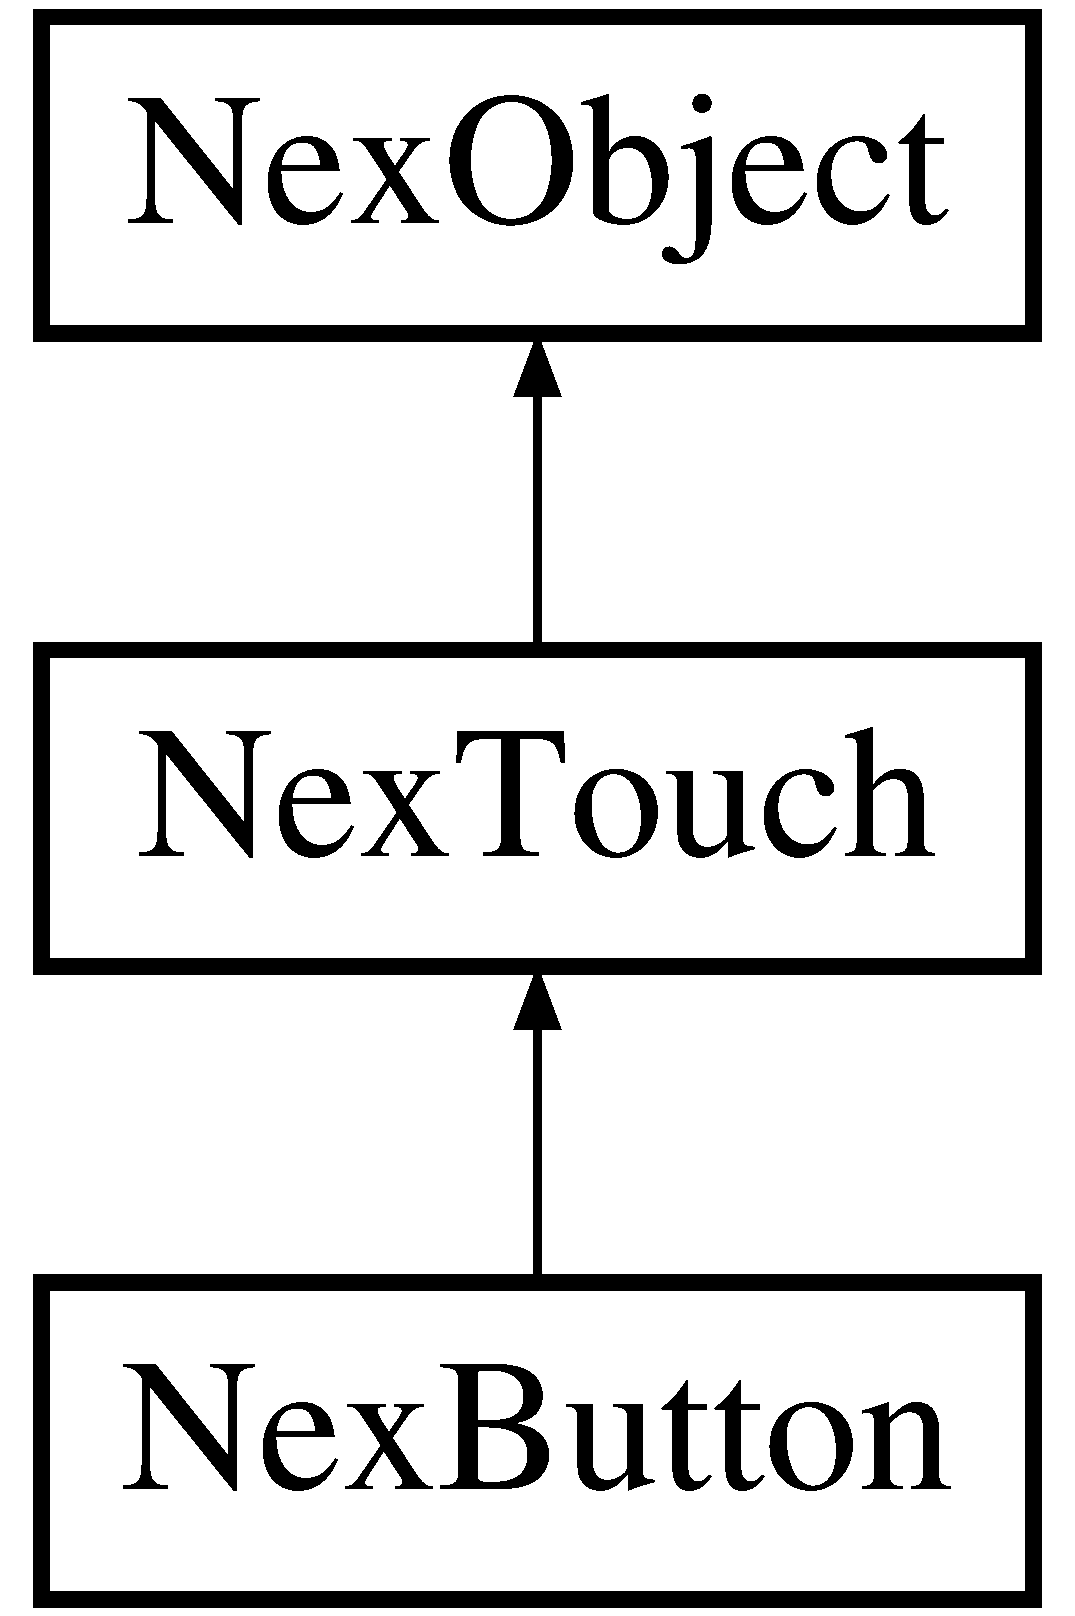
\includegraphics[height=3.000000cm]{class_nex_button}
\end{center}
\end{figure}
\subsection*{Public Member Functions}
\begin{DoxyCompactItemize}
\item 
\hyperlink{class_nex_button_a57d346614059bac40aff955a0dc9d76a}{Nex\+Button} (uint8\+\_\+t pid, uint8\+\_\+t cid, const char $\ast$name)
\item 
uint16\+\_\+t \hyperlink{class_nex_button_a5ba1f74aa94b41b98172e42583ee13d6}{get\+Text} (char $\ast$buffer, uint16\+\_\+t len)
\item 
bool \hyperlink{class_nex_button_a649dafc5afb1dc7f1fc1bde1e6270290}{set\+Text} (const char $\ast$buffer)
\item 
uint32\+\_\+t \hyperlink{class_nex_button_a85eb673a290ee35f3a73e9b02193fc70}{Get\+\_\+background\+\_\+color\+\_\+bco} (uint32\+\_\+t $\ast$number)
\item 
bool \hyperlink{class_nex_button_ae6ade99045d0f97594eac50adc7c12f7}{Set\+\_\+background\+\_\+color\+\_\+bco} (uint32\+\_\+t number)
\item 
uint32\+\_\+t \hyperlink{class_nex_button_abb5a765ca9079944757480a9fda1a6ac}{Get\+\_\+press\+\_\+background\+\_\+color\+\_\+bco2} (uint32\+\_\+t $\ast$number)
\item 
bool \hyperlink{class_nex_button_acdc1da7ffea8791a8237b201d572d1e3}{Set\+\_\+press\+\_\+background\+\_\+color\+\_\+bco2} (uint32\+\_\+t number)
\item 
uint32\+\_\+t \hyperlink{class_nex_button_a51b1b698696d7d4969ebb21754bb7e4d}{Get\+\_\+font\+\_\+color\+\_\+pco} (uint32\+\_\+t $\ast$number)
\item 
bool \hyperlink{class_nex_button_a9fbfe6df7a285e470fb8bc3fd77df00a}{Set\+\_\+font\+\_\+color\+\_\+pco} (uint32\+\_\+t number)
\item 
uint32\+\_\+t \hyperlink{class_nex_button_a970789126a0781810f499ae064fed942}{Get\+\_\+press\+\_\+font\+\_\+color\+\_\+pco2} (uint32\+\_\+t $\ast$number)
\item 
bool \hyperlink{class_nex_button_a5fe5e3331795ecb43eacf5aead7f5f4a}{Set\+\_\+press\+\_\+font\+\_\+color\+\_\+pco2} (uint32\+\_\+t number)
\item 
uint32\+\_\+t \hyperlink{class_nex_button_ab970c6e27b5d1d9082b0b3bf47ed9d47}{Get\+\_\+place\+\_\+xcen} (uint32\+\_\+t $\ast$number)
\item 
bool \hyperlink{class_nex_button_a76cdf6324e05d7a2c30f397e947e7cc7}{Set\+\_\+place\+\_\+xcen} (uint32\+\_\+t number)
\item 
uint32\+\_\+t \hyperlink{class_nex_button_aea0a8ea4e9a28ae3769414f2532483e9}{Get\+\_\+place\+\_\+ycen} (uint32\+\_\+t $\ast$number)
\item 
bool \hyperlink{class_nex_button_a50c8c3678dd815ec8d4e111c79251b53}{Set\+\_\+place\+\_\+ycen} (uint32\+\_\+t number)
\item 
uint32\+\_\+t \hyperlink{class_nex_button_aba350b47585e53ece6c5f6a83fe58698}{get\+Font} (uint32\+\_\+t $\ast$number)
\item 
bool \hyperlink{class_nex_button_a0fc4598f87578079127ea33a303962ff}{set\+Font} (uint32\+\_\+t number)
\item 
uint32\+\_\+t \hyperlink{class_nex_button_a4be9d316efb2e3c537fdbcbc74c5597c}{Get\+\_\+background\+\_\+cropi\+\_\+picc} (uint32\+\_\+t $\ast$number)
\item 
bool \hyperlink{class_nex_button_a71fc4f96d4700bd50cd6c937a0bfd43d}{Set\+\_\+background\+\_\+crop\+\_\+picc} (uint32\+\_\+t number)
\item 
uint32\+\_\+t \hyperlink{class_nex_button_ab85cad116c12d13fef9fcfb7dd7ae32e}{Get\+\_\+press\+\_\+background\+\_\+crop\+\_\+picc2} (uint32\+\_\+t $\ast$number)
\item 
bool \hyperlink{class_nex_button_a8f63f08fa00609546011b0a66e7070a7}{Set\+\_\+press\+\_\+background\+\_\+crop\+\_\+picc2} (uint32\+\_\+t number)
\item 
uint32\+\_\+t \hyperlink{class_nex_button_a81c5a95583a9561f4a188b3e3e082280}{Get\+\_\+background\+\_\+image\+\_\+pic} (uint32\+\_\+t $\ast$number)
\item 
bool \hyperlink{class_nex_button_a926c09d2615d74ef67d577c2934e2982}{Set\+\_\+background\+\_\+image\+\_\+pic} (uint32\+\_\+t number)
\item 
uint32\+\_\+t \hyperlink{class_nex_button_afce48613e87933b48e3b29901633c341}{Get\+\_\+press\+\_\+background\+\_\+image\+\_\+pic2} (uint32\+\_\+t $\ast$number)
\item 
bool \hyperlink{class_nex_button_a2c1ded80df08c3726347b8acc68d1678}{Set\+\_\+press\+\_\+background\+\_\+image\+\_\+pic2} (uint32\+\_\+t number)
\end{DoxyCompactItemize}
\subsection*{Additional Inherited Members}


\subsection{Detailed Description}
\hyperlink{class_nex_button}{Nex\+Button} component.

Commonly, you want to do something after push and pop it. It is recommanded that only call \hyperlink{class_nex_touch_a4da1c4fcdfadb7eabfb9ccaba9ecad11}{Nex\+Touch\+::attach\+Pop} to satisfy your purpose.

\begin{DoxyWarning}{Warning}
Please do not call \hyperlink{class_nex_touch_a685a753aae5eb9fb9866a7807a310132}{Nex\+Touch\+::attach\+Push} on this component, even though you can. 
\end{DoxyWarning}


\subsection{Constructor \& Destructor Documentation}
\hypertarget{class_nex_button_a57d346614059bac40aff955a0dc9d76a}{\index{Nex\+Button@{Nex\+Button}!Nex\+Button@{Nex\+Button}}
\index{Nex\+Button@{Nex\+Button}!Nex\+Button@{Nex\+Button}}
\subsubsection[{Nex\+Button}]{\setlength{\rightskip}{0pt plus 5cm}Nex\+Button\+::\+Nex\+Button (
\begin{DoxyParamCaption}
\item[{uint8\+\_\+t}]{pid, }
\item[{uint8\+\_\+t}]{cid, }
\item[{const char $\ast$}]{name}
\end{DoxyParamCaption}
)}}\label{class_nex_button_a57d346614059bac40aff955a0dc9d76a}




Constructor.


\begin{DoxyParams}{Parameters}
{\em pid} & -\/ page id. \\
\hline
{\em cid} & -\/ component id. \\
\hline
{\em name} & -\/ pointer to an unique name in range of all components. \\
\hline
\end{DoxyParams}


\subsection{Member Function Documentation}
\hypertarget{class_nex_button_a85eb673a290ee35f3a73e9b02193fc70}{\index{Nex\+Button@{Nex\+Button}!Get\+\_\+background\+\_\+color\+\_\+bco@{Get\+\_\+background\+\_\+color\+\_\+bco}}
\index{Get\+\_\+background\+\_\+color\+\_\+bco@{Get\+\_\+background\+\_\+color\+\_\+bco}!Nex\+Button@{Nex\+Button}}
\subsubsection[{Get\+\_\+background\+\_\+color\+\_\+bco}]{\setlength{\rightskip}{0pt plus 5cm}uint32\+\_\+t Nex\+Button\+::\+Get\+\_\+background\+\_\+color\+\_\+bco (
\begin{DoxyParamCaption}
\item[{uint32\+\_\+t $\ast$}]{number}
\end{DoxyParamCaption}
)}}\label{class_nex_button_a85eb673a290ee35f3a73e9b02193fc70}
Get bco attribute of component


\begin{DoxyParams}{Parameters}
{\em number} & -\/ buffer storing data return \\
\hline
\end{DoxyParams}
\begin{DoxyReturn}{Returns}
the length of the data 
\end{DoxyReturn}
\hypertarget{class_nex_button_a4be9d316efb2e3c537fdbcbc74c5597c}{\index{Nex\+Button@{Nex\+Button}!Get\+\_\+background\+\_\+cropi\+\_\+picc@{Get\+\_\+background\+\_\+cropi\+\_\+picc}}
\index{Get\+\_\+background\+\_\+cropi\+\_\+picc@{Get\+\_\+background\+\_\+cropi\+\_\+picc}!Nex\+Button@{Nex\+Button}}
\subsubsection[{Get\+\_\+background\+\_\+cropi\+\_\+picc}]{\setlength{\rightskip}{0pt plus 5cm}uint32\+\_\+t Nex\+Button\+::\+Get\+\_\+background\+\_\+cropi\+\_\+picc (
\begin{DoxyParamCaption}
\item[{uint32\+\_\+t $\ast$}]{number}
\end{DoxyParamCaption}
)}}\label{class_nex_button_a4be9d316efb2e3c537fdbcbc74c5597c}
Get picc attribute of component


\begin{DoxyParams}{Parameters}
{\em number} & -\/ buffer storing data return \\
\hline
\end{DoxyParams}
\begin{DoxyReturn}{Returns}
the length of the data 
\end{DoxyReturn}
\hypertarget{class_nex_button_a81c5a95583a9561f4a188b3e3e082280}{\index{Nex\+Button@{Nex\+Button}!Get\+\_\+background\+\_\+image\+\_\+pic@{Get\+\_\+background\+\_\+image\+\_\+pic}}
\index{Get\+\_\+background\+\_\+image\+\_\+pic@{Get\+\_\+background\+\_\+image\+\_\+pic}!Nex\+Button@{Nex\+Button}}
\subsubsection[{Get\+\_\+background\+\_\+image\+\_\+pic}]{\setlength{\rightskip}{0pt plus 5cm}uint32\+\_\+t Nex\+Button\+::\+Get\+\_\+background\+\_\+image\+\_\+pic (
\begin{DoxyParamCaption}
\item[{uint32\+\_\+t $\ast$}]{number}
\end{DoxyParamCaption}
)}}\label{class_nex_button_a81c5a95583a9561f4a188b3e3e082280}
Get pic attribute of component


\begin{DoxyParams}{Parameters}
{\em number} & -\/ buffer storing data return \\
\hline
\end{DoxyParams}
\begin{DoxyReturn}{Returns}
the length of the data 
\end{DoxyReturn}
\hypertarget{class_nex_button_a51b1b698696d7d4969ebb21754bb7e4d}{\index{Nex\+Button@{Nex\+Button}!Get\+\_\+font\+\_\+color\+\_\+pco@{Get\+\_\+font\+\_\+color\+\_\+pco}}
\index{Get\+\_\+font\+\_\+color\+\_\+pco@{Get\+\_\+font\+\_\+color\+\_\+pco}!Nex\+Button@{Nex\+Button}}
\subsubsection[{Get\+\_\+font\+\_\+color\+\_\+pco}]{\setlength{\rightskip}{0pt plus 5cm}uint32\+\_\+t Nex\+Button\+::\+Get\+\_\+font\+\_\+color\+\_\+pco (
\begin{DoxyParamCaption}
\item[{uint32\+\_\+t $\ast$}]{number}
\end{DoxyParamCaption}
)}}\label{class_nex_button_a51b1b698696d7d4969ebb21754bb7e4d}
Get pco attribute of component


\begin{DoxyParams}{Parameters}
{\em number} & -\/ buffer storing data return \\
\hline
\end{DoxyParams}
\begin{DoxyReturn}{Returns}
the length of the data 
\end{DoxyReturn}
\hypertarget{class_nex_button_ab970c6e27b5d1d9082b0b3bf47ed9d47}{\index{Nex\+Button@{Nex\+Button}!Get\+\_\+place\+\_\+xcen@{Get\+\_\+place\+\_\+xcen}}
\index{Get\+\_\+place\+\_\+xcen@{Get\+\_\+place\+\_\+xcen}!Nex\+Button@{Nex\+Button}}
\subsubsection[{Get\+\_\+place\+\_\+xcen}]{\setlength{\rightskip}{0pt plus 5cm}uint32\+\_\+t Nex\+Button\+::\+Get\+\_\+place\+\_\+xcen (
\begin{DoxyParamCaption}
\item[{uint32\+\_\+t $\ast$}]{number}
\end{DoxyParamCaption}
)}}\label{class_nex_button_ab970c6e27b5d1d9082b0b3bf47ed9d47}
Get xcen attribute of component


\begin{DoxyParams}{Parameters}
{\em number} & -\/ buffer storing data return \\
\hline
\end{DoxyParams}
\begin{DoxyReturn}{Returns}
the length of the data 
\end{DoxyReturn}
\hypertarget{class_nex_button_aea0a8ea4e9a28ae3769414f2532483e9}{\index{Nex\+Button@{Nex\+Button}!Get\+\_\+place\+\_\+ycen@{Get\+\_\+place\+\_\+ycen}}
\index{Get\+\_\+place\+\_\+ycen@{Get\+\_\+place\+\_\+ycen}!Nex\+Button@{Nex\+Button}}
\subsubsection[{Get\+\_\+place\+\_\+ycen}]{\setlength{\rightskip}{0pt plus 5cm}uint32\+\_\+t Nex\+Button\+::\+Get\+\_\+place\+\_\+ycen (
\begin{DoxyParamCaption}
\item[{uint32\+\_\+t $\ast$}]{number}
\end{DoxyParamCaption}
)}}\label{class_nex_button_aea0a8ea4e9a28ae3769414f2532483e9}
Get ycen attribute of component


\begin{DoxyParams}{Parameters}
{\em number} & -\/ buffer storing data return \\
\hline
\end{DoxyParams}
\begin{DoxyReturn}{Returns}
the length of the data 
\end{DoxyReturn}
\hypertarget{class_nex_button_abb5a765ca9079944757480a9fda1a6ac}{\index{Nex\+Button@{Nex\+Button}!Get\+\_\+press\+\_\+background\+\_\+color\+\_\+bco2@{Get\+\_\+press\+\_\+background\+\_\+color\+\_\+bco2}}
\index{Get\+\_\+press\+\_\+background\+\_\+color\+\_\+bco2@{Get\+\_\+press\+\_\+background\+\_\+color\+\_\+bco2}!Nex\+Button@{Nex\+Button}}
\subsubsection[{Get\+\_\+press\+\_\+background\+\_\+color\+\_\+bco2}]{\setlength{\rightskip}{0pt plus 5cm}uint32\+\_\+t Nex\+Button\+::\+Get\+\_\+press\+\_\+background\+\_\+color\+\_\+bco2 (
\begin{DoxyParamCaption}
\item[{uint32\+\_\+t $\ast$}]{number}
\end{DoxyParamCaption}
)}}\label{class_nex_button_abb5a765ca9079944757480a9fda1a6ac}
Get bco2 attribute of component


\begin{DoxyParams}{Parameters}
{\em number} & -\/ buffer storing data return \\
\hline
\end{DoxyParams}
\begin{DoxyReturn}{Returns}
the length of the data 
\end{DoxyReturn}
\hypertarget{class_nex_button_ab85cad116c12d13fef9fcfb7dd7ae32e}{\index{Nex\+Button@{Nex\+Button}!Get\+\_\+press\+\_\+background\+\_\+crop\+\_\+picc2@{Get\+\_\+press\+\_\+background\+\_\+crop\+\_\+picc2}}
\index{Get\+\_\+press\+\_\+background\+\_\+crop\+\_\+picc2@{Get\+\_\+press\+\_\+background\+\_\+crop\+\_\+picc2}!Nex\+Button@{Nex\+Button}}
\subsubsection[{Get\+\_\+press\+\_\+background\+\_\+crop\+\_\+picc2}]{\setlength{\rightskip}{0pt plus 5cm}uint32\+\_\+t Nex\+Button\+::\+Get\+\_\+press\+\_\+background\+\_\+crop\+\_\+picc2 (
\begin{DoxyParamCaption}
\item[{uint32\+\_\+t $\ast$}]{number}
\end{DoxyParamCaption}
)}}\label{class_nex_button_ab85cad116c12d13fef9fcfb7dd7ae32e}
Get picc2 attribute of component


\begin{DoxyParams}{Parameters}
{\em number} & -\/ buffer storing data return \\
\hline
\end{DoxyParams}
\begin{DoxyReturn}{Returns}
the length of the data 
\end{DoxyReturn}
\hypertarget{class_nex_button_afce48613e87933b48e3b29901633c341}{\index{Nex\+Button@{Nex\+Button}!Get\+\_\+press\+\_\+background\+\_\+image\+\_\+pic2@{Get\+\_\+press\+\_\+background\+\_\+image\+\_\+pic2}}
\index{Get\+\_\+press\+\_\+background\+\_\+image\+\_\+pic2@{Get\+\_\+press\+\_\+background\+\_\+image\+\_\+pic2}!Nex\+Button@{Nex\+Button}}
\subsubsection[{Get\+\_\+press\+\_\+background\+\_\+image\+\_\+pic2}]{\setlength{\rightskip}{0pt plus 5cm}uint32\+\_\+t Nex\+Button\+::\+Get\+\_\+press\+\_\+background\+\_\+image\+\_\+pic2 (
\begin{DoxyParamCaption}
\item[{uint32\+\_\+t $\ast$}]{number}
\end{DoxyParamCaption}
)}}\label{class_nex_button_afce48613e87933b48e3b29901633c341}
Get pic2 attribute of component


\begin{DoxyParams}{Parameters}
{\em number} & -\/ buffer storing data return \\
\hline
\end{DoxyParams}
\begin{DoxyReturn}{Returns}
the length of the data 
\end{DoxyReturn}
\hypertarget{class_nex_button_a970789126a0781810f499ae064fed942}{\index{Nex\+Button@{Nex\+Button}!Get\+\_\+press\+\_\+font\+\_\+color\+\_\+pco2@{Get\+\_\+press\+\_\+font\+\_\+color\+\_\+pco2}}
\index{Get\+\_\+press\+\_\+font\+\_\+color\+\_\+pco2@{Get\+\_\+press\+\_\+font\+\_\+color\+\_\+pco2}!Nex\+Button@{Nex\+Button}}
\subsubsection[{Get\+\_\+press\+\_\+font\+\_\+color\+\_\+pco2}]{\setlength{\rightskip}{0pt plus 5cm}uint32\+\_\+t Nex\+Button\+::\+Get\+\_\+press\+\_\+font\+\_\+color\+\_\+pco2 (
\begin{DoxyParamCaption}
\item[{uint32\+\_\+t $\ast$}]{number}
\end{DoxyParamCaption}
)}}\label{class_nex_button_a970789126a0781810f499ae064fed942}
Get pco2 attribute of component


\begin{DoxyParams}{Parameters}
{\em number} & -\/ buffer storing data return \\
\hline
\end{DoxyParams}
\begin{DoxyReturn}{Returns}
the length of the data 
\end{DoxyReturn}
\hypertarget{class_nex_button_aba350b47585e53ece6c5f6a83fe58698}{\index{Nex\+Button@{Nex\+Button}!get\+Font@{get\+Font}}
\index{get\+Font@{get\+Font}!Nex\+Button@{Nex\+Button}}
\subsubsection[{get\+Font}]{\setlength{\rightskip}{0pt plus 5cm}uint32\+\_\+t Nex\+Button\+::get\+Font (
\begin{DoxyParamCaption}
\item[{uint32\+\_\+t $\ast$}]{number}
\end{DoxyParamCaption}
)}}\label{class_nex_button_aba350b47585e53ece6c5f6a83fe58698}
Get font attribute of component


\begin{DoxyParams}{Parameters}
{\em number} & -\/ buffer storing data return \\
\hline
\end{DoxyParams}
\begin{DoxyReturn}{Returns}
the length of the data 
\end{DoxyReturn}
\hypertarget{class_nex_button_a5ba1f74aa94b41b98172e42583ee13d6}{\index{Nex\+Button@{Nex\+Button}!get\+Text@{get\+Text}}
\index{get\+Text@{get\+Text}!Nex\+Button@{Nex\+Button}}
\subsubsection[{get\+Text}]{\setlength{\rightskip}{0pt plus 5cm}uint16\+\_\+t Nex\+Button\+::get\+Text (
\begin{DoxyParamCaption}
\item[{char $\ast$}]{buffer, }
\item[{uint16\+\_\+t}]{len}
\end{DoxyParamCaption}
)}}\label{class_nex_button_a5ba1f74aa94b41b98172e42583ee13d6}
Get text attribute of component.


\begin{DoxyParams}{Parameters}
{\em buffer} & -\/ buffer storing text returned. \\
\hline
{\em len} & -\/ length of buffer. \\
\hline
\end{DoxyParams}
\begin{DoxyReturn}{Returns}
The real length of text returned. 
\end{DoxyReturn}
\hypertarget{class_nex_button_ae6ade99045d0f97594eac50adc7c12f7}{\index{Nex\+Button@{Nex\+Button}!Set\+\_\+background\+\_\+color\+\_\+bco@{Set\+\_\+background\+\_\+color\+\_\+bco}}
\index{Set\+\_\+background\+\_\+color\+\_\+bco@{Set\+\_\+background\+\_\+color\+\_\+bco}!Nex\+Button@{Nex\+Button}}
\subsubsection[{Set\+\_\+background\+\_\+color\+\_\+bco}]{\setlength{\rightskip}{0pt plus 5cm}bool Nex\+Button\+::\+Set\+\_\+background\+\_\+color\+\_\+bco (
\begin{DoxyParamCaption}
\item[{uint32\+\_\+t}]{number}
\end{DoxyParamCaption}
)}}\label{class_nex_button_ae6ade99045d0f97594eac50adc7c12f7}
Set bco attribute of component


\begin{DoxyParams}{Parameters}
{\em number} & -\/ To set up the data \\
\hline
\end{DoxyParams}
\begin{DoxyReturn}{Returns}
true if success, false for failure 
\end{DoxyReturn}
\hypertarget{class_nex_button_a71fc4f96d4700bd50cd6c937a0bfd43d}{\index{Nex\+Button@{Nex\+Button}!Set\+\_\+background\+\_\+crop\+\_\+picc@{Set\+\_\+background\+\_\+crop\+\_\+picc}}
\index{Set\+\_\+background\+\_\+crop\+\_\+picc@{Set\+\_\+background\+\_\+crop\+\_\+picc}!Nex\+Button@{Nex\+Button}}
\subsubsection[{Set\+\_\+background\+\_\+crop\+\_\+picc}]{\setlength{\rightskip}{0pt plus 5cm}bool Nex\+Button\+::\+Set\+\_\+background\+\_\+crop\+\_\+picc (
\begin{DoxyParamCaption}
\item[{uint32\+\_\+t}]{number}
\end{DoxyParamCaption}
)}}\label{class_nex_button_a71fc4f96d4700bd50cd6c937a0bfd43d}
Set picc attribute of component


\begin{DoxyParams}{Parameters}
{\em number} & -\/ To set up the data \\
\hline
\end{DoxyParams}
\begin{DoxyReturn}{Returns}
true if success, false for failure 
\end{DoxyReturn}
\hypertarget{class_nex_button_a926c09d2615d74ef67d577c2934e2982}{\index{Nex\+Button@{Nex\+Button}!Set\+\_\+background\+\_\+image\+\_\+pic@{Set\+\_\+background\+\_\+image\+\_\+pic}}
\index{Set\+\_\+background\+\_\+image\+\_\+pic@{Set\+\_\+background\+\_\+image\+\_\+pic}!Nex\+Button@{Nex\+Button}}
\subsubsection[{Set\+\_\+background\+\_\+image\+\_\+pic}]{\setlength{\rightskip}{0pt plus 5cm}bool Nex\+Button\+::\+Set\+\_\+background\+\_\+image\+\_\+pic (
\begin{DoxyParamCaption}
\item[{uint32\+\_\+t}]{number}
\end{DoxyParamCaption}
)}}\label{class_nex_button_a926c09d2615d74ef67d577c2934e2982}
Set pic attribute of component


\begin{DoxyParams}{Parameters}
{\em number} & -\/ To set up the data \\
\hline
\end{DoxyParams}
\begin{DoxyReturn}{Returns}
true if success, false for failure 
\end{DoxyReturn}
\hypertarget{class_nex_button_a9fbfe6df7a285e470fb8bc3fd77df00a}{\index{Nex\+Button@{Nex\+Button}!Set\+\_\+font\+\_\+color\+\_\+pco@{Set\+\_\+font\+\_\+color\+\_\+pco}}
\index{Set\+\_\+font\+\_\+color\+\_\+pco@{Set\+\_\+font\+\_\+color\+\_\+pco}!Nex\+Button@{Nex\+Button}}
\subsubsection[{Set\+\_\+font\+\_\+color\+\_\+pco}]{\setlength{\rightskip}{0pt plus 5cm}bool Nex\+Button\+::\+Set\+\_\+font\+\_\+color\+\_\+pco (
\begin{DoxyParamCaption}
\item[{uint32\+\_\+t}]{number}
\end{DoxyParamCaption}
)}}\label{class_nex_button_a9fbfe6df7a285e470fb8bc3fd77df00a}
Set pco attribute of component


\begin{DoxyParams}{Parameters}
{\em number} & -\/ To set up the data \\
\hline
\end{DoxyParams}
\begin{DoxyReturn}{Returns}
true if success, false for failure 
\end{DoxyReturn}
\hypertarget{class_nex_button_a76cdf6324e05d7a2c30f397e947e7cc7}{\index{Nex\+Button@{Nex\+Button}!Set\+\_\+place\+\_\+xcen@{Set\+\_\+place\+\_\+xcen}}
\index{Set\+\_\+place\+\_\+xcen@{Set\+\_\+place\+\_\+xcen}!Nex\+Button@{Nex\+Button}}
\subsubsection[{Set\+\_\+place\+\_\+xcen}]{\setlength{\rightskip}{0pt plus 5cm}bool Nex\+Button\+::\+Set\+\_\+place\+\_\+xcen (
\begin{DoxyParamCaption}
\item[{uint32\+\_\+t}]{number}
\end{DoxyParamCaption}
)}}\label{class_nex_button_a76cdf6324e05d7a2c30f397e947e7cc7}
Set xcen attribute of component


\begin{DoxyParams}{Parameters}
{\em number} & -\/ To set up the data \\
\hline
\end{DoxyParams}
\begin{DoxyReturn}{Returns}
true if success, false for failure 
\end{DoxyReturn}
\hypertarget{class_nex_button_a50c8c3678dd815ec8d4e111c79251b53}{\index{Nex\+Button@{Nex\+Button}!Set\+\_\+place\+\_\+ycen@{Set\+\_\+place\+\_\+ycen}}
\index{Set\+\_\+place\+\_\+ycen@{Set\+\_\+place\+\_\+ycen}!Nex\+Button@{Nex\+Button}}
\subsubsection[{Set\+\_\+place\+\_\+ycen}]{\setlength{\rightskip}{0pt plus 5cm}bool Nex\+Button\+::\+Set\+\_\+place\+\_\+ycen (
\begin{DoxyParamCaption}
\item[{uint32\+\_\+t}]{number}
\end{DoxyParamCaption}
)}}\label{class_nex_button_a50c8c3678dd815ec8d4e111c79251b53}
Set ycen attribute of component


\begin{DoxyParams}{Parameters}
{\em number} & -\/ To set up the data \\
\hline
\end{DoxyParams}
\begin{DoxyReturn}{Returns}
true if success, false for failure 
\end{DoxyReturn}
\hypertarget{class_nex_button_acdc1da7ffea8791a8237b201d572d1e3}{\index{Nex\+Button@{Nex\+Button}!Set\+\_\+press\+\_\+background\+\_\+color\+\_\+bco2@{Set\+\_\+press\+\_\+background\+\_\+color\+\_\+bco2}}
\index{Set\+\_\+press\+\_\+background\+\_\+color\+\_\+bco2@{Set\+\_\+press\+\_\+background\+\_\+color\+\_\+bco2}!Nex\+Button@{Nex\+Button}}
\subsubsection[{Set\+\_\+press\+\_\+background\+\_\+color\+\_\+bco2}]{\setlength{\rightskip}{0pt plus 5cm}bool Nex\+Button\+::\+Set\+\_\+press\+\_\+background\+\_\+color\+\_\+bco2 (
\begin{DoxyParamCaption}
\item[{uint32\+\_\+t}]{number}
\end{DoxyParamCaption}
)}}\label{class_nex_button_acdc1da7ffea8791a8237b201d572d1e3}
Set bco2 attribute of component


\begin{DoxyParams}{Parameters}
{\em number} & -\/ To set up the data \\
\hline
\end{DoxyParams}
\begin{DoxyReturn}{Returns}
true if success, false for failure 
\end{DoxyReturn}
\hypertarget{class_nex_button_a8f63f08fa00609546011b0a66e7070a7}{\index{Nex\+Button@{Nex\+Button}!Set\+\_\+press\+\_\+background\+\_\+crop\+\_\+picc2@{Set\+\_\+press\+\_\+background\+\_\+crop\+\_\+picc2}}
\index{Set\+\_\+press\+\_\+background\+\_\+crop\+\_\+picc2@{Set\+\_\+press\+\_\+background\+\_\+crop\+\_\+picc2}!Nex\+Button@{Nex\+Button}}
\subsubsection[{Set\+\_\+press\+\_\+background\+\_\+crop\+\_\+picc2}]{\setlength{\rightskip}{0pt plus 5cm}bool Nex\+Button\+::\+Set\+\_\+press\+\_\+background\+\_\+crop\+\_\+picc2 (
\begin{DoxyParamCaption}
\item[{uint32\+\_\+t}]{number}
\end{DoxyParamCaption}
)}}\label{class_nex_button_a8f63f08fa00609546011b0a66e7070a7}
Set picc2 attribute of component


\begin{DoxyParams}{Parameters}
{\em number} & -\/ To set up the data \\
\hline
\end{DoxyParams}
\begin{DoxyReturn}{Returns}
true if success, false for failure 
\end{DoxyReturn}
\hypertarget{class_nex_button_a2c1ded80df08c3726347b8acc68d1678}{\index{Nex\+Button@{Nex\+Button}!Set\+\_\+press\+\_\+background\+\_\+image\+\_\+pic2@{Set\+\_\+press\+\_\+background\+\_\+image\+\_\+pic2}}
\index{Set\+\_\+press\+\_\+background\+\_\+image\+\_\+pic2@{Set\+\_\+press\+\_\+background\+\_\+image\+\_\+pic2}!Nex\+Button@{Nex\+Button}}
\subsubsection[{Set\+\_\+press\+\_\+background\+\_\+image\+\_\+pic2}]{\setlength{\rightskip}{0pt plus 5cm}bool Nex\+Button\+::\+Set\+\_\+press\+\_\+background\+\_\+image\+\_\+pic2 (
\begin{DoxyParamCaption}
\item[{uint32\+\_\+t}]{number}
\end{DoxyParamCaption}
)}}\label{class_nex_button_a2c1ded80df08c3726347b8acc68d1678}
Set pic2 attribute of component


\begin{DoxyParams}{Parameters}
{\em number} & -\/ To set up the data \\
\hline
\end{DoxyParams}
\begin{DoxyReturn}{Returns}
true if success, false for failure 
\end{DoxyReturn}
\hypertarget{class_nex_button_a5fe5e3331795ecb43eacf5aead7f5f4a}{\index{Nex\+Button@{Nex\+Button}!Set\+\_\+press\+\_\+font\+\_\+color\+\_\+pco2@{Set\+\_\+press\+\_\+font\+\_\+color\+\_\+pco2}}
\index{Set\+\_\+press\+\_\+font\+\_\+color\+\_\+pco2@{Set\+\_\+press\+\_\+font\+\_\+color\+\_\+pco2}!Nex\+Button@{Nex\+Button}}
\subsubsection[{Set\+\_\+press\+\_\+font\+\_\+color\+\_\+pco2}]{\setlength{\rightskip}{0pt plus 5cm}bool Nex\+Button\+::\+Set\+\_\+press\+\_\+font\+\_\+color\+\_\+pco2 (
\begin{DoxyParamCaption}
\item[{uint32\+\_\+t}]{number}
\end{DoxyParamCaption}
)}}\label{class_nex_button_a5fe5e3331795ecb43eacf5aead7f5f4a}
Set pco2 attribute of component


\begin{DoxyParams}{Parameters}
{\em number} & -\/ To set up the data \\
\hline
\end{DoxyParams}
\begin{DoxyReturn}{Returns}
true if success, false for failure 
\end{DoxyReturn}
\hypertarget{class_nex_button_a0fc4598f87578079127ea33a303962ff}{\index{Nex\+Button@{Nex\+Button}!set\+Font@{set\+Font}}
\index{set\+Font@{set\+Font}!Nex\+Button@{Nex\+Button}}
\subsubsection[{set\+Font}]{\setlength{\rightskip}{0pt plus 5cm}bool Nex\+Button\+::set\+Font (
\begin{DoxyParamCaption}
\item[{uint32\+\_\+t}]{number}
\end{DoxyParamCaption}
)}}\label{class_nex_button_a0fc4598f87578079127ea33a303962ff}
Set font attribute of component


\begin{DoxyParams}{Parameters}
{\em number} & -\/ To set up the data \\
\hline
\end{DoxyParams}
\begin{DoxyReturn}{Returns}
true if success, false for failure 
\end{DoxyReturn}
\hypertarget{class_nex_button_a649dafc5afb1dc7f1fc1bde1e6270290}{\index{Nex\+Button@{Nex\+Button}!set\+Text@{set\+Text}}
\index{set\+Text@{set\+Text}!Nex\+Button@{Nex\+Button}}
\subsubsection[{set\+Text}]{\setlength{\rightskip}{0pt plus 5cm}bool Nex\+Button\+::set\+Text (
\begin{DoxyParamCaption}
\item[{const char $\ast$}]{buffer}
\end{DoxyParamCaption}
)}}\label{class_nex_button_a649dafc5afb1dc7f1fc1bde1e6270290}
Set text attribute of component.


\begin{DoxyParams}{Parameters}
{\em buffer} & -\/ text buffer terminated with '\textbackslash{}0'. \\
\hline
\end{DoxyParams}
\begin{DoxyReturn}{Returns}
true if success, false for failure. 
\end{DoxyReturn}


The documentation for this class was generated from the following files\+:\begin{DoxyCompactItemize}
\item 
\hyperlink{_nex_button_8h}{Nex\+Button.\+h}\item 
\hyperlink{_nex_button_8cpp}{Nex\+Button.\+cpp}\end{DoxyCompactItemize}

\hypertarget{class_nex_checkbox}{\section{Nex\+Checkbox Class Reference}
\label{class_nex_checkbox}\index{Nex\+Checkbox@{Nex\+Checkbox}}
}


{\ttfamily \#include $<$Nex\+Checkbox.\+h$>$}

Inheritance diagram for Nex\+Checkbox\+:\begin{figure}[H]
\begin{center}
\leavevmode
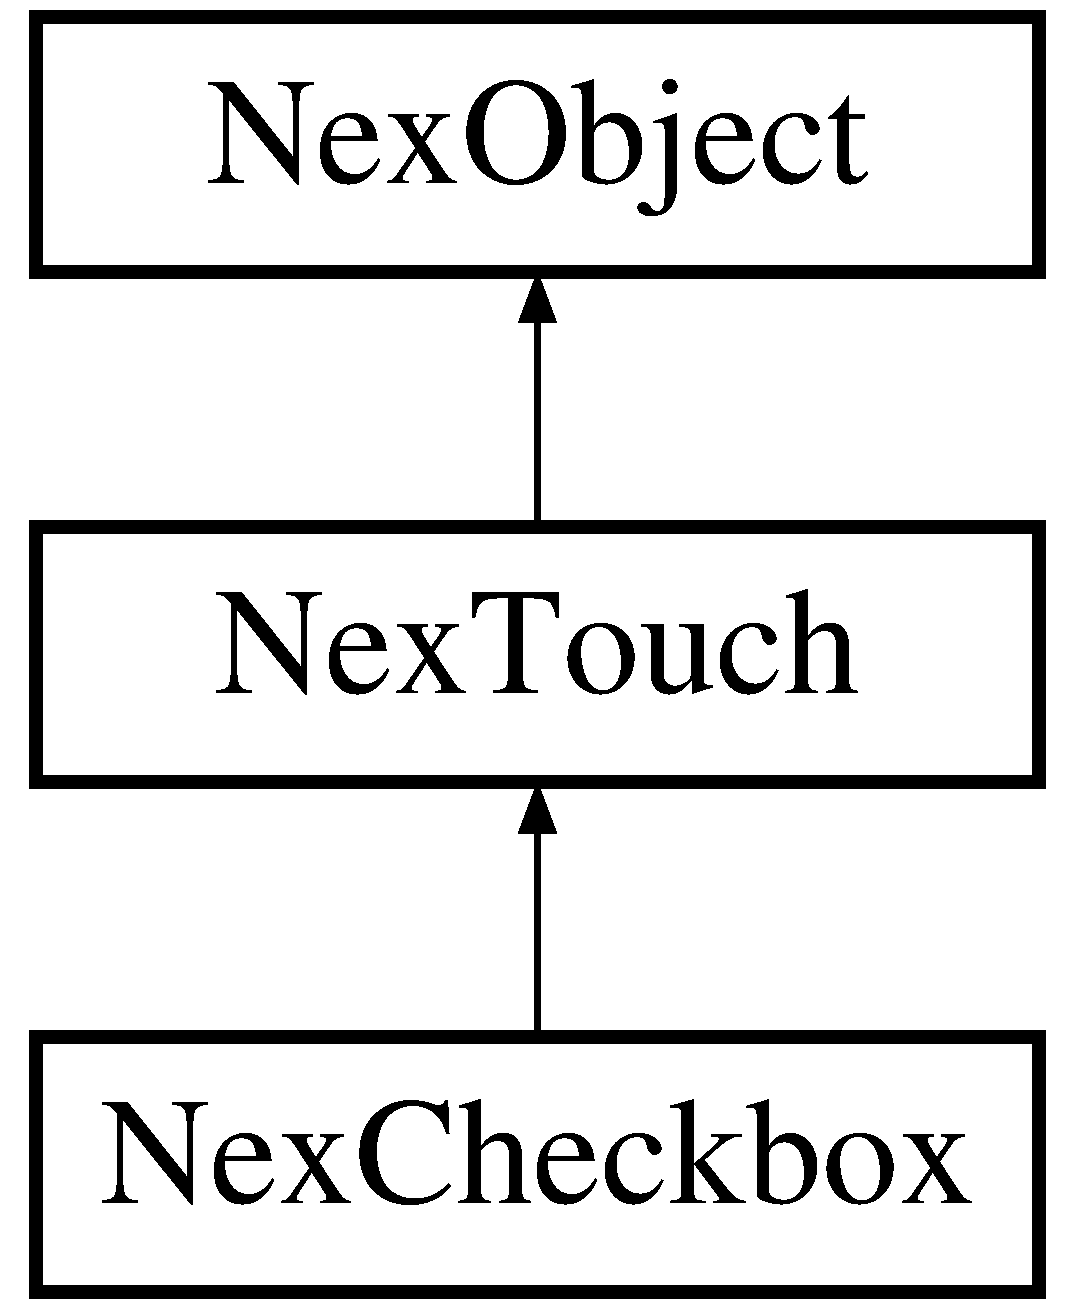
\includegraphics[height=3.000000cm]{class_nex_checkbox}
\end{center}
\end{figure}
\subsection*{Public Member Functions}
\begin{DoxyCompactItemize}
\item 
\hyperlink{class_nex_checkbox_a8aa4ea60796bdce0de0de3dd675ef56a}{Nex\+Checkbox} (uint8\+\_\+t pid, uint8\+\_\+t cid, const char $\ast$name)
\item 
uint32\+\_\+t \hyperlink{class_nex_checkbox_a6832110a49f9bbbb14a54f36db020d44}{get\+Value} (uint32\+\_\+t $\ast$number)
\item 
bool \hyperlink{class_nex_checkbox_aa932e7c45765400618dce1804766264b}{set\+Value} (uint32\+\_\+t number)
\item 
uint32\+\_\+t \hyperlink{class_nex_checkbox_abca30f46ecb7a4c88d816af85fa7f777}{Get\+\_\+background\+\_\+color\+\_\+bco} (uint32\+\_\+t $\ast$number)
\item 
bool \hyperlink{class_nex_checkbox_ab430ba5908c84fea8ab910002581350a}{Set\+\_\+background\+\_\+color\+\_\+bco} (uint32\+\_\+t number)
\item 
uint32\+\_\+t \hyperlink{class_nex_checkbox_a93fbcf8796f156e6700ebf3e13abfce6}{Get\+\_\+font\+\_\+color\+\_\+pco} (uint32\+\_\+t $\ast$number)
\item 
bool \hyperlink{class_nex_checkbox_aa1d52cc0170f11ec85263770fe77db2a}{Set\+\_\+font\+\_\+color\+\_\+pco} (uint32\+\_\+t number)
\end{DoxyCompactItemize}
\subsection*{Additional Inherited Members}


\subsection{Detailed Description}
\hyperlink{class_nex_button}{Nex\+Button} component.

Commonly, you want to do something after push and pop it. It is recommanded that only call \hyperlink{class_nex_touch_a4da1c4fcdfadb7eabfb9ccaba9ecad11}{Nex\+Touch\+::attach\+Pop} to satisfy your purpose.

\begin{DoxyWarning}{Warning}
Please do not call \hyperlink{class_nex_touch_a685a753aae5eb9fb9866a7807a310132}{Nex\+Touch\+::attach\+Push} on this component, even though you can. 
\end{DoxyWarning}


\subsection{Constructor \& Destructor Documentation}
\hypertarget{class_nex_checkbox_a8aa4ea60796bdce0de0de3dd675ef56a}{\index{Nex\+Checkbox@{Nex\+Checkbox}!Nex\+Checkbox@{Nex\+Checkbox}}
\index{Nex\+Checkbox@{Nex\+Checkbox}!Nex\+Checkbox@{Nex\+Checkbox}}
\subsubsection[{Nex\+Checkbox}]{\setlength{\rightskip}{0pt plus 5cm}Nex\+Checkbox\+::\+Nex\+Checkbox (
\begin{DoxyParamCaption}
\item[{uint8\+\_\+t}]{pid, }
\item[{uint8\+\_\+t}]{cid, }
\item[{const char $\ast$}]{name}
\end{DoxyParamCaption}
)}}\label{class_nex_checkbox_a8aa4ea60796bdce0de0de3dd675ef56a}




Constructor.


\begin{DoxyParams}{Parameters}
{\em pid} & -\/ page id. \\
\hline
{\em cid} & -\/ component id. \\
\hline
{\em name} & -\/ pointer to an unique name in range of all components. \\
\hline
\end{DoxyParams}


\subsection{Member Function Documentation}
\hypertarget{class_nex_checkbox_abca30f46ecb7a4c88d816af85fa7f777}{\index{Nex\+Checkbox@{Nex\+Checkbox}!Get\+\_\+background\+\_\+color\+\_\+bco@{Get\+\_\+background\+\_\+color\+\_\+bco}}
\index{Get\+\_\+background\+\_\+color\+\_\+bco@{Get\+\_\+background\+\_\+color\+\_\+bco}!Nex\+Checkbox@{Nex\+Checkbox}}
\subsubsection[{Get\+\_\+background\+\_\+color\+\_\+bco}]{\setlength{\rightskip}{0pt plus 5cm}uint32\+\_\+t Nex\+Checkbox\+::\+Get\+\_\+background\+\_\+color\+\_\+bco (
\begin{DoxyParamCaption}
\item[{uint32\+\_\+t $\ast$}]{number}
\end{DoxyParamCaption}
)}}\label{class_nex_checkbox_abca30f46ecb7a4c88d816af85fa7f777}
Get bco attribute of component


\begin{DoxyParams}{Parameters}
{\em number} & -\/ buffer storing data retur \\
\hline
\end{DoxyParams}
\begin{DoxyReturn}{Returns}
the length of the data 
\end{DoxyReturn}
\hypertarget{class_nex_checkbox_a93fbcf8796f156e6700ebf3e13abfce6}{\index{Nex\+Checkbox@{Nex\+Checkbox}!Get\+\_\+font\+\_\+color\+\_\+pco@{Get\+\_\+font\+\_\+color\+\_\+pco}}
\index{Get\+\_\+font\+\_\+color\+\_\+pco@{Get\+\_\+font\+\_\+color\+\_\+pco}!Nex\+Checkbox@{Nex\+Checkbox}}
\subsubsection[{Get\+\_\+font\+\_\+color\+\_\+pco}]{\setlength{\rightskip}{0pt plus 5cm}uint32\+\_\+t Nex\+Checkbox\+::\+Get\+\_\+font\+\_\+color\+\_\+pco (
\begin{DoxyParamCaption}
\item[{uint32\+\_\+t $\ast$}]{number}
\end{DoxyParamCaption}
)}}\label{class_nex_checkbox_a93fbcf8796f156e6700ebf3e13abfce6}
Get pco attribute of component


\begin{DoxyParams}{Parameters}
{\em number} & -\/ buffer storing data retur \\
\hline
\end{DoxyParams}
\begin{DoxyReturn}{Returns}
the length of the data 
\end{DoxyReturn}
\hypertarget{class_nex_checkbox_a6832110a49f9bbbb14a54f36db020d44}{\index{Nex\+Checkbox@{Nex\+Checkbox}!get\+Value@{get\+Value}}
\index{get\+Value@{get\+Value}!Nex\+Checkbox@{Nex\+Checkbox}}
\subsubsection[{get\+Value}]{\setlength{\rightskip}{0pt plus 5cm}uint32\+\_\+t Nex\+Checkbox\+::get\+Value (
\begin{DoxyParamCaption}
\item[{uint32\+\_\+t $\ast$}]{number}
\end{DoxyParamCaption}
)}}\label{class_nex_checkbox_a6832110a49f9bbbb14a54f36db020d44}
Get val attribute of component


\begin{DoxyParams}{Parameters}
{\em number} & -\/ buffer storing data retur \\
\hline
\end{DoxyParams}
\begin{DoxyReturn}{Returns}
the length of the data 
\end{DoxyReturn}
\hypertarget{class_nex_checkbox_ab430ba5908c84fea8ab910002581350a}{\index{Nex\+Checkbox@{Nex\+Checkbox}!Set\+\_\+background\+\_\+color\+\_\+bco@{Set\+\_\+background\+\_\+color\+\_\+bco}}
\index{Set\+\_\+background\+\_\+color\+\_\+bco@{Set\+\_\+background\+\_\+color\+\_\+bco}!Nex\+Checkbox@{Nex\+Checkbox}}
\subsubsection[{Set\+\_\+background\+\_\+color\+\_\+bco}]{\setlength{\rightskip}{0pt plus 5cm}bool Nex\+Checkbox\+::\+Set\+\_\+background\+\_\+color\+\_\+bco (
\begin{DoxyParamCaption}
\item[{uint32\+\_\+t}]{number}
\end{DoxyParamCaption}
)}}\label{class_nex_checkbox_ab430ba5908c84fea8ab910002581350a}
Set bco attribute of component


\begin{DoxyParams}{Parameters}
{\em number} & -\/ To set up the data \\
\hline
\end{DoxyParams}
\begin{DoxyReturn}{Returns}
true if success, false for failure 
\end{DoxyReturn}
\hypertarget{class_nex_checkbox_aa1d52cc0170f11ec85263770fe77db2a}{\index{Nex\+Checkbox@{Nex\+Checkbox}!Set\+\_\+font\+\_\+color\+\_\+pco@{Set\+\_\+font\+\_\+color\+\_\+pco}}
\index{Set\+\_\+font\+\_\+color\+\_\+pco@{Set\+\_\+font\+\_\+color\+\_\+pco}!Nex\+Checkbox@{Nex\+Checkbox}}
\subsubsection[{Set\+\_\+font\+\_\+color\+\_\+pco}]{\setlength{\rightskip}{0pt plus 5cm}bool Nex\+Checkbox\+::\+Set\+\_\+font\+\_\+color\+\_\+pco (
\begin{DoxyParamCaption}
\item[{uint32\+\_\+t}]{number}
\end{DoxyParamCaption}
)}}\label{class_nex_checkbox_aa1d52cc0170f11ec85263770fe77db2a}
Set pco attribute of component


\begin{DoxyParams}{Parameters}
{\em number} & -\/ To set up the data \\
\hline
\end{DoxyParams}
\begin{DoxyReturn}{Returns}
true if success, false for failure 
\end{DoxyReturn}
\hypertarget{class_nex_checkbox_aa932e7c45765400618dce1804766264b}{\index{Nex\+Checkbox@{Nex\+Checkbox}!set\+Value@{set\+Value}}
\index{set\+Value@{set\+Value}!Nex\+Checkbox@{Nex\+Checkbox}}
\subsubsection[{set\+Value}]{\setlength{\rightskip}{0pt plus 5cm}bool Nex\+Checkbox\+::set\+Value (
\begin{DoxyParamCaption}
\item[{uint32\+\_\+t}]{number}
\end{DoxyParamCaption}
)}}\label{class_nex_checkbox_aa932e7c45765400618dce1804766264b}
Set val attribute of component


\begin{DoxyParams}{Parameters}
{\em number} & -\/ To set up the data \\
\hline
\end{DoxyParams}
\begin{DoxyReturn}{Returns}
true if success, false for failure 
\end{DoxyReturn}


The documentation for this class was generated from the following files\+:\begin{DoxyCompactItemize}
\item 
\hyperlink{_nex_checkbox_8h}{Nex\+Checkbox.\+h}\item 
\hyperlink{_nex_checkbox_8cpp}{Nex\+Checkbox.\+cpp}\end{DoxyCompactItemize}

\hypertarget{class_nex_crop}{\section{Nex\+Crop Class Reference}
\label{class_nex_crop}\index{Nex\+Crop@{Nex\+Crop}}
}


{\ttfamily \#include $<$Nex\+Crop.\+h$>$}

Inheritance diagram for Nex\+Crop\+:\begin{figure}[H]
\begin{center}
\leavevmode
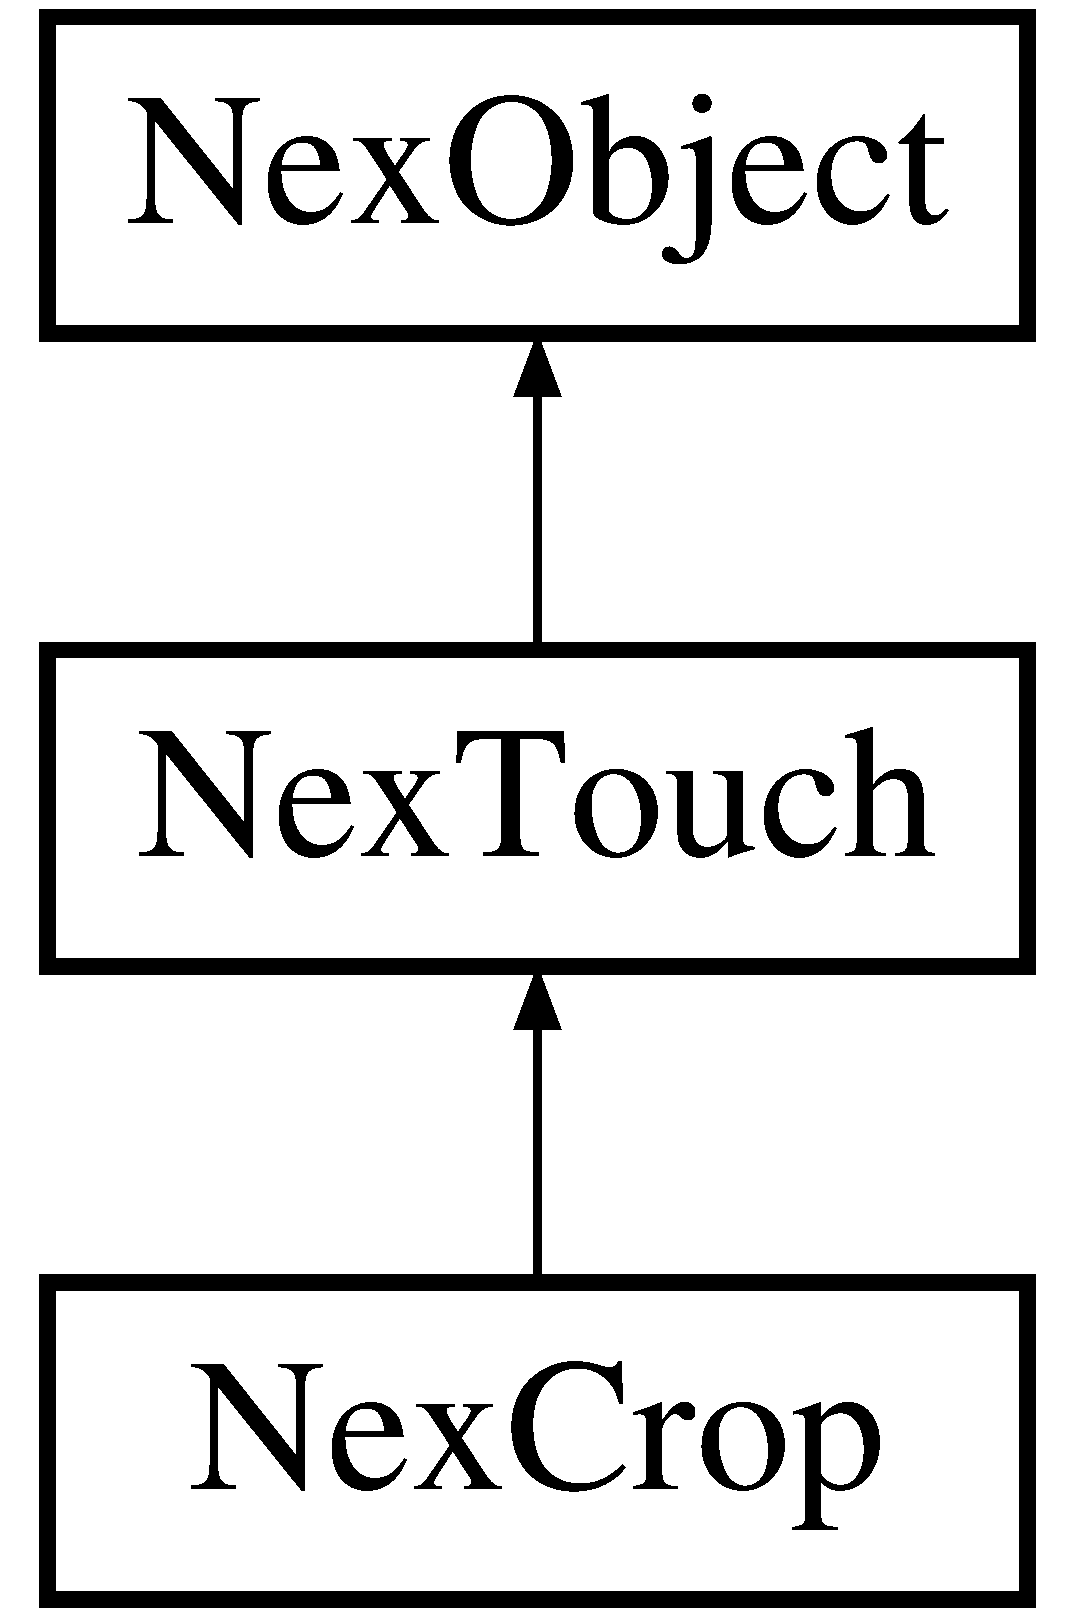
\includegraphics[height=3.000000cm]{class_nex_crop}
\end{center}
\end{figure}
\subsection*{Public Member Functions}
\begin{DoxyCompactItemize}
\item 
\hyperlink{class_nex_crop_a1a3a195d3da05cb832f91a2ef43f27d3}{Nex\+Crop} (uint8\+\_\+t pid, uint8\+\_\+t cid, const char $\ast$name)
\item 
bool \hyperlink{class_nex_crop_a19f824bea045bab4cc1afc5950259247}{Get\+\_\+background\+\_\+crop\+\_\+picc} (uint32\+\_\+t $\ast$number)
\item 
bool \hyperlink{class_nex_crop_aa85a69de5055c29f0a85406d10806bfe}{Set\+\_\+background\+\_\+crop\+\_\+picc} (uint32\+\_\+t number)
\item 
bool \hyperlink{class_nex_crop_a2cbfe125182626965dd530f14ab55885}{get\+Pic} (uint32\+\_\+t $\ast$number)
\item 
bool \hyperlink{class_nex_crop_aac34fc2f8ead1e330918089ea8a339db}{set\+Pic} (uint32\+\_\+t number)
\end{DoxyCompactItemize}
\subsection*{Additional Inherited Members}


\subsection{Detailed Description}
\hyperlink{class_nex_crop}{Nex\+Crop} component. 

\subsection{Constructor \& Destructor Documentation}
\hypertarget{class_nex_crop_a1a3a195d3da05cb832f91a2ef43f27d3}{\index{Nex\+Crop@{Nex\+Crop}!Nex\+Crop@{Nex\+Crop}}
\index{Nex\+Crop@{Nex\+Crop}!Nex\+Crop@{Nex\+Crop}}
\subsubsection[{Nex\+Crop}]{\setlength{\rightskip}{0pt plus 5cm}Nex\+Crop\+::\+Nex\+Crop (
\begin{DoxyParamCaption}
\item[{uint8\+\_\+t}]{pid, }
\item[{uint8\+\_\+t}]{cid, }
\item[{const char $\ast$}]{name}
\end{DoxyParamCaption}
)}}\label{class_nex_crop_a1a3a195d3da05cb832f91a2ef43f27d3}




Constructor.


\begin{DoxyParams}{Parameters}
{\em pid} & -\/ page id. \\
\hline
{\em cid} & -\/ component id. \\
\hline
{\em name} & -\/ pointer to an unique name in range of all components. \\
\hline
\end{DoxyParams}


\subsection{Member Function Documentation}
\hypertarget{class_nex_crop_a19f824bea045bab4cc1afc5950259247}{\index{Nex\+Crop@{Nex\+Crop}!Get\+\_\+background\+\_\+crop\+\_\+picc@{Get\+\_\+background\+\_\+crop\+\_\+picc}}
\index{Get\+\_\+background\+\_\+crop\+\_\+picc@{Get\+\_\+background\+\_\+crop\+\_\+picc}!Nex\+Crop@{Nex\+Crop}}
\subsubsection[{Get\+\_\+background\+\_\+crop\+\_\+picc}]{\setlength{\rightskip}{0pt plus 5cm}bool Nex\+Crop\+::\+Get\+\_\+background\+\_\+crop\+\_\+picc (
\begin{DoxyParamCaption}
\item[{uint32\+\_\+t $\ast$}]{number}
\end{DoxyParamCaption}
)}}\label{class_nex_crop_a19f824bea045bab4cc1afc5950259247}
Get the number of picture.


\begin{DoxyParams}{Parameters}
{\em number} & -\/ an output parameter to save the number of picture.\\
\hline
\end{DoxyParams}

\begin{DoxyRetVals}{Return values}
{\em true} & -\/ success. \\
\hline
{\em false} & -\/ failed. \\
\hline
\end{DoxyRetVals}
\hypertarget{class_nex_crop_a2cbfe125182626965dd530f14ab55885}{\index{Nex\+Crop@{Nex\+Crop}!get\+Pic@{get\+Pic}}
\index{get\+Pic@{get\+Pic}!Nex\+Crop@{Nex\+Crop}}
\subsubsection[{get\+Pic}]{\setlength{\rightskip}{0pt plus 5cm}bool Nex\+Crop\+::get\+Pic (
\begin{DoxyParamCaption}
\item[{uint32\+\_\+t $\ast$}]{number}
\end{DoxyParamCaption}
)}}\label{class_nex_crop_a2cbfe125182626965dd530f14ab55885}
Get the number of picture.


\begin{DoxyParams}{Parameters}
{\em number} & -\/ an output parameter to save the number of picture.\\
\hline
\end{DoxyParams}

\begin{DoxyRetVals}{Return values}
{\em true} & -\/ success. \\
\hline
{\em false} & -\/ failed. \\
\hline
\end{DoxyRetVals}
\hypertarget{class_nex_crop_aa85a69de5055c29f0a85406d10806bfe}{\index{Nex\+Crop@{Nex\+Crop}!Set\+\_\+background\+\_\+crop\+\_\+picc@{Set\+\_\+background\+\_\+crop\+\_\+picc}}
\index{Set\+\_\+background\+\_\+crop\+\_\+picc@{Set\+\_\+background\+\_\+crop\+\_\+picc}!Nex\+Crop@{Nex\+Crop}}
\subsubsection[{Set\+\_\+background\+\_\+crop\+\_\+picc}]{\setlength{\rightskip}{0pt plus 5cm}bool Nex\+Crop\+::\+Set\+\_\+background\+\_\+crop\+\_\+picc (
\begin{DoxyParamCaption}
\item[{uint32\+\_\+t}]{number}
\end{DoxyParamCaption}
)}}\label{class_nex_crop_aa85a69de5055c29f0a85406d10806bfe}
Set the number of picture.


\begin{DoxyParams}{Parameters}
{\em number} & -\/ the number of picture.\\
\hline
\end{DoxyParams}

\begin{DoxyRetVals}{Return values}
{\em true} & -\/ success. \\
\hline
{\em false} & -\/ failed. \\
\hline
\end{DoxyRetVals}
\hypertarget{class_nex_crop_aac34fc2f8ead1e330918089ea8a339db}{\index{Nex\+Crop@{Nex\+Crop}!set\+Pic@{set\+Pic}}
\index{set\+Pic@{set\+Pic}!Nex\+Crop@{Nex\+Crop}}
\subsubsection[{set\+Pic}]{\setlength{\rightskip}{0pt plus 5cm}bool Nex\+Crop\+::set\+Pic (
\begin{DoxyParamCaption}
\item[{uint32\+\_\+t}]{number}
\end{DoxyParamCaption}
)}}\label{class_nex_crop_aac34fc2f8ead1e330918089ea8a339db}
Set the number of picture.


\begin{DoxyParams}{Parameters}
{\em number} & -\/ the number of picture.\\
\hline
\end{DoxyParams}

\begin{DoxyRetVals}{Return values}
{\em true} & -\/ success. \\
\hline
{\em false} & -\/ failed. \\
\hline
\end{DoxyRetVals}


The documentation for this class was generated from the following files\+:\begin{DoxyCompactItemize}
\item 
\hyperlink{_nex_crop_8h}{Nex\+Crop.\+h}\item 
\hyperlink{_nex_crop_8cpp}{Nex\+Crop.\+cpp}\end{DoxyCompactItemize}

\hypertarget{class_nex_d_s_button}{\section{Nex\+D\+S\+Button Class Reference}
\label{class_nex_d_s_button}\index{Nex\+D\+S\+Button@{Nex\+D\+S\+Button}}
}


{\ttfamily \#include $<$Nex\+Dual\+State\+Button.\+h$>$}

Inheritance diagram for Nex\+D\+S\+Button\+:\begin{figure}[H]
\begin{center}
\leavevmode
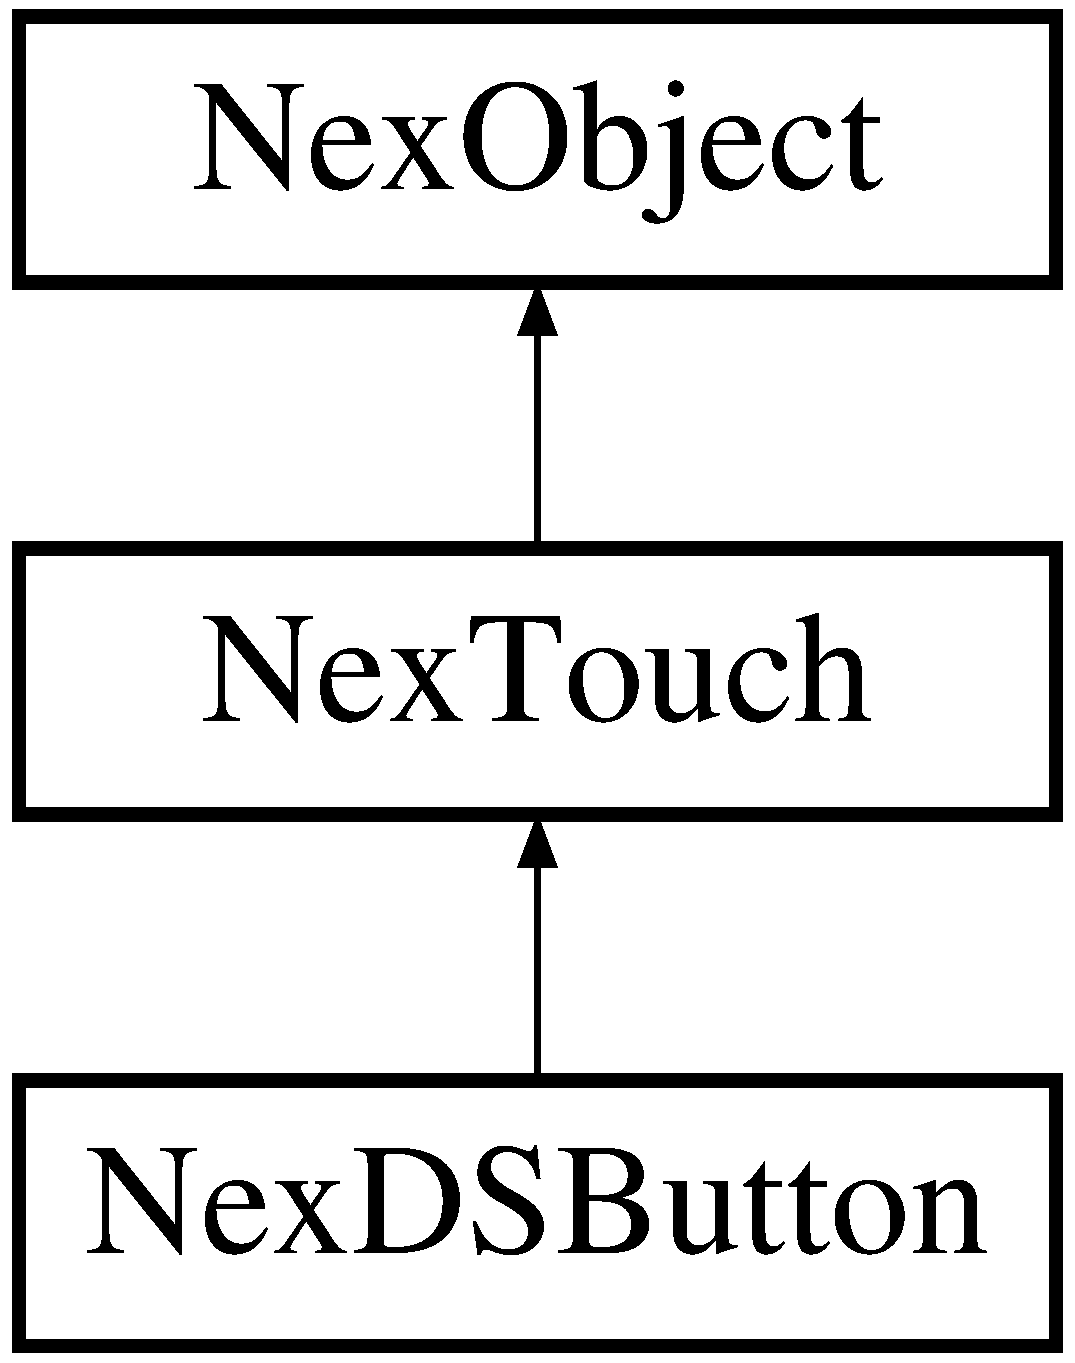
\includegraphics[height=3.000000cm]{class_nex_d_s_button}
\end{center}
\end{figure}
\subsection*{Public Member Functions}
\begin{DoxyCompactItemize}
\item 
\hyperlink{class_nex_d_s_button_a226edd2467f2fdf54848f5235b808e2b}{Nex\+D\+S\+Button} (uint8\+\_\+t pid, uint8\+\_\+t cid, const char $\ast$name)
\item 
bool \hyperlink{class_nex_d_s_button_a63e08f9a79f326c47aa66e1d0f9648c8}{get\+Value} (uint32\+\_\+t $\ast$number)
\item 
bool \hyperlink{class_nex_d_s_button_a2f696207609e0f01aadebb8b3826b0fa}{set\+Value} (uint32\+\_\+t number)
\item 
uint16\+\_\+t \hyperlink{class_nex_d_s_button_aff0f17061441139bf8797c78e4911eae}{get\+Text} (char $\ast$buffer, uint16\+\_\+t len)
\item 
bool \hyperlink{class_nex_d_s_button_aa7a83123530f2dbb3e6aa909352da5b2}{set\+Text} (const char $\ast$buffer)
\item 
uint32\+\_\+t \hyperlink{class_nex_d_s_button_a57119c8695b1dc562319b19864b68203}{Get\+\_\+state0\+\_\+color\+\_\+bco0} (uint32\+\_\+t $\ast$number)
\item 
bool \hyperlink{class_nex_d_s_button_a7276699c1ea7fccf4e52ad05443b8191}{Set\+\_\+state0\+\_\+color\+\_\+bco0} (uint32\+\_\+t number)
\item 
uint32\+\_\+t \hyperlink{class_nex_d_s_button_aa4ce6ec7a670af2df6bd5858ea20e430}{Get\+\_\+state1\+\_\+color\+\_\+bco1} (uint32\+\_\+t $\ast$number)
\item 
bool \hyperlink{class_nex_d_s_button_a42f31d9e9612d7f8403dcf46ef5e8f1a}{Set\+\_\+state1\+\_\+color\+\_\+bco1} (uint32\+\_\+t number)
\item 
uint32\+\_\+t \hyperlink{class_nex_d_s_button_a01a5a7238547cd761b69c49f1619f955}{Get\+\_\+font\+\_\+color\+\_\+pco} (uint32\+\_\+t $\ast$number)
\item 
bool \hyperlink{class_nex_d_s_button_a25e696769de8d33a3e49db15e0b55aaa}{Set\+\_\+font\+\_\+color\+\_\+pco} (uint32\+\_\+t number)
\item 
uint32\+\_\+t \hyperlink{class_nex_d_s_button_ae65ba8eab275c097fa1f9e7f8873dc5d}{Get\+\_\+place\+\_\+xcen} (uint32\+\_\+t $\ast$number)
\item 
bool \hyperlink{class_nex_d_s_button_a0bc679dfaca7aa0439f67bb91814f97a}{Set\+\_\+place\+\_\+xcen} (uint32\+\_\+t number)
\item 
uint32\+\_\+t \hyperlink{class_nex_d_s_button_a2b5c825ceaeeaa588b4830da4f154b23}{Get\+\_\+place\+\_\+ycen} (uint32\+\_\+t $\ast$number)
\item 
bool \hyperlink{class_nex_d_s_button_a356b829500f25b3d5050084474da1165}{Set\+\_\+place\+\_\+ycen} (uint32\+\_\+t number)
\item 
uint32\+\_\+t \hyperlink{class_nex_d_s_button_a3010cd4aa559a30088ad9bf987003adc}{get\+Font} (uint32\+\_\+t $\ast$number)
\item 
bool \hyperlink{class_nex_d_s_button_a2ac5df458d5da7ffdc32bc16160472f8}{set\+Font} (uint32\+\_\+t number)
\item 
uint32\+\_\+t \hyperlink{class_nex_d_s_button_aa48f68183cdbb94e376f1ca0367a2f2c}{Get\+\_\+state0\+\_\+crop\+\_\+picc0} (uint32\+\_\+t $\ast$number)
\item 
bool \hyperlink{class_nex_d_s_button_a8a0427fa8a95021452da9af2f0834eee}{Set\+\_\+state0\+\_\+crop\+\_\+picc0} (uint32\+\_\+t number)
\item 
uint32\+\_\+t \hyperlink{class_nex_d_s_button_a9b24e1ec4677bc8ec921ede2e36c4db6}{Get\+\_\+state1\+\_\+crop\+\_\+picc1} (uint32\+\_\+t $\ast$number)
\item 
bool \hyperlink{class_nex_d_s_button_a1cc8c53007bf420a5e02e0c885ab7460}{Set\+\_\+state1\+\_\+crop\+\_\+picc1} (uint32\+\_\+t number)
\item 
uint32\+\_\+t \hyperlink{class_nex_d_s_button_a8382bc9350b8e589d1ae5da684a0e907}{Get\+\_\+state0\+\_\+image\+\_\+pic0} (uint32\+\_\+t $\ast$number)
\item 
bool \hyperlink{class_nex_d_s_button_a24029fce19d9a0f75a6044e7a44bd925}{Set\+\_\+state0\+\_\+image\+\_\+pic0} (uint32\+\_\+t number)
\item 
uint32\+\_\+t \hyperlink{class_nex_d_s_button_ab52951034a07ac78a9bde09c0bae4514}{Get\+\_\+state1\+\_\+image\+\_\+pic1} (uint32\+\_\+t $\ast$number)
\item 
bool \hyperlink{class_nex_d_s_button_a8d8aafa1a4970faed893db0b666e38b0}{Set\+\_\+state1\+\_\+image\+\_\+pic1} (uint32\+\_\+t number)
\end{DoxyCompactItemize}
\subsection*{Additional Inherited Members}


\subsection{Detailed Description}
\hyperlink{class_nex_d_s_button}{Nex\+D\+S\+Button} component.

Commonly, you want to do something after push and pop it. It is recommanded that only call \hyperlink{class_nex_touch_a4da1c4fcdfadb7eabfb9ccaba9ecad11}{Nex\+Touch\+::attach\+Pop} to satisfy your purpose.

\begin{DoxyWarning}{Warning}
Please do not call \hyperlink{class_nex_touch_a685a753aae5eb9fb9866a7807a310132}{Nex\+Touch\+::attach\+Push} on this component, even though you can. 
\end{DoxyWarning}


\subsection{Constructor \& Destructor Documentation}
\hypertarget{class_nex_d_s_button_a226edd2467f2fdf54848f5235b808e2b}{\index{Nex\+D\+S\+Button@{Nex\+D\+S\+Button}!Nex\+D\+S\+Button@{Nex\+D\+S\+Button}}
\index{Nex\+D\+S\+Button@{Nex\+D\+S\+Button}!Nex\+D\+S\+Button@{Nex\+D\+S\+Button}}
\subsubsection[{Nex\+D\+S\+Button}]{\setlength{\rightskip}{0pt plus 5cm}Nex\+D\+S\+Button\+::\+Nex\+D\+S\+Button (
\begin{DoxyParamCaption}
\item[{uint8\+\_\+t}]{pid, }
\item[{uint8\+\_\+t}]{cid, }
\item[{const char $\ast$}]{name}
\end{DoxyParamCaption}
)}}\label{class_nex_d_s_button_a226edd2467f2fdf54848f5235b808e2b}




Constructor.


\begin{DoxyParams}{Parameters}
{\em pid} & -\/ page id. \\
\hline
{\em cid} & -\/ component id. \\
\hline
{\em name} & -\/ pointer to an unique name in range of all components. \\
\hline
\end{DoxyParams}


\subsection{Member Function Documentation}
\hypertarget{class_nex_d_s_button_a01a5a7238547cd761b69c49f1619f955}{\index{Nex\+D\+S\+Button@{Nex\+D\+S\+Button}!Get\+\_\+font\+\_\+color\+\_\+pco@{Get\+\_\+font\+\_\+color\+\_\+pco}}
\index{Get\+\_\+font\+\_\+color\+\_\+pco@{Get\+\_\+font\+\_\+color\+\_\+pco}!Nex\+D\+S\+Button@{Nex\+D\+S\+Button}}
\subsubsection[{Get\+\_\+font\+\_\+color\+\_\+pco}]{\setlength{\rightskip}{0pt plus 5cm}uint32\+\_\+t Nex\+D\+S\+Button\+::\+Get\+\_\+font\+\_\+color\+\_\+pco (
\begin{DoxyParamCaption}
\item[{uint32\+\_\+t $\ast$}]{number}
\end{DoxyParamCaption}
)}}\label{class_nex_d_s_button_a01a5a7238547cd761b69c49f1619f955}
Get pco attribute of component


\begin{DoxyParams}{Parameters}
{\em number} & -\/ buffer storing data retur \\
\hline
\end{DoxyParams}
\begin{DoxyReturn}{Returns}
the length of the data 
\end{DoxyReturn}
\hypertarget{class_nex_d_s_button_ae65ba8eab275c097fa1f9e7f8873dc5d}{\index{Nex\+D\+S\+Button@{Nex\+D\+S\+Button}!Get\+\_\+place\+\_\+xcen@{Get\+\_\+place\+\_\+xcen}}
\index{Get\+\_\+place\+\_\+xcen@{Get\+\_\+place\+\_\+xcen}!Nex\+D\+S\+Button@{Nex\+D\+S\+Button}}
\subsubsection[{Get\+\_\+place\+\_\+xcen}]{\setlength{\rightskip}{0pt plus 5cm}uint32\+\_\+t Nex\+D\+S\+Button\+::\+Get\+\_\+place\+\_\+xcen (
\begin{DoxyParamCaption}
\item[{uint32\+\_\+t $\ast$}]{number}
\end{DoxyParamCaption}
)}}\label{class_nex_d_s_button_ae65ba8eab275c097fa1f9e7f8873dc5d}
Get xcen attribute of component


\begin{DoxyParams}{Parameters}
{\em number} & -\/ buffer storing data retur \\
\hline
\end{DoxyParams}
\begin{DoxyReturn}{Returns}
the length of the data 
\end{DoxyReturn}
\hypertarget{class_nex_d_s_button_a2b5c825ceaeeaa588b4830da4f154b23}{\index{Nex\+D\+S\+Button@{Nex\+D\+S\+Button}!Get\+\_\+place\+\_\+ycen@{Get\+\_\+place\+\_\+ycen}}
\index{Get\+\_\+place\+\_\+ycen@{Get\+\_\+place\+\_\+ycen}!Nex\+D\+S\+Button@{Nex\+D\+S\+Button}}
\subsubsection[{Get\+\_\+place\+\_\+ycen}]{\setlength{\rightskip}{0pt plus 5cm}uint32\+\_\+t Nex\+D\+S\+Button\+::\+Get\+\_\+place\+\_\+ycen (
\begin{DoxyParamCaption}
\item[{uint32\+\_\+t $\ast$}]{number}
\end{DoxyParamCaption}
)}}\label{class_nex_d_s_button_a2b5c825ceaeeaa588b4830da4f154b23}
Get ycen attribute of component


\begin{DoxyParams}{Parameters}
{\em number} & -\/ buffer storing data retur \\
\hline
\end{DoxyParams}
\begin{DoxyReturn}{Returns}
the length of the data 
\end{DoxyReturn}
\hypertarget{class_nex_d_s_button_a57119c8695b1dc562319b19864b68203}{\index{Nex\+D\+S\+Button@{Nex\+D\+S\+Button}!Get\+\_\+state0\+\_\+color\+\_\+bco0@{Get\+\_\+state0\+\_\+color\+\_\+bco0}}
\index{Get\+\_\+state0\+\_\+color\+\_\+bco0@{Get\+\_\+state0\+\_\+color\+\_\+bco0}!Nex\+D\+S\+Button@{Nex\+D\+S\+Button}}
\subsubsection[{Get\+\_\+state0\+\_\+color\+\_\+bco0}]{\setlength{\rightskip}{0pt plus 5cm}uint32\+\_\+t Nex\+D\+S\+Button\+::\+Get\+\_\+state0\+\_\+color\+\_\+bco0 (
\begin{DoxyParamCaption}
\item[{uint32\+\_\+t $\ast$}]{number}
\end{DoxyParamCaption}
)}}\label{class_nex_d_s_button_a57119c8695b1dc562319b19864b68203}
Get bco0 attribute of component


\begin{DoxyParams}{Parameters}
{\em number} & -\/ buffer storing data retur \\
\hline
\end{DoxyParams}
\begin{DoxyReturn}{Returns}
the length of the data 
\end{DoxyReturn}
\hypertarget{class_nex_d_s_button_aa48f68183cdbb94e376f1ca0367a2f2c}{\index{Nex\+D\+S\+Button@{Nex\+D\+S\+Button}!Get\+\_\+state0\+\_\+crop\+\_\+picc0@{Get\+\_\+state0\+\_\+crop\+\_\+picc0}}
\index{Get\+\_\+state0\+\_\+crop\+\_\+picc0@{Get\+\_\+state0\+\_\+crop\+\_\+picc0}!Nex\+D\+S\+Button@{Nex\+D\+S\+Button}}
\subsubsection[{Get\+\_\+state0\+\_\+crop\+\_\+picc0}]{\setlength{\rightskip}{0pt plus 5cm}uint32\+\_\+t Nex\+D\+S\+Button\+::\+Get\+\_\+state0\+\_\+crop\+\_\+picc0 (
\begin{DoxyParamCaption}
\item[{uint32\+\_\+t $\ast$}]{number}
\end{DoxyParamCaption}
)}}\label{class_nex_d_s_button_aa48f68183cdbb94e376f1ca0367a2f2c}
Get picc0 attribute of component


\begin{DoxyParams}{Parameters}
{\em number} & -\/ buffer storing data retur \\
\hline
\end{DoxyParams}
\begin{DoxyReturn}{Returns}
the length of the data 
\end{DoxyReturn}
\hypertarget{class_nex_d_s_button_a8382bc9350b8e589d1ae5da684a0e907}{\index{Nex\+D\+S\+Button@{Nex\+D\+S\+Button}!Get\+\_\+state0\+\_\+image\+\_\+pic0@{Get\+\_\+state0\+\_\+image\+\_\+pic0}}
\index{Get\+\_\+state0\+\_\+image\+\_\+pic0@{Get\+\_\+state0\+\_\+image\+\_\+pic0}!Nex\+D\+S\+Button@{Nex\+D\+S\+Button}}
\subsubsection[{Get\+\_\+state0\+\_\+image\+\_\+pic0}]{\setlength{\rightskip}{0pt plus 5cm}uint32\+\_\+t Nex\+D\+S\+Button\+::\+Get\+\_\+state0\+\_\+image\+\_\+pic0 (
\begin{DoxyParamCaption}
\item[{uint32\+\_\+t $\ast$}]{number}
\end{DoxyParamCaption}
)}}\label{class_nex_d_s_button_a8382bc9350b8e589d1ae5da684a0e907}
Get pic0 attribute of component


\begin{DoxyParams}{Parameters}
{\em number} & -\/ buffer storing data retur \\
\hline
\end{DoxyParams}
\begin{DoxyReturn}{Returns}
the length of the data 
\end{DoxyReturn}
\hypertarget{class_nex_d_s_button_aa4ce6ec7a670af2df6bd5858ea20e430}{\index{Nex\+D\+S\+Button@{Nex\+D\+S\+Button}!Get\+\_\+state1\+\_\+color\+\_\+bco1@{Get\+\_\+state1\+\_\+color\+\_\+bco1}}
\index{Get\+\_\+state1\+\_\+color\+\_\+bco1@{Get\+\_\+state1\+\_\+color\+\_\+bco1}!Nex\+D\+S\+Button@{Nex\+D\+S\+Button}}
\subsubsection[{Get\+\_\+state1\+\_\+color\+\_\+bco1}]{\setlength{\rightskip}{0pt plus 5cm}uint32\+\_\+t Nex\+D\+S\+Button\+::\+Get\+\_\+state1\+\_\+color\+\_\+bco1 (
\begin{DoxyParamCaption}
\item[{uint32\+\_\+t $\ast$}]{number}
\end{DoxyParamCaption}
)}}\label{class_nex_d_s_button_aa4ce6ec7a670af2df6bd5858ea20e430}
Get bco1 attribute of component


\begin{DoxyParams}{Parameters}
{\em number} & -\/ buffer storing data retur \\
\hline
\end{DoxyParams}
\begin{DoxyReturn}{Returns}
the length of the data 
\end{DoxyReturn}
\hypertarget{class_nex_d_s_button_a9b24e1ec4677bc8ec921ede2e36c4db6}{\index{Nex\+D\+S\+Button@{Nex\+D\+S\+Button}!Get\+\_\+state1\+\_\+crop\+\_\+picc1@{Get\+\_\+state1\+\_\+crop\+\_\+picc1}}
\index{Get\+\_\+state1\+\_\+crop\+\_\+picc1@{Get\+\_\+state1\+\_\+crop\+\_\+picc1}!Nex\+D\+S\+Button@{Nex\+D\+S\+Button}}
\subsubsection[{Get\+\_\+state1\+\_\+crop\+\_\+picc1}]{\setlength{\rightskip}{0pt plus 5cm}uint32\+\_\+t Nex\+D\+S\+Button\+::\+Get\+\_\+state1\+\_\+crop\+\_\+picc1 (
\begin{DoxyParamCaption}
\item[{uint32\+\_\+t $\ast$}]{number}
\end{DoxyParamCaption}
)}}\label{class_nex_d_s_button_a9b24e1ec4677bc8ec921ede2e36c4db6}
Get picc1 attribute of component


\begin{DoxyParams}{Parameters}
{\em number} & -\/ buffer storing data retur \\
\hline
\end{DoxyParams}
\begin{DoxyReturn}{Returns}
the length of the data 
\end{DoxyReturn}
\hypertarget{class_nex_d_s_button_ab52951034a07ac78a9bde09c0bae4514}{\index{Nex\+D\+S\+Button@{Nex\+D\+S\+Button}!Get\+\_\+state1\+\_\+image\+\_\+pic1@{Get\+\_\+state1\+\_\+image\+\_\+pic1}}
\index{Get\+\_\+state1\+\_\+image\+\_\+pic1@{Get\+\_\+state1\+\_\+image\+\_\+pic1}!Nex\+D\+S\+Button@{Nex\+D\+S\+Button}}
\subsubsection[{Get\+\_\+state1\+\_\+image\+\_\+pic1}]{\setlength{\rightskip}{0pt plus 5cm}uint32\+\_\+t Nex\+D\+S\+Button\+::\+Get\+\_\+state1\+\_\+image\+\_\+pic1 (
\begin{DoxyParamCaption}
\item[{uint32\+\_\+t $\ast$}]{number}
\end{DoxyParamCaption}
)}}\label{class_nex_d_s_button_ab52951034a07ac78a9bde09c0bae4514}
Get pic1 attribute of component


\begin{DoxyParams}{Parameters}
{\em number} & -\/ buffer storing data retur \\
\hline
\end{DoxyParams}
\begin{DoxyReturn}{Returns}
the length of the data 
\end{DoxyReturn}
\hypertarget{class_nex_d_s_button_a3010cd4aa559a30088ad9bf987003adc}{\index{Nex\+D\+S\+Button@{Nex\+D\+S\+Button}!get\+Font@{get\+Font}}
\index{get\+Font@{get\+Font}!Nex\+D\+S\+Button@{Nex\+D\+S\+Button}}
\subsubsection[{get\+Font}]{\setlength{\rightskip}{0pt plus 5cm}uint32\+\_\+t Nex\+D\+S\+Button\+::get\+Font (
\begin{DoxyParamCaption}
\item[{uint32\+\_\+t $\ast$}]{number}
\end{DoxyParamCaption}
)}}\label{class_nex_d_s_button_a3010cd4aa559a30088ad9bf987003adc}
Get font attribute of component


\begin{DoxyParams}{Parameters}
{\em number} & -\/ buffer storing data retur \\
\hline
\end{DoxyParams}
\begin{DoxyReturn}{Returns}
the length of the data 
\end{DoxyReturn}
\hypertarget{class_nex_d_s_button_aff0f17061441139bf8797c78e4911eae}{\index{Nex\+D\+S\+Button@{Nex\+D\+S\+Button}!get\+Text@{get\+Text}}
\index{get\+Text@{get\+Text}!Nex\+D\+S\+Button@{Nex\+D\+S\+Button}}
\subsubsection[{get\+Text}]{\setlength{\rightskip}{0pt plus 5cm}uint16\+\_\+t Nex\+D\+S\+Button\+::get\+Text (
\begin{DoxyParamCaption}
\item[{char $\ast$}]{buffer, }
\item[{uint16\+\_\+t}]{len}
\end{DoxyParamCaption}
)}}\label{class_nex_d_s_button_aff0f17061441139bf8797c78e4911eae}
Get text attribute of component.


\begin{DoxyParams}{Parameters}
{\em buffer} & -\/ buffer storing text returned. \\
\hline
{\em len} & -\/ length of buffer. \\
\hline
\end{DoxyParams}
\begin{DoxyReturn}{Returns}
The real length of text returned. 
\end{DoxyReturn}
\hypertarget{class_nex_d_s_button_a63e08f9a79f326c47aa66e1d0f9648c8}{\index{Nex\+D\+S\+Button@{Nex\+D\+S\+Button}!get\+Value@{get\+Value}}
\index{get\+Value@{get\+Value}!Nex\+D\+S\+Button@{Nex\+D\+S\+Button}}
\subsubsection[{get\+Value}]{\setlength{\rightskip}{0pt plus 5cm}bool Nex\+D\+S\+Button\+::get\+Value (
\begin{DoxyParamCaption}
\item[{uint32\+\_\+t $\ast$}]{number}
\end{DoxyParamCaption}
)}}\label{class_nex_d_s_button_a63e08f9a79f326c47aa66e1d0f9648c8}
Get number attribute of component.


\begin{DoxyParams}{Parameters}
{\em number} & -\/ buffer storing text returned. \\
\hline
\end{DoxyParams}
\begin{DoxyReturn}{Returns}
The real length of text returned. 
\end{DoxyReturn}
\hypertarget{class_nex_d_s_button_a25e696769de8d33a3e49db15e0b55aaa}{\index{Nex\+D\+S\+Button@{Nex\+D\+S\+Button}!Set\+\_\+font\+\_\+color\+\_\+pco@{Set\+\_\+font\+\_\+color\+\_\+pco}}
\index{Set\+\_\+font\+\_\+color\+\_\+pco@{Set\+\_\+font\+\_\+color\+\_\+pco}!Nex\+D\+S\+Button@{Nex\+D\+S\+Button}}
\subsubsection[{Set\+\_\+font\+\_\+color\+\_\+pco}]{\setlength{\rightskip}{0pt plus 5cm}bool Nex\+D\+S\+Button\+::\+Set\+\_\+font\+\_\+color\+\_\+pco (
\begin{DoxyParamCaption}
\item[{uint32\+\_\+t}]{number}
\end{DoxyParamCaption}
)}}\label{class_nex_d_s_button_a25e696769de8d33a3e49db15e0b55aaa}
Set pco attribute of component


\begin{DoxyParams}{Parameters}
{\em number} & -\/ To set up the data \\
\hline
\end{DoxyParams}
\begin{DoxyReturn}{Returns}
true if success, false for failure 
\end{DoxyReturn}
\hypertarget{class_nex_d_s_button_a0bc679dfaca7aa0439f67bb91814f97a}{\index{Nex\+D\+S\+Button@{Nex\+D\+S\+Button}!Set\+\_\+place\+\_\+xcen@{Set\+\_\+place\+\_\+xcen}}
\index{Set\+\_\+place\+\_\+xcen@{Set\+\_\+place\+\_\+xcen}!Nex\+D\+S\+Button@{Nex\+D\+S\+Button}}
\subsubsection[{Set\+\_\+place\+\_\+xcen}]{\setlength{\rightskip}{0pt plus 5cm}bool Nex\+D\+S\+Button\+::\+Set\+\_\+place\+\_\+xcen (
\begin{DoxyParamCaption}
\item[{uint32\+\_\+t}]{number}
\end{DoxyParamCaption}
)}}\label{class_nex_d_s_button_a0bc679dfaca7aa0439f67bb91814f97a}
Set xcen attribute of component


\begin{DoxyParams}{Parameters}
{\em number} & -\/ To set up the data \\
\hline
\end{DoxyParams}
\begin{DoxyReturn}{Returns}
true if success, false for failure 
\end{DoxyReturn}
\hypertarget{class_nex_d_s_button_a356b829500f25b3d5050084474da1165}{\index{Nex\+D\+S\+Button@{Nex\+D\+S\+Button}!Set\+\_\+place\+\_\+ycen@{Set\+\_\+place\+\_\+ycen}}
\index{Set\+\_\+place\+\_\+ycen@{Set\+\_\+place\+\_\+ycen}!Nex\+D\+S\+Button@{Nex\+D\+S\+Button}}
\subsubsection[{Set\+\_\+place\+\_\+ycen}]{\setlength{\rightskip}{0pt plus 5cm}bool Nex\+D\+S\+Button\+::\+Set\+\_\+place\+\_\+ycen (
\begin{DoxyParamCaption}
\item[{uint32\+\_\+t}]{number}
\end{DoxyParamCaption}
)}}\label{class_nex_d_s_button_a356b829500f25b3d5050084474da1165}
Set ycen attribute of component


\begin{DoxyParams}{Parameters}
{\em number} & -\/ To set up the data \\
\hline
\end{DoxyParams}
\begin{DoxyReturn}{Returns}
true if success, false for failure 
\end{DoxyReturn}
\hypertarget{class_nex_d_s_button_a7276699c1ea7fccf4e52ad05443b8191}{\index{Nex\+D\+S\+Button@{Nex\+D\+S\+Button}!Set\+\_\+state0\+\_\+color\+\_\+bco0@{Set\+\_\+state0\+\_\+color\+\_\+bco0}}
\index{Set\+\_\+state0\+\_\+color\+\_\+bco0@{Set\+\_\+state0\+\_\+color\+\_\+bco0}!Nex\+D\+S\+Button@{Nex\+D\+S\+Button}}
\subsubsection[{Set\+\_\+state0\+\_\+color\+\_\+bco0}]{\setlength{\rightskip}{0pt plus 5cm}bool Nex\+D\+S\+Button\+::\+Set\+\_\+state0\+\_\+color\+\_\+bco0 (
\begin{DoxyParamCaption}
\item[{uint32\+\_\+t}]{number}
\end{DoxyParamCaption}
)}}\label{class_nex_d_s_button_a7276699c1ea7fccf4e52ad05443b8191}
Set bco0 attribute of component


\begin{DoxyParams}{Parameters}
{\em number} & -\/ To set up the data \\
\hline
\end{DoxyParams}
\begin{DoxyReturn}{Returns}
true if success, false for failure 
\end{DoxyReturn}
\hypertarget{class_nex_d_s_button_a8a0427fa8a95021452da9af2f0834eee}{\index{Nex\+D\+S\+Button@{Nex\+D\+S\+Button}!Set\+\_\+state0\+\_\+crop\+\_\+picc0@{Set\+\_\+state0\+\_\+crop\+\_\+picc0}}
\index{Set\+\_\+state0\+\_\+crop\+\_\+picc0@{Set\+\_\+state0\+\_\+crop\+\_\+picc0}!Nex\+D\+S\+Button@{Nex\+D\+S\+Button}}
\subsubsection[{Set\+\_\+state0\+\_\+crop\+\_\+picc0}]{\setlength{\rightskip}{0pt plus 5cm}bool Nex\+D\+S\+Button\+::\+Set\+\_\+state0\+\_\+crop\+\_\+picc0 (
\begin{DoxyParamCaption}
\item[{uint32\+\_\+t}]{number}
\end{DoxyParamCaption}
)}}\label{class_nex_d_s_button_a8a0427fa8a95021452da9af2f0834eee}
Set picc0 attribute of component


\begin{DoxyParams}{Parameters}
{\em number} & -\/ To set up the data \\
\hline
\end{DoxyParams}
\begin{DoxyReturn}{Returns}
true if success, false for failure 
\end{DoxyReturn}
\hypertarget{class_nex_d_s_button_a24029fce19d9a0f75a6044e7a44bd925}{\index{Nex\+D\+S\+Button@{Nex\+D\+S\+Button}!Set\+\_\+state0\+\_\+image\+\_\+pic0@{Set\+\_\+state0\+\_\+image\+\_\+pic0}}
\index{Set\+\_\+state0\+\_\+image\+\_\+pic0@{Set\+\_\+state0\+\_\+image\+\_\+pic0}!Nex\+D\+S\+Button@{Nex\+D\+S\+Button}}
\subsubsection[{Set\+\_\+state0\+\_\+image\+\_\+pic0}]{\setlength{\rightskip}{0pt plus 5cm}bool Nex\+D\+S\+Button\+::\+Set\+\_\+state0\+\_\+image\+\_\+pic0 (
\begin{DoxyParamCaption}
\item[{uint32\+\_\+t}]{number}
\end{DoxyParamCaption}
)}}\label{class_nex_d_s_button_a24029fce19d9a0f75a6044e7a44bd925}
Set pic0 attribute of component


\begin{DoxyParams}{Parameters}
{\em number} & -\/ To set up the data \\
\hline
\end{DoxyParams}
\begin{DoxyReturn}{Returns}
true if success, false for failure 
\end{DoxyReturn}
\hypertarget{class_nex_d_s_button_a42f31d9e9612d7f8403dcf46ef5e8f1a}{\index{Nex\+D\+S\+Button@{Nex\+D\+S\+Button}!Set\+\_\+state1\+\_\+color\+\_\+bco1@{Set\+\_\+state1\+\_\+color\+\_\+bco1}}
\index{Set\+\_\+state1\+\_\+color\+\_\+bco1@{Set\+\_\+state1\+\_\+color\+\_\+bco1}!Nex\+D\+S\+Button@{Nex\+D\+S\+Button}}
\subsubsection[{Set\+\_\+state1\+\_\+color\+\_\+bco1}]{\setlength{\rightskip}{0pt plus 5cm}bool Nex\+D\+S\+Button\+::\+Set\+\_\+state1\+\_\+color\+\_\+bco1 (
\begin{DoxyParamCaption}
\item[{uint32\+\_\+t}]{number}
\end{DoxyParamCaption}
)}}\label{class_nex_d_s_button_a42f31d9e9612d7f8403dcf46ef5e8f1a}
Set bco1 attribute of component


\begin{DoxyParams}{Parameters}
{\em number} & -\/ To set up the data \\
\hline
\end{DoxyParams}
\begin{DoxyReturn}{Returns}
true if success, false for failure 
\end{DoxyReturn}
\hypertarget{class_nex_d_s_button_a1cc8c53007bf420a5e02e0c885ab7460}{\index{Nex\+D\+S\+Button@{Nex\+D\+S\+Button}!Set\+\_\+state1\+\_\+crop\+\_\+picc1@{Set\+\_\+state1\+\_\+crop\+\_\+picc1}}
\index{Set\+\_\+state1\+\_\+crop\+\_\+picc1@{Set\+\_\+state1\+\_\+crop\+\_\+picc1}!Nex\+D\+S\+Button@{Nex\+D\+S\+Button}}
\subsubsection[{Set\+\_\+state1\+\_\+crop\+\_\+picc1}]{\setlength{\rightskip}{0pt plus 5cm}bool Nex\+D\+S\+Button\+::\+Set\+\_\+state1\+\_\+crop\+\_\+picc1 (
\begin{DoxyParamCaption}
\item[{uint32\+\_\+t}]{number}
\end{DoxyParamCaption}
)}}\label{class_nex_d_s_button_a1cc8c53007bf420a5e02e0c885ab7460}
Set picc1 attribute of component


\begin{DoxyParams}{Parameters}
{\em number} & -\/ To set up the data \\
\hline
\end{DoxyParams}
\begin{DoxyReturn}{Returns}
true if success, false for failure 
\end{DoxyReturn}
\hypertarget{class_nex_d_s_button_a8d8aafa1a4970faed893db0b666e38b0}{\index{Nex\+D\+S\+Button@{Nex\+D\+S\+Button}!Set\+\_\+state1\+\_\+image\+\_\+pic1@{Set\+\_\+state1\+\_\+image\+\_\+pic1}}
\index{Set\+\_\+state1\+\_\+image\+\_\+pic1@{Set\+\_\+state1\+\_\+image\+\_\+pic1}!Nex\+D\+S\+Button@{Nex\+D\+S\+Button}}
\subsubsection[{Set\+\_\+state1\+\_\+image\+\_\+pic1}]{\setlength{\rightskip}{0pt plus 5cm}bool Nex\+D\+S\+Button\+::\+Set\+\_\+state1\+\_\+image\+\_\+pic1 (
\begin{DoxyParamCaption}
\item[{uint32\+\_\+t}]{number}
\end{DoxyParamCaption}
)}}\label{class_nex_d_s_button_a8d8aafa1a4970faed893db0b666e38b0}
Set pic1 attribute of component


\begin{DoxyParams}{Parameters}
{\em number} & -\/ To set up the data \\
\hline
\end{DoxyParams}
\begin{DoxyReturn}{Returns}
true if success, false for failure 
\end{DoxyReturn}
\hypertarget{class_nex_d_s_button_a2ac5df458d5da7ffdc32bc16160472f8}{\index{Nex\+D\+S\+Button@{Nex\+D\+S\+Button}!set\+Font@{set\+Font}}
\index{set\+Font@{set\+Font}!Nex\+D\+S\+Button@{Nex\+D\+S\+Button}}
\subsubsection[{set\+Font}]{\setlength{\rightskip}{0pt plus 5cm}bool Nex\+D\+S\+Button\+::set\+Font (
\begin{DoxyParamCaption}
\item[{uint32\+\_\+t}]{number}
\end{DoxyParamCaption}
)}}\label{class_nex_d_s_button_a2ac5df458d5da7ffdc32bc16160472f8}
Set font attribute of component


\begin{DoxyParams}{Parameters}
{\em number} & -\/ To set up the data \\
\hline
\end{DoxyParams}
\begin{DoxyReturn}{Returns}
true if success, false for failure 
\end{DoxyReturn}
\hypertarget{class_nex_d_s_button_aa7a83123530f2dbb3e6aa909352da5b2}{\index{Nex\+D\+S\+Button@{Nex\+D\+S\+Button}!set\+Text@{set\+Text}}
\index{set\+Text@{set\+Text}!Nex\+D\+S\+Button@{Nex\+D\+S\+Button}}
\subsubsection[{set\+Text}]{\setlength{\rightskip}{0pt plus 5cm}bool Nex\+D\+S\+Button\+::set\+Text (
\begin{DoxyParamCaption}
\item[{const char $\ast$}]{buffer}
\end{DoxyParamCaption}
)}}\label{class_nex_d_s_button_aa7a83123530f2dbb3e6aa909352da5b2}
Set text attribute of component.


\begin{DoxyParams}{Parameters}
{\em buffer} & -\/ text buffer terminated with '\textbackslash{}0'. \\
\hline
\end{DoxyParams}
\begin{DoxyReturn}{Returns}
true if success, false for failure. 
\end{DoxyReturn}
\hypertarget{class_nex_d_s_button_a2f696207609e0f01aadebb8b3826b0fa}{\index{Nex\+D\+S\+Button@{Nex\+D\+S\+Button}!set\+Value@{set\+Value}}
\index{set\+Value@{set\+Value}!Nex\+D\+S\+Button@{Nex\+D\+S\+Button}}
\subsubsection[{set\+Value}]{\setlength{\rightskip}{0pt plus 5cm}bool Nex\+D\+S\+Button\+::set\+Value (
\begin{DoxyParamCaption}
\item[{uint32\+\_\+t}]{number}
\end{DoxyParamCaption}
)}}\label{class_nex_d_s_button_a2f696207609e0f01aadebb8b3826b0fa}
Set number attribute of component.


\begin{DoxyParams}{Parameters}
{\em number} & -\/ number buffer. \\
\hline
\end{DoxyParams}
\begin{DoxyReturn}{Returns}
true if success, false for failure. 
\end{DoxyReturn}


The documentation for this class was generated from the following files\+:\begin{DoxyCompactItemize}
\item 
\hyperlink{_nex_dual_state_button_8h}{Nex\+Dual\+State\+Button.\+h}\item 
\hyperlink{_nex_dual_state_button_8cpp}{Nex\+Dual\+State\+Button.\+cpp}\end{DoxyCompactItemize}

\hypertarget{class_nex_gauge}{\section{Nex\+Gauge Class Reference}
\label{class_nex_gauge}\index{Nex\+Gauge@{Nex\+Gauge}}
}


{\ttfamily \#include $<$Nex\+Gauge.\+h$>$}

Inheritance diagram for Nex\+Gauge\+:\begin{figure}[H]
\begin{center}
\leavevmode
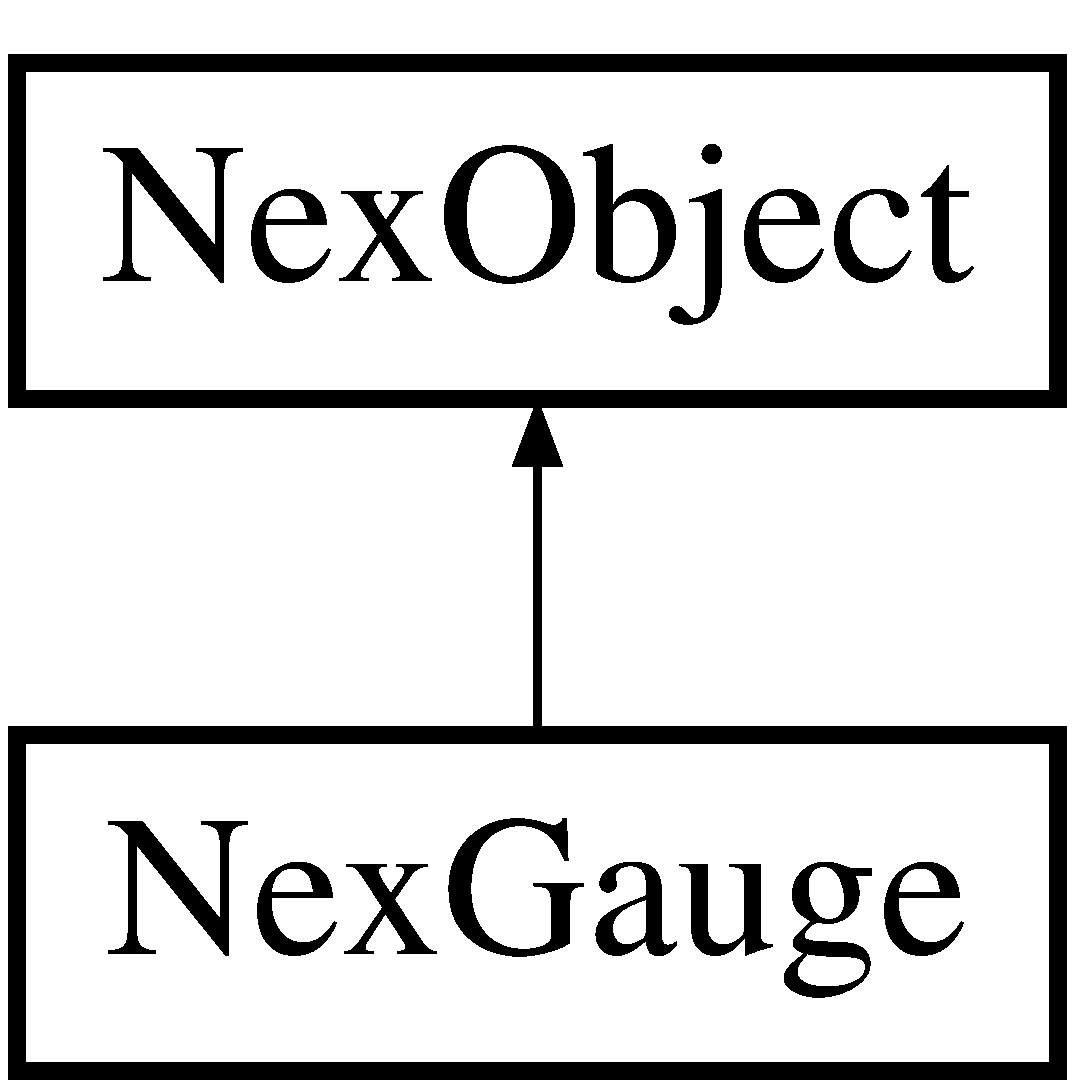
\includegraphics[height=2.000000cm]{class_nex_gauge}
\end{center}
\end{figure}
\subsection*{Public Member Functions}
\begin{DoxyCompactItemize}
\item 
\hyperlink{class_nex_gauge_ac79040067d42f7f1ba16cc4a1dfd8b9b}{Nex\+Gauge} (uint8\+\_\+t pid, uint8\+\_\+t cid, const char $\ast$name)
\item 
bool \hyperlink{class_nex_gauge_aeea8933513ebba11584ad97f8c8b5e69}{get\+Value} (uint32\+\_\+t $\ast$number)
\item 
bool \hyperlink{class_nex_gauge_a448ce9ad69f54c156c325d578a96b765}{set\+Value} (uint32\+\_\+t number)
\item 
uint32\+\_\+t \hyperlink{class_nex_gauge_a03a6441159939961b64728dded177e92}{Get\+\_\+background\+\_\+color\+\_\+bco} (uint32\+\_\+t $\ast$number)
\item 
bool \hyperlink{class_nex_gauge_a2d2fe2d81da81e14a66260c501d644b3}{Set\+\_\+background\+\_\+color\+\_\+bco} (uint32\+\_\+t number)
\item 
uint32\+\_\+t \hyperlink{class_nex_gauge_a830152d58485d55f475376261d52ff62}{Get\+\_\+font\+\_\+color\+\_\+pco} (uint32\+\_\+t $\ast$number)
\item 
bool \hyperlink{class_nex_gauge_ace00cba20b5cf5e1374c1a57bbf9a5f5}{Set\+\_\+font\+\_\+color\+\_\+pco} (uint32\+\_\+t number)
\item 
uint32\+\_\+t \hyperlink{class_nex_gauge_a50b4daf1b8dfb3cc5c329a3664341e11}{Get\+\_\+pointer\+\_\+thickness\+\_\+wid} (uint32\+\_\+t $\ast$number)
\item 
bool \hyperlink{class_nex_gauge_adacdbcb25fdf45654ebc88f572e3bce9}{Set\+\_\+pointer\+\_\+thickness\+\_\+wid} (uint32\+\_\+t number)
\item 
uint32\+\_\+t \hyperlink{class_nex_gauge_a0a6b394a16b03beb6046ec3795d409fe}{Get\+\_\+background\+\_\+cropi\+\_\+picc} (uint32\+\_\+t $\ast$number)
\item 
bool \hyperlink{class_nex_gauge_a223fa8a91a87439047f22ca1c33660df}{Set\+\_\+background\+\_\+crop\+\_\+picc} (uint32\+\_\+t number)
\end{DoxyCompactItemize}
\subsection*{Additional Inherited Members}


\subsection{Detailed Description}
\hyperlink{class_nex_gauge}{Nex\+Gauge} component. 

\subsection{Constructor \& Destructor Documentation}
\hypertarget{class_nex_gauge_ac79040067d42f7f1ba16cc4a1dfd8b9b}{\index{Nex\+Gauge@{Nex\+Gauge}!Nex\+Gauge@{Nex\+Gauge}}
\index{Nex\+Gauge@{Nex\+Gauge}!Nex\+Gauge@{Nex\+Gauge}}
\subsubsection[{Nex\+Gauge}]{\setlength{\rightskip}{0pt plus 5cm}Nex\+Gauge\+::\+Nex\+Gauge (
\begin{DoxyParamCaption}
\item[{uint8\+\_\+t}]{pid, }
\item[{uint8\+\_\+t}]{cid, }
\item[{const char $\ast$}]{name}
\end{DoxyParamCaption}
)}}\label{class_nex_gauge_ac79040067d42f7f1ba16cc4a1dfd8b9b}




Constructor.


\begin{DoxyParams}{Parameters}
{\em pid} & -\/ page id. \\
\hline
{\em cid} & -\/ component id. \\
\hline
{\em name} & -\/ pointer to an unique name in range of all components. \\
\hline
\end{DoxyParams}


\subsection{Member Function Documentation}
\hypertarget{class_nex_gauge_a03a6441159939961b64728dded177e92}{\index{Nex\+Gauge@{Nex\+Gauge}!Get\+\_\+background\+\_\+color\+\_\+bco@{Get\+\_\+background\+\_\+color\+\_\+bco}}
\index{Get\+\_\+background\+\_\+color\+\_\+bco@{Get\+\_\+background\+\_\+color\+\_\+bco}!Nex\+Gauge@{Nex\+Gauge}}
\subsubsection[{Get\+\_\+background\+\_\+color\+\_\+bco}]{\setlength{\rightskip}{0pt plus 5cm}uint32\+\_\+t Nex\+Gauge\+::\+Get\+\_\+background\+\_\+color\+\_\+bco (
\begin{DoxyParamCaption}
\item[{uint32\+\_\+t $\ast$}]{number}
\end{DoxyParamCaption}
)}}\label{class_nex_gauge_a03a6441159939961b64728dded177e92}
Get bco attribute of component


\begin{DoxyParams}{Parameters}
{\em number} & -\/ buffer storing data retur \\
\hline
\end{DoxyParams}
\begin{DoxyReturn}{Returns}
the length of the data 
\end{DoxyReturn}
\hypertarget{class_nex_gauge_a0a6b394a16b03beb6046ec3795d409fe}{\index{Nex\+Gauge@{Nex\+Gauge}!Get\+\_\+background\+\_\+cropi\+\_\+picc@{Get\+\_\+background\+\_\+cropi\+\_\+picc}}
\index{Get\+\_\+background\+\_\+cropi\+\_\+picc@{Get\+\_\+background\+\_\+cropi\+\_\+picc}!Nex\+Gauge@{Nex\+Gauge}}
\subsubsection[{Get\+\_\+background\+\_\+cropi\+\_\+picc}]{\setlength{\rightskip}{0pt plus 5cm}uint32\+\_\+t Nex\+Gauge\+::\+Get\+\_\+background\+\_\+cropi\+\_\+picc (
\begin{DoxyParamCaption}
\item[{uint32\+\_\+t $\ast$}]{number}
\end{DoxyParamCaption}
)}}\label{class_nex_gauge_a0a6b394a16b03beb6046ec3795d409fe}
Get picc attribute of component


\begin{DoxyParams}{Parameters}
{\em number} & -\/ buffer storing data retur \\
\hline
\end{DoxyParams}
\begin{DoxyReturn}{Returns}
the length of the data 
\end{DoxyReturn}
\hypertarget{class_nex_gauge_a830152d58485d55f475376261d52ff62}{\index{Nex\+Gauge@{Nex\+Gauge}!Get\+\_\+font\+\_\+color\+\_\+pco@{Get\+\_\+font\+\_\+color\+\_\+pco}}
\index{Get\+\_\+font\+\_\+color\+\_\+pco@{Get\+\_\+font\+\_\+color\+\_\+pco}!Nex\+Gauge@{Nex\+Gauge}}
\subsubsection[{Get\+\_\+font\+\_\+color\+\_\+pco}]{\setlength{\rightskip}{0pt plus 5cm}uint32\+\_\+t Nex\+Gauge\+::\+Get\+\_\+font\+\_\+color\+\_\+pco (
\begin{DoxyParamCaption}
\item[{uint32\+\_\+t $\ast$}]{number}
\end{DoxyParamCaption}
)}}\label{class_nex_gauge_a830152d58485d55f475376261d52ff62}
Get pco attribute of component


\begin{DoxyParams}{Parameters}
{\em number} & -\/ buffer storing data retur \\
\hline
\end{DoxyParams}
\begin{DoxyReturn}{Returns}
the length of the data 
\end{DoxyReturn}
\hypertarget{class_nex_gauge_a50b4daf1b8dfb3cc5c329a3664341e11}{\index{Nex\+Gauge@{Nex\+Gauge}!Get\+\_\+pointer\+\_\+thickness\+\_\+wid@{Get\+\_\+pointer\+\_\+thickness\+\_\+wid}}
\index{Get\+\_\+pointer\+\_\+thickness\+\_\+wid@{Get\+\_\+pointer\+\_\+thickness\+\_\+wid}!Nex\+Gauge@{Nex\+Gauge}}
\subsubsection[{Get\+\_\+pointer\+\_\+thickness\+\_\+wid}]{\setlength{\rightskip}{0pt plus 5cm}uint32\+\_\+t Nex\+Gauge\+::\+Get\+\_\+pointer\+\_\+thickness\+\_\+wid (
\begin{DoxyParamCaption}
\item[{uint32\+\_\+t $\ast$}]{number}
\end{DoxyParamCaption}
)}}\label{class_nex_gauge_a50b4daf1b8dfb3cc5c329a3664341e11}
Get wid attribute of component


\begin{DoxyParams}{Parameters}
{\em number} & -\/ buffer storing data retur \\
\hline
\end{DoxyParams}
\begin{DoxyReturn}{Returns}
the length of the data 
\end{DoxyReturn}
\hypertarget{class_nex_gauge_aeea8933513ebba11584ad97f8c8b5e69}{\index{Nex\+Gauge@{Nex\+Gauge}!get\+Value@{get\+Value}}
\index{get\+Value@{get\+Value}!Nex\+Gauge@{Nex\+Gauge}}
\subsubsection[{get\+Value}]{\setlength{\rightskip}{0pt plus 5cm}bool Nex\+Gauge\+::get\+Value (
\begin{DoxyParamCaption}
\item[{uint32\+\_\+t $\ast$}]{number}
\end{DoxyParamCaption}
)}}\label{class_nex_gauge_aeea8933513ebba11584ad97f8c8b5e69}
Get the value of gauge.


\begin{DoxyParams}{Parameters}
{\em number} & -\/ an output parameter to save gauge's value.\\
\hline
\end{DoxyParams}

\begin{DoxyRetVals}{Return values}
{\em true} & -\/ success. \\
\hline
{\em false} & -\/ failed. \\
\hline
\end{DoxyRetVals}
\hypertarget{class_nex_gauge_a2d2fe2d81da81e14a66260c501d644b3}{\index{Nex\+Gauge@{Nex\+Gauge}!Set\+\_\+background\+\_\+color\+\_\+bco@{Set\+\_\+background\+\_\+color\+\_\+bco}}
\index{Set\+\_\+background\+\_\+color\+\_\+bco@{Set\+\_\+background\+\_\+color\+\_\+bco}!Nex\+Gauge@{Nex\+Gauge}}
\subsubsection[{Set\+\_\+background\+\_\+color\+\_\+bco}]{\setlength{\rightskip}{0pt plus 5cm}bool Nex\+Gauge\+::\+Set\+\_\+background\+\_\+color\+\_\+bco (
\begin{DoxyParamCaption}
\item[{uint32\+\_\+t}]{number}
\end{DoxyParamCaption}
)}}\label{class_nex_gauge_a2d2fe2d81da81e14a66260c501d644b3}
Set bco attribute of component


\begin{DoxyParams}{Parameters}
{\em number} & -\/ To set up the data \\
\hline
\end{DoxyParams}
\begin{DoxyReturn}{Returns}
true if success, false for failure 
\end{DoxyReturn}
\hypertarget{class_nex_gauge_a223fa8a91a87439047f22ca1c33660df}{\index{Nex\+Gauge@{Nex\+Gauge}!Set\+\_\+background\+\_\+crop\+\_\+picc@{Set\+\_\+background\+\_\+crop\+\_\+picc}}
\index{Set\+\_\+background\+\_\+crop\+\_\+picc@{Set\+\_\+background\+\_\+crop\+\_\+picc}!Nex\+Gauge@{Nex\+Gauge}}
\subsubsection[{Set\+\_\+background\+\_\+crop\+\_\+picc}]{\setlength{\rightskip}{0pt plus 5cm}bool Nex\+Gauge\+::\+Set\+\_\+background\+\_\+crop\+\_\+picc (
\begin{DoxyParamCaption}
\item[{uint32\+\_\+t}]{number}
\end{DoxyParamCaption}
)}}\label{class_nex_gauge_a223fa8a91a87439047f22ca1c33660df}
Set picc attribute of component


\begin{DoxyParams}{Parameters}
{\em number} & -\/ To set up the data \\
\hline
\end{DoxyParams}
\begin{DoxyReturn}{Returns}
true if success, false for failure 
\end{DoxyReturn}
\hypertarget{class_nex_gauge_ace00cba20b5cf5e1374c1a57bbf9a5f5}{\index{Nex\+Gauge@{Nex\+Gauge}!Set\+\_\+font\+\_\+color\+\_\+pco@{Set\+\_\+font\+\_\+color\+\_\+pco}}
\index{Set\+\_\+font\+\_\+color\+\_\+pco@{Set\+\_\+font\+\_\+color\+\_\+pco}!Nex\+Gauge@{Nex\+Gauge}}
\subsubsection[{Set\+\_\+font\+\_\+color\+\_\+pco}]{\setlength{\rightskip}{0pt plus 5cm}bool Nex\+Gauge\+::\+Set\+\_\+font\+\_\+color\+\_\+pco (
\begin{DoxyParamCaption}
\item[{uint32\+\_\+t}]{number}
\end{DoxyParamCaption}
)}}\label{class_nex_gauge_ace00cba20b5cf5e1374c1a57bbf9a5f5}
Set pco attribute of component


\begin{DoxyParams}{Parameters}
{\em number} & -\/ To set up the data \\
\hline
\end{DoxyParams}
\begin{DoxyReturn}{Returns}
true if success, false for failure 
\end{DoxyReturn}
\hypertarget{class_nex_gauge_adacdbcb25fdf45654ebc88f572e3bce9}{\index{Nex\+Gauge@{Nex\+Gauge}!Set\+\_\+pointer\+\_\+thickness\+\_\+wid@{Set\+\_\+pointer\+\_\+thickness\+\_\+wid}}
\index{Set\+\_\+pointer\+\_\+thickness\+\_\+wid@{Set\+\_\+pointer\+\_\+thickness\+\_\+wid}!Nex\+Gauge@{Nex\+Gauge}}
\subsubsection[{Set\+\_\+pointer\+\_\+thickness\+\_\+wid}]{\setlength{\rightskip}{0pt plus 5cm}bool Nex\+Gauge\+::\+Set\+\_\+pointer\+\_\+thickness\+\_\+wid (
\begin{DoxyParamCaption}
\item[{uint32\+\_\+t}]{number}
\end{DoxyParamCaption}
)}}\label{class_nex_gauge_adacdbcb25fdf45654ebc88f572e3bce9}
Set wid attribute of component


\begin{DoxyParams}{Parameters}
{\em number} & -\/ To set up the data \\
\hline
\end{DoxyParams}
\begin{DoxyReturn}{Returns}
true if success, false for failure 
\end{DoxyReturn}
\hypertarget{class_nex_gauge_a448ce9ad69f54c156c325d578a96b765}{\index{Nex\+Gauge@{Nex\+Gauge}!set\+Value@{set\+Value}}
\index{set\+Value@{set\+Value}!Nex\+Gauge@{Nex\+Gauge}}
\subsubsection[{set\+Value}]{\setlength{\rightskip}{0pt plus 5cm}bool Nex\+Gauge\+::set\+Value (
\begin{DoxyParamCaption}
\item[{uint32\+\_\+t}]{number}
\end{DoxyParamCaption}
)}}\label{class_nex_gauge_a448ce9ad69f54c156c325d578a96b765}
Set the value of gauge.


\begin{DoxyParams}{Parameters}
{\em number} & -\/ the value of gauge.\\
\hline
\end{DoxyParams}

\begin{DoxyRetVals}{Return values}
{\em true} & -\/ success. \\
\hline
{\em false} & -\/ failed. \\
\hline
\end{DoxyRetVals}


The documentation for this class was generated from the following files\+:\begin{DoxyCompactItemize}
\item 
\hyperlink{_nex_gauge_8h}{Nex\+Gauge.\+h}\item 
\hyperlink{_nex_gauge_8cpp}{Nex\+Gauge.\+cpp}\end{DoxyCompactItemize}

\hypertarget{class_nex_gpio}{\section{Nex\+Gpio Class Reference}
\label{class_nex_gpio}\index{Nex\+Gpio@{Nex\+Gpio}}
}
\subsection*{Public Member Functions}
\begin{DoxyCompactItemize}
\item 
bool \hyperlink{class_nex_gpio_adbe08eb11827d75c6b2e9c935d9da19a}{pin\+\_\+mode} (uint32\+\_\+t port, uint32\+\_\+t mode, uint32\+\_\+t control\+\_\+id)
\item 
bool \hyperlink{class_nex_gpio_aaea4cb428fa0a2e26927073c20ed64ac}{digital\+\_\+write} (uint32\+\_\+t port, uint32\+\_\+t value)
\item 
uint32\+\_\+t \hyperlink{class_nex_gpio_a36386b97898f0960abda51c6010378eb}{digital\+\_\+read} (uint32\+\_\+t port)
\item 
bool \hyperlink{class_nex_gpio_af21eb91b041d149193bc716202d4a462}{analog\+\_\+write} (uint32\+\_\+t port, uint32\+\_\+t value)
\item 
bool \hyperlink{class_nex_gpio_a62c2cb633e321ef2273eb3a7af6a5b47}{set\+\_\+pwmfreq} (uint32\+\_\+t value)
\item 
uint32\+\_\+t \hyperlink{class_nex_gpio_a8fca87ac0cdfbc8a62dec807b949c36d}{get\+\_\+pwmfreq} (uint32\+\_\+t $\ast$number)
\end{DoxyCompactItemize}


\subsection{Member Function Documentation}
\hypertarget{class_nex_gpio_af21eb91b041d149193bc716202d4a462}{\index{Nex\+Gpio@{Nex\+Gpio}!analog\+\_\+write@{analog\+\_\+write}}
\index{analog\+\_\+write@{analog\+\_\+write}!Nex\+Gpio@{Nex\+Gpio}}
\subsubsection[{analog\+\_\+write}]{\setlength{\rightskip}{0pt plus 5cm}bool Nex\+Gpio\+::analog\+\_\+write (
\begin{DoxyParamCaption}
\item[{uint32\+\_\+t}]{port, }
\item[{uint32\+\_\+t}]{value}
\end{DoxyParamCaption}
)}}\label{class_nex_gpio_af21eb91b041d149193bc716202d4a462}
writes an analog value (P\+W\+M wave) to a pin


\begin{DoxyParams}{Parameters}
{\em port} & -\/ the gpio port number \\
\hline
{\em value} & -\/ the duty cycle\+: between 0 (always off) and 100 (always on). \\
\hline
\end{DoxyParams}
\begin{DoxyReturn}{Returns}
true if success, false for failure 
\end{DoxyReturn}
\hypertarget{class_nex_gpio_a36386b97898f0960abda51c6010378eb}{\index{Nex\+Gpio@{Nex\+Gpio}!digital\+\_\+read@{digital\+\_\+read}}
\index{digital\+\_\+read@{digital\+\_\+read}!Nex\+Gpio@{Nex\+Gpio}}
\subsubsection[{digital\+\_\+read}]{\setlength{\rightskip}{0pt plus 5cm}uint32\+\_\+t Nex\+Gpio\+::digital\+\_\+read (
\begin{DoxyParamCaption}
\item[{uint32\+\_\+t}]{port}
\end{DoxyParamCaption}
)}}\label{class_nex_gpio_a36386b97898f0960abda51c6010378eb}
read a high or a L\+O\+W value to a digital pin


\begin{DoxyParams}{Parameters}
{\em port} & -\/ the gpio port number \\
\hline
\end{DoxyParams}
\begin{DoxyReturn}{Returns}
the value from a specified digital pin, either high or low 
\end{DoxyReturn}
\hypertarget{class_nex_gpio_aaea4cb428fa0a2e26927073c20ed64ac}{\index{Nex\+Gpio@{Nex\+Gpio}!digital\+\_\+write@{digital\+\_\+write}}
\index{digital\+\_\+write@{digital\+\_\+write}!Nex\+Gpio@{Nex\+Gpio}}
\subsubsection[{digital\+\_\+write}]{\setlength{\rightskip}{0pt plus 5cm}bool Nex\+Gpio\+::digital\+\_\+write (
\begin{DoxyParamCaption}
\item[{uint32\+\_\+t}]{port, }
\item[{uint32\+\_\+t}]{value}
\end{DoxyParamCaption}
)}}\label{class_nex_gpio_aaea4cb428fa0a2e26927073c20ed64ac}
write a high or a L\+O\+W value to a digital pin


\begin{DoxyParams}{Parameters}
{\em port} & -\/ the gpio port number \\
\hline
{\em mode} & -\/ the gpio port number \\
\hline
\end{DoxyParams}
\begin{DoxyReturn}{Returns}
true if success, false for failure 
\end{DoxyReturn}
\hypertarget{class_nex_gpio_a8fca87ac0cdfbc8a62dec807b949c36d}{\index{Nex\+Gpio@{Nex\+Gpio}!get\+\_\+pwmfreq@{get\+\_\+pwmfreq}}
\index{get\+\_\+pwmfreq@{get\+\_\+pwmfreq}!Nex\+Gpio@{Nex\+Gpio}}
\subsubsection[{get\+\_\+pwmfreq}]{\setlength{\rightskip}{0pt plus 5cm}uint32\+\_\+t Nex\+Gpio\+::get\+\_\+pwmfreq (
\begin{DoxyParamCaption}
\item[{uint32\+\_\+t $\ast$}]{number}
\end{DoxyParamCaption}
)}}\label{class_nex_gpio_a8fca87ac0cdfbc8a62dec807b949c36d}
read pwm output frequency


\begin{DoxyParams}{Parameters}
{\em number} & -\/ the frequency \\
\hline
\end{DoxyParams}
\begin{DoxyReturn}{Returns}
true if success, false for failure 
\end{DoxyReturn}
\hypertarget{class_nex_gpio_adbe08eb11827d75c6b2e9c935d9da19a}{\index{Nex\+Gpio@{Nex\+Gpio}!pin\+\_\+mode@{pin\+\_\+mode}}
\index{pin\+\_\+mode@{pin\+\_\+mode}!Nex\+Gpio@{Nex\+Gpio}}
\subsubsection[{pin\+\_\+mode}]{\setlength{\rightskip}{0pt plus 5cm}bool Nex\+Gpio\+::pin\+\_\+mode (
\begin{DoxyParamCaption}
\item[{uint32\+\_\+t}]{port, }
\item[{uint32\+\_\+t}]{mode, }
\item[{uint32\+\_\+t}]{control\+\_\+id}
\end{DoxyParamCaption}
)}}\label{class_nex_gpio_adbe08eb11827d75c6b2e9c935d9da19a}
Set gpio mode


\begin{DoxyParams}{Parameters}
{\em port} & -\/ the gpio port number \\
\hline
{\em mode} & -\/ set gpio port mode(0--Pull on the input 1--the control input binding 2--Push-\/pull output 3--pwm output 4--open mode leakage) \\
\hline
{\em control\+\_\+id} & -\/ nextion controls id ,when the modeel is 1 to be valid \\
\hline
\end{DoxyParams}
\begin{DoxyReturn}{Returns}
true if success, false for failure 
\end{DoxyReturn}
\hypertarget{class_nex_gpio_a62c2cb633e321ef2273eb3a7af6a5b47}{\index{Nex\+Gpio@{Nex\+Gpio}!set\+\_\+pwmfreq@{set\+\_\+pwmfreq}}
\index{set\+\_\+pwmfreq@{set\+\_\+pwmfreq}!Nex\+Gpio@{Nex\+Gpio}}
\subsubsection[{set\+\_\+pwmfreq}]{\setlength{\rightskip}{0pt plus 5cm}bool Nex\+Gpio\+::set\+\_\+pwmfreq (
\begin{DoxyParamCaption}
\item[{uint32\+\_\+t}]{value}
\end{DoxyParamCaption}
)}}\label{class_nex_gpio_a62c2cb633e321ef2273eb3a7af6a5b47}
writes pwm output frequency


\begin{DoxyParams}{Parameters}
{\em value} & -\/ the frequency\+: between 1 and 65535 \\
\hline
\end{DoxyParams}
\begin{DoxyReturn}{Returns}
true if success, false for failure 
\end{DoxyReturn}


The documentation for this class was generated from the following files\+:\begin{DoxyCompactItemize}
\item 
Nex\+Gpio.\+h\item 
\hyperlink{_nex_gpio_8cpp}{Nex\+Gpio.\+cpp}\end{DoxyCompactItemize}

\hypertarget{class_nex_hotspot}{\section{Nex\+Hotspot Class Reference}
\label{class_nex_hotspot}\index{Nex\+Hotspot@{Nex\+Hotspot}}
}


{\ttfamily \#include $<$Nex\+Hotspot.\+h$>$}

Inheritance diagram for Nex\+Hotspot\+:\begin{figure}[H]
\begin{center}
\leavevmode
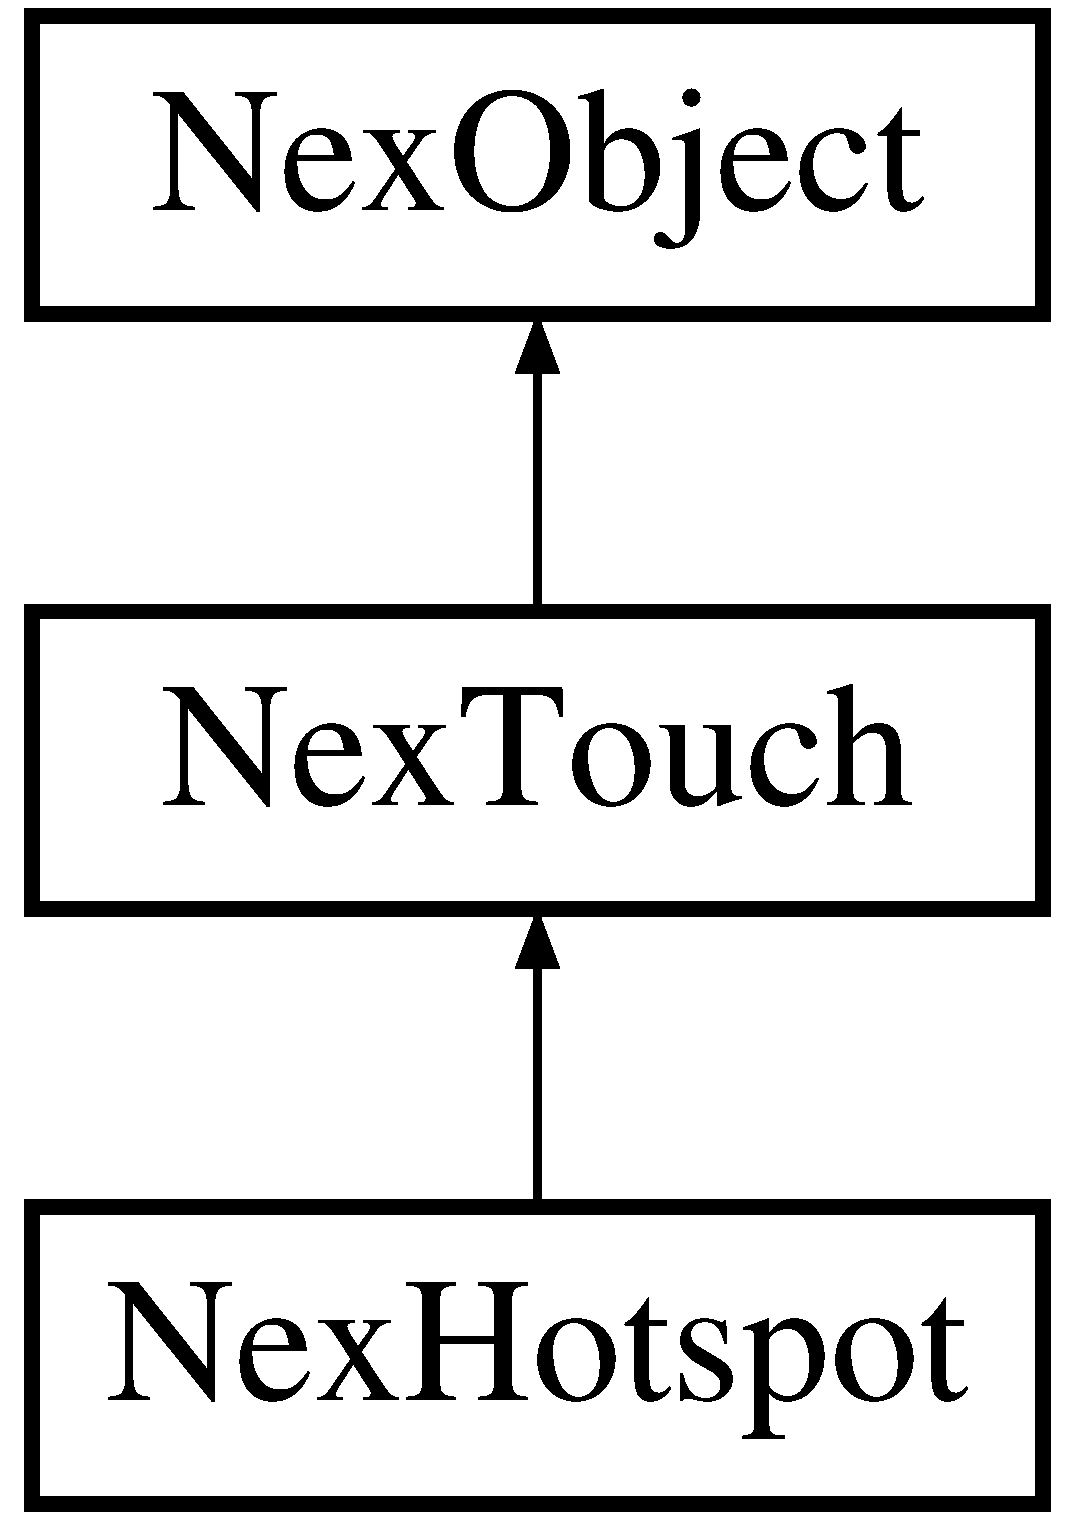
\includegraphics[height=3.000000cm]{class_nex_hotspot}
\end{center}
\end{figure}
\subsection*{Public Member Functions}
\begin{DoxyCompactItemize}
\item 
\hyperlink{class_nex_hotspot_ad2408e74f5445941897702c4c78fddbf}{Nex\+Hotspot} (uint8\+\_\+t pid, uint8\+\_\+t cid, const char $\ast$name)
\end{DoxyCompactItemize}
\subsection*{Additional Inherited Members}


\subsection{Detailed Description}
\hyperlink{class_nex_hotspot}{Nex\+Hotspot} component. 

\subsection{Constructor \& Destructor Documentation}
\hypertarget{class_nex_hotspot_ad2408e74f5445941897702c4c78fddbf}{\index{Nex\+Hotspot@{Nex\+Hotspot}!Nex\+Hotspot@{Nex\+Hotspot}}
\index{Nex\+Hotspot@{Nex\+Hotspot}!Nex\+Hotspot@{Nex\+Hotspot}}
\subsubsection[{Nex\+Hotspot}]{\setlength{\rightskip}{0pt plus 5cm}Nex\+Hotspot\+::\+Nex\+Hotspot (
\begin{DoxyParamCaption}
\item[{uint8\+\_\+t}]{pid, }
\item[{uint8\+\_\+t}]{cid, }
\item[{const char $\ast$}]{name}
\end{DoxyParamCaption}
)}}\label{class_nex_hotspot_ad2408e74f5445941897702c4c78fddbf}




Constructor.


\begin{DoxyParams}{Parameters}
{\em pid} & -\/ page id. \\
\hline
{\em cid} & -\/ component id. \\
\hline
{\em name} & -\/ pointer to an unique name in range of all components. \\
\hline
\end{DoxyParams}


The documentation for this class was generated from the following files\+:\begin{DoxyCompactItemize}
\item 
\hyperlink{_nex_hotspot_8h}{Nex\+Hotspot.\+h}\item 
\hyperlink{_nex_hotspot_8cpp}{Nex\+Hotspot.\+cpp}\end{DoxyCompactItemize}

\hypertarget{class_nex_number}{\section{Nex\+Number Class Reference}
\label{class_nex_number}\index{Nex\+Number@{Nex\+Number}}
}


{\ttfamily \#include $<$Nex\+Number.\+h$>$}

Inheritance diagram for Nex\+Number\+:\begin{figure}[H]
\begin{center}
\leavevmode
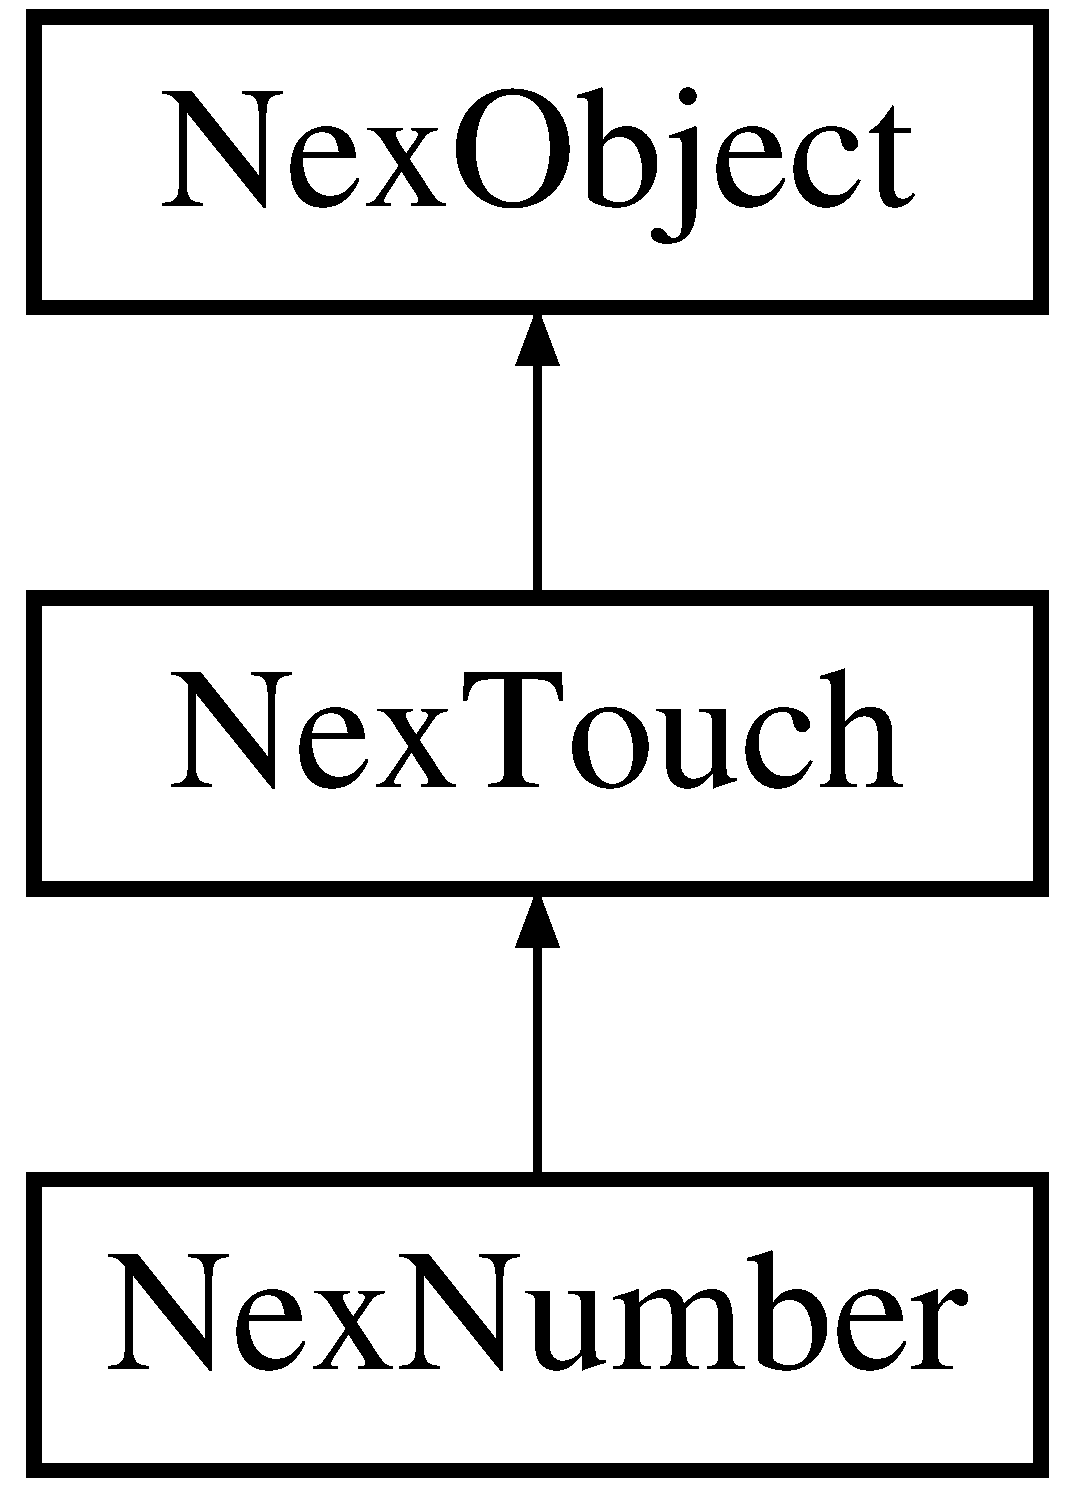
\includegraphics[height=3.000000cm]{class_nex_number}
\end{center}
\end{figure}
\subsection*{Public Member Functions}
\begin{DoxyCompactItemize}
\item 
\hyperlink{class_nex_number_a59c2ed35b787f498e7fbc54eff71d00b}{Nex\+Number} (uint8\+\_\+t pid, uint8\+\_\+t cid, const char $\ast$name)
\item 
bool \hyperlink{class_nex_number_ad184ed818666ec482efddf840185c7b8}{get\+Value} (uint32\+\_\+t $\ast$number)
\item 
bool \hyperlink{class_nex_number_a9cef51f6b76b4ba03a31b2427ffd4526}{set\+Value} (uint32\+\_\+t number)
\item 
uint32\+\_\+t \hyperlink{class_nex_number_aa7ef40e79d89eb0aeebbeb67147a0d20}{Get\+\_\+background\+\_\+color\+\_\+bco} (uint32\+\_\+t $\ast$number)
\item 
bool \hyperlink{class_nex_number_a8168c315e57d9aec3b61ed4febaa6663}{Set\+\_\+background\+\_\+color\+\_\+bco} (uint32\+\_\+t number)
\item 
uint32\+\_\+t \hyperlink{class_nex_number_a7eb3fba2bfa2fff8df8e7e0f633f9cf9}{Get\+\_\+font\+\_\+color\+\_\+pco} (uint32\+\_\+t $\ast$number)
\item 
bool \hyperlink{class_nex_number_ab1836d2d570fca4cd707acecc4b67dea}{Set\+\_\+font\+\_\+color\+\_\+pco} (uint32\+\_\+t number)
\item 
uint32\+\_\+t \hyperlink{class_nex_number_a7ca05534f06911218bae6606ccc355fa}{Get\+\_\+place\+\_\+xcen} (uint32\+\_\+t $\ast$number)
\item 
bool \hyperlink{class_nex_number_a5e58200c740340cc2666e61b6c80e891}{Set\+\_\+place\+\_\+xcen} (uint32\+\_\+t number)
\item 
uint32\+\_\+t \hyperlink{class_nex_number_ac8f0cef0d04e72bb864f6da88f028c9f}{Get\+\_\+place\+\_\+ycen} (uint32\+\_\+t $\ast$number)
\item 
bool \hyperlink{class_nex_number_a05aa6572aabe07b48c1b0675904aaadd}{Set\+\_\+place\+\_\+ycen} (uint32\+\_\+t number)
\item 
uint32\+\_\+t \hyperlink{class_nex_number_a8ccd35555397e828cf8b1f0a8e9ba294}{get\+Font} (uint32\+\_\+t $\ast$number)
\item 
bool \hyperlink{class_nex_number_aed567aef79411c5457c81be272218439}{set\+Font} (uint32\+\_\+t number)
\item 
uint32\+\_\+t \hyperlink{class_nex_number_a0dfc73db91229f114e502bc14084e711}{Get\+\_\+number\+\_\+lenth} (uint32\+\_\+t $\ast$number)
\item 
bool \hyperlink{class_nex_number_a045519a466875775d561e54176c459ad}{Set\+\_\+number\+\_\+lenth} (uint32\+\_\+t number)
\item 
uint32\+\_\+t \hyperlink{class_nex_number_a9772a6717c19c5a03ea0e33ff71492d9}{Get\+\_\+background\+\_\+crop\+\_\+picc} (uint32\+\_\+t $\ast$number)
\item 
bool \hyperlink{class_nex_number_a410bd4092a5874541da654edd86a01eb}{Set\+\_\+background\+\_\+crop\+\_\+picc} (uint32\+\_\+t number)
\item 
uint32\+\_\+t \hyperlink{class_nex_number_a9f235a8929b4f6c282511c04c88216c1}{Get\+\_\+background\+\_\+image\+\_\+pic} (uint32\+\_\+t $\ast$number)
\item 
bool \hyperlink{class_nex_number_aa45acacbde526fce04c699104114d1f1}{Set\+\_\+background\+\_\+image\+\_\+pic} (uint32\+\_\+t number)
\end{DoxyCompactItemize}
\subsection*{Additional Inherited Members}


\subsection{Detailed Description}
\hyperlink{class_nex_number}{Nex\+Number} component. 

\subsection{Constructor \& Destructor Documentation}
\hypertarget{class_nex_number_a59c2ed35b787f498e7fbc54eff71d00b}{\index{Nex\+Number@{Nex\+Number}!Nex\+Number@{Nex\+Number}}
\index{Nex\+Number@{Nex\+Number}!Nex\+Number@{Nex\+Number}}
\subsubsection[{Nex\+Number}]{\setlength{\rightskip}{0pt plus 5cm}Nex\+Number\+::\+Nex\+Number (
\begin{DoxyParamCaption}
\item[{uint8\+\_\+t}]{pid, }
\item[{uint8\+\_\+t}]{cid, }
\item[{const char $\ast$}]{name}
\end{DoxyParamCaption}
)}}\label{class_nex_number_a59c2ed35b787f498e7fbc54eff71d00b}




Constructor.


\begin{DoxyParams}{Parameters}
{\em pid} & -\/ page id. \\
\hline
{\em cid} & -\/ component id. \\
\hline
{\em name} & -\/ pointer to an unique name in range of all components. \\
\hline
\end{DoxyParams}


\subsection{Member Function Documentation}
\hypertarget{class_nex_number_aa7ef40e79d89eb0aeebbeb67147a0d20}{\index{Nex\+Number@{Nex\+Number}!Get\+\_\+background\+\_\+color\+\_\+bco@{Get\+\_\+background\+\_\+color\+\_\+bco}}
\index{Get\+\_\+background\+\_\+color\+\_\+bco@{Get\+\_\+background\+\_\+color\+\_\+bco}!Nex\+Number@{Nex\+Number}}
\subsubsection[{Get\+\_\+background\+\_\+color\+\_\+bco}]{\setlength{\rightskip}{0pt plus 5cm}uint32\+\_\+t Nex\+Number\+::\+Get\+\_\+background\+\_\+color\+\_\+bco (
\begin{DoxyParamCaption}
\item[{uint32\+\_\+t $\ast$}]{number}
\end{DoxyParamCaption}
)}}\label{class_nex_number_aa7ef40e79d89eb0aeebbeb67147a0d20}
Get bco attribute of component


\begin{DoxyParams}{Parameters}
{\em number} & -\/ buffer storing data retur \\
\hline
\end{DoxyParams}
\begin{DoxyReturn}{Returns}
the length of the data 
\end{DoxyReturn}
\hypertarget{class_nex_number_a9772a6717c19c5a03ea0e33ff71492d9}{\index{Nex\+Number@{Nex\+Number}!Get\+\_\+background\+\_\+crop\+\_\+picc@{Get\+\_\+background\+\_\+crop\+\_\+picc}}
\index{Get\+\_\+background\+\_\+crop\+\_\+picc@{Get\+\_\+background\+\_\+crop\+\_\+picc}!Nex\+Number@{Nex\+Number}}
\subsubsection[{Get\+\_\+background\+\_\+crop\+\_\+picc}]{\setlength{\rightskip}{0pt plus 5cm}uint32\+\_\+t Nex\+Number\+::\+Get\+\_\+background\+\_\+crop\+\_\+picc (
\begin{DoxyParamCaption}
\item[{uint32\+\_\+t $\ast$}]{number}
\end{DoxyParamCaption}
)}}\label{class_nex_number_a9772a6717c19c5a03ea0e33ff71492d9}
Get picc attribute of component


\begin{DoxyParams}{Parameters}
{\em number} & -\/ buffer storing data retur \\
\hline
\end{DoxyParams}
\begin{DoxyReturn}{Returns}
the length of the data 
\end{DoxyReturn}
\hypertarget{class_nex_number_a9f235a8929b4f6c282511c04c88216c1}{\index{Nex\+Number@{Nex\+Number}!Get\+\_\+background\+\_\+image\+\_\+pic@{Get\+\_\+background\+\_\+image\+\_\+pic}}
\index{Get\+\_\+background\+\_\+image\+\_\+pic@{Get\+\_\+background\+\_\+image\+\_\+pic}!Nex\+Number@{Nex\+Number}}
\subsubsection[{Get\+\_\+background\+\_\+image\+\_\+pic}]{\setlength{\rightskip}{0pt plus 5cm}uint32\+\_\+t Nex\+Number\+::\+Get\+\_\+background\+\_\+image\+\_\+pic (
\begin{DoxyParamCaption}
\item[{uint32\+\_\+t $\ast$}]{number}
\end{DoxyParamCaption}
)}}\label{class_nex_number_a9f235a8929b4f6c282511c04c88216c1}
Get pic attribute of component


\begin{DoxyParams}{Parameters}
{\em number} & -\/ buffer storing data retur \\
\hline
\end{DoxyParams}
\begin{DoxyReturn}{Returns}
the length of the data 
\end{DoxyReturn}
\hypertarget{class_nex_number_a7eb3fba2bfa2fff8df8e7e0f633f9cf9}{\index{Nex\+Number@{Nex\+Number}!Get\+\_\+font\+\_\+color\+\_\+pco@{Get\+\_\+font\+\_\+color\+\_\+pco}}
\index{Get\+\_\+font\+\_\+color\+\_\+pco@{Get\+\_\+font\+\_\+color\+\_\+pco}!Nex\+Number@{Nex\+Number}}
\subsubsection[{Get\+\_\+font\+\_\+color\+\_\+pco}]{\setlength{\rightskip}{0pt plus 5cm}uint32\+\_\+t Nex\+Number\+::\+Get\+\_\+font\+\_\+color\+\_\+pco (
\begin{DoxyParamCaption}
\item[{uint32\+\_\+t $\ast$}]{number}
\end{DoxyParamCaption}
)}}\label{class_nex_number_a7eb3fba2bfa2fff8df8e7e0f633f9cf9}
Get pco attribute of component


\begin{DoxyParams}{Parameters}
{\em number} & -\/ buffer storing data retur \\
\hline
\end{DoxyParams}
\begin{DoxyReturn}{Returns}
the length of the data 
\end{DoxyReturn}
\hypertarget{class_nex_number_a0dfc73db91229f114e502bc14084e711}{\index{Nex\+Number@{Nex\+Number}!Get\+\_\+number\+\_\+lenth@{Get\+\_\+number\+\_\+lenth}}
\index{Get\+\_\+number\+\_\+lenth@{Get\+\_\+number\+\_\+lenth}!Nex\+Number@{Nex\+Number}}
\subsubsection[{Get\+\_\+number\+\_\+lenth}]{\setlength{\rightskip}{0pt plus 5cm}uint32\+\_\+t Nex\+Number\+::\+Get\+\_\+number\+\_\+lenth (
\begin{DoxyParamCaption}
\item[{uint32\+\_\+t $\ast$}]{number}
\end{DoxyParamCaption}
)}}\label{class_nex_number_a0dfc73db91229f114e502bc14084e711}
Get lenth attribute of component


\begin{DoxyParams}{Parameters}
{\em number} & -\/ buffer storing data retur \\
\hline
\end{DoxyParams}
\begin{DoxyReturn}{Returns}
the length of the data 
\end{DoxyReturn}
\hypertarget{class_nex_number_a7ca05534f06911218bae6606ccc355fa}{\index{Nex\+Number@{Nex\+Number}!Get\+\_\+place\+\_\+xcen@{Get\+\_\+place\+\_\+xcen}}
\index{Get\+\_\+place\+\_\+xcen@{Get\+\_\+place\+\_\+xcen}!Nex\+Number@{Nex\+Number}}
\subsubsection[{Get\+\_\+place\+\_\+xcen}]{\setlength{\rightskip}{0pt plus 5cm}uint32\+\_\+t Nex\+Number\+::\+Get\+\_\+place\+\_\+xcen (
\begin{DoxyParamCaption}
\item[{uint32\+\_\+t $\ast$}]{number}
\end{DoxyParamCaption}
)}}\label{class_nex_number_a7ca05534f06911218bae6606ccc355fa}
Get xcen attribute of component


\begin{DoxyParams}{Parameters}
{\em number} & -\/ buffer storing data retur \\
\hline
\end{DoxyParams}
\begin{DoxyReturn}{Returns}
the length of the data 
\end{DoxyReturn}
\hypertarget{class_nex_number_ac8f0cef0d04e72bb864f6da88f028c9f}{\index{Nex\+Number@{Nex\+Number}!Get\+\_\+place\+\_\+ycen@{Get\+\_\+place\+\_\+ycen}}
\index{Get\+\_\+place\+\_\+ycen@{Get\+\_\+place\+\_\+ycen}!Nex\+Number@{Nex\+Number}}
\subsubsection[{Get\+\_\+place\+\_\+ycen}]{\setlength{\rightskip}{0pt plus 5cm}uint32\+\_\+t Nex\+Number\+::\+Get\+\_\+place\+\_\+ycen (
\begin{DoxyParamCaption}
\item[{uint32\+\_\+t $\ast$}]{number}
\end{DoxyParamCaption}
)}}\label{class_nex_number_ac8f0cef0d04e72bb864f6da88f028c9f}
Get ycen attribute of component


\begin{DoxyParams}{Parameters}
{\em number} & -\/ buffer storing data retur \\
\hline
\end{DoxyParams}
\begin{DoxyReturn}{Returns}
the length of the data 
\end{DoxyReturn}
\hypertarget{class_nex_number_a8ccd35555397e828cf8b1f0a8e9ba294}{\index{Nex\+Number@{Nex\+Number}!get\+Font@{get\+Font}}
\index{get\+Font@{get\+Font}!Nex\+Number@{Nex\+Number}}
\subsubsection[{get\+Font}]{\setlength{\rightskip}{0pt plus 5cm}uint32\+\_\+t Nex\+Number\+::get\+Font (
\begin{DoxyParamCaption}
\item[{uint32\+\_\+t $\ast$}]{number}
\end{DoxyParamCaption}
)}}\label{class_nex_number_a8ccd35555397e828cf8b1f0a8e9ba294}
Get font attribute of component


\begin{DoxyParams}{Parameters}
{\em number} & -\/ buffer storing data retur \\
\hline
\end{DoxyParams}
\begin{DoxyReturn}{Returns}
the length of the data 
\end{DoxyReturn}
\hypertarget{class_nex_number_ad184ed818666ec482efddf840185c7b8}{\index{Nex\+Number@{Nex\+Number}!get\+Value@{get\+Value}}
\index{get\+Value@{get\+Value}!Nex\+Number@{Nex\+Number}}
\subsubsection[{get\+Value}]{\setlength{\rightskip}{0pt plus 5cm}bool Nex\+Number\+::get\+Value (
\begin{DoxyParamCaption}
\item[{uint32\+\_\+t $\ast$}]{number}
\end{DoxyParamCaption}
)}}\label{class_nex_number_ad184ed818666ec482efddf840185c7b8}
Get number attribute of component.


\begin{DoxyParams}{Parameters}
{\em number} & -\/ buffer storing text returned. \\
\hline
\end{DoxyParams}
\begin{DoxyReturn}{Returns}
The real length of text returned. 
\end{DoxyReturn}
\hypertarget{class_nex_number_a8168c315e57d9aec3b61ed4febaa6663}{\index{Nex\+Number@{Nex\+Number}!Set\+\_\+background\+\_\+color\+\_\+bco@{Set\+\_\+background\+\_\+color\+\_\+bco}}
\index{Set\+\_\+background\+\_\+color\+\_\+bco@{Set\+\_\+background\+\_\+color\+\_\+bco}!Nex\+Number@{Nex\+Number}}
\subsubsection[{Set\+\_\+background\+\_\+color\+\_\+bco}]{\setlength{\rightskip}{0pt plus 5cm}bool Nex\+Number\+::\+Set\+\_\+background\+\_\+color\+\_\+bco (
\begin{DoxyParamCaption}
\item[{uint32\+\_\+t}]{number}
\end{DoxyParamCaption}
)}}\label{class_nex_number_a8168c315e57d9aec3b61ed4febaa6663}
Set bco attribute of component


\begin{DoxyParams}{Parameters}
{\em number} & -\/ To set up the data \\
\hline
\end{DoxyParams}
\begin{DoxyReturn}{Returns}
true if success, false for failure 
\end{DoxyReturn}
\hypertarget{class_nex_number_a410bd4092a5874541da654edd86a01eb}{\index{Nex\+Number@{Nex\+Number}!Set\+\_\+background\+\_\+crop\+\_\+picc@{Set\+\_\+background\+\_\+crop\+\_\+picc}}
\index{Set\+\_\+background\+\_\+crop\+\_\+picc@{Set\+\_\+background\+\_\+crop\+\_\+picc}!Nex\+Number@{Nex\+Number}}
\subsubsection[{Set\+\_\+background\+\_\+crop\+\_\+picc}]{\setlength{\rightskip}{0pt plus 5cm}bool Nex\+Number\+::\+Set\+\_\+background\+\_\+crop\+\_\+picc (
\begin{DoxyParamCaption}
\item[{uint32\+\_\+t}]{number}
\end{DoxyParamCaption}
)}}\label{class_nex_number_a410bd4092a5874541da654edd86a01eb}
Set picc attribute of component


\begin{DoxyParams}{Parameters}
{\em number} & -\/ To set up the data \\
\hline
\end{DoxyParams}
\begin{DoxyReturn}{Returns}
true if success, false for failure 
\end{DoxyReturn}
\hypertarget{class_nex_number_aa45acacbde526fce04c699104114d1f1}{\index{Nex\+Number@{Nex\+Number}!Set\+\_\+background\+\_\+image\+\_\+pic@{Set\+\_\+background\+\_\+image\+\_\+pic}}
\index{Set\+\_\+background\+\_\+image\+\_\+pic@{Set\+\_\+background\+\_\+image\+\_\+pic}!Nex\+Number@{Nex\+Number}}
\subsubsection[{Set\+\_\+background\+\_\+image\+\_\+pic}]{\setlength{\rightskip}{0pt plus 5cm}bool Nex\+Number\+::\+Set\+\_\+background\+\_\+image\+\_\+pic (
\begin{DoxyParamCaption}
\item[{uint32\+\_\+t}]{number}
\end{DoxyParamCaption}
)}}\label{class_nex_number_aa45acacbde526fce04c699104114d1f1}
Set pic attribute of component


\begin{DoxyParams}{Parameters}
{\em number} & -\/ To set up the data \\
\hline
\end{DoxyParams}
\begin{DoxyReturn}{Returns}
true if success, false for failure 
\end{DoxyReturn}
\hypertarget{class_nex_number_ab1836d2d570fca4cd707acecc4b67dea}{\index{Nex\+Number@{Nex\+Number}!Set\+\_\+font\+\_\+color\+\_\+pco@{Set\+\_\+font\+\_\+color\+\_\+pco}}
\index{Set\+\_\+font\+\_\+color\+\_\+pco@{Set\+\_\+font\+\_\+color\+\_\+pco}!Nex\+Number@{Nex\+Number}}
\subsubsection[{Set\+\_\+font\+\_\+color\+\_\+pco}]{\setlength{\rightskip}{0pt plus 5cm}bool Nex\+Number\+::\+Set\+\_\+font\+\_\+color\+\_\+pco (
\begin{DoxyParamCaption}
\item[{uint32\+\_\+t}]{number}
\end{DoxyParamCaption}
)}}\label{class_nex_number_ab1836d2d570fca4cd707acecc4b67dea}
Set pco attribute of component


\begin{DoxyParams}{Parameters}
{\em number} & -\/ To set up the data \\
\hline
\end{DoxyParams}
\begin{DoxyReturn}{Returns}
true if success, false for failure 
\end{DoxyReturn}
\hypertarget{class_nex_number_a045519a466875775d561e54176c459ad}{\index{Nex\+Number@{Nex\+Number}!Set\+\_\+number\+\_\+lenth@{Set\+\_\+number\+\_\+lenth}}
\index{Set\+\_\+number\+\_\+lenth@{Set\+\_\+number\+\_\+lenth}!Nex\+Number@{Nex\+Number}}
\subsubsection[{Set\+\_\+number\+\_\+lenth}]{\setlength{\rightskip}{0pt plus 5cm}bool Nex\+Number\+::\+Set\+\_\+number\+\_\+lenth (
\begin{DoxyParamCaption}
\item[{uint32\+\_\+t}]{number}
\end{DoxyParamCaption}
)}}\label{class_nex_number_a045519a466875775d561e54176c459ad}
Set lenth attribute of component


\begin{DoxyParams}{Parameters}
{\em number} & -\/ To set up the data \\
\hline
\end{DoxyParams}
\begin{DoxyReturn}{Returns}
true if success, false for failure 
\end{DoxyReturn}
\hypertarget{class_nex_number_a5e58200c740340cc2666e61b6c80e891}{\index{Nex\+Number@{Nex\+Number}!Set\+\_\+place\+\_\+xcen@{Set\+\_\+place\+\_\+xcen}}
\index{Set\+\_\+place\+\_\+xcen@{Set\+\_\+place\+\_\+xcen}!Nex\+Number@{Nex\+Number}}
\subsubsection[{Set\+\_\+place\+\_\+xcen}]{\setlength{\rightskip}{0pt plus 5cm}bool Nex\+Number\+::\+Set\+\_\+place\+\_\+xcen (
\begin{DoxyParamCaption}
\item[{uint32\+\_\+t}]{number}
\end{DoxyParamCaption}
)}}\label{class_nex_number_a5e58200c740340cc2666e61b6c80e891}
Set xcen attribute of component


\begin{DoxyParams}{Parameters}
{\em number} & -\/ To set up the data \\
\hline
\end{DoxyParams}
\begin{DoxyReturn}{Returns}
true if success, false for failure 
\end{DoxyReturn}
\hypertarget{class_nex_number_a05aa6572aabe07b48c1b0675904aaadd}{\index{Nex\+Number@{Nex\+Number}!Set\+\_\+place\+\_\+ycen@{Set\+\_\+place\+\_\+ycen}}
\index{Set\+\_\+place\+\_\+ycen@{Set\+\_\+place\+\_\+ycen}!Nex\+Number@{Nex\+Number}}
\subsubsection[{Set\+\_\+place\+\_\+ycen}]{\setlength{\rightskip}{0pt plus 5cm}bool Nex\+Number\+::\+Set\+\_\+place\+\_\+ycen (
\begin{DoxyParamCaption}
\item[{uint32\+\_\+t}]{number}
\end{DoxyParamCaption}
)}}\label{class_nex_number_a05aa6572aabe07b48c1b0675904aaadd}
Set ycen attribute of component


\begin{DoxyParams}{Parameters}
{\em number} & -\/ To set up the data \\
\hline
\end{DoxyParams}
\begin{DoxyReturn}{Returns}
true if success, false for failure 
\end{DoxyReturn}
\hypertarget{class_nex_number_aed567aef79411c5457c81be272218439}{\index{Nex\+Number@{Nex\+Number}!set\+Font@{set\+Font}}
\index{set\+Font@{set\+Font}!Nex\+Number@{Nex\+Number}}
\subsubsection[{set\+Font}]{\setlength{\rightskip}{0pt plus 5cm}bool Nex\+Number\+::set\+Font (
\begin{DoxyParamCaption}
\item[{uint32\+\_\+t}]{number}
\end{DoxyParamCaption}
)}}\label{class_nex_number_aed567aef79411c5457c81be272218439}
Set font attribute of component


\begin{DoxyParams}{Parameters}
{\em number} & -\/ To set up the data \\
\hline
\end{DoxyParams}
\begin{DoxyReturn}{Returns}
true if success, false for failure 
\end{DoxyReturn}
\hypertarget{class_nex_number_a9cef51f6b76b4ba03a31b2427ffd4526}{\index{Nex\+Number@{Nex\+Number}!set\+Value@{set\+Value}}
\index{set\+Value@{set\+Value}!Nex\+Number@{Nex\+Number}}
\subsubsection[{set\+Value}]{\setlength{\rightskip}{0pt plus 5cm}bool Nex\+Number\+::set\+Value (
\begin{DoxyParamCaption}
\item[{uint32\+\_\+t}]{number}
\end{DoxyParamCaption}
)}}\label{class_nex_number_a9cef51f6b76b4ba03a31b2427ffd4526}
Set number attribute of component.


\begin{DoxyParams}{Parameters}
{\em number} & -\/ number buffer. \\
\hline
\end{DoxyParams}
\begin{DoxyReturn}{Returns}
true if success, false for failure. 
\end{DoxyReturn}


The documentation for this class was generated from the following files\+:\begin{DoxyCompactItemize}
\item 
\hyperlink{_nex_number_8h}{Nex\+Number.\+h}\item 
\hyperlink{_nex_number_8cpp}{Nex\+Number.\+cpp}\end{DoxyCompactItemize}

\hypertarget{class_nex_object}{\section{Nex\+Object Class Reference}
\label{class_nex_object}\index{Nex\+Object@{Nex\+Object}}
}


{\ttfamily \#include $<$Nex\+Object.\+h$>$}

Inheritance diagram for Nex\+Object\+:\begin{figure}[H]
\begin{center}
\leavevmode
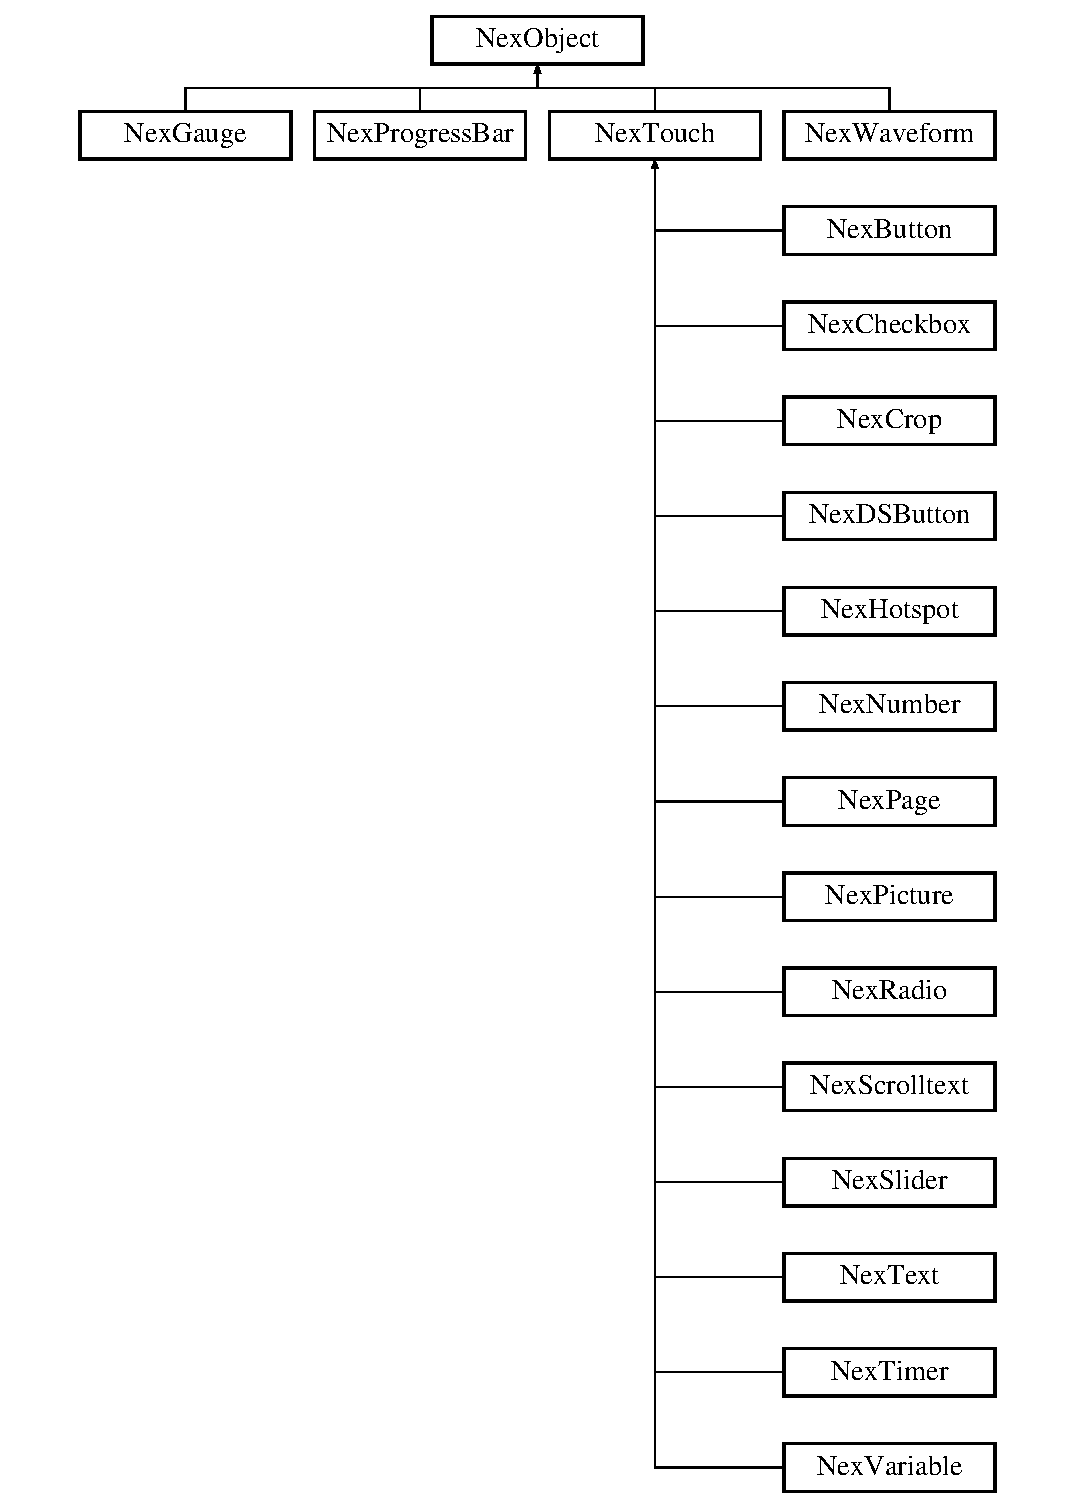
\includegraphics[height=12.000000cm]{class_nex_object}
\end{center}
\end{figure}
\subsection*{Public Member Functions}
\begin{DoxyCompactItemize}
\item 
\hyperlink{class_nex_object_ab15aadb9c91d9690786d8d25d12d94e1}{Nex\+Object} (uint8\+\_\+t pid, uint8\+\_\+t cid, const char $\ast$name)
\item 
void \hyperlink{class_nex_object_abeff0c61474e8b3ce6bac76771820b64}{print\+Obj\+Info} (void)
\end{DoxyCompactItemize}
\subsection*{Protected Member Functions}
\begin{DoxyCompactItemize}
\item 
\hypertarget{class_nex_object_a67621e5d7bcfb50c1a1bbc4ad1020352}{uint8\+\_\+t {\bfseries get\+Obj\+Pid} (void)}\label{class_nex_object_a67621e5d7bcfb50c1a1bbc4ad1020352}

\item 
\hypertarget{class_nex_object_a8139b294806c1684fc95b635a33b1b15}{uint8\+\_\+t {\bfseries get\+Obj\+Cid} (void)}\label{class_nex_object_a8139b294806c1684fc95b635a33b1b15}

\item 
\hypertarget{class_nex_object_aea0246c02cd5e54d0dbd714ace1ff2b1}{const char $\ast$ {\bfseries get\+Obj\+Name} (void)}\label{class_nex_object_aea0246c02cd5e54d0dbd714ace1ff2b1}

\end{DoxyCompactItemize}


\subsection{Detailed Description}
Root class of all Nextion components.

Provides the essential attributes of a Nextion component and the methods accessing them. At least, Page I\+D(pid), Component I\+D(pid) and an unique name are needed for creating a component in Nexiton library. 

\subsection{Constructor \& Destructor Documentation}
\hypertarget{class_nex_object_ab15aadb9c91d9690786d8d25d12d94e1}{\index{Nex\+Object@{Nex\+Object}!Nex\+Object@{Nex\+Object}}
\index{Nex\+Object@{Nex\+Object}!Nex\+Object@{Nex\+Object}}
\subsubsection[{Nex\+Object}]{\setlength{\rightskip}{0pt plus 5cm}Nex\+Object\+::\+Nex\+Object (
\begin{DoxyParamCaption}
\item[{uint8\+\_\+t}]{pid, }
\item[{uint8\+\_\+t}]{cid, }
\item[{const char $\ast$}]{name}
\end{DoxyParamCaption}
)}}\label{class_nex_object_ab15aadb9c91d9690786d8d25d12d94e1}
Constructor.


\begin{DoxyParams}{Parameters}
{\em pid} & -\/ page id. \\
\hline
{\em cid} & -\/ component id. \\
\hline
{\em name} & -\/ pointer to an unique name in range of all components. \\
\hline
\end{DoxyParams}


\subsection{Member Function Documentation}
\hypertarget{class_nex_object_abeff0c61474e8b3ce6bac76771820b64}{\index{Nex\+Object@{Nex\+Object}!print\+Obj\+Info@{print\+Obj\+Info}}
\index{print\+Obj\+Info@{print\+Obj\+Info}!Nex\+Object@{Nex\+Object}}
\subsubsection[{print\+Obj\+Info}]{\setlength{\rightskip}{0pt plus 5cm}void Nex\+Object\+::print\+Obj\+Info (
\begin{DoxyParamCaption}
\item[{void}]{}
\end{DoxyParamCaption}
)}}\label{class_nex_object_abeff0c61474e8b3ce6bac76771820b64}
Print current object'address, page id, component id and name.

\begin{DoxyWarning}{Warning}
this method does nothing, unless debug message enabled. 
\end{DoxyWarning}


The documentation for this class was generated from the following files\+:\begin{DoxyCompactItemize}
\item 
\hyperlink{_nex_object_8h}{Nex\+Object.\+h}\item 
\hyperlink{_nex_object_8cpp}{Nex\+Object.\+cpp}\end{DoxyCompactItemize}

\hypertarget{class_nex_page}{\section{Nex\+Page Class Reference}
\label{class_nex_page}\index{Nex\+Page@{Nex\+Page}}
}


{\ttfamily \#include $<$Nex\+Page.\+h$>$}

Inheritance diagram for Nex\+Page\+:\begin{figure}[H]
\begin{center}
\leavevmode
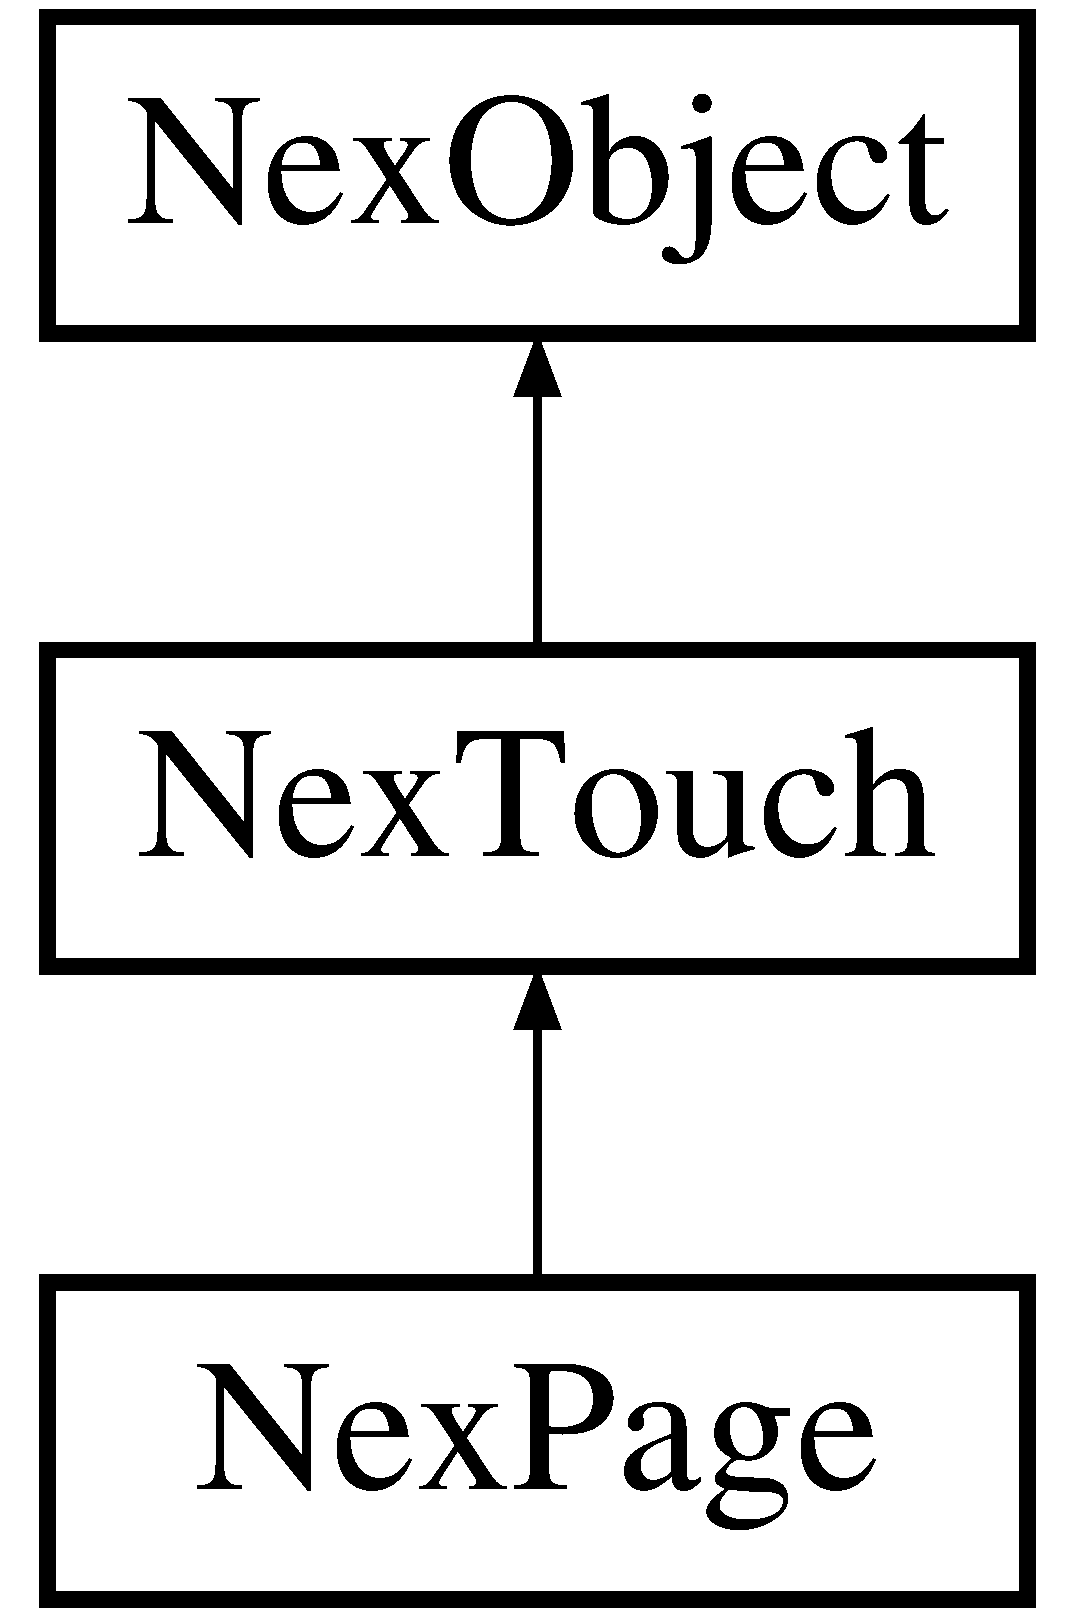
\includegraphics[height=3.000000cm]{class_nex_page}
\end{center}
\end{figure}
\subsection*{Public Member Functions}
\begin{DoxyCompactItemize}
\item 
\hyperlink{class_nex_page_a8608a0400bd8e27466ca4bbc05b5c2a0}{Nex\+Page} (uint8\+\_\+t pid, uint8\+\_\+t cid, const char $\ast$name)
\item 
bool \hyperlink{class_nex_page_a5714e41d4528b991eda4bbe578005418}{show} (void)
\end{DoxyCompactItemize}
\subsection*{Additional Inherited Members}


\subsection{Detailed Description}
A special component , which can contain other components such as \hyperlink{class_nex_button}{Nex\+Button}, \hyperlink{class_nex_text}{Nex\+Text} and \hyperlink{class_nex_waveform}{Nex\+Waveform}, etc. 

\subsection{Constructor \& Destructor Documentation}
\hypertarget{class_nex_page_a8608a0400bd8e27466ca4bbc05b5c2a0}{\index{Nex\+Page@{Nex\+Page}!Nex\+Page@{Nex\+Page}}
\index{Nex\+Page@{Nex\+Page}!Nex\+Page@{Nex\+Page}}
\subsubsection[{Nex\+Page}]{\setlength{\rightskip}{0pt plus 5cm}Nex\+Page\+::\+Nex\+Page (
\begin{DoxyParamCaption}
\item[{uint8\+\_\+t}]{pid, }
\item[{uint8\+\_\+t}]{cid, }
\item[{const char $\ast$}]{name}
\end{DoxyParamCaption}
)}}\label{class_nex_page_a8608a0400bd8e27466ca4bbc05b5c2a0}




Constructor.


\begin{DoxyParams}{Parameters}
{\em pid} & -\/ page id. \\
\hline
{\em cid} & -\/ component id. \\
\hline
{\em name} & -\/ pointer to an unique name in range of all components. \\
\hline
\end{DoxyParams}


\subsection{Member Function Documentation}
\hypertarget{class_nex_page_a5714e41d4528b991eda4bbe578005418}{\index{Nex\+Page@{Nex\+Page}!show@{show}}
\index{show@{show}!Nex\+Page@{Nex\+Page}}
\subsubsection[{show}]{\setlength{\rightskip}{0pt plus 5cm}bool Nex\+Page\+::show (
\begin{DoxyParamCaption}
\item[{void}]{}
\end{DoxyParamCaption}
)}}\label{class_nex_page_a5714e41d4528b991eda4bbe578005418}
Show itself.

\begin{DoxyReturn}{Returns}
true if success, false for faileure. 
\end{DoxyReturn}


The documentation for this class was generated from the following files\+:\begin{DoxyCompactItemize}
\item 
\hyperlink{_nex_page_8h}{Nex\+Page.\+h}\item 
\hyperlink{_nex_page_8cpp}{Nex\+Page.\+cpp}\end{DoxyCompactItemize}

\hypertarget{class_nex_picture}{\section{Nex\+Picture Class Reference}
\label{class_nex_picture}\index{Nex\+Picture@{Nex\+Picture}}
}


{\ttfamily \#include $<$Nex\+Picture.\+h$>$}

Inheritance diagram for Nex\+Picture\+:\begin{figure}[H]
\begin{center}
\leavevmode
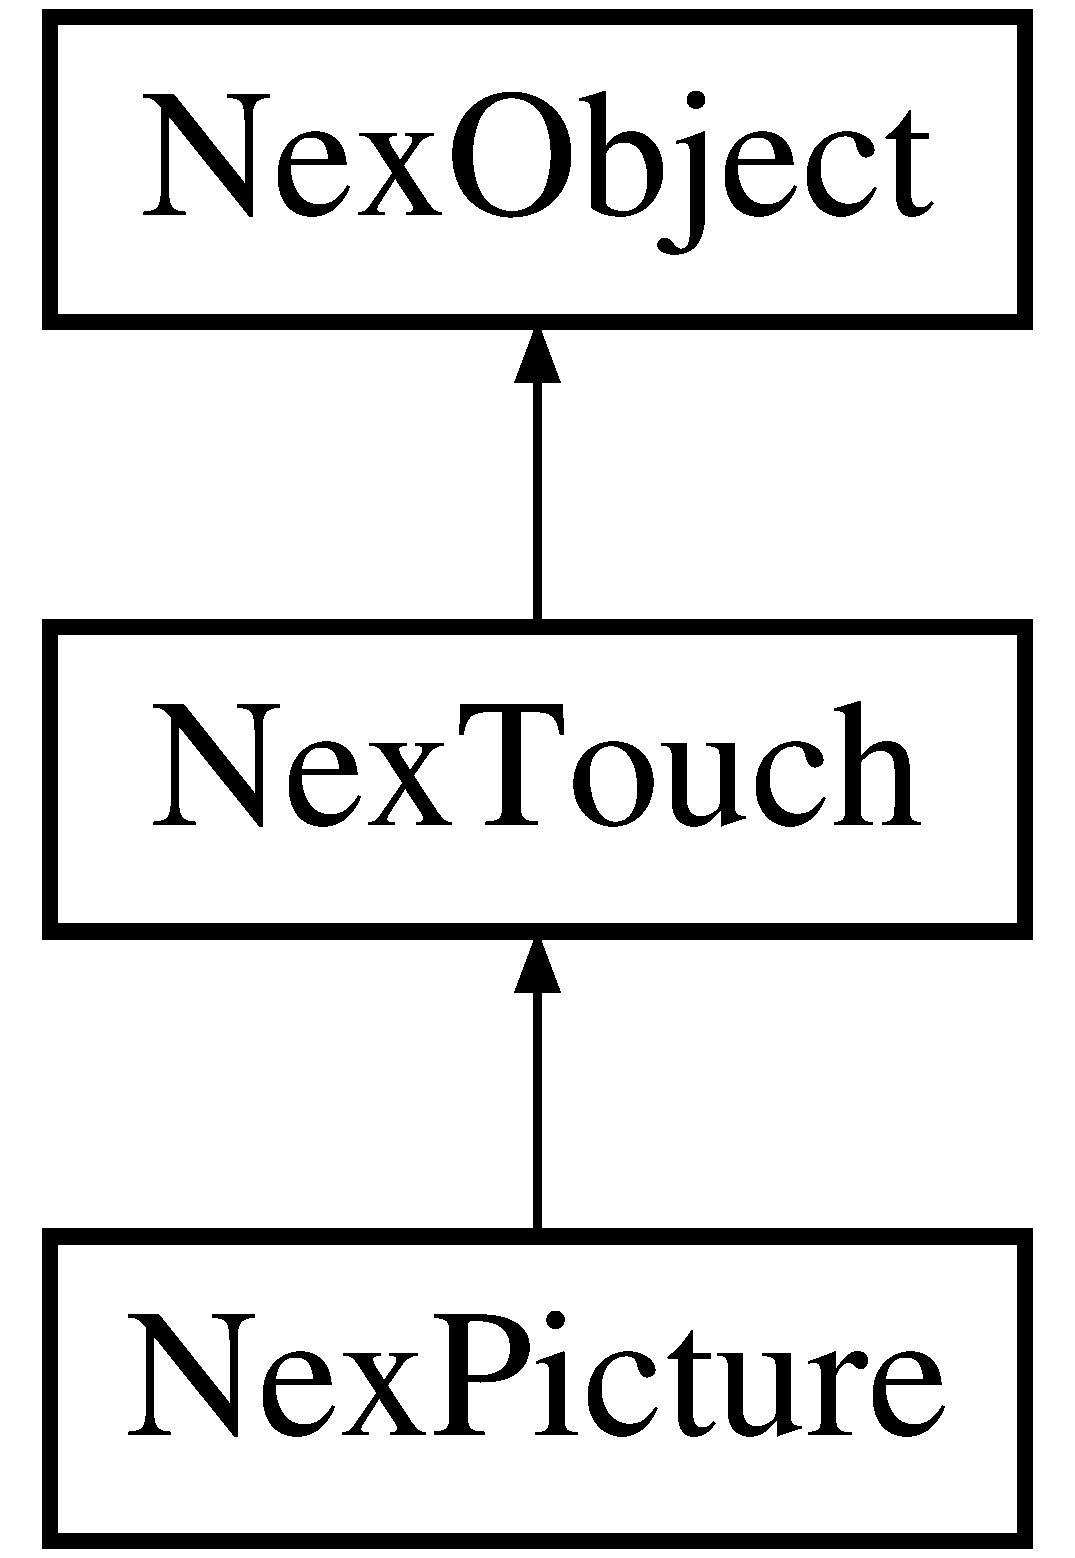
\includegraphics[height=3.000000cm]{class_nex_picture}
\end{center}
\end{figure}
\subsection*{Public Member Functions}
\begin{DoxyCompactItemize}
\item 
\hyperlink{class_nex_picture_aa6096defacd933e8bff5283c83200459}{Nex\+Picture} (uint8\+\_\+t pid, uint8\+\_\+t cid, const char $\ast$name)
\item 
bool \hyperlink{class_nex_picture_a0297c4a9544df9b0c37db0ea894d699f}{Get\+\_\+background\+\_\+image\+\_\+pic} (uint32\+\_\+t $\ast$number)
\item 
bool \hyperlink{class_nex_picture_a531e22f70dbf0dcaf6e114581364acea}{Set\+\_\+background\+\_\+image\+\_\+pic} (uint32\+\_\+t number)
\item 
bool \hyperlink{class_nex_picture_a11bd68ef9fe1d03d9e0d02ef1c7527e9}{get\+Pic} (uint32\+\_\+t $\ast$number)
\item 
bool \hyperlink{class_nex_picture_ab1c6adff615d48261ce10c2095859abd}{set\+Pic} (uint32\+\_\+t number)
\end{DoxyCompactItemize}
\subsection*{Additional Inherited Members}


\subsection{Detailed Description}
\hyperlink{class_nex_picture}{Nex\+Picture} component. 

\subsection{Constructor \& Destructor Documentation}
\hypertarget{class_nex_picture_aa6096defacd933e8bff5283c83200459}{\index{Nex\+Picture@{Nex\+Picture}!Nex\+Picture@{Nex\+Picture}}
\index{Nex\+Picture@{Nex\+Picture}!Nex\+Picture@{Nex\+Picture}}
\subsubsection[{Nex\+Picture}]{\setlength{\rightskip}{0pt plus 5cm}Nex\+Picture\+::\+Nex\+Picture (
\begin{DoxyParamCaption}
\item[{uint8\+\_\+t}]{pid, }
\item[{uint8\+\_\+t}]{cid, }
\item[{const char $\ast$}]{name}
\end{DoxyParamCaption}
)}}\label{class_nex_picture_aa6096defacd933e8bff5283c83200459}




Constructor.


\begin{DoxyParams}{Parameters}
{\em pid} & -\/ page id. \\
\hline
{\em cid} & -\/ component id. \\
\hline
{\em name} & -\/ pointer to an unique name in range of all components. \\
\hline
\end{DoxyParams}


\subsection{Member Function Documentation}
\hypertarget{class_nex_picture_a0297c4a9544df9b0c37db0ea894d699f}{\index{Nex\+Picture@{Nex\+Picture}!Get\+\_\+background\+\_\+image\+\_\+pic@{Get\+\_\+background\+\_\+image\+\_\+pic}}
\index{Get\+\_\+background\+\_\+image\+\_\+pic@{Get\+\_\+background\+\_\+image\+\_\+pic}!Nex\+Picture@{Nex\+Picture}}
\subsubsection[{Get\+\_\+background\+\_\+image\+\_\+pic}]{\setlength{\rightskip}{0pt plus 5cm}bool Nex\+Picture\+::\+Get\+\_\+background\+\_\+image\+\_\+pic (
\begin{DoxyParamCaption}
\item[{uint32\+\_\+t $\ast$}]{number}
\end{DoxyParamCaption}
)}}\label{class_nex_picture_a0297c4a9544df9b0c37db0ea894d699f}
Get picture's number.


\begin{DoxyParams}{Parameters}
{\em number} & -\/ an output parameter to save picture number.\\
\hline
\end{DoxyParams}

\begin{DoxyRetVals}{Return values}
{\em true} & -\/ success. \\
\hline
{\em false} & -\/ failed. \\
\hline
\end{DoxyRetVals}
\hypertarget{class_nex_picture_a11bd68ef9fe1d03d9e0d02ef1c7527e9}{\index{Nex\+Picture@{Nex\+Picture}!get\+Pic@{get\+Pic}}
\index{get\+Pic@{get\+Pic}!Nex\+Picture@{Nex\+Picture}}
\subsubsection[{get\+Pic}]{\setlength{\rightskip}{0pt plus 5cm}bool Nex\+Picture\+::get\+Pic (
\begin{DoxyParamCaption}
\item[{uint32\+\_\+t $\ast$}]{number}
\end{DoxyParamCaption}
)}}\label{class_nex_picture_a11bd68ef9fe1d03d9e0d02ef1c7527e9}
Get picture's number.


\begin{DoxyParams}{Parameters}
{\em number} & -\/ an output parameter to save picture number.\\
\hline
\end{DoxyParams}

\begin{DoxyRetVals}{Return values}
{\em true} & -\/ success. \\
\hline
{\em false} & -\/ failed. \\
\hline
\end{DoxyRetVals}
\hypertarget{class_nex_picture_a531e22f70dbf0dcaf6e114581364acea}{\index{Nex\+Picture@{Nex\+Picture}!Set\+\_\+background\+\_\+image\+\_\+pic@{Set\+\_\+background\+\_\+image\+\_\+pic}}
\index{Set\+\_\+background\+\_\+image\+\_\+pic@{Set\+\_\+background\+\_\+image\+\_\+pic}!Nex\+Picture@{Nex\+Picture}}
\subsubsection[{Set\+\_\+background\+\_\+image\+\_\+pic}]{\setlength{\rightskip}{0pt plus 5cm}bool Nex\+Picture\+::\+Set\+\_\+background\+\_\+image\+\_\+pic (
\begin{DoxyParamCaption}
\item[{uint32\+\_\+t}]{number}
\end{DoxyParamCaption}
)}}\label{class_nex_picture_a531e22f70dbf0dcaf6e114581364acea}
Set picture's number.


\begin{DoxyParams}{Parameters}
{\em number} & -\/the picture number.\\
\hline
\end{DoxyParams}

\begin{DoxyRetVals}{Return values}
{\em true} & -\/ success. \\
\hline
{\em false} & -\/ failed. \\
\hline
\end{DoxyRetVals}
\hypertarget{class_nex_picture_ab1c6adff615d48261ce10c2095859abd}{\index{Nex\+Picture@{Nex\+Picture}!set\+Pic@{set\+Pic}}
\index{set\+Pic@{set\+Pic}!Nex\+Picture@{Nex\+Picture}}
\subsubsection[{set\+Pic}]{\setlength{\rightskip}{0pt plus 5cm}bool Nex\+Picture\+::set\+Pic (
\begin{DoxyParamCaption}
\item[{uint32\+\_\+t}]{number}
\end{DoxyParamCaption}
)}}\label{class_nex_picture_ab1c6adff615d48261ce10c2095859abd}
Set picture's number.


\begin{DoxyParams}{Parameters}
{\em number} & -\/the picture number.\\
\hline
\end{DoxyParams}

\begin{DoxyRetVals}{Return values}
{\em true} & -\/ success. \\
\hline
{\em false} & -\/ failed. \\
\hline
\end{DoxyRetVals}


The documentation for this class was generated from the following files\+:\begin{DoxyCompactItemize}
\item 
\hyperlink{_nex_picture_8h}{Nex\+Picture.\+h}\item 
\hyperlink{_nex_picture_8cpp}{Nex\+Picture.\+cpp}\end{DoxyCompactItemize}

\hypertarget{class_nex_progress_bar}{\section{Nex\+Progress\+Bar Class Reference}
\label{class_nex_progress_bar}\index{Nex\+Progress\+Bar@{Nex\+Progress\+Bar}}
}


{\ttfamily \#include $<$Nex\+Progress\+Bar.\+h$>$}

Inheritance diagram for Nex\+Progress\+Bar\+:\begin{figure}[H]
\begin{center}
\leavevmode
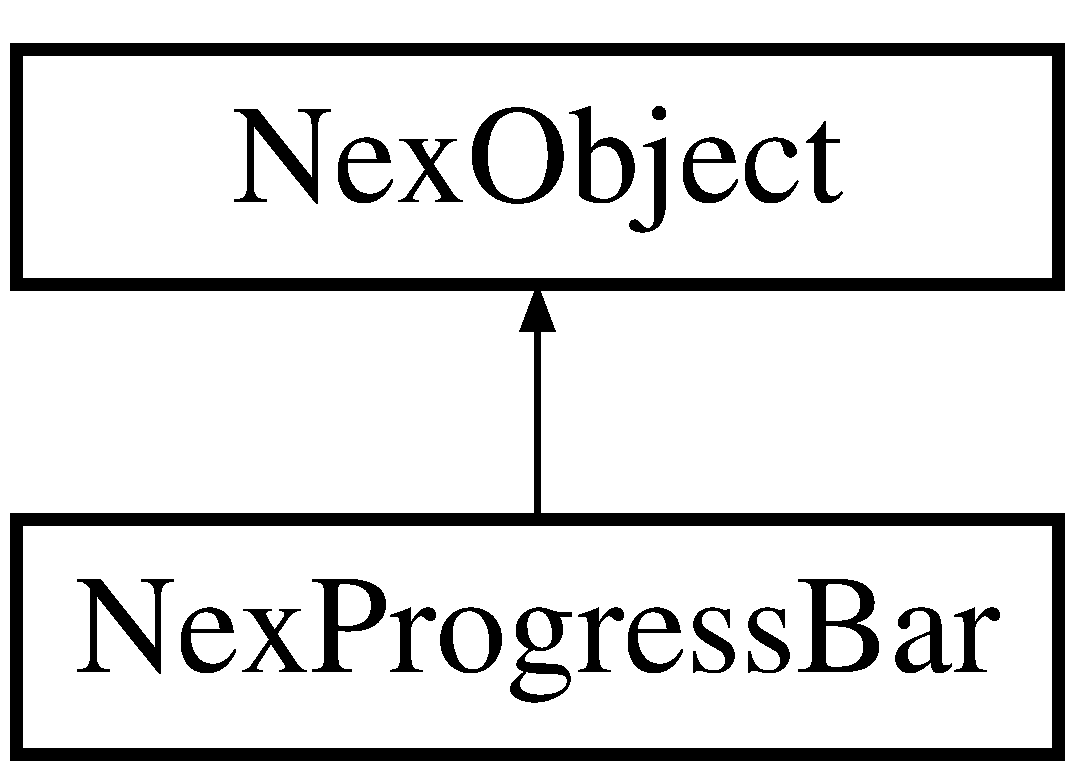
\includegraphics[height=2.000000cm]{class_nex_progress_bar}
\end{center}
\end{figure}
\subsection*{Public Member Functions}
\begin{DoxyCompactItemize}
\item 
\hyperlink{class_nex_progress_bar_a61f76f0c855c7839630dbc930e3401d8}{Nex\+Progress\+Bar} (uint8\+\_\+t pid, uint8\+\_\+t cid, const char $\ast$name)
\item 
bool \hyperlink{class_nex_progress_bar_a3e5eb13b2aa014c8f6a9e16439917bf2}{get\+Value} (uint32\+\_\+t $\ast$number)
\item 
bool \hyperlink{class_nex_progress_bar_aaa7937d364cb63151bd1e1bc4729334d}{set\+Value} (uint32\+\_\+t number)
\item 
uint32\+\_\+t \hyperlink{class_nex_progress_bar_a2efc0d6694d8739fb9caa31c53190271}{Get\+\_\+background\+\_\+color\+\_\+bco} (uint32\+\_\+t $\ast$number)
\item 
bool \hyperlink{class_nex_progress_bar_ab0b4230a6559989080e2a7b66b42ffc1}{Set\+\_\+background\+\_\+color\+\_\+bco} (uint32\+\_\+t number)
\item 
uint32\+\_\+t \hyperlink{class_nex_progress_bar_aa148721b86c5f56c6321780da3ef974f}{Get\+\_\+font\+\_\+color\+\_\+pco} (uint32\+\_\+t $\ast$number)
\item 
bool \hyperlink{class_nex_progress_bar_a0ee8478a28a3c31d4b7179317299f711}{Set\+\_\+font\+\_\+color\+\_\+pco} (uint32\+\_\+t number)
\end{DoxyCompactItemize}
\subsection*{Additional Inherited Members}


\subsection{Detailed Description}
\hyperlink{class_nex_progress_bar}{Nex\+Progress\+Bar} component. 

\subsection{Constructor \& Destructor Documentation}
\hypertarget{class_nex_progress_bar_a61f76f0c855c7839630dbc930e3401d8}{\index{Nex\+Progress\+Bar@{Nex\+Progress\+Bar}!Nex\+Progress\+Bar@{Nex\+Progress\+Bar}}
\index{Nex\+Progress\+Bar@{Nex\+Progress\+Bar}!Nex\+Progress\+Bar@{Nex\+Progress\+Bar}}
\subsubsection[{Nex\+Progress\+Bar}]{\setlength{\rightskip}{0pt plus 5cm}Nex\+Progress\+Bar\+::\+Nex\+Progress\+Bar (
\begin{DoxyParamCaption}
\item[{uint8\+\_\+t}]{pid, }
\item[{uint8\+\_\+t}]{cid, }
\item[{const char $\ast$}]{name}
\end{DoxyParamCaption}
)}}\label{class_nex_progress_bar_a61f76f0c855c7839630dbc930e3401d8}




Constructor.


\begin{DoxyParams}{Parameters}
{\em pid} & -\/ page id. \\
\hline
{\em cid} & -\/ component id. \\
\hline
{\em name} & -\/ pointer to an unique name in range of all components. \\
\hline
\end{DoxyParams}


\subsection{Member Function Documentation}
\hypertarget{class_nex_progress_bar_a2efc0d6694d8739fb9caa31c53190271}{\index{Nex\+Progress\+Bar@{Nex\+Progress\+Bar}!Get\+\_\+background\+\_\+color\+\_\+bco@{Get\+\_\+background\+\_\+color\+\_\+bco}}
\index{Get\+\_\+background\+\_\+color\+\_\+bco@{Get\+\_\+background\+\_\+color\+\_\+bco}!Nex\+Progress\+Bar@{Nex\+Progress\+Bar}}
\subsubsection[{Get\+\_\+background\+\_\+color\+\_\+bco}]{\setlength{\rightskip}{0pt plus 5cm}uint32\+\_\+t Nex\+Progress\+Bar\+::\+Get\+\_\+background\+\_\+color\+\_\+bco (
\begin{DoxyParamCaption}
\item[{uint32\+\_\+t $\ast$}]{number}
\end{DoxyParamCaption}
)}}\label{class_nex_progress_bar_a2efc0d6694d8739fb9caa31c53190271}
Get bco attribute of component


\begin{DoxyParams}{Parameters}
{\em number} & -\/ buffer storing data retur \\
\hline
\end{DoxyParams}
\begin{DoxyReturn}{Returns}
the length of the data 
\end{DoxyReturn}
\hypertarget{class_nex_progress_bar_aa148721b86c5f56c6321780da3ef974f}{\index{Nex\+Progress\+Bar@{Nex\+Progress\+Bar}!Get\+\_\+font\+\_\+color\+\_\+pco@{Get\+\_\+font\+\_\+color\+\_\+pco}}
\index{Get\+\_\+font\+\_\+color\+\_\+pco@{Get\+\_\+font\+\_\+color\+\_\+pco}!Nex\+Progress\+Bar@{Nex\+Progress\+Bar}}
\subsubsection[{Get\+\_\+font\+\_\+color\+\_\+pco}]{\setlength{\rightskip}{0pt plus 5cm}uint32\+\_\+t Nex\+Progress\+Bar\+::\+Get\+\_\+font\+\_\+color\+\_\+pco (
\begin{DoxyParamCaption}
\item[{uint32\+\_\+t $\ast$}]{number}
\end{DoxyParamCaption}
)}}\label{class_nex_progress_bar_aa148721b86c5f56c6321780da3ef974f}
Get pco attribute of component


\begin{DoxyParams}{Parameters}
{\em number} & -\/ buffer storing data retur \\
\hline
\end{DoxyParams}
\begin{DoxyReturn}{Returns}
the length of the data 
\end{DoxyReturn}
\hypertarget{class_nex_progress_bar_a3e5eb13b2aa014c8f6a9e16439917bf2}{\index{Nex\+Progress\+Bar@{Nex\+Progress\+Bar}!get\+Value@{get\+Value}}
\index{get\+Value@{get\+Value}!Nex\+Progress\+Bar@{Nex\+Progress\+Bar}}
\subsubsection[{get\+Value}]{\setlength{\rightskip}{0pt plus 5cm}bool Nex\+Progress\+Bar\+::get\+Value (
\begin{DoxyParamCaption}
\item[{uint32\+\_\+t $\ast$}]{number}
\end{DoxyParamCaption}
)}}\label{class_nex_progress_bar_a3e5eb13b2aa014c8f6a9e16439917bf2}
Get the value of progress bar.


\begin{DoxyParams}{Parameters}
{\em number} & -\/ an output parameter to save the value of porgress bar.\\
\hline
\end{DoxyParams}

\begin{DoxyRetVals}{Return values}
{\em true} & -\/ success. \\
\hline
{\em false} & -\/ failed. \\
\hline
\end{DoxyRetVals}
\hypertarget{class_nex_progress_bar_ab0b4230a6559989080e2a7b66b42ffc1}{\index{Nex\+Progress\+Bar@{Nex\+Progress\+Bar}!Set\+\_\+background\+\_\+color\+\_\+bco@{Set\+\_\+background\+\_\+color\+\_\+bco}}
\index{Set\+\_\+background\+\_\+color\+\_\+bco@{Set\+\_\+background\+\_\+color\+\_\+bco}!Nex\+Progress\+Bar@{Nex\+Progress\+Bar}}
\subsubsection[{Set\+\_\+background\+\_\+color\+\_\+bco}]{\setlength{\rightskip}{0pt plus 5cm}bool Nex\+Progress\+Bar\+::\+Set\+\_\+background\+\_\+color\+\_\+bco (
\begin{DoxyParamCaption}
\item[{uint32\+\_\+t}]{number}
\end{DoxyParamCaption}
)}}\label{class_nex_progress_bar_ab0b4230a6559989080e2a7b66b42ffc1}
Set bco attribute of component


\begin{DoxyParams}{Parameters}
{\em number} & -\/ To set up the data \\
\hline
\end{DoxyParams}
\begin{DoxyReturn}{Returns}
true if success, false for failure 
\end{DoxyReturn}
\hypertarget{class_nex_progress_bar_a0ee8478a28a3c31d4b7179317299f711}{\index{Nex\+Progress\+Bar@{Nex\+Progress\+Bar}!Set\+\_\+font\+\_\+color\+\_\+pco@{Set\+\_\+font\+\_\+color\+\_\+pco}}
\index{Set\+\_\+font\+\_\+color\+\_\+pco@{Set\+\_\+font\+\_\+color\+\_\+pco}!Nex\+Progress\+Bar@{Nex\+Progress\+Bar}}
\subsubsection[{Set\+\_\+font\+\_\+color\+\_\+pco}]{\setlength{\rightskip}{0pt plus 5cm}bool Nex\+Progress\+Bar\+::\+Set\+\_\+font\+\_\+color\+\_\+pco (
\begin{DoxyParamCaption}
\item[{uint32\+\_\+t}]{number}
\end{DoxyParamCaption}
)}}\label{class_nex_progress_bar_a0ee8478a28a3c31d4b7179317299f711}
Set pco attribute of component


\begin{DoxyParams}{Parameters}
{\em number} & -\/ To set up the data \\
\hline
\end{DoxyParams}
\begin{DoxyReturn}{Returns}
true if success, false for failure 
\end{DoxyReturn}
\hypertarget{class_nex_progress_bar_aaa7937d364cb63151bd1e1bc4729334d}{\index{Nex\+Progress\+Bar@{Nex\+Progress\+Bar}!set\+Value@{set\+Value}}
\index{set\+Value@{set\+Value}!Nex\+Progress\+Bar@{Nex\+Progress\+Bar}}
\subsubsection[{set\+Value}]{\setlength{\rightskip}{0pt plus 5cm}bool Nex\+Progress\+Bar\+::set\+Value (
\begin{DoxyParamCaption}
\item[{uint32\+\_\+t}]{number}
\end{DoxyParamCaption}
)}}\label{class_nex_progress_bar_aaa7937d364cb63151bd1e1bc4729334d}
Set the value of progress bar.


\begin{DoxyParams}{Parameters}
{\em number} & -\/ the value of progress bar.\\
\hline
\end{DoxyParams}

\begin{DoxyRetVals}{Return values}
{\em true} & -\/ success. \\
\hline
{\em false} & -\/ failed. \\
\hline
\end{DoxyRetVals}


The documentation for this class was generated from the following files\+:\begin{DoxyCompactItemize}
\item 
\hyperlink{_nex_progress_bar_8h}{Nex\+Progress\+Bar.\+h}\item 
\hyperlink{_nex_progress_bar_8cpp}{Nex\+Progress\+Bar.\+cpp}\end{DoxyCompactItemize}

\hypertarget{class_nex_radio}{\section{Nex\+Radio Class Reference}
\label{class_nex_radio}\index{Nex\+Radio@{Nex\+Radio}}
}


{\ttfamily \#include $<$Nex\+Radio.\+h$>$}

Inheritance diagram for Nex\+Radio\+:\begin{figure}[H]
\begin{center}
\leavevmode
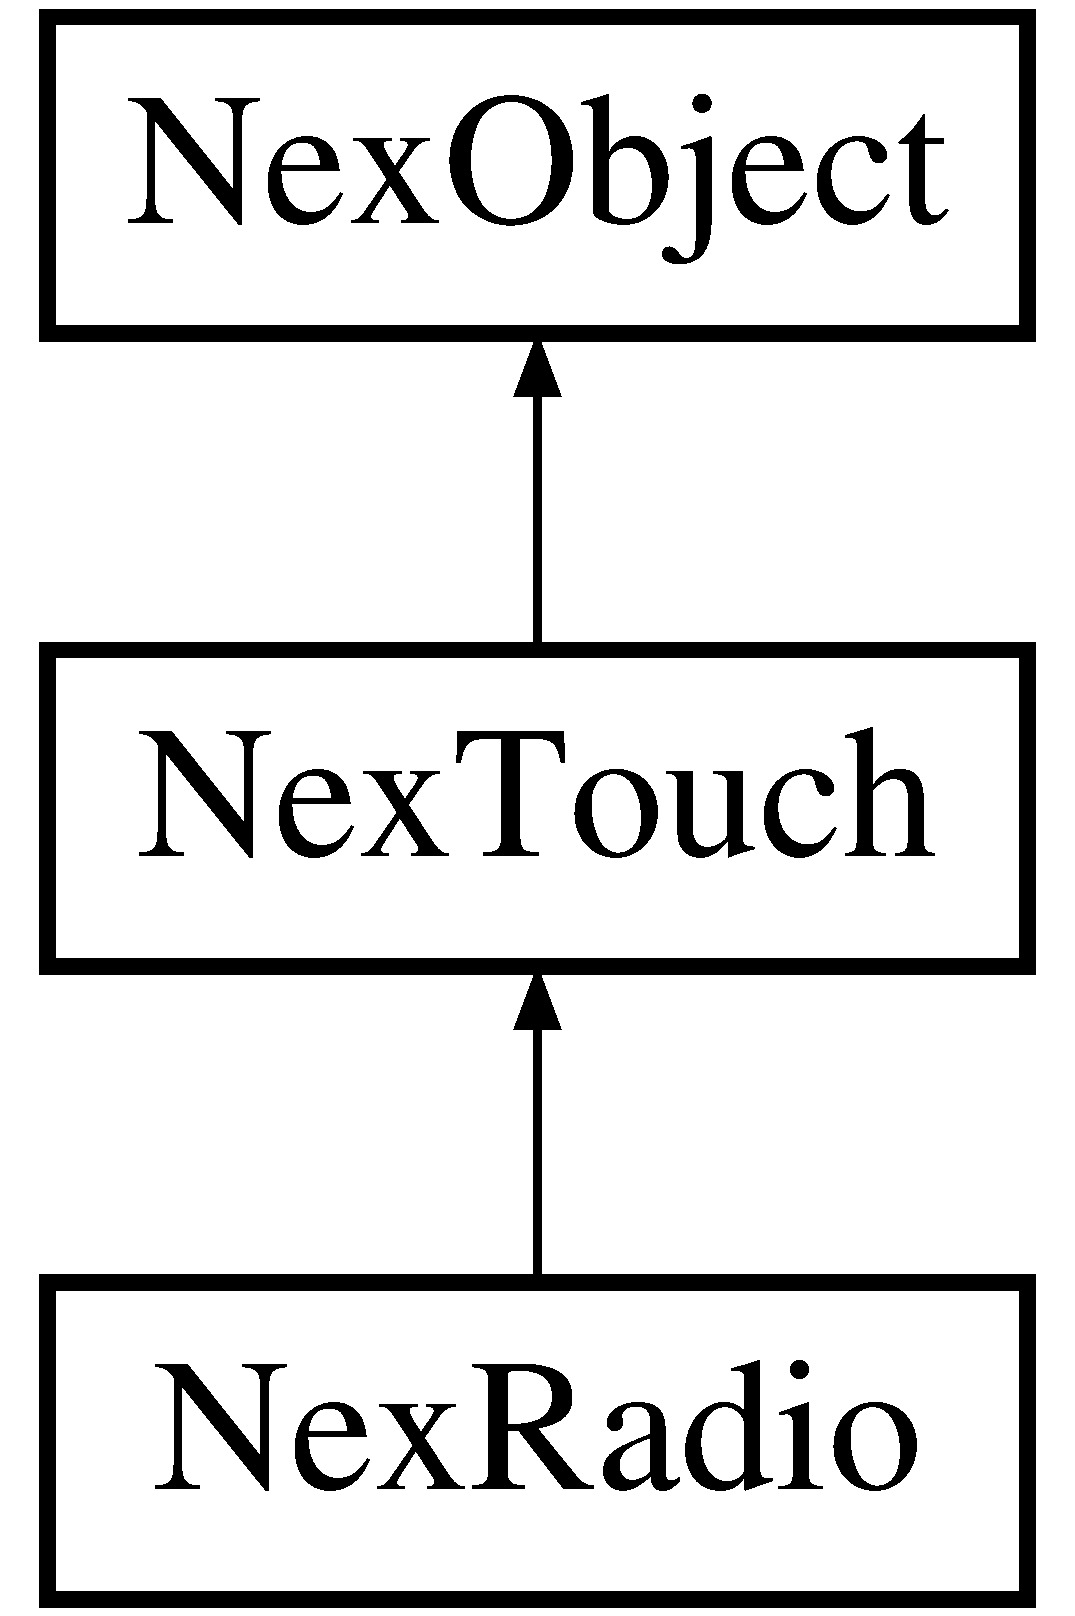
\includegraphics[height=3.000000cm]{class_nex_radio}
\end{center}
\end{figure}
\subsection*{Public Member Functions}
\begin{DoxyCompactItemize}
\item 
\hyperlink{class_nex_radio_a52264cd95aaa3ba7b4b07bdf64bb7a65}{Nex\+Radio} (uint8\+\_\+t pid, uint8\+\_\+t cid, const char $\ast$name)
\item 
uint32\+\_\+t \hyperlink{class_nex_radio_adb3672f10ce98ec7ad22f7b29a9ec0e6}{get\+Value} (uint32\+\_\+t $\ast$number)
\item 
bool \hyperlink{class_nex_radio_aa92d6f41ff30467a965e8a802e7d8b83}{set\+Value} (uint32\+\_\+t number)
\item 
uint32\+\_\+t \hyperlink{class_nex_radio_abdc8f654237d900eb3ddc955bc9e0038}{Get\+\_\+background\+\_\+color\+\_\+bco} (uint32\+\_\+t $\ast$number)
\item 
bool \hyperlink{class_nex_radio_a7bbd252dc78876d0831badbe791dbbc8}{Set\+\_\+background\+\_\+color\+\_\+bco} (uint32\+\_\+t number)
\item 
uint32\+\_\+t \hyperlink{class_nex_radio_a7a052fb745dfea5fe6f341692eb0ca1a}{Get\+\_\+font\+\_\+color\+\_\+pco} (uint32\+\_\+t $\ast$number)
\item 
bool \hyperlink{class_nex_radio_afd379837becbcf4a8f126820658a7f78}{Set\+\_\+font\+\_\+color\+\_\+pco} (uint32\+\_\+t number)
\end{DoxyCompactItemize}
\subsection*{Additional Inherited Members}


\subsection{Detailed Description}
\hyperlink{class_nex_radio}{Nex\+Radio} component.

Commonly, you want to do something after push and pop it. It is recommanded that only call \hyperlink{class_nex_touch_a4da1c4fcdfadb7eabfb9ccaba9ecad11}{Nex\+Touch\+::attach\+Pop} to satisfy your purpose.

\begin{DoxyWarning}{Warning}
Please do not call \hyperlink{class_nex_touch_a685a753aae5eb9fb9866a7807a310132}{Nex\+Touch\+::attach\+Push} on this component, even though you can. 
\end{DoxyWarning}


\subsection{Constructor \& Destructor Documentation}
\hypertarget{class_nex_radio_a52264cd95aaa3ba7b4b07bdf64bb7a65}{\index{Nex\+Radio@{Nex\+Radio}!Nex\+Radio@{Nex\+Radio}}
\index{Nex\+Radio@{Nex\+Radio}!Nex\+Radio@{Nex\+Radio}}
\subsubsection[{Nex\+Radio}]{\setlength{\rightskip}{0pt plus 5cm}Nex\+Radio\+::\+Nex\+Radio (
\begin{DoxyParamCaption}
\item[{uint8\+\_\+t}]{pid, }
\item[{uint8\+\_\+t}]{cid, }
\item[{const char $\ast$}]{name}
\end{DoxyParamCaption}
)}}\label{class_nex_radio_a52264cd95aaa3ba7b4b07bdf64bb7a65}




Constructor.


\begin{DoxyParams}{Parameters}
{\em pid} & -\/ page id. \\
\hline
{\em cid} & -\/ component id. \\
\hline
{\em name} & -\/ pointer to an unique name in range of all components. \\
\hline
\end{DoxyParams}


\subsection{Member Function Documentation}
\hypertarget{class_nex_radio_abdc8f654237d900eb3ddc955bc9e0038}{\index{Nex\+Radio@{Nex\+Radio}!Get\+\_\+background\+\_\+color\+\_\+bco@{Get\+\_\+background\+\_\+color\+\_\+bco}}
\index{Get\+\_\+background\+\_\+color\+\_\+bco@{Get\+\_\+background\+\_\+color\+\_\+bco}!Nex\+Radio@{Nex\+Radio}}
\subsubsection[{Get\+\_\+background\+\_\+color\+\_\+bco}]{\setlength{\rightskip}{0pt plus 5cm}uint32\+\_\+t Nex\+Radio\+::\+Get\+\_\+background\+\_\+color\+\_\+bco (
\begin{DoxyParamCaption}
\item[{uint32\+\_\+t $\ast$}]{number}
\end{DoxyParamCaption}
)}}\label{class_nex_radio_abdc8f654237d900eb3ddc955bc9e0038}
Get bco attribute of component


\begin{DoxyParams}{Parameters}
{\em number} & -\/ buffer storing data retur \\
\hline
\end{DoxyParams}
\begin{DoxyReturn}{Returns}
the length of the data 
\end{DoxyReturn}
\hypertarget{class_nex_radio_a7a052fb745dfea5fe6f341692eb0ca1a}{\index{Nex\+Radio@{Nex\+Radio}!Get\+\_\+font\+\_\+color\+\_\+pco@{Get\+\_\+font\+\_\+color\+\_\+pco}}
\index{Get\+\_\+font\+\_\+color\+\_\+pco@{Get\+\_\+font\+\_\+color\+\_\+pco}!Nex\+Radio@{Nex\+Radio}}
\subsubsection[{Get\+\_\+font\+\_\+color\+\_\+pco}]{\setlength{\rightskip}{0pt plus 5cm}uint32\+\_\+t Nex\+Radio\+::\+Get\+\_\+font\+\_\+color\+\_\+pco (
\begin{DoxyParamCaption}
\item[{uint32\+\_\+t $\ast$}]{number}
\end{DoxyParamCaption}
)}}\label{class_nex_radio_a7a052fb745dfea5fe6f341692eb0ca1a}
Get pco attribute of component


\begin{DoxyParams}{Parameters}
{\em number} & -\/ buffer storing data retur \\
\hline
\end{DoxyParams}
\begin{DoxyReturn}{Returns}
the length of the data 
\end{DoxyReturn}
\hypertarget{class_nex_radio_adb3672f10ce98ec7ad22f7b29a9ec0e6}{\index{Nex\+Radio@{Nex\+Radio}!get\+Value@{get\+Value}}
\index{get\+Value@{get\+Value}!Nex\+Radio@{Nex\+Radio}}
\subsubsection[{get\+Value}]{\setlength{\rightskip}{0pt plus 5cm}uint32\+\_\+t Nex\+Radio\+::get\+Value (
\begin{DoxyParamCaption}
\item[{uint32\+\_\+t $\ast$}]{number}
\end{DoxyParamCaption}
)}}\label{class_nex_radio_adb3672f10ce98ec7ad22f7b29a9ec0e6}
Get val attribute of component


\begin{DoxyParams}{Parameters}
{\em number} & -\/ buffer storing data retur \\
\hline
\end{DoxyParams}
\begin{DoxyReturn}{Returns}
the length of the data 
\end{DoxyReturn}
\hypertarget{class_nex_radio_a7bbd252dc78876d0831badbe791dbbc8}{\index{Nex\+Radio@{Nex\+Radio}!Set\+\_\+background\+\_\+color\+\_\+bco@{Set\+\_\+background\+\_\+color\+\_\+bco}}
\index{Set\+\_\+background\+\_\+color\+\_\+bco@{Set\+\_\+background\+\_\+color\+\_\+bco}!Nex\+Radio@{Nex\+Radio}}
\subsubsection[{Set\+\_\+background\+\_\+color\+\_\+bco}]{\setlength{\rightskip}{0pt plus 5cm}bool Nex\+Radio\+::\+Set\+\_\+background\+\_\+color\+\_\+bco (
\begin{DoxyParamCaption}
\item[{uint32\+\_\+t}]{number}
\end{DoxyParamCaption}
)}}\label{class_nex_radio_a7bbd252dc78876d0831badbe791dbbc8}
Set bco attribute of component


\begin{DoxyParams}{Parameters}
{\em number} & -\/ To set up the data \\
\hline
\end{DoxyParams}
\begin{DoxyReturn}{Returns}
true if success, false for failure 
\end{DoxyReturn}
\hypertarget{class_nex_radio_afd379837becbcf4a8f126820658a7f78}{\index{Nex\+Radio@{Nex\+Radio}!Set\+\_\+font\+\_\+color\+\_\+pco@{Set\+\_\+font\+\_\+color\+\_\+pco}}
\index{Set\+\_\+font\+\_\+color\+\_\+pco@{Set\+\_\+font\+\_\+color\+\_\+pco}!Nex\+Radio@{Nex\+Radio}}
\subsubsection[{Set\+\_\+font\+\_\+color\+\_\+pco}]{\setlength{\rightskip}{0pt plus 5cm}bool Nex\+Radio\+::\+Set\+\_\+font\+\_\+color\+\_\+pco (
\begin{DoxyParamCaption}
\item[{uint32\+\_\+t}]{number}
\end{DoxyParamCaption}
)}}\label{class_nex_radio_afd379837becbcf4a8f126820658a7f78}
Set pco attribute of component


\begin{DoxyParams}{Parameters}
{\em number} & -\/ To set up the data \\
\hline
\end{DoxyParams}
\begin{DoxyReturn}{Returns}
true if success, false for failure 
\end{DoxyReturn}
\hypertarget{class_nex_radio_aa92d6f41ff30467a965e8a802e7d8b83}{\index{Nex\+Radio@{Nex\+Radio}!set\+Value@{set\+Value}}
\index{set\+Value@{set\+Value}!Nex\+Radio@{Nex\+Radio}}
\subsubsection[{set\+Value}]{\setlength{\rightskip}{0pt plus 5cm}bool Nex\+Radio\+::set\+Value (
\begin{DoxyParamCaption}
\item[{uint32\+\_\+t}]{number}
\end{DoxyParamCaption}
)}}\label{class_nex_radio_aa92d6f41ff30467a965e8a802e7d8b83}
Set val attribute of component


\begin{DoxyParams}{Parameters}
{\em number} & -\/ To set up the data \\
\hline
\end{DoxyParams}
\begin{DoxyReturn}{Returns}
true if success, false for failure 
\end{DoxyReturn}


The documentation for this class was generated from the following files\+:\begin{DoxyCompactItemize}
\item 
\hyperlink{_nex_radio_8h}{Nex\+Radio.\+h}\item 
\hyperlink{_nex_radio_8cpp}{Nex\+Radio.\+cpp}\end{DoxyCompactItemize}

\hypertarget{class_nex_rtc}{\section{Nex\+Rtc Class Reference}
\label{class_nex_rtc}\index{Nex\+Rtc@{Nex\+Rtc}}
}
\subsection*{Public Member Functions}
\begin{DoxyCompactItemize}
\item 
\hypertarget{class_nex_rtc_acd9e74c0098ef55877b5ae070572dae4}{bool {\bfseries write\+\_\+rtc\+\_\+time} (char $\ast$time)}\label{class_nex_rtc_acd9e74c0098ef55877b5ae070572dae4}

\item 
bool \hyperlink{class_nex_rtc_a9c55a15fa0a2b1511162facdc47f78b2}{write\+\_\+rtc\+\_\+time} (char $\ast$time\+\_\+type, uint32\+\_\+t number)
\item 
bool \hyperlink{class_nex_rtc_ab11da59341b52b0f686cb85a058d0962}{write\+\_\+rtc\+\_\+time} (uint32\+\_\+t $\ast$time)
\item 
uint32\+\_\+t \hyperlink{class_nex_rtc_a17230cd9342a905778fa4ee2e8609f02}{read\+\_\+rtc\+\_\+time} (char $\ast$time, uint32\+\_\+t len)
\item 
uint32\+\_\+t \hyperlink{class_nex_rtc_aa1afa1d516db55dfbbf650cbe5180eab}{read\+\_\+rtc\+\_\+time} (char $\ast$time\+\_\+type, uint32\+\_\+t $\ast$number)
\item 
uint32\+\_\+t \hyperlink{class_nex_rtc_ac71de2cd6f7598f05a5115642714d490}{read\+\_\+rtc\+\_\+time} (uint32\+\_\+t $\ast$time, uint32\+\_\+t len)
\end{DoxyCompactItemize}


\subsection{Member Function Documentation}
\hypertarget{class_nex_rtc_a17230cd9342a905778fa4ee2e8609f02}{\index{Nex\+Rtc@{Nex\+Rtc}!read\+\_\+rtc\+\_\+time@{read\+\_\+rtc\+\_\+time}}
\index{read\+\_\+rtc\+\_\+time@{read\+\_\+rtc\+\_\+time}!Nex\+Rtc@{Nex\+Rtc}}
\subsubsection[{read\+\_\+rtc\+\_\+time}]{\setlength{\rightskip}{0pt plus 5cm}uint32\+\_\+t Nex\+Rtc\+::read\+\_\+rtc\+\_\+time (
\begin{DoxyParamCaption}
\item[{char $\ast$}]{time, }
\item[{uint32\+\_\+t}]{len}
\end{DoxyParamCaption}
)}}\label{class_nex_rtc_a17230cd9342a905778fa4ee2e8609f02}
read rtc time


\begin{DoxyParams}{Parameters}
{\em time} & -\/ Access data array \\
\hline
{\em time} & -\/ len of array \\
\hline
\end{DoxyParams}
\begin{DoxyReturn}{Returns}
true if success, false for failure 
\end{DoxyReturn}
\hypertarget{class_nex_rtc_aa1afa1d516db55dfbbf650cbe5180eab}{\index{Nex\+Rtc@{Nex\+Rtc}!read\+\_\+rtc\+\_\+time@{read\+\_\+rtc\+\_\+time}}
\index{read\+\_\+rtc\+\_\+time@{read\+\_\+rtc\+\_\+time}!Nex\+Rtc@{Nex\+Rtc}}
\subsubsection[{read\+\_\+rtc\+\_\+time}]{\setlength{\rightskip}{0pt plus 5cm}uint32\+\_\+t Nex\+Rtc\+::read\+\_\+rtc\+\_\+time (
\begin{DoxyParamCaption}
\item[{char $\ast$}]{time\+\_\+type, }
\item[{uint32\+\_\+t $\ast$}]{number}
\end{DoxyParamCaption}
)}}\label{class_nex_rtc_aa1afa1d516db55dfbbf650cbe5180eab}
read rtc times


\begin{DoxyParams}{Parameters}
{\em time\+\_\+type} & -\/ To type in time \\
\hline
{\em number} & -\/ the time value \\
\hline
\end{DoxyParams}
\begin{DoxyReturn}{Returns}
true if success, false for failure 
\end{DoxyReturn}
\hypertarget{class_nex_rtc_ac71de2cd6f7598f05a5115642714d490}{\index{Nex\+Rtc@{Nex\+Rtc}!read\+\_\+rtc\+\_\+time@{read\+\_\+rtc\+\_\+time}}
\index{read\+\_\+rtc\+\_\+time@{read\+\_\+rtc\+\_\+time}!Nex\+Rtc@{Nex\+Rtc}}
\subsubsection[{read\+\_\+rtc\+\_\+time}]{\setlength{\rightskip}{0pt plus 5cm}uint32\+\_\+t Nex\+Rtc\+::read\+\_\+rtc\+\_\+time (
\begin{DoxyParamCaption}
\item[{uint32\+\_\+t $\ast$}]{time, }
\item[{uint32\+\_\+t}]{len}
\end{DoxyParamCaption}
)}}\label{class_nex_rtc_ac71de2cd6f7598f05a5115642714d490}
read rtc time


\begin{DoxyParams}{Parameters}
{\em time} & -\/ Access data array \\
\hline
{\em time} & -\/ len of array \\
\hline
\end{DoxyParams}
\begin{DoxyReturn}{Returns}
true if success, false for failure 
\end{DoxyReturn}
\hypertarget{class_nex_rtc_a9c55a15fa0a2b1511162facdc47f78b2}{\index{Nex\+Rtc@{Nex\+Rtc}!write\+\_\+rtc\+\_\+time@{write\+\_\+rtc\+\_\+time}}
\index{write\+\_\+rtc\+\_\+time@{write\+\_\+rtc\+\_\+time}!Nex\+Rtc@{Nex\+Rtc}}
\subsubsection[{write\+\_\+rtc\+\_\+time}]{\setlength{\rightskip}{0pt plus 5cm}bool Nex\+Rtc\+::write\+\_\+rtc\+\_\+time (
\begin{DoxyParamCaption}
\item[{char $\ast$}]{time\+\_\+type, }
\item[{uint32\+\_\+t}]{number}
\end{DoxyParamCaption}
)}}\label{class_nex_rtc_a9c55a15fa0a2b1511162facdc47f78b2}
write rtc times


\begin{DoxyParams}{Parameters}
{\em time\+\_\+type} & -\/ To type in time (example\+:write\+\_\+rtc\+\_\+time(\char`\"{}year\char`\"{},2016)) \\
\hline
{\em number} & -\/ the time value \\
\hline
\end{DoxyParams}
\begin{DoxyReturn}{Returns}
true if success, false for failure 
\end{DoxyReturn}
\hypertarget{class_nex_rtc_ab11da59341b52b0f686cb85a058d0962}{\index{Nex\+Rtc@{Nex\+Rtc}!write\+\_\+rtc\+\_\+time@{write\+\_\+rtc\+\_\+time}}
\index{write\+\_\+rtc\+\_\+time@{write\+\_\+rtc\+\_\+time}!Nex\+Rtc@{Nex\+Rtc}}
\subsubsection[{write\+\_\+rtc\+\_\+time}]{\setlength{\rightskip}{0pt plus 5cm}bool Nex\+Rtc\+::write\+\_\+rtc\+\_\+time (
\begin{DoxyParamCaption}
\item[{uint32\+\_\+t $\ast$}]{time}
\end{DoxyParamCaption}
)}}\label{class_nex_rtc_ab11da59341b52b0f686cb85a058d0962}
write rtc times


\begin{DoxyParams}{Parameters}
{\em time} & -\/ Time to write to the array \\
\hline
\end{DoxyParams}
\begin{DoxyReturn}{Returns}
true if success, false for failure 
\end{DoxyReturn}


The documentation for this class was generated from the following files\+:\begin{DoxyCompactItemize}
\item 
Nex\+Rtc.\+h\item 
\hyperlink{_nex_rtc_8cpp}{Nex\+Rtc.\+cpp}\end{DoxyCompactItemize}

\hypertarget{class_nex_scrolltext}{\section{Nex\+Scrolltext Class Reference}
\label{class_nex_scrolltext}\index{Nex\+Scrolltext@{Nex\+Scrolltext}}
}


{\ttfamily \#include $<$Nex\+Scrolltext.\+h$>$}

Inheritance diagram for Nex\+Scrolltext\+:\begin{figure}[H]
\begin{center}
\leavevmode
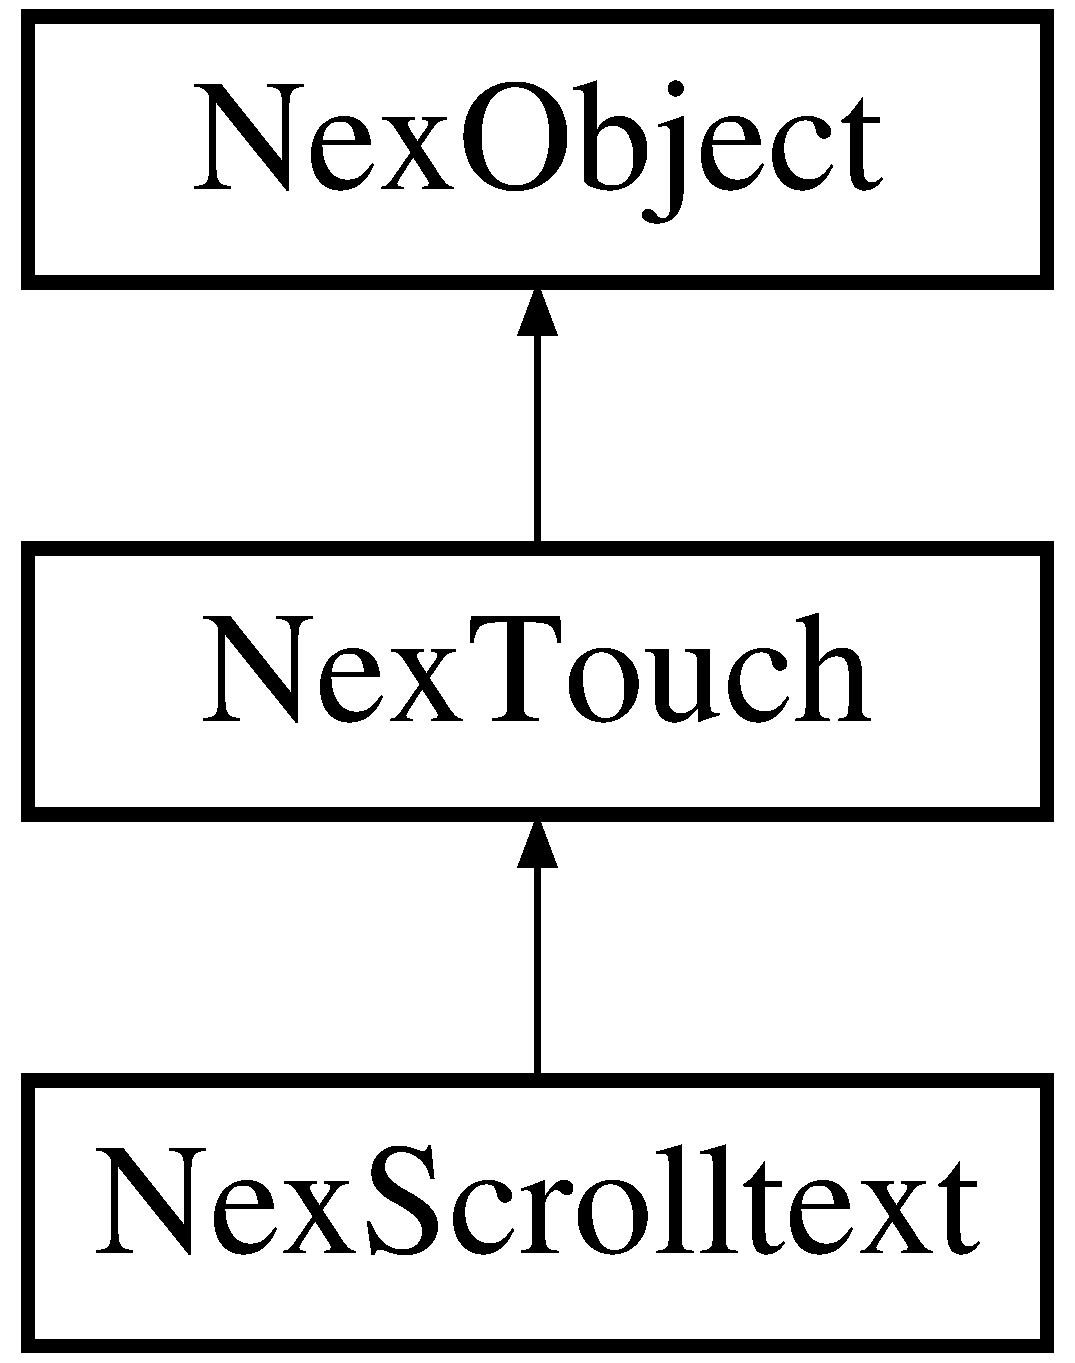
\includegraphics[height=3.000000cm]{class_nex_scrolltext}
\end{center}
\end{figure}
\subsection*{Public Member Functions}
\begin{DoxyCompactItemize}
\item 
\hyperlink{class_nex_scrolltext_a212aa1505ed7c0bfdb47de3e6e2045fb}{Nex\+Scrolltext} (uint8\+\_\+t pid, uint8\+\_\+t cid, const char $\ast$name)
\item 
uint16\+\_\+t \hyperlink{class_nex_scrolltext_a7cead053146075e7c31d43349d4c897c}{get\+Text} (char $\ast$buffer, uint16\+\_\+t len)
\item 
bool \hyperlink{class_nex_scrolltext_a71b8e2b2bff22e3c0cbdf961a55b8d12}{set\+Text} (const char $\ast$buffer)
\item 
uint32\+\_\+t \hyperlink{class_nex_scrolltext_ac3861fec5efd8cde4535307f231244e7}{Get\+\_\+background\+\_\+color\+\_\+bco} (uint32\+\_\+t $\ast$number)
\item 
bool \hyperlink{class_nex_scrolltext_a50a5211fc6913b97afda045a762cb0c4}{Set\+\_\+background\+\_\+color\+\_\+bco} (uint32\+\_\+t number)
\item 
uint32\+\_\+t \hyperlink{class_nex_scrolltext_a266a3c44131eec0a40b1e12f6cf7d3a1}{Get\+\_\+font\+\_\+color\+\_\+pco} (uint32\+\_\+t $\ast$number)
\item 
bool \hyperlink{class_nex_scrolltext_ac34d68211c4c3c70834c7e7e49ece03f}{Set\+\_\+font\+\_\+color\+\_\+pco} (uint32\+\_\+t number)
\item 
uint32\+\_\+t \hyperlink{class_nex_scrolltext_a066d8439ea088a7ef604abb87802add6}{Get\+\_\+place\+\_\+xcen} (uint32\+\_\+t $\ast$number)
\item 
bool \hyperlink{class_nex_scrolltext_a5126fc70854f0f12f1573ee1eb8959b0}{Set\+\_\+place\+\_\+xcen} (uint32\+\_\+t number)
\item 
uint32\+\_\+t \hyperlink{class_nex_scrolltext_a987a74978f764f74540c8ee0de200564}{Get\+\_\+place\+\_\+ycen} (uint32\+\_\+t $\ast$number)
\item 
bool \hyperlink{class_nex_scrolltext_ae1c1181755c9334a4ea21fa2782aecbf}{Set\+\_\+place\+\_\+ycen} (uint32\+\_\+t number)
\item 
uint32\+\_\+t \hyperlink{class_nex_scrolltext_a2caedb7b97a6028abedaf0b25f9c03e0}{get\+Font} (uint32\+\_\+t $\ast$number)
\item 
bool \hyperlink{class_nex_scrolltext_af2e8602fae103ccadfee037382844ce6}{set\+Font} (uint32\+\_\+t number)
\item 
uint32\+\_\+t \hyperlink{class_nex_scrolltext_a0d8e8997419f4d6460cc1e64f20cfb8c}{Get\+\_\+background\+\_\+crop\+\_\+picc} (uint32\+\_\+t $\ast$number)
\item 
bool \hyperlink{class_nex_scrolltext_a0a4d02fef0a0a1f9a1e41c66709b97c1}{Set\+\_\+background\+\_\+crop\+\_\+picc} (uint32\+\_\+t number)
\item 
uint32\+\_\+t \hyperlink{class_nex_scrolltext_a86ffab21e76beed5d801c05b94da6150}{Get\+\_\+background\+\_\+image\+\_\+pic} (uint32\+\_\+t $\ast$number)
\item 
bool \hyperlink{class_nex_scrolltext_a629fa1d39761144ec1e421c3c79a51aa}{Set\+\_\+background\+\_\+image\+\_\+pic} (uint32\+\_\+t number)
\item 
uint32\+\_\+t \hyperlink{class_nex_scrolltext_a4a437ad158a3be51e61dd469b77ee450}{Get\+\_\+scroll\+\_\+dir} (uint32\+\_\+t $\ast$number)
\item 
bool \hyperlink{class_nex_scrolltext_ad9ab4f129779d40fe5d108cac8c3a842}{Set\+\_\+scroll\+\_\+dir} (uint32\+\_\+t number)
\item 
uint32\+\_\+t \hyperlink{class_nex_scrolltext_a46ac65d7561b32fd4c5ac2f0aacf9bf1}{Get\+\_\+scroll\+\_\+distance} (uint32\+\_\+t $\ast$number)
\item 
bool \hyperlink{class_nex_scrolltext_a039a5f4dae5046142c4605097593545c}{Set\+\_\+scroll\+\_\+distance} (uint32\+\_\+t number)
\item 
uint32\+\_\+t \hyperlink{class_nex_scrolltext_a5d881dcad2360b42327cf95f8e91955f}{Get\+\_\+cycle\+\_\+tim} (uint32\+\_\+t $\ast$number)
\item 
bool \hyperlink{class_nex_scrolltext_ad639bf79aa963966241db4f45c7c8bd6}{Set\+\_\+cycle\+\_\+tim} (uint32\+\_\+t number)
\item 
\hypertarget{class_nex_scrolltext_a6941c1a200d0e4f913c5b37a7114b33a}{bool {\bfseries enable} (void)}\label{class_nex_scrolltext_a6941c1a200d0e4f913c5b37a7114b33a}

\item 
\hypertarget{class_nex_scrolltext_a909b5ec3d9b01a29715bf616dfafaeee}{bool {\bfseries disable} (void)}\label{class_nex_scrolltext_a909b5ec3d9b01a29715bf616dfafaeee}

\end{DoxyCompactItemize}
\subsection*{Additional Inherited Members}


\subsection{Detailed Description}
\hyperlink{class_nex_text}{Nex\+Text} component. 

\subsection{Constructor \& Destructor Documentation}
\hypertarget{class_nex_scrolltext_a212aa1505ed7c0bfdb47de3e6e2045fb}{\index{Nex\+Scrolltext@{Nex\+Scrolltext}!Nex\+Scrolltext@{Nex\+Scrolltext}}
\index{Nex\+Scrolltext@{Nex\+Scrolltext}!Nex\+Scrolltext@{Nex\+Scrolltext}}
\subsubsection[{Nex\+Scrolltext}]{\setlength{\rightskip}{0pt plus 5cm}Nex\+Scrolltext\+::\+Nex\+Scrolltext (
\begin{DoxyParamCaption}
\item[{uint8\+\_\+t}]{pid, }
\item[{uint8\+\_\+t}]{cid, }
\item[{const char $\ast$}]{name}
\end{DoxyParamCaption}
)}}\label{class_nex_scrolltext_a212aa1505ed7c0bfdb47de3e6e2045fb}




Constructor.


\begin{DoxyParams}{Parameters}
{\em pid} & -\/ page id. \\
\hline
{\em cid} & -\/ component id. \\
\hline
{\em name} & -\/ pointer to an unique name in range of all components. \\
\hline
\end{DoxyParams}


\subsection{Member Function Documentation}
\hypertarget{class_nex_scrolltext_ac3861fec5efd8cde4535307f231244e7}{\index{Nex\+Scrolltext@{Nex\+Scrolltext}!Get\+\_\+background\+\_\+color\+\_\+bco@{Get\+\_\+background\+\_\+color\+\_\+bco}}
\index{Get\+\_\+background\+\_\+color\+\_\+bco@{Get\+\_\+background\+\_\+color\+\_\+bco}!Nex\+Scrolltext@{Nex\+Scrolltext}}
\subsubsection[{Get\+\_\+background\+\_\+color\+\_\+bco}]{\setlength{\rightskip}{0pt plus 5cm}uint32\+\_\+t Nex\+Scrolltext\+::\+Get\+\_\+background\+\_\+color\+\_\+bco (
\begin{DoxyParamCaption}
\item[{uint32\+\_\+t $\ast$}]{number}
\end{DoxyParamCaption}
)}}\label{class_nex_scrolltext_ac3861fec5efd8cde4535307f231244e7}
Get bco attribute of component


\begin{DoxyParams}{Parameters}
{\em number} & -\/ buffer storing data retur \\
\hline
\end{DoxyParams}
\begin{DoxyReturn}{Returns}
the length of the data 
\end{DoxyReturn}
\hypertarget{class_nex_scrolltext_a0d8e8997419f4d6460cc1e64f20cfb8c}{\index{Nex\+Scrolltext@{Nex\+Scrolltext}!Get\+\_\+background\+\_\+crop\+\_\+picc@{Get\+\_\+background\+\_\+crop\+\_\+picc}}
\index{Get\+\_\+background\+\_\+crop\+\_\+picc@{Get\+\_\+background\+\_\+crop\+\_\+picc}!Nex\+Scrolltext@{Nex\+Scrolltext}}
\subsubsection[{Get\+\_\+background\+\_\+crop\+\_\+picc}]{\setlength{\rightskip}{0pt plus 5cm}uint32\+\_\+t Nex\+Scrolltext\+::\+Get\+\_\+background\+\_\+crop\+\_\+picc (
\begin{DoxyParamCaption}
\item[{uint32\+\_\+t $\ast$}]{number}
\end{DoxyParamCaption}
)}}\label{class_nex_scrolltext_a0d8e8997419f4d6460cc1e64f20cfb8c}
Get picc attribute of component


\begin{DoxyParams}{Parameters}
{\em number} & -\/ buffer storing data retur \\
\hline
\end{DoxyParams}
\begin{DoxyReturn}{Returns}
the length of the data 
\end{DoxyReturn}
\hypertarget{class_nex_scrolltext_a86ffab21e76beed5d801c05b94da6150}{\index{Nex\+Scrolltext@{Nex\+Scrolltext}!Get\+\_\+background\+\_\+image\+\_\+pic@{Get\+\_\+background\+\_\+image\+\_\+pic}}
\index{Get\+\_\+background\+\_\+image\+\_\+pic@{Get\+\_\+background\+\_\+image\+\_\+pic}!Nex\+Scrolltext@{Nex\+Scrolltext}}
\subsubsection[{Get\+\_\+background\+\_\+image\+\_\+pic}]{\setlength{\rightskip}{0pt plus 5cm}uint32\+\_\+t Nex\+Scrolltext\+::\+Get\+\_\+background\+\_\+image\+\_\+pic (
\begin{DoxyParamCaption}
\item[{uint32\+\_\+t $\ast$}]{number}
\end{DoxyParamCaption}
)}}\label{class_nex_scrolltext_a86ffab21e76beed5d801c05b94da6150}
Get pic attribute of component


\begin{DoxyParams}{Parameters}
{\em number} & -\/ buffer storing data retur \\
\hline
\end{DoxyParams}
\begin{DoxyReturn}{Returns}
the length of the data 
\end{DoxyReturn}
\hypertarget{class_nex_scrolltext_a5d881dcad2360b42327cf95f8e91955f}{\index{Nex\+Scrolltext@{Nex\+Scrolltext}!Get\+\_\+cycle\+\_\+tim@{Get\+\_\+cycle\+\_\+tim}}
\index{Get\+\_\+cycle\+\_\+tim@{Get\+\_\+cycle\+\_\+tim}!Nex\+Scrolltext@{Nex\+Scrolltext}}
\subsubsection[{Get\+\_\+cycle\+\_\+tim}]{\setlength{\rightskip}{0pt plus 5cm}uint32\+\_\+t Nex\+Scrolltext\+::\+Get\+\_\+cycle\+\_\+tim (
\begin{DoxyParamCaption}
\item[{uint32\+\_\+t $\ast$}]{number}
\end{DoxyParamCaption}
)}}\label{class_nex_scrolltext_a5d881dcad2360b42327cf95f8e91955f}
Get tim attribute of component


\begin{DoxyParams}{Parameters}
{\em number} & -\/ buffer storing data retur \\
\hline
\end{DoxyParams}
\begin{DoxyReturn}{Returns}
the length of the data 
\end{DoxyReturn}
\hypertarget{class_nex_scrolltext_a266a3c44131eec0a40b1e12f6cf7d3a1}{\index{Nex\+Scrolltext@{Nex\+Scrolltext}!Get\+\_\+font\+\_\+color\+\_\+pco@{Get\+\_\+font\+\_\+color\+\_\+pco}}
\index{Get\+\_\+font\+\_\+color\+\_\+pco@{Get\+\_\+font\+\_\+color\+\_\+pco}!Nex\+Scrolltext@{Nex\+Scrolltext}}
\subsubsection[{Get\+\_\+font\+\_\+color\+\_\+pco}]{\setlength{\rightskip}{0pt plus 5cm}uint32\+\_\+t Nex\+Scrolltext\+::\+Get\+\_\+font\+\_\+color\+\_\+pco (
\begin{DoxyParamCaption}
\item[{uint32\+\_\+t $\ast$}]{number}
\end{DoxyParamCaption}
)}}\label{class_nex_scrolltext_a266a3c44131eec0a40b1e12f6cf7d3a1}
Get pco attribute of component


\begin{DoxyParams}{Parameters}
{\em number} & -\/ buffer storing data retur \\
\hline
\end{DoxyParams}
\begin{DoxyReturn}{Returns}
the length of the data 
\end{DoxyReturn}
\hypertarget{class_nex_scrolltext_a066d8439ea088a7ef604abb87802add6}{\index{Nex\+Scrolltext@{Nex\+Scrolltext}!Get\+\_\+place\+\_\+xcen@{Get\+\_\+place\+\_\+xcen}}
\index{Get\+\_\+place\+\_\+xcen@{Get\+\_\+place\+\_\+xcen}!Nex\+Scrolltext@{Nex\+Scrolltext}}
\subsubsection[{Get\+\_\+place\+\_\+xcen}]{\setlength{\rightskip}{0pt plus 5cm}uint32\+\_\+t Nex\+Scrolltext\+::\+Get\+\_\+place\+\_\+xcen (
\begin{DoxyParamCaption}
\item[{uint32\+\_\+t $\ast$}]{number}
\end{DoxyParamCaption}
)}}\label{class_nex_scrolltext_a066d8439ea088a7ef604abb87802add6}
Get xcen attribute of component


\begin{DoxyParams}{Parameters}
{\em number} & -\/ buffer storing data retur \\
\hline
\end{DoxyParams}
\begin{DoxyReturn}{Returns}
the length of the data 
\end{DoxyReturn}
\hypertarget{class_nex_scrolltext_a987a74978f764f74540c8ee0de200564}{\index{Nex\+Scrolltext@{Nex\+Scrolltext}!Get\+\_\+place\+\_\+ycen@{Get\+\_\+place\+\_\+ycen}}
\index{Get\+\_\+place\+\_\+ycen@{Get\+\_\+place\+\_\+ycen}!Nex\+Scrolltext@{Nex\+Scrolltext}}
\subsubsection[{Get\+\_\+place\+\_\+ycen}]{\setlength{\rightskip}{0pt plus 5cm}uint32\+\_\+t Nex\+Scrolltext\+::\+Get\+\_\+place\+\_\+ycen (
\begin{DoxyParamCaption}
\item[{uint32\+\_\+t $\ast$}]{number}
\end{DoxyParamCaption}
)}}\label{class_nex_scrolltext_a987a74978f764f74540c8ee0de200564}
Get ycen attribute of component


\begin{DoxyParams}{Parameters}
{\em number} & -\/ buffer storing data retur \\
\hline
\end{DoxyParams}
\begin{DoxyReturn}{Returns}
the length of the data 
\end{DoxyReturn}
\hypertarget{class_nex_scrolltext_a4a437ad158a3be51e61dd469b77ee450}{\index{Nex\+Scrolltext@{Nex\+Scrolltext}!Get\+\_\+scroll\+\_\+dir@{Get\+\_\+scroll\+\_\+dir}}
\index{Get\+\_\+scroll\+\_\+dir@{Get\+\_\+scroll\+\_\+dir}!Nex\+Scrolltext@{Nex\+Scrolltext}}
\subsubsection[{Get\+\_\+scroll\+\_\+dir}]{\setlength{\rightskip}{0pt plus 5cm}uint32\+\_\+t Nex\+Scrolltext\+::\+Get\+\_\+scroll\+\_\+dir (
\begin{DoxyParamCaption}
\item[{uint32\+\_\+t $\ast$}]{number}
\end{DoxyParamCaption}
)}}\label{class_nex_scrolltext_a4a437ad158a3be51e61dd469b77ee450}
Get dir attribute of component


\begin{DoxyParams}{Parameters}
{\em number} & -\/ buffer storing data retur \\
\hline
\end{DoxyParams}
\begin{DoxyReturn}{Returns}
the length of the data 
\end{DoxyReturn}
\hypertarget{class_nex_scrolltext_a46ac65d7561b32fd4c5ac2f0aacf9bf1}{\index{Nex\+Scrolltext@{Nex\+Scrolltext}!Get\+\_\+scroll\+\_\+distance@{Get\+\_\+scroll\+\_\+distance}}
\index{Get\+\_\+scroll\+\_\+distance@{Get\+\_\+scroll\+\_\+distance}!Nex\+Scrolltext@{Nex\+Scrolltext}}
\subsubsection[{Get\+\_\+scroll\+\_\+distance}]{\setlength{\rightskip}{0pt plus 5cm}uint32\+\_\+t Nex\+Scrolltext\+::\+Get\+\_\+scroll\+\_\+distance (
\begin{DoxyParamCaption}
\item[{uint32\+\_\+t $\ast$}]{number}
\end{DoxyParamCaption}
)}}\label{class_nex_scrolltext_a46ac65d7561b32fd4c5ac2f0aacf9bf1}
Get dis attribute of component


\begin{DoxyParams}{Parameters}
{\em number} & -\/ buffer storing data retur \\
\hline
\end{DoxyParams}
\begin{DoxyReturn}{Returns}
the length of the data 
\end{DoxyReturn}
\hypertarget{class_nex_scrolltext_a2caedb7b97a6028abedaf0b25f9c03e0}{\index{Nex\+Scrolltext@{Nex\+Scrolltext}!get\+Font@{get\+Font}}
\index{get\+Font@{get\+Font}!Nex\+Scrolltext@{Nex\+Scrolltext}}
\subsubsection[{get\+Font}]{\setlength{\rightskip}{0pt plus 5cm}uint32\+\_\+t Nex\+Scrolltext\+::get\+Font (
\begin{DoxyParamCaption}
\item[{uint32\+\_\+t $\ast$}]{number}
\end{DoxyParamCaption}
)}}\label{class_nex_scrolltext_a2caedb7b97a6028abedaf0b25f9c03e0}
Get font attribute of component


\begin{DoxyParams}{Parameters}
{\em number} & -\/ buffer storing data retur \\
\hline
\end{DoxyParams}
\begin{DoxyReturn}{Returns}
the length of the data 
\end{DoxyReturn}
\hypertarget{class_nex_scrolltext_a7cead053146075e7c31d43349d4c897c}{\index{Nex\+Scrolltext@{Nex\+Scrolltext}!get\+Text@{get\+Text}}
\index{get\+Text@{get\+Text}!Nex\+Scrolltext@{Nex\+Scrolltext}}
\subsubsection[{get\+Text}]{\setlength{\rightskip}{0pt plus 5cm}uint16\+\_\+t Nex\+Scrolltext\+::get\+Text (
\begin{DoxyParamCaption}
\item[{char $\ast$}]{buffer, }
\item[{uint16\+\_\+t}]{len}
\end{DoxyParamCaption}
)}}\label{class_nex_scrolltext_a7cead053146075e7c31d43349d4c897c}
Get text attribute of component.


\begin{DoxyParams}{Parameters}
{\em buffer} & -\/ buffer storing text returned. \\
\hline
{\em len} & -\/ length of buffer. \\
\hline
\end{DoxyParams}
\begin{DoxyReturn}{Returns}
The real length of text returned. 
\end{DoxyReturn}
\hypertarget{class_nex_scrolltext_a50a5211fc6913b97afda045a762cb0c4}{\index{Nex\+Scrolltext@{Nex\+Scrolltext}!Set\+\_\+background\+\_\+color\+\_\+bco@{Set\+\_\+background\+\_\+color\+\_\+bco}}
\index{Set\+\_\+background\+\_\+color\+\_\+bco@{Set\+\_\+background\+\_\+color\+\_\+bco}!Nex\+Scrolltext@{Nex\+Scrolltext}}
\subsubsection[{Set\+\_\+background\+\_\+color\+\_\+bco}]{\setlength{\rightskip}{0pt plus 5cm}bool Nex\+Scrolltext\+::\+Set\+\_\+background\+\_\+color\+\_\+bco (
\begin{DoxyParamCaption}
\item[{uint32\+\_\+t}]{number}
\end{DoxyParamCaption}
)}}\label{class_nex_scrolltext_a50a5211fc6913b97afda045a762cb0c4}
Set bco attribute of component


\begin{DoxyParams}{Parameters}
{\em number} & -\/ To set up the data \\
\hline
\end{DoxyParams}
\begin{DoxyReturn}{Returns}
true if success, false for failure 
\end{DoxyReturn}
\hypertarget{class_nex_scrolltext_a0a4d02fef0a0a1f9a1e41c66709b97c1}{\index{Nex\+Scrolltext@{Nex\+Scrolltext}!Set\+\_\+background\+\_\+crop\+\_\+picc@{Set\+\_\+background\+\_\+crop\+\_\+picc}}
\index{Set\+\_\+background\+\_\+crop\+\_\+picc@{Set\+\_\+background\+\_\+crop\+\_\+picc}!Nex\+Scrolltext@{Nex\+Scrolltext}}
\subsubsection[{Set\+\_\+background\+\_\+crop\+\_\+picc}]{\setlength{\rightskip}{0pt plus 5cm}bool Nex\+Scrolltext\+::\+Set\+\_\+background\+\_\+crop\+\_\+picc (
\begin{DoxyParamCaption}
\item[{uint32\+\_\+t}]{number}
\end{DoxyParamCaption}
)}}\label{class_nex_scrolltext_a0a4d02fef0a0a1f9a1e41c66709b97c1}
Set picc attribute of component


\begin{DoxyParams}{Parameters}
{\em number} & -\/ To set up the data \\
\hline
\end{DoxyParams}
\begin{DoxyReturn}{Returns}
true if success, false for failure 
\end{DoxyReturn}
\hypertarget{class_nex_scrolltext_a629fa1d39761144ec1e421c3c79a51aa}{\index{Nex\+Scrolltext@{Nex\+Scrolltext}!Set\+\_\+background\+\_\+image\+\_\+pic@{Set\+\_\+background\+\_\+image\+\_\+pic}}
\index{Set\+\_\+background\+\_\+image\+\_\+pic@{Set\+\_\+background\+\_\+image\+\_\+pic}!Nex\+Scrolltext@{Nex\+Scrolltext}}
\subsubsection[{Set\+\_\+background\+\_\+image\+\_\+pic}]{\setlength{\rightskip}{0pt plus 5cm}bool Nex\+Scrolltext\+::\+Set\+\_\+background\+\_\+image\+\_\+pic (
\begin{DoxyParamCaption}
\item[{uint32\+\_\+t}]{number}
\end{DoxyParamCaption}
)}}\label{class_nex_scrolltext_a629fa1d39761144ec1e421c3c79a51aa}
Set pic attribute of component


\begin{DoxyParams}{Parameters}
{\em number} & -\/ To set up the data \\
\hline
\end{DoxyParams}
\begin{DoxyReturn}{Returns}
true if success, false for failure 
\end{DoxyReturn}
\hypertarget{class_nex_scrolltext_ad639bf79aa963966241db4f45c7c8bd6}{\index{Nex\+Scrolltext@{Nex\+Scrolltext}!Set\+\_\+cycle\+\_\+tim@{Set\+\_\+cycle\+\_\+tim}}
\index{Set\+\_\+cycle\+\_\+tim@{Set\+\_\+cycle\+\_\+tim}!Nex\+Scrolltext@{Nex\+Scrolltext}}
\subsubsection[{Set\+\_\+cycle\+\_\+tim}]{\setlength{\rightskip}{0pt plus 5cm}bool Nex\+Scrolltext\+::\+Set\+\_\+cycle\+\_\+tim (
\begin{DoxyParamCaption}
\item[{uint32\+\_\+t}]{number}
\end{DoxyParamCaption}
)}}\label{class_nex_scrolltext_ad639bf79aa963966241db4f45c7c8bd6}
Set tim attribute of component


\begin{DoxyParams}{Parameters}
{\em number} & -\/ To set up the data \\
\hline
\end{DoxyParams}
\begin{DoxyReturn}{Returns}
true if success, false for failure 
\end{DoxyReturn}
\hypertarget{class_nex_scrolltext_ac34d68211c4c3c70834c7e7e49ece03f}{\index{Nex\+Scrolltext@{Nex\+Scrolltext}!Set\+\_\+font\+\_\+color\+\_\+pco@{Set\+\_\+font\+\_\+color\+\_\+pco}}
\index{Set\+\_\+font\+\_\+color\+\_\+pco@{Set\+\_\+font\+\_\+color\+\_\+pco}!Nex\+Scrolltext@{Nex\+Scrolltext}}
\subsubsection[{Set\+\_\+font\+\_\+color\+\_\+pco}]{\setlength{\rightskip}{0pt plus 5cm}bool Nex\+Scrolltext\+::\+Set\+\_\+font\+\_\+color\+\_\+pco (
\begin{DoxyParamCaption}
\item[{uint32\+\_\+t}]{number}
\end{DoxyParamCaption}
)}}\label{class_nex_scrolltext_ac34d68211c4c3c70834c7e7e49ece03f}
Set pco attribute of component


\begin{DoxyParams}{Parameters}
{\em number} & -\/ To set up the data \\
\hline
\end{DoxyParams}
\begin{DoxyReturn}{Returns}
true if success, false for failure 
\end{DoxyReturn}
\hypertarget{class_nex_scrolltext_a5126fc70854f0f12f1573ee1eb8959b0}{\index{Nex\+Scrolltext@{Nex\+Scrolltext}!Set\+\_\+place\+\_\+xcen@{Set\+\_\+place\+\_\+xcen}}
\index{Set\+\_\+place\+\_\+xcen@{Set\+\_\+place\+\_\+xcen}!Nex\+Scrolltext@{Nex\+Scrolltext}}
\subsubsection[{Set\+\_\+place\+\_\+xcen}]{\setlength{\rightskip}{0pt plus 5cm}bool Nex\+Scrolltext\+::\+Set\+\_\+place\+\_\+xcen (
\begin{DoxyParamCaption}
\item[{uint32\+\_\+t}]{number}
\end{DoxyParamCaption}
)}}\label{class_nex_scrolltext_a5126fc70854f0f12f1573ee1eb8959b0}
Set xcen attribute of component


\begin{DoxyParams}{Parameters}
{\em number} & -\/ To set up the data \\
\hline
\end{DoxyParams}
\begin{DoxyReturn}{Returns}
true if success, false for failure 
\end{DoxyReturn}
\hypertarget{class_nex_scrolltext_ae1c1181755c9334a4ea21fa2782aecbf}{\index{Nex\+Scrolltext@{Nex\+Scrolltext}!Set\+\_\+place\+\_\+ycen@{Set\+\_\+place\+\_\+ycen}}
\index{Set\+\_\+place\+\_\+ycen@{Set\+\_\+place\+\_\+ycen}!Nex\+Scrolltext@{Nex\+Scrolltext}}
\subsubsection[{Set\+\_\+place\+\_\+ycen}]{\setlength{\rightskip}{0pt plus 5cm}bool Nex\+Scrolltext\+::\+Set\+\_\+place\+\_\+ycen (
\begin{DoxyParamCaption}
\item[{uint32\+\_\+t}]{number}
\end{DoxyParamCaption}
)}}\label{class_nex_scrolltext_ae1c1181755c9334a4ea21fa2782aecbf}
Set ycen attribute of component


\begin{DoxyParams}{Parameters}
{\em number} & -\/ To set up the data \\
\hline
\end{DoxyParams}
\begin{DoxyReturn}{Returns}
true if success, false for failure 
\end{DoxyReturn}
\hypertarget{class_nex_scrolltext_ad9ab4f129779d40fe5d108cac8c3a842}{\index{Nex\+Scrolltext@{Nex\+Scrolltext}!Set\+\_\+scroll\+\_\+dir@{Set\+\_\+scroll\+\_\+dir}}
\index{Set\+\_\+scroll\+\_\+dir@{Set\+\_\+scroll\+\_\+dir}!Nex\+Scrolltext@{Nex\+Scrolltext}}
\subsubsection[{Set\+\_\+scroll\+\_\+dir}]{\setlength{\rightskip}{0pt plus 5cm}bool Nex\+Scrolltext\+::\+Set\+\_\+scroll\+\_\+dir (
\begin{DoxyParamCaption}
\item[{uint32\+\_\+t}]{number}
\end{DoxyParamCaption}
)}}\label{class_nex_scrolltext_ad9ab4f129779d40fe5d108cac8c3a842}
Set dir attribute of component


\begin{DoxyParams}{Parameters}
{\em number} & -\/ To set up the data \\
\hline
\end{DoxyParams}
\begin{DoxyReturn}{Returns}
true if success, false for failure 
\end{DoxyReturn}
\hypertarget{class_nex_scrolltext_a039a5f4dae5046142c4605097593545c}{\index{Nex\+Scrolltext@{Nex\+Scrolltext}!Set\+\_\+scroll\+\_\+distance@{Set\+\_\+scroll\+\_\+distance}}
\index{Set\+\_\+scroll\+\_\+distance@{Set\+\_\+scroll\+\_\+distance}!Nex\+Scrolltext@{Nex\+Scrolltext}}
\subsubsection[{Set\+\_\+scroll\+\_\+distance}]{\setlength{\rightskip}{0pt plus 5cm}bool Nex\+Scrolltext\+::\+Set\+\_\+scroll\+\_\+distance (
\begin{DoxyParamCaption}
\item[{uint32\+\_\+t}]{number}
\end{DoxyParamCaption}
)}}\label{class_nex_scrolltext_a039a5f4dae5046142c4605097593545c}
Set dis attribute of component


\begin{DoxyParams}{Parameters}
{\em number} & -\/ To set up the data \\
\hline
\end{DoxyParams}
\begin{DoxyReturn}{Returns}
true if success, false for failure 
\end{DoxyReturn}
\hypertarget{class_nex_scrolltext_af2e8602fae103ccadfee037382844ce6}{\index{Nex\+Scrolltext@{Nex\+Scrolltext}!set\+Font@{set\+Font}}
\index{set\+Font@{set\+Font}!Nex\+Scrolltext@{Nex\+Scrolltext}}
\subsubsection[{set\+Font}]{\setlength{\rightskip}{0pt plus 5cm}bool Nex\+Scrolltext\+::set\+Font (
\begin{DoxyParamCaption}
\item[{uint32\+\_\+t}]{number}
\end{DoxyParamCaption}
)}}\label{class_nex_scrolltext_af2e8602fae103ccadfee037382844ce6}
Set font attribute of component


\begin{DoxyParams}{Parameters}
{\em number} & -\/ To set up the data \\
\hline
\end{DoxyParams}
\begin{DoxyReturn}{Returns}
true if success, false for failure 
\end{DoxyReturn}
\hypertarget{class_nex_scrolltext_a71b8e2b2bff22e3c0cbdf961a55b8d12}{\index{Nex\+Scrolltext@{Nex\+Scrolltext}!set\+Text@{set\+Text}}
\index{set\+Text@{set\+Text}!Nex\+Scrolltext@{Nex\+Scrolltext}}
\subsubsection[{set\+Text}]{\setlength{\rightskip}{0pt plus 5cm}bool Nex\+Scrolltext\+::set\+Text (
\begin{DoxyParamCaption}
\item[{const char $\ast$}]{buffer}
\end{DoxyParamCaption}
)}}\label{class_nex_scrolltext_a71b8e2b2bff22e3c0cbdf961a55b8d12}
Set text attribute of component.


\begin{DoxyParams}{Parameters}
{\em buffer} & -\/ text buffer terminated with '\textbackslash{}0'. \\
\hline
\end{DoxyParams}
\begin{DoxyReturn}{Returns}
true if success, false for failure. 
\end{DoxyReturn}


The documentation for this class was generated from the following files\+:\begin{DoxyCompactItemize}
\item 
\hyperlink{_nex_scrolltext_8h}{Nex\+Scrolltext.\+h}\item 
\hyperlink{_nex_scrolltext_8cpp}{Nex\+Scrolltext.\+cpp}\end{DoxyCompactItemize}

\hypertarget{class_nex_slider}{\section{Nex\+Slider Class Reference}
\label{class_nex_slider}\index{Nex\+Slider@{Nex\+Slider}}
}


{\ttfamily \#include $<$Nex\+Slider.\+h$>$}

Inheritance diagram for Nex\+Slider\+:\begin{figure}[H]
\begin{center}
\leavevmode
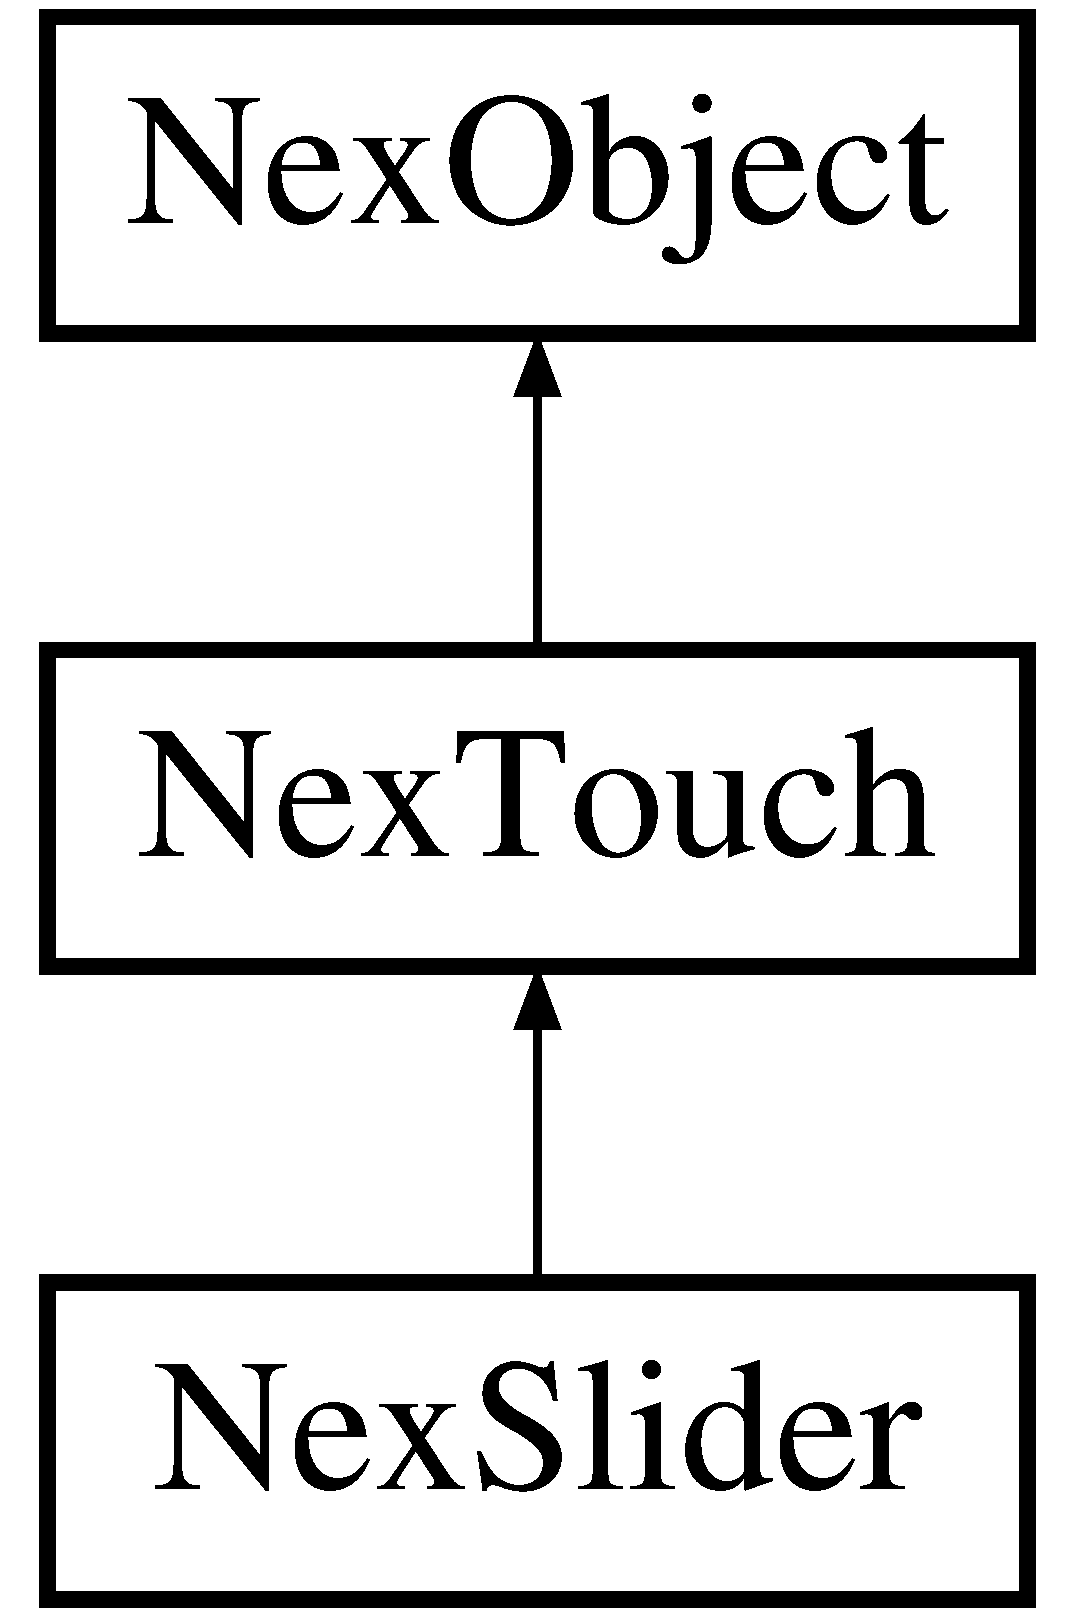
\includegraphics[height=3.000000cm]{class_nex_slider}
\end{center}
\end{figure}
\subsection*{Public Member Functions}
\begin{DoxyCompactItemize}
\item 
\hyperlink{class_nex_slider_a00c5678209c936e9a57c14b6e2384774}{Nex\+Slider} (uint8\+\_\+t pid, uint8\+\_\+t cid, const char $\ast$name)
\item 
bool \hyperlink{class_nex_slider_a384d5488b421efd6affbfd32f45bb107}{get\+Value} (uint32\+\_\+t $\ast$number)
\item 
bool \hyperlink{class_nex_slider_a3f325bda4db913e302e94a4b25de7b5f}{set\+Value} (uint32\+\_\+t number)
\item 
uint32\+\_\+t \hyperlink{class_nex_slider_a1cf49184702852c0623a695f4b62b1ed}{Get\+\_\+background\+\_\+color\+\_\+bco} (uint32\+\_\+t $\ast$number)
\item 
bool \hyperlink{class_nex_slider_ac22c66fecb8cf03d554c3c86e6e798d5}{Set\+\_\+background\+\_\+color\+\_\+bco} (uint32\+\_\+t number)
\item 
uint32\+\_\+t \hyperlink{class_nex_slider_aa6361627b3c66ee7a569b5cfec4ce562}{Get\+\_\+font\+\_\+color\+\_\+pco} (uint32\+\_\+t $\ast$number)
\item 
bool \hyperlink{class_nex_slider_acc766d430c7a663846e4da6e1bacf76c}{Set\+\_\+font\+\_\+color\+\_\+pco} (uint32\+\_\+t number)
\item 
uint32\+\_\+t \hyperlink{class_nex_slider_a6adbc43b663e3542a92641c406db23ad}{Get\+\_\+pointer\+\_\+thickness\+\_\+wid} (uint32\+\_\+t $\ast$number)
\item 
bool \hyperlink{class_nex_slider_a6b91c1f7fddf7ea1b62c406453110ead}{Set\+\_\+pointer\+\_\+thickness\+\_\+wid} (uint32\+\_\+t number)
\item 
uint32\+\_\+t \hyperlink{class_nex_slider_a680c31b1aa2dc48a1193c9d8fb3cd487}{Get\+\_\+cursor\+\_\+height\+\_\+hig} (uint32\+\_\+t $\ast$number)
\item 
bool \hyperlink{class_nex_slider_a603cf3685c6d843261d8552030af9f22}{Set\+\_\+cursor\+\_\+height\+\_\+hig} (uint32\+\_\+t number)
\item 
uint32\+\_\+t \hyperlink{class_nex_slider_abf1b50605feb0ac2b381d1148795f0d9}{get\+Maxval} (uint32\+\_\+t $\ast$number)
\item 
bool \hyperlink{class_nex_slider_a5a1c65a9f2e21a624b78d5817d695503}{set\+Maxval} (uint32\+\_\+t number)
\item 
uint32\+\_\+t \hyperlink{class_nex_slider_ab98752f15d56dc04de102c0c2180ea11}{get\+Minval} (uint32\+\_\+t $\ast$number)
\item 
bool \hyperlink{class_nex_slider_ad38503fd3a6bfe3eaaa57764ac90f244}{set\+Minval} (uint32\+\_\+t number)
\end{DoxyCompactItemize}
\subsection*{Additional Inherited Members}


\subsection{Detailed Description}
\hyperlink{class_nex_slider}{Nex\+Slider} component. 

\subsection{Constructor \& Destructor Documentation}
\hypertarget{class_nex_slider_a00c5678209c936e9a57c14b6e2384774}{\index{Nex\+Slider@{Nex\+Slider}!Nex\+Slider@{Nex\+Slider}}
\index{Nex\+Slider@{Nex\+Slider}!Nex\+Slider@{Nex\+Slider}}
\subsubsection[{Nex\+Slider}]{\setlength{\rightskip}{0pt plus 5cm}Nex\+Slider\+::\+Nex\+Slider (
\begin{DoxyParamCaption}
\item[{uint8\+\_\+t}]{pid, }
\item[{uint8\+\_\+t}]{cid, }
\item[{const char $\ast$}]{name}
\end{DoxyParamCaption}
)}}\label{class_nex_slider_a00c5678209c936e9a57c14b6e2384774}




Constructor.


\begin{DoxyParams}{Parameters}
{\em pid} & -\/ page id. \\
\hline
{\em cid} & -\/ component id. \\
\hline
{\em name} & -\/ pointer to an unique name in range of all components. \\
\hline
\end{DoxyParams}


\subsection{Member Function Documentation}
\hypertarget{class_nex_slider_a1cf49184702852c0623a695f4b62b1ed}{\index{Nex\+Slider@{Nex\+Slider}!Get\+\_\+background\+\_\+color\+\_\+bco@{Get\+\_\+background\+\_\+color\+\_\+bco}}
\index{Get\+\_\+background\+\_\+color\+\_\+bco@{Get\+\_\+background\+\_\+color\+\_\+bco}!Nex\+Slider@{Nex\+Slider}}
\subsubsection[{Get\+\_\+background\+\_\+color\+\_\+bco}]{\setlength{\rightskip}{0pt plus 5cm}uint32\+\_\+t Nex\+Slider\+::\+Get\+\_\+background\+\_\+color\+\_\+bco (
\begin{DoxyParamCaption}
\item[{uint32\+\_\+t $\ast$}]{number}
\end{DoxyParamCaption}
)}}\label{class_nex_slider_a1cf49184702852c0623a695f4b62b1ed}
Get bco attribute of component


\begin{DoxyParams}{Parameters}
{\em number} & -\/ buffer storing data retur \\
\hline
\end{DoxyParams}
\begin{DoxyReturn}{Returns}
the length of the data 
\end{DoxyReturn}
\hypertarget{class_nex_slider_a680c31b1aa2dc48a1193c9d8fb3cd487}{\index{Nex\+Slider@{Nex\+Slider}!Get\+\_\+cursor\+\_\+height\+\_\+hig@{Get\+\_\+cursor\+\_\+height\+\_\+hig}}
\index{Get\+\_\+cursor\+\_\+height\+\_\+hig@{Get\+\_\+cursor\+\_\+height\+\_\+hig}!Nex\+Slider@{Nex\+Slider}}
\subsubsection[{Get\+\_\+cursor\+\_\+height\+\_\+hig}]{\setlength{\rightskip}{0pt plus 5cm}uint32\+\_\+t Nex\+Slider\+::\+Get\+\_\+cursor\+\_\+height\+\_\+hig (
\begin{DoxyParamCaption}
\item[{uint32\+\_\+t $\ast$}]{number}
\end{DoxyParamCaption}
)}}\label{class_nex_slider_a680c31b1aa2dc48a1193c9d8fb3cd487}
Get hig attribute of component


\begin{DoxyParams}{Parameters}
{\em number} & -\/ buffer storing data retur \\
\hline
\end{DoxyParams}
\begin{DoxyReturn}{Returns}
the length of the data 
\end{DoxyReturn}
\hypertarget{class_nex_slider_aa6361627b3c66ee7a569b5cfec4ce562}{\index{Nex\+Slider@{Nex\+Slider}!Get\+\_\+font\+\_\+color\+\_\+pco@{Get\+\_\+font\+\_\+color\+\_\+pco}}
\index{Get\+\_\+font\+\_\+color\+\_\+pco@{Get\+\_\+font\+\_\+color\+\_\+pco}!Nex\+Slider@{Nex\+Slider}}
\subsubsection[{Get\+\_\+font\+\_\+color\+\_\+pco}]{\setlength{\rightskip}{0pt plus 5cm}uint32\+\_\+t Nex\+Slider\+::\+Get\+\_\+font\+\_\+color\+\_\+pco (
\begin{DoxyParamCaption}
\item[{uint32\+\_\+t $\ast$}]{number}
\end{DoxyParamCaption}
)}}\label{class_nex_slider_aa6361627b3c66ee7a569b5cfec4ce562}
Get pco attribute of component


\begin{DoxyParams}{Parameters}
{\em number} & -\/ buffer storing data retur \\
\hline
\end{DoxyParams}
\begin{DoxyReturn}{Returns}
the length of the data 
\end{DoxyReturn}
\hypertarget{class_nex_slider_a6adbc43b663e3542a92641c406db23ad}{\index{Nex\+Slider@{Nex\+Slider}!Get\+\_\+pointer\+\_\+thickness\+\_\+wid@{Get\+\_\+pointer\+\_\+thickness\+\_\+wid}}
\index{Get\+\_\+pointer\+\_\+thickness\+\_\+wid@{Get\+\_\+pointer\+\_\+thickness\+\_\+wid}!Nex\+Slider@{Nex\+Slider}}
\subsubsection[{Get\+\_\+pointer\+\_\+thickness\+\_\+wid}]{\setlength{\rightskip}{0pt plus 5cm}uint32\+\_\+t Nex\+Slider\+::\+Get\+\_\+pointer\+\_\+thickness\+\_\+wid (
\begin{DoxyParamCaption}
\item[{uint32\+\_\+t $\ast$}]{number}
\end{DoxyParamCaption}
)}}\label{class_nex_slider_a6adbc43b663e3542a92641c406db23ad}
Get wid attribute of component


\begin{DoxyParams}{Parameters}
{\em number} & -\/ buffer storing data retur \\
\hline
\end{DoxyParams}
\begin{DoxyReturn}{Returns}
the length of the data 
\end{DoxyReturn}
\hypertarget{class_nex_slider_abf1b50605feb0ac2b381d1148795f0d9}{\index{Nex\+Slider@{Nex\+Slider}!get\+Maxval@{get\+Maxval}}
\index{get\+Maxval@{get\+Maxval}!Nex\+Slider@{Nex\+Slider}}
\subsubsection[{get\+Maxval}]{\setlength{\rightskip}{0pt plus 5cm}uint32\+\_\+t Nex\+Slider\+::get\+Maxval (
\begin{DoxyParamCaption}
\item[{uint32\+\_\+t $\ast$}]{number}
\end{DoxyParamCaption}
)}}\label{class_nex_slider_abf1b50605feb0ac2b381d1148795f0d9}
Get maxval attribute of component


\begin{DoxyParams}{Parameters}
{\em number} & -\/ buffer storing data retur \\
\hline
\end{DoxyParams}
\begin{DoxyReturn}{Returns}
the length of the data 
\end{DoxyReturn}
\hypertarget{class_nex_slider_ab98752f15d56dc04de102c0c2180ea11}{\index{Nex\+Slider@{Nex\+Slider}!get\+Minval@{get\+Minval}}
\index{get\+Minval@{get\+Minval}!Nex\+Slider@{Nex\+Slider}}
\subsubsection[{get\+Minval}]{\setlength{\rightskip}{0pt plus 5cm}uint32\+\_\+t Nex\+Slider\+::get\+Minval (
\begin{DoxyParamCaption}
\item[{uint32\+\_\+t $\ast$}]{number}
\end{DoxyParamCaption}
)}}\label{class_nex_slider_ab98752f15d56dc04de102c0c2180ea11}
Get minval attribute of component


\begin{DoxyParams}{Parameters}
{\em number} & -\/ buffer storing data retur \\
\hline
\end{DoxyParams}
\begin{DoxyReturn}{Returns}
the length of the data 
\end{DoxyReturn}
\hypertarget{class_nex_slider_a384d5488b421efd6affbfd32f45bb107}{\index{Nex\+Slider@{Nex\+Slider}!get\+Value@{get\+Value}}
\index{get\+Value@{get\+Value}!Nex\+Slider@{Nex\+Slider}}
\subsubsection[{get\+Value}]{\setlength{\rightskip}{0pt plus 5cm}bool Nex\+Slider\+::get\+Value (
\begin{DoxyParamCaption}
\item[{uint32\+\_\+t $\ast$}]{number}
\end{DoxyParamCaption}
)}}\label{class_nex_slider_a384d5488b421efd6affbfd32f45bb107}
Get the value of slider.


\begin{DoxyParams}{Parameters}
{\em number} & -\/ an output parameter to save the value of slider.\\
\hline
\end{DoxyParams}

\begin{DoxyRetVals}{Return values}
{\em true} & -\/ success. \\
\hline
{\em false} & -\/ failed. \\
\hline
\end{DoxyRetVals}
\hypertarget{class_nex_slider_ac22c66fecb8cf03d554c3c86e6e798d5}{\index{Nex\+Slider@{Nex\+Slider}!Set\+\_\+background\+\_\+color\+\_\+bco@{Set\+\_\+background\+\_\+color\+\_\+bco}}
\index{Set\+\_\+background\+\_\+color\+\_\+bco@{Set\+\_\+background\+\_\+color\+\_\+bco}!Nex\+Slider@{Nex\+Slider}}
\subsubsection[{Set\+\_\+background\+\_\+color\+\_\+bco}]{\setlength{\rightskip}{0pt plus 5cm}bool Nex\+Slider\+::\+Set\+\_\+background\+\_\+color\+\_\+bco (
\begin{DoxyParamCaption}
\item[{uint32\+\_\+t}]{number}
\end{DoxyParamCaption}
)}}\label{class_nex_slider_ac22c66fecb8cf03d554c3c86e6e798d5}
Set bco attribute of component


\begin{DoxyParams}{Parameters}
{\em number} & -\/ To set up the data \\
\hline
\end{DoxyParams}
\begin{DoxyReturn}{Returns}
true if success, false for failure 
\end{DoxyReturn}
\hypertarget{class_nex_slider_a603cf3685c6d843261d8552030af9f22}{\index{Nex\+Slider@{Nex\+Slider}!Set\+\_\+cursor\+\_\+height\+\_\+hig@{Set\+\_\+cursor\+\_\+height\+\_\+hig}}
\index{Set\+\_\+cursor\+\_\+height\+\_\+hig@{Set\+\_\+cursor\+\_\+height\+\_\+hig}!Nex\+Slider@{Nex\+Slider}}
\subsubsection[{Set\+\_\+cursor\+\_\+height\+\_\+hig}]{\setlength{\rightskip}{0pt plus 5cm}bool Nex\+Slider\+::\+Set\+\_\+cursor\+\_\+height\+\_\+hig (
\begin{DoxyParamCaption}
\item[{uint32\+\_\+t}]{number}
\end{DoxyParamCaption}
)}}\label{class_nex_slider_a603cf3685c6d843261d8552030af9f22}
Set hig attribute of component


\begin{DoxyParams}{Parameters}
{\em number} & -\/ To set up the data \\
\hline
\end{DoxyParams}
\begin{DoxyReturn}{Returns}
true if success, false for failure 
\end{DoxyReturn}
\hypertarget{class_nex_slider_acc766d430c7a663846e4da6e1bacf76c}{\index{Nex\+Slider@{Nex\+Slider}!Set\+\_\+font\+\_\+color\+\_\+pco@{Set\+\_\+font\+\_\+color\+\_\+pco}}
\index{Set\+\_\+font\+\_\+color\+\_\+pco@{Set\+\_\+font\+\_\+color\+\_\+pco}!Nex\+Slider@{Nex\+Slider}}
\subsubsection[{Set\+\_\+font\+\_\+color\+\_\+pco}]{\setlength{\rightskip}{0pt plus 5cm}bool Nex\+Slider\+::\+Set\+\_\+font\+\_\+color\+\_\+pco (
\begin{DoxyParamCaption}
\item[{uint32\+\_\+t}]{number}
\end{DoxyParamCaption}
)}}\label{class_nex_slider_acc766d430c7a663846e4da6e1bacf76c}
Set pco attribute of component


\begin{DoxyParams}{Parameters}
{\em number} & -\/ To set up the data \\
\hline
\end{DoxyParams}
\begin{DoxyReturn}{Returns}
true if success, false for failure 
\end{DoxyReturn}
\hypertarget{class_nex_slider_a6b91c1f7fddf7ea1b62c406453110ead}{\index{Nex\+Slider@{Nex\+Slider}!Set\+\_\+pointer\+\_\+thickness\+\_\+wid@{Set\+\_\+pointer\+\_\+thickness\+\_\+wid}}
\index{Set\+\_\+pointer\+\_\+thickness\+\_\+wid@{Set\+\_\+pointer\+\_\+thickness\+\_\+wid}!Nex\+Slider@{Nex\+Slider}}
\subsubsection[{Set\+\_\+pointer\+\_\+thickness\+\_\+wid}]{\setlength{\rightskip}{0pt plus 5cm}bool Nex\+Slider\+::\+Set\+\_\+pointer\+\_\+thickness\+\_\+wid (
\begin{DoxyParamCaption}
\item[{uint32\+\_\+t}]{number}
\end{DoxyParamCaption}
)}}\label{class_nex_slider_a6b91c1f7fddf7ea1b62c406453110ead}
Set wid attribute of component


\begin{DoxyParams}{Parameters}
{\em number} & -\/ To set up the data \\
\hline
\end{DoxyParams}
\begin{DoxyReturn}{Returns}
true if success, false for failure 
\end{DoxyReturn}
\hypertarget{class_nex_slider_a5a1c65a9f2e21a624b78d5817d695503}{\index{Nex\+Slider@{Nex\+Slider}!set\+Maxval@{set\+Maxval}}
\index{set\+Maxval@{set\+Maxval}!Nex\+Slider@{Nex\+Slider}}
\subsubsection[{set\+Maxval}]{\setlength{\rightskip}{0pt plus 5cm}bool Nex\+Slider\+::set\+Maxval (
\begin{DoxyParamCaption}
\item[{uint32\+\_\+t}]{number}
\end{DoxyParamCaption}
)}}\label{class_nex_slider_a5a1c65a9f2e21a624b78d5817d695503}
Set maxval attribute of component


\begin{DoxyParams}{Parameters}
{\em number} & -\/ To set up the data \\
\hline
\end{DoxyParams}
\begin{DoxyReturn}{Returns}
true if success, false for failure 
\end{DoxyReturn}
\hypertarget{class_nex_slider_ad38503fd3a6bfe3eaaa57764ac90f244}{\index{Nex\+Slider@{Nex\+Slider}!set\+Minval@{set\+Minval}}
\index{set\+Minval@{set\+Minval}!Nex\+Slider@{Nex\+Slider}}
\subsubsection[{set\+Minval}]{\setlength{\rightskip}{0pt plus 5cm}bool Nex\+Slider\+::set\+Minval (
\begin{DoxyParamCaption}
\item[{uint32\+\_\+t}]{number}
\end{DoxyParamCaption}
)}}\label{class_nex_slider_ad38503fd3a6bfe3eaaa57764ac90f244}
Set minval attribute of component


\begin{DoxyParams}{Parameters}
{\em number} & -\/ To set up the data \\
\hline
\end{DoxyParams}
\begin{DoxyReturn}{Returns}
true if success, false for failure 
\end{DoxyReturn}
\hypertarget{class_nex_slider_a3f325bda4db913e302e94a4b25de7b5f}{\index{Nex\+Slider@{Nex\+Slider}!set\+Value@{set\+Value}}
\index{set\+Value@{set\+Value}!Nex\+Slider@{Nex\+Slider}}
\subsubsection[{set\+Value}]{\setlength{\rightskip}{0pt plus 5cm}bool Nex\+Slider\+::set\+Value (
\begin{DoxyParamCaption}
\item[{uint32\+\_\+t}]{number}
\end{DoxyParamCaption}
)}}\label{class_nex_slider_a3f325bda4db913e302e94a4b25de7b5f}
Set the value of slider.


\begin{DoxyParams}{Parameters}
{\em number} & -\/ the value of slider.\\
\hline
\end{DoxyParams}

\begin{DoxyRetVals}{Return values}
{\em true} & -\/ success. \\
\hline
{\em false} & -\/ failed. \\
\hline
\end{DoxyRetVals}


The documentation for this class was generated from the following files\+:\begin{DoxyCompactItemize}
\item 
\hyperlink{_nex_slider_8h}{Nex\+Slider.\+h}\item 
\hyperlink{_nex_slider_8cpp}{Nex\+Slider.\+cpp}\end{DoxyCompactItemize}

\hypertarget{class_nex_text}{\section{Nex\+Text Class Reference}
\label{class_nex_text}\index{Nex\+Text@{Nex\+Text}}
}


{\ttfamily \#include $<$Nex\+Text.\+h$>$}

Inheritance diagram for Nex\+Text\+:\begin{figure}[H]
\begin{center}
\leavevmode
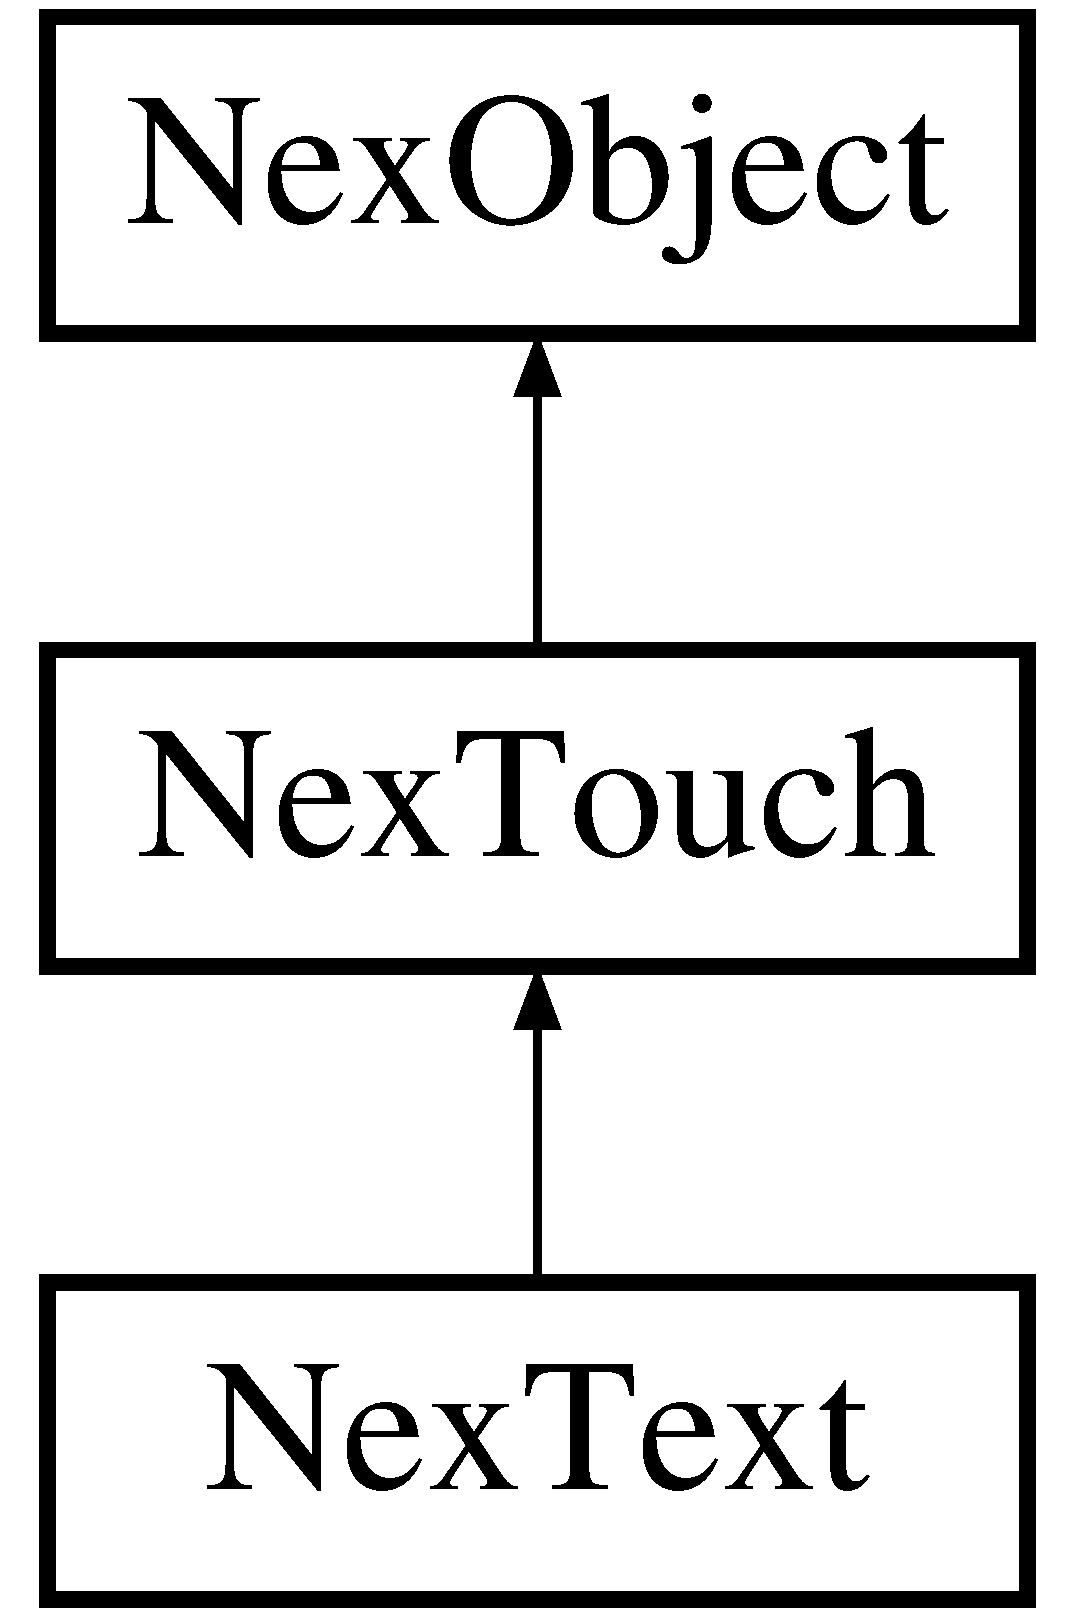
\includegraphics[height=3.000000cm]{class_nex_text}
\end{center}
\end{figure}
\subsection*{Public Member Functions}
\begin{DoxyCompactItemize}
\item 
\hyperlink{class_nex_text_a38b4dd752d39bfda4ef7642b43ded91a}{Nex\+Text} (uint8\+\_\+t pid, uint8\+\_\+t cid, const char $\ast$name)
\item 
uint16\+\_\+t \hyperlink{class_nex_text_a9cf417b2f25df2872492c55bdc9f5b30}{get\+Text} (char $\ast$buffer, uint16\+\_\+t len)
\item 
bool \hyperlink{class_nex_text_a19589b32c981436a1bbcfe407bc766e3}{set\+Text} (const char $\ast$buffer)
\item 
uint32\+\_\+t \hyperlink{class_nex_text_aec8d21665688ba80f3136a1f5e23fef5}{Get\+\_\+background\+\_\+color\+\_\+bco} (uint32\+\_\+t $\ast$number)
\item 
bool \hyperlink{class_nex_text_a1b1586e5e66d76a4f8f5c40b0986f471}{Set\+\_\+background\+\_\+color\+\_\+bco} (uint32\+\_\+t number)
\item 
uint32\+\_\+t \hyperlink{class_nex_text_a860af363c6de6180ef356cad31936185}{Get\+\_\+font\+\_\+color\+\_\+pco} (uint32\+\_\+t $\ast$number)
\item 
bool \hyperlink{class_nex_text_ab59df7e777198eefb422ba2081d0cfce}{Set\+\_\+font\+\_\+color\+\_\+pco} (uint32\+\_\+t number)
\item 
uint32\+\_\+t \hyperlink{class_nex_text_a510a937a104b41859badc220a8ba39fb}{Get\+\_\+place\+\_\+xcen} (uint32\+\_\+t $\ast$number)
\item 
bool \hyperlink{class_nex_text_ab94a4b8505a9bfdf8fb4cb8cb32a1763}{Set\+\_\+place\+\_\+xcen} (uint32\+\_\+t number)
\item 
uint32\+\_\+t \hyperlink{class_nex_text_a9bd42732e37497a8fb44ece94b39285c}{Get\+\_\+place\+\_\+ycen} (uint32\+\_\+t $\ast$number)
\item 
bool \hyperlink{class_nex_text_a0f8ad9780c8145569da6736d0ee494e4}{Set\+\_\+place\+\_\+ycen} (uint32\+\_\+t number)
\item 
uint32\+\_\+t \hyperlink{class_nex_text_adc480199a2b396811aa0c14928b592c8}{get\+Font} (uint32\+\_\+t $\ast$number)
\item 
bool \hyperlink{class_nex_text_a5dd7fdda945a76033ef8fe8dc68e3e52}{set\+Font} (uint32\+\_\+t number)
\item 
uint32\+\_\+t \hyperlink{class_nex_text_ae44393fb20ba449bf088dbd0758b4219}{Get\+\_\+background\+\_\+crop\+\_\+picc} (uint32\+\_\+t $\ast$number)
\item 
bool \hyperlink{class_nex_text_a3727463a4fc0e1df978cd8fc7d1103ed}{Set\+\_\+background\+\_\+crop\+\_\+picc} (uint32\+\_\+t number)
\item 
uint32\+\_\+t \hyperlink{class_nex_text_aed07b3988fe2c4ec332727bb245e49a5}{Get\+\_\+background\+\_\+image\+\_\+pic} (uint32\+\_\+t $\ast$number)
\item 
bool \hyperlink{class_nex_text_ab2c85ac7d5184e124b0cd724028c1915}{Set\+\_\+background\+\_\+image\+\_\+pic} (uint32\+\_\+t number)
\end{DoxyCompactItemize}
\subsection*{Additional Inherited Members}


\subsection{Detailed Description}
\hyperlink{class_nex_text}{Nex\+Text} component. 

\subsection{Constructor \& Destructor Documentation}
\hypertarget{class_nex_text_a38b4dd752d39bfda4ef7642b43ded91a}{\index{Nex\+Text@{Nex\+Text}!Nex\+Text@{Nex\+Text}}
\index{Nex\+Text@{Nex\+Text}!Nex\+Text@{Nex\+Text}}
\subsubsection[{Nex\+Text}]{\setlength{\rightskip}{0pt plus 5cm}Nex\+Text\+::\+Nex\+Text (
\begin{DoxyParamCaption}
\item[{uint8\+\_\+t}]{pid, }
\item[{uint8\+\_\+t}]{cid, }
\item[{const char $\ast$}]{name}
\end{DoxyParamCaption}
)}}\label{class_nex_text_a38b4dd752d39bfda4ef7642b43ded91a}




Constructor.


\begin{DoxyParams}{Parameters}
{\em pid} & -\/ page id. \\
\hline
{\em cid} & -\/ component id. \\
\hline
{\em name} & -\/ pointer to an unique name in range of all components. \\
\hline
\end{DoxyParams}


\subsection{Member Function Documentation}
\hypertarget{class_nex_text_aec8d21665688ba80f3136a1f5e23fef5}{\index{Nex\+Text@{Nex\+Text}!Get\+\_\+background\+\_\+color\+\_\+bco@{Get\+\_\+background\+\_\+color\+\_\+bco}}
\index{Get\+\_\+background\+\_\+color\+\_\+bco@{Get\+\_\+background\+\_\+color\+\_\+bco}!Nex\+Text@{Nex\+Text}}
\subsubsection[{Get\+\_\+background\+\_\+color\+\_\+bco}]{\setlength{\rightskip}{0pt plus 5cm}uint32\+\_\+t Nex\+Text\+::\+Get\+\_\+background\+\_\+color\+\_\+bco (
\begin{DoxyParamCaption}
\item[{uint32\+\_\+t $\ast$}]{number}
\end{DoxyParamCaption}
)}}\label{class_nex_text_aec8d21665688ba80f3136a1f5e23fef5}
Get bco attribute of component


\begin{DoxyParams}{Parameters}
{\em number} & -\/ buffer storing data retur \\
\hline
\end{DoxyParams}
\begin{DoxyReturn}{Returns}
the length of the data 
\end{DoxyReturn}
\hypertarget{class_nex_text_ae44393fb20ba449bf088dbd0758b4219}{\index{Nex\+Text@{Nex\+Text}!Get\+\_\+background\+\_\+crop\+\_\+picc@{Get\+\_\+background\+\_\+crop\+\_\+picc}}
\index{Get\+\_\+background\+\_\+crop\+\_\+picc@{Get\+\_\+background\+\_\+crop\+\_\+picc}!Nex\+Text@{Nex\+Text}}
\subsubsection[{Get\+\_\+background\+\_\+crop\+\_\+picc}]{\setlength{\rightskip}{0pt plus 5cm}uint32\+\_\+t Nex\+Text\+::\+Get\+\_\+background\+\_\+crop\+\_\+picc (
\begin{DoxyParamCaption}
\item[{uint32\+\_\+t $\ast$}]{number}
\end{DoxyParamCaption}
)}}\label{class_nex_text_ae44393fb20ba449bf088dbd0758b4219}
Get picc attribute of component


\begin{DoxyParams}{Parameters}
{\em number} & -\/ buffer storing data retur \\
\hline
\end{DoxyParams}
\begin{DoxyReturn}{Returns}
the length of the data 
\end{DoxyReturn}
\hypertarget{class_nex_text_aed07b3988fe2c4ec332727bb245e49a5}{\index{Nex\+Text@{Nex\+Text}!Get\+\_\+background\+\_\+image\+\_\+pic@{Get\+\_\+background\+\_\+image\+\_\+pic}}
\index{Get\+\_\+background\+\_\+image\+\_\+pic@{Get\+\_\+background\+\_\+image\+\_\+pic}!Nex\+Text@{Nex\+Text}}
\subsubsection[{Get\+\_\+background\+\_\+image\+\_\+pic}]{\setlength{\rightskip}{0pt plus 5cm}uint32\+\_\+t Nex\+Text\+::\+Get\+\_\+background\+\_\+image\+\_\+pic (
\begin{DoxyParamCaption}
\item[{uint32\+\_\+t $\ast$}]{number}
\end{DoxyParamCaption}
)}}\label{class_nex_text_aed07b3988fe2c4ec332727bb245e49a5}
Get pic attribute of component


\begin{DoxyParams}{Parameters}
{\em number} & -\/ buffer storing data retur \\
\hline
\end{DoxyParams}
\begin{DoxyReturn}{Returns}
the length of the data 
\end{DoxyReturn}
\hypertarget{class_nex_text_a860af363c6de6180ef356cad31936185}{\index{Nex\+Text@{Nex\+Text}!Get\+\_\+font\+\_\+color\+\_\+pco@{Get\+\_\+font\+\_\+color\+\_\+pco}}
\index{Get\+\_\+font\+\_\+color\+\_\+pco@{Get\+\_\+font\+\_\+color\+\_\+pco}!Nex\+Text@{Nex\+Text}}
\subsubsection[{Get\+\_\+font\+\_\+color\+\_\+pco}]{\setlength{\rightskip}{0pt plus 5cm}uint32\+\_\+t Nex\+Text\+::\+Get\+\_\+font\+\_\+color\+\_\+pco (
\begin{DoxyParamCaption}
\item[{uint32\+\_\+t $\ast$}]{number}
\end{DoxyParamCaption}
)}}\label{class_nex_text_a860af363c6de6180ef356cad31936185}
Get pco attribute of component


\begin{DoxyParams}{Parameters}
{\em number} & -\/ buffer storing data retur \\
\hline
\end{DoxyParams}
\begin{DoxyReturn}{Returns}
the length of the data 
\end{DoxyReturn}
\hypertarget{class_nex_text_a510a937a104b41859badc220a8ba39fb}{\index{Nex\+Text@{Nex\+Text}!Get\+\_\+place\+\_\+xcen@{Get\+\_\+place\+\_\+xcen}}
\index{Get\+\_\+place\+\_\+xcen@{Get\+\_\+place\+\_\+xcen}!Nex\+Text@{Nex\+Text}}
\subsubsection[{Get\+\_\+place\+\_\+xcen}]{\setlength{\rightskip}{0pt plus 5cm}uint32\+\_\+t Nex\+Text\+::\+Get\+\_\+place\+\_\+xcen (
\begin{DoxyParamCaption}
\item[{uint32\+\_\+t $\ast$}]{number}
\end{DoxyParamCaption}
)}}\label{class_nex_text_a510a937a104b41859badc220a8ba39fb}
Get xcen attribute of component


\begin{DoxyParams}{Parameters}
{\em number} & -\/ buffer storing data retur \\
\hline
\end{DoxyParams}
\begin{DoxyReturn}{Returns}
the length of the data 
\end{DoxyReturn}
\hypertarget{class_nex_text_a9bd42732e37497a8fb44ece94b39285c}{\index{Nex\+Text@{Nex\+Text}!Get\+\_\+place\+\_\+ycen@{Get\+\_\+place\+\_\+ycen}}
\index{Get\+\_\+place\+\_\+ycen@{Get\+\_\+place\+\_\+ycen}!Nex\+Text@{Nex\+Text}}
\subsubsection[{Get\+\_\+place\+\_\+ycen}]{\setlength{\rightskip}{0pt plus 5cm}uint32\+\_\+t Nex\+Text\+::\+Get\+\_\+place\+\_\+ycen (
\begin{DoxyParamCaption}
\item[{uint32\+\_\+t $\ast$}]{number}
\end{DoxyParamCaption}
)}}\label{class_nex_text_a9bd42732e37497a8fb44ece94b39285c}
Get ycen attribute of component


\begin{DoxyParams}{Parameters}
{\em number} & -\/ buffer storing data retur \\
\hline
\end{DoxyParams}
\begin{DoxyReturn}{Returns}
the length of the data 
\end{DoxyReturn}
\hypertarget{class_nex_text_adc480199a2b396811aa0c14928b592c8}{\index{Nex\+Text@{Nex\+Text}!get\+Font@{get\+Font}}
\index{get\+Font@{get\+Font}!Nex\+Text@{Nex\+Text}}
\subsubsection[{get\+Font}]{\setlength{\rightskip}{0pt plus 5cm}uint32\+\_\+t Nex\+Text\+::get\+Font (
\begin{DoxyParamCaption}
\item[{uint32\+\_\+t $\ast$}]{number}
\end{DoxyParamCaption}
)}}\label{class_nex_text_adc480199a2b396811aa0c14928b592c8}
Get font attribute of component


\begin{DoxyParams}{Parameters}
{\em number} & -\/ buffer storing data retur \\
\hline
\end{DoxyParams}
\begin{DoxyReturn}{Returns}
the length of the data 
\end{DoxyReturn}
\hypertarget{class_nex_text_a9cf417b2f25df2872492c55bdc9f5b30}{\index{Nex\+Text@{Nex\+Text}!get\+Text@{get\+Text}}
\index{get\+Text@{get\+Text}!Nex\+Text@{Nex\+Text}}
\subsubsection[{get\+Text}]{\setlength{\rightskip}{0pt plus 5cm}uint16\+\_\+t Nex\+Text\+::get\+Text (
\begin{DoxyParamCaption}
\item[{char $\ast$}]{buffer, }
\item[{uint16\+\_\+t}]{len}
\end{DoxyParamCaption}
)}}\label{class_nex_text_a9cf417b2f25df2872492c55bdc9f5b30}
Get text attribute of component.


\begin{DoxyParams}{Parameters}
{\em buffer} & -\/ buffer storing text returned. \\
\hline
{\em len} & -\/ length of buffer. \\
\hline
\end{DoxyParams}
\begin{DoxyReturn}{Returns}
The real length of text returned. 
\end{DoxyReturn}
\hypertarget{class_nex_text_a1b1586e5e66d76a4f8f5c40b0986f471}{\index{Nex\+Text@{Nex\+Text}!Set\+\_\+background\+\_\+color\+\_\+bco@{Set\+\_\+background\+\_\+color\+\_\+bco}}
\index{Set\+\_\+background\+\_\+color\+\_\+bco@{Set\+\_\+background\+\_\+color\+\_\+bco}!Nex\+Text@{Nex\+Text}}
\subsubsection[{Set\+\_\+background\+\_\+color\+\_\+bco}]{\setlength{\rightskip}{0pt plus 5cm}bool Nex\+Text\+::\+Set\+\_\+background\+\_\+color\+\_\+bco (
\begin{DoxyParamCaption}
\item[{uint32\+\_\+t}]{number}
\end{DoxyParamCaption}
)}}\label{class_nex_text_a1b1586e5e66d76a4f8f5c40b0986f471}
Set bco attribute of component


\begin{DoxyParams}{Parameters}
{\em number} & -\/ To set up the data \\
\hline
\end{DoxyParams}
\begin{DoxyReturn}{Returns}
true if success, false for failure 
\end{DoxyReturn}
\hypertarget{class_nex_text_a3727463a4fc0e1df978cd8fc7d1103ed}{\index{Nex\+Text@{Nex\+Text}!Set\+\_\+background\+\_\+crop\+\_\+picc@{Set\+\_\+background\+\_\+crop\+\_\+picc}}
\index{Set\+\_\+background\+\_\+crop\+\_\+picc@{Set\+\_\+background\+\_\+crop\+\_\+picc}!Nex\+Text@{Nex\+Text}}
\subsubsection[{Set\+\_\+background\+\_\+crop\+\_\+picc}]{\setlength{\rightskip}{0pt plus 5cm}bool Nex\+Text\+::\+Set\+\_\+background\+\_\+crop\+\_\+picc (
\begin{DoxyParamCaption}
\item[{uint32\+\_\+t}]{number}
\end{DoxyParamCaption}
)}}\label{class_nex_text_a3727463a4fc0e1df978cd8fc7d1103ed}
Set picc attribute of component


\begin{DoxyParams}{Parameters}
{\em number} & -\/ To set up the data \\
\hline
\end{DoxyParams}
\begin{DoxyReturn}{Returns}
true if success, false for failure 
\end{DoxyReturn}
\hypertarget{class_nex_text_ab2c85ac7d5184e124b0cd724028c1915}{\index{Nex\+Text@{Nex\+Text}!Set\+\_\+background\+\_\+image\+\_\+pic@{Set\+\_\+background\+\_\+image\+\_\+pic}}
\index{Set\+\_\+background\+\_\+image\+\_\+pic@{Set\+\_\+background\+\_\+image\+\_\+pic}!Nex\+Text@{Nex\+Text}}
\subsubsection[{Set\+\_\+background\+\_\+image\+\_\+pic}]{\setlength{\rightskip}{0pt plus 5cm}bool Nex\+Text\+::\+Set\+\_\+background\+\_\+image\+\_\+pic (
\begin{DoxyParamCaption}
\item[{uint32\+\_\+t}]{number}
\end{DoxyParamCaption}
)}}\label{class_nex_text_ab2c85ac7d5184e124b0cd724028c1915}
Set pic attribute of component


\begin{DoxyParams}{Parameters}
{\em number} & -\/ To set up the data \\
\hline
\end{DoxyParams}
\begin{DoxyReturn}{Returns}
true if success, false for failure 
\end{DoxyReturn}
\hypertarget{class_nex_text_ab59df7e777198eefb422ba2081d0cfce}{\index{Nex\+Text@{Nex\+Text}!Set\+\_\+font\+\_\+color\+\_\+pco@{Set\+\_\+font\+\_\+color\+\_\+pco}}
\index{Set\+\_\+font\+\_\+color\+\_\+pco@{Set\+\_\+font\+\_\+color\+\_\+pco}!Nex\+Text@{Nex\+Text}}
\subsubsection[{Set\+\_\+font\+\_\+color\+\_\+pco}]{\setlength{\rightskip}{0pt plus 5cm}bool Nex\+Text\+::\+Set\+\_\+font\+\_\+color\+\_\+pco (
\begin{DoxyParamCaption}
\item[{uint32\+\_\+t}]{number}
\end{DoxyParamCaption}
)}}\label{class_nex_text_ab59df7e777198eefb422ba2081d0cfce}
Set pco attribute of component


\begin{DoxyParams}{Parameters}
{\em number} & -\/ To set up the data \\
\hline
\end{DoxyParams}
\begin{DoxyReturn}{Returns}
true if success, false for failure 
\end{DoxyReturn}
\hypertarget{class_nex_text_ab94a4b8505a9bfdf8fb4cb8cb32a1763}{\index{Nex\+Text@{Nex\+Text}!Set\+\_\+place\+\_\+xcen@{Set\+\_\+place\+\_\+xcen}}
\index{Set\+\_\+place\+\_\+xcen@{Set\+\_\+place\+\_\+xcen}!Nex\+Text@{Nex\+Text}}
\subsubsection[{Set\+\_\+place\+\_\+xcen}]{\setlength{\rightskip}{0pt plus 5cm}bool Nex\+Text\+::\+Set\+\_\+place\+\_\+xcen (
\begin{DoxyParamCaption}
\item[{uint32\+\_\+t}]{number}
\end{DoxyParamCaption}
)}}\label{class_nex_text_ab94a4b8505a9bfdf8fb4cb8cb32a1763}
Set xcen attribute of component


\begin{DoxyParams}{Parameters}
{\em number} & -\/ To set up the data \\
\hline
\end{DoxyParams}
\begin{DoxyReturn}{Returns}
true if success, false for failure 
\end{DoxyReturn}
\hypertarget{class_nex_text_a0f8ad9780c8145569da6736d0ee494e4}{\index{Nex\+Text@{Nex\+Text}!Set\+\_\+place\+\_\+ycen@{Set\+\_\+place\+\_\+ycen}}
\index{Set\+\_\+place\+\_\+ycen@{Set\+\_\+place\+\_\+ycen}!Nex\+Text@{Nex\+Text}}
\subsubsection[{Set\+\_\+place\+\_\+ycen}]{\setlength{\rightskip}{0pt plus 5cm}bool Nex\+Text\+::\+Set\+\_\+place\+\_\+ycen (
\begin{DoxyParamCaption}
\item[{uint32\+\_\+t}]{number}
\end{DoxyParamCaption}
)}}\label{class_nex_text_a0f8ad9780c8145569da6736d0ee494e4}
Set ycen attribute of component


\begin{DoxyParams}{Parameters}
{\em number} & -\/ To set up the data \\
\hline
\end{DoxyParams}
\begin{DoxyReturn}{Returns}
true if success, false for failure 
\end{DoxyReturn}
\hypertarget{class_nex_text_a5dd7fdda945a76033ef8fe8dc68e3e52}{\index{Nex\+Text@{Nex\+Text}!set\+Font@{set\+Font}}
\index{set\+Font@{set\+Font}!Nex\+Text@{Nex\+Text}}
\subsubsection[{set\+Font}]{\setlength{\rightskip}{0pt plus 5cm}bool Nex\+Text\+::set\+Font (
\begin{DoxyParamCaption}
\item[{uint32\+\_\+t}]{number}
\end{DoxyParamCaption}
)}}\label{class_nex_text_a5dd7fdda945a76033ef8fe8dc68e3e52}
Set font attribute of component


\begin{DoxyParams}{Parameters}
{\em number} & -\/ To set up the data \\
\hline
\end{DoxyParams}
\begin{DoxyReturn}{Returns}
true if success, false for failure 
\end{DoxyReturn}
\hypertarget{class_nex_text_a19589b32c981436a1bbcfe407bc766e3}{\index{Nex\+Text@{Nex\+Text}!set\+Text@{set\+Text}}
\index{set\+Text@{set\+Text}!Nex\+Text@{Nex\+Text}}
\subsubsection[{set\+Text}]{\setlength{\rightskip}{0pt plus 5cm}bool Nex\+Text\+::set\+Text (
\begin{DoxyParamCaption}
\item[{const char $\ast$}]{buffer}
\end{DoxyParamCaption}
)}}\label{class_nex_text_a19589b32c981436a1bbcfe407bc766e3}
Set text attribute of component.


\begin{DoxyParams}{Parameters}
{\em buffer} & -\/ text buffer terminated with '\textbackslash{}0'. \\
\hline
\end{DoxyParams}
\begin{DoxyReturn}{Returns}
true if success, false for failure. 
\end{DoxyReturn}


The documentation for this class was generated from the following files\+:\begin{DoxyCompactItemize}
\item 
\hyperlink{_nex_text_8h}{Nex\+Text.\+h}\item 
\hyperlink{_nex_text_8cpp}{Nex\+Text.\+cpp}\end{DoxyCompactItemize}

\hypertarget{class_nex_timer}{\section{Nex\+Timer Class Reference}
\label{class_nex_timer}\index{Nex\+Timer@{Nex\+Timer}}
}


{\ttfamily \#include $<$Nex\+Timer.\+h$>$}

Inheritance diagram for Nex\+Timer\+:\begin{figure}[H]
\begin{center}
\leavevmode
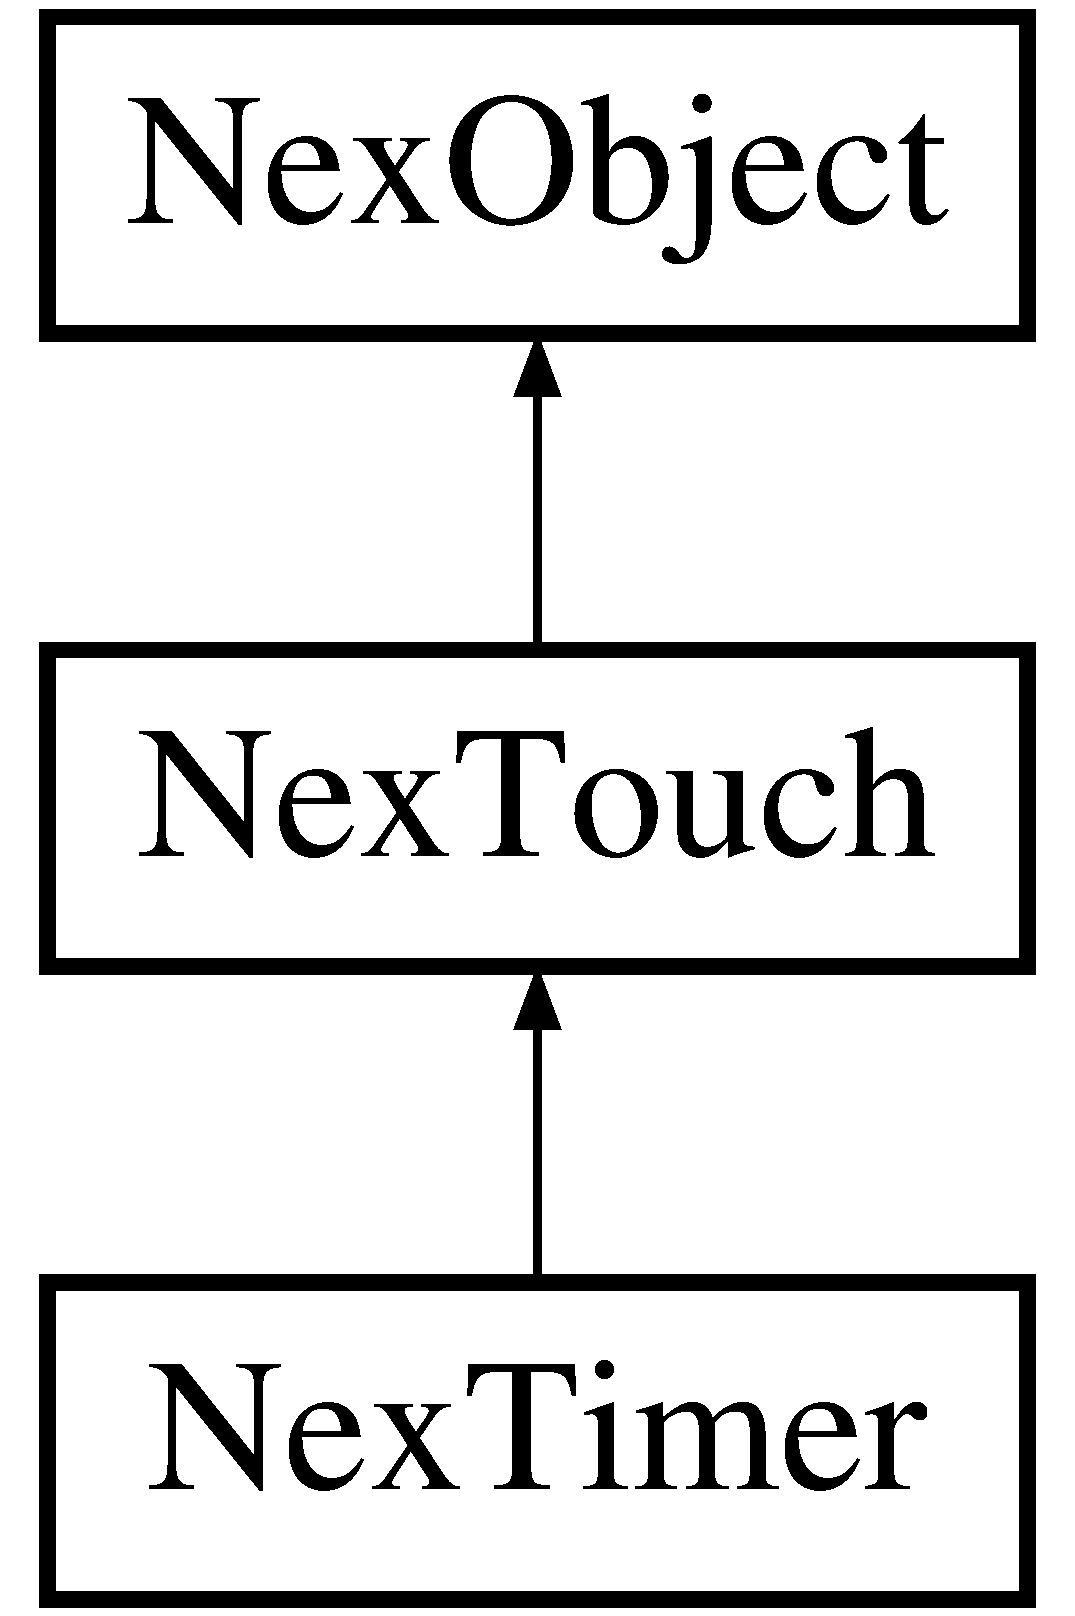
\includegraphics[height=3.000000cm]{class_nex_timer}
\end{center}
\end{figure}
\subsection*{Public Member Functions}
\begin{DoxyCompactItemize}
\item 
\hyperlink{class_nex_timer_a5cb6cdcf0d7e46723364d486d4dcd650}{Nex\+Timer} (uint8\+\_\+t pid, uint8\+\_\+t cid, const char $\ast$name)
\item 
void \hyperlink{class_nex_timer_ae6f1ae95ef40b8bc6f482185b1ec5175}{attach\+Timer} (\hyperlink{group___touch_event_ga162dea47b078e8878d10d6981a9dd0c6}{Nex\+Touch\+Event\+Cb} timer, void $\ast$ptr=N\+U\+L\+L)
\item 
void \hyperlink{class_nex_timer_a365d08df4623ce8a146e73ff9204d5cb}{detach\+Timer} (void)
\item 
bool \hyperlink{class_nex_timer_afd95e7490e28e2a36437be608f26b40e}{get\+Cycle} (uint32\+\_\+t $\ast$number)
\item 
bool \hyperlink{class_nex_timer_acf20f76949ed43f05b1c33613dabcb01}{set\+Cycle} (uint32\+\_\+t number)
\item 
bool \hyperlink{class_nex_timer_a01c146befad40fc0321891ac69e75710}{enable} (void)
\item 
bool \hyperlink{class_nex_timer_ae016d7d39ede6cf813221b26691809f1}{disable} (void)
\item 
uint32\+\_\+t \hyperlink{class_nex_timer_ae186b1c014e8bf67036f8a5faf73ae67}{Get\+\_\+cycle\+\_\+tim} (uint32\+\_\+t $\ast$number)
\item 
bool \hyperlink{class_nex_timer_a30829813c0c42680c1f7bcf5fc5b7c8b}{Set\+\_\+cycle\+\_\+tim} (uint32\+\_\+t number)
\end{DoxyCompactItemize}
\subsection*{Additional Inherited Members}


\subsection{Detailed Description}
\hyperlink{class_nex_timer}{Nex\+Timer} component.

Commonly, you want to do something after set timer cycle and enable it,and the cycle value must be greater than 50 

\subsection{Constructor \& Destructor Documentation}
\hypertarget{class_nex_timer_a5cb6cdcf0d7e46723364d486d4dcd650}{\index{Nex\+Timer@{Nex\+Timer}!Nex\+Timer@{Nex\+Timer}}
\index{Nex\+Timer@{Nex\+Timer}!Nex\+Timer@{Nex\+Timer}}
\subsubsection[{Nex\+Timer}]{\setlength{\rightskip}{0pt plus 5cm}Nex\+Timer\+::\+Nex\+Timer (
\begin{DoxyParamCaption}
\item[{uint8\+\_\+t}]{pid, }
\item[{uint8\+\_\+t}]{cid, }
\item[{const char $\ast$}]{name}
\end{DoxyParamCaption}
)}}\label{class_nex_timer_a5cb6cdcf0d7e46723364d486d4dcd650}




Constructor.


\begin{DoxyParams}{Parameters}
{\em pid} & -\/ page id. \\
\hline
{\em cid} & -\/ component id. \\
\hline
{\em name} & -\/ pointer to an unique name in range of all components. \\
\hline
\end{DoxyParams}


\subsection{Member Function Documentation}
\hypertarget{class_nex_timer_ae6f1ae95ef40b8bc6f482185b1ec5175}{\index{Nex\+Timer@{Nex\+Timer}!attach\+Timer@{attach\+Timer}}
\index{attach\+Timer@{attach\+Timer}!Nex\+Timer@{Nex\+Timer}}
\subsubsection[{attach\+Timer}]{\setlength{\rightskip}{0pt plus 5cm}void Nex\+Timer\+::attach\+Timer (
\begin{DoxyParamCaption}
\item[{{\bf Nex\+Touch\+Event\+Cb}}]{timer, }
\item[{void $\ast$}]{ptr = {\ttfamily NULL}}
\end{DoxyParamCaption}
)}}\label{class_nex_timer_ae6f1ae95ef40b8bc6f482185b1ec5175}
Attach an callback function of timer respond event.


\begin{DoxyParams}{Parameters}
{\em timer} & -\/ callback called with ptr when a timer respond event occurs. \\
\hline
{\em ptr} & -\/ parameter passed into push\mbox{[}default\+:N\+U\+L\+L\mbox{]}. \\
\hline
\end{DoxyParams}
\begin{DoxyReturn}{Returns}
none.
\end{DoxyReturn}
\begin{DoxyNote}{Note}
If calling this method multiply, the last call is valid. 
\end{DoxyNote}
\hypertarget{class_nex_timer_a365d08df4623ce8a146e73ff9204d5cb}{\index{Nex\+Timer@{Nex\+Timer}!detach\+Timer@{detach\+Timer}}
\index{detach\+Timer@{detach\+Timer}!Nex\+Timer@{Nex\+Timer}}
\subsubsection[{detach\+Timer}]{\setlength{\rightskip}{0pt plus 5cm}void Nex\+Timer\+::detach\+Timer (
\begin{DoxyParamCaption}
\item[{void}]{}
\end{DoxyParamCaption}
)}}\label{class_nex_timer_a365d08df4623ce8a146e73ff9204d5cb}
Detach an callback function.

\begin{DoxyReturn}{Returns}
none. 
\end{DoxyReturn}
\hypertarget{class_nex_timer_ae016d7d39ede6cf813221b26691809f1}{\index{Nex\+Timer@{Nex\+Timer}!disable@{disable}}
\index{disable@{disable}!Nex\+Timer@{Nex\+Timer}}
\subsubsection[{disable}]{\setlength{\rightskip}{0pt plus 5cm}bool Nex\+Timer\+::disable (
\begin{DoxyParamCaption}
\item[{void}]{}
\end{DoxyParamCaption}
)}}\label{class_nex_timer_ae016d7d39ede6cf813221b26691809f1}
contorl timer disable.


\begin{DoxyRetVals}{Return values}
{\em true} & -\/ success. \\
\hline
{\em false} & -\/ failed. \\
\hline
\end{DoxyRetVals}
\hypertarget{class_nex_timer_a01c146befad40fc0321891ac69e75710}{\index{Nex\+Timer@{Nex\+Timer}!enable@{enable}}
\index{enable@{enable}!Nex\+Timer@{Nex\+Timer}}
\subsubsection[{enable}]{\setlength{\rightskip}{0pt plus 5cm}bool Nex\+Timer\+::enable (
\begin{DoxyParamCaption}
\item[{void}]{}
\end{DoxyParamCaption}
)}}\label{class_nex_timer_a01c146befad40fc0321891ac69e75710}
contorl timer enable.


\begin{DoxyRetVals}{Return values}
{\em true} & -\/ success. \\
\hline
{\em false} & -\/ failed. \\
\hline
\end{DoxyRetVals}
\hypertarget{class_nex_timer_ae186b1c014e8bf67036f8a5faf73ae67}{\index{Nex\+Timer@{Nex\+Timer}!Get\+\_\+cycle\+\_\+tim@{Get\+\_\+cycle\+\_\+tim}}
\index{Get\+\_\+cycle\+\_\+tim@{Get\+\_\+cycle\+\_\+tim}!Nex\+Timer@{Nex\+Timer}}
\subsubsection[{Get\+\_\+cycle\+\_\+tim}]{\setlength{\rightskip}{0pt plus 5cm}uint32\+\_\+t Nex\+Timer\+::\+Get\+\_\+cycle\+\_\+tim (
\begin{DoxyParamCaption}
\item[{uint32\+\_\+t $\ast$}]{number}
\end{DoxyParamCaption}
)}}\label{class_nex_timer_ae186b1c014e8bf67036f8a5faf73ae67}
Get tim attribute of component


\begin{DoxyParams}{Parameters}
{\em number} & -\/ buffer storing data retur \\
\hline
\end{DoxyParams}
\begin{DoxyReturn}{Returns}
the length of the data 
\end{DoxyReturn}
\hypertarget{class_nex_timer_afd95e7490e28e2a36437be608f26b40e}{\index{Nex\+Timer@{Nex\+Timer}!get\+Cycle@{get\+Cycle}}
\index{get\+Cycle@{get\+Cycle}!Nex\+Timer@{Nex\+Timer}}
\subsubsection[{get\+Cycle}]{\setlength{\rightskip}{0pt plus 5cm}bool Nex\+Timer\+::get\+Cycle (
\begin{DoxyParamCaption}
\item[{uint32\+\_\+t $\ast$}]{number}
\end{DoxyParamCaption}
)}}\label{class_nex_timer_afd95e7490e28e2a36437be608f26b40e}
Get the value of timer cycle val.


\begin{DoxyParams}{Parameters}
{\em number} & -\/ an output parameter to save the value of timer cycle.\\
\hline
\end{DoxyParams}

\begin{DoxyRetVals}{Return values}
{\em true} & -\/ success. \\
\hline
{\em false} & -\/ failed. \\
\hline
\end{DoxyRetVals}
\hypertarget{class_nex_timer_a30829813c0c42680c1f7bcf5fc5b7c8b}{\index{Nex\+Timer@{Nex\+Timer}!Set\+\_\+cycle\+\_\+tim@{Set\+\_\+cycle\+\_\+tim}}
\index{Set\+\_\+cycle\+\_\+tim@{Set\+\_\+cycle\+\_\+tim}!Nex\+Timer@{Nex\+Timer}}
\subsubsection[{Set\+\_\+cycle\+\_\+tim}]{\setlength{\rightskip}{0pt plus 5cm}bool Nex\+Timer\+::\+Set\+\_\+cycle\+\_\+tim (
\begin{DoxyParamCaption}
\item[{uint32\+\_\+t}]{number}
\end{DoxyParamCaption}
)}}\label{class_nex_timer_a30829813c0c42680c1f7bcf5fc5b7c8b}
Set tim attribute of component


\begin{DoxyParams}{Parameters}
{\em number} & -\/ To set up the data \\
\hline
\end{DoxyParams}
\begin{DoxyReturn}{Returns}
true if success, false for failure 
\end{DoxyReturn}
\hypertarget{class_nex_timer_acf20f76949ed43f05b1c33613dabcb01}{\index{Nex\+Timer@{Nex\+Timer}!set\+Cycle@{set\+Cycle}}
\index{set\+Cycle@{set\+Cycle}!Nex\+Timer@{Nex\+Timer}}
\subsubsection[{set\+Cycle}]{\setlength{\rightskip}{0pt plus 5cm}bool Nex\+Timer\+::set\+Cycle (
\begin{DoxyParamCaption}
\item[{uint32\+\_\+t}]{number}
\end{DoxyParamCaption}
)}}\label{class_nex_timer_acf20f76949ed43f05b1c33613dabcb01}
Set the value of timer cycle val.


\begin{DoxyParams}{Parameters}
{\em number} & -\/ the value of timer cycle.\\
\hline
\end{DoxyParams}

\begin{DoxyRetVals}{Return values}
{\em true} & -\/ success. \\
\hline
{\em false} & -\/ failed.\\
\hline
\end{DoxyRetVals}
\begin{DoxyWarning}{Warning}
the cycle value must be greater than 50. 
\end{DoxyWarning}


The documentation for this class was generated from the following files\+:\begin{DoxyCompactItemize}
\item 
\hyperlink{_nex_timer_8h}{Nex\+Timer.\+h}\item 
\hyperlink{_nex_timer_8cpp}{Nex\+Timer.\+cpp}\end{DoxyCompactItemize}

\hypertarget{class_nex_touch}{\section{Nex\+Touch Class Reference}
\label{class_nex_touch}\index{Nex\+Touch@{Nex\+Touch}}
}


{\ttfamily \#include $<$Nex\+Touch.\+h$>$}

Inheritance diagram for Nex\+Touch\+:\begin{figure}[H]
\begin{center}
\leavevmode
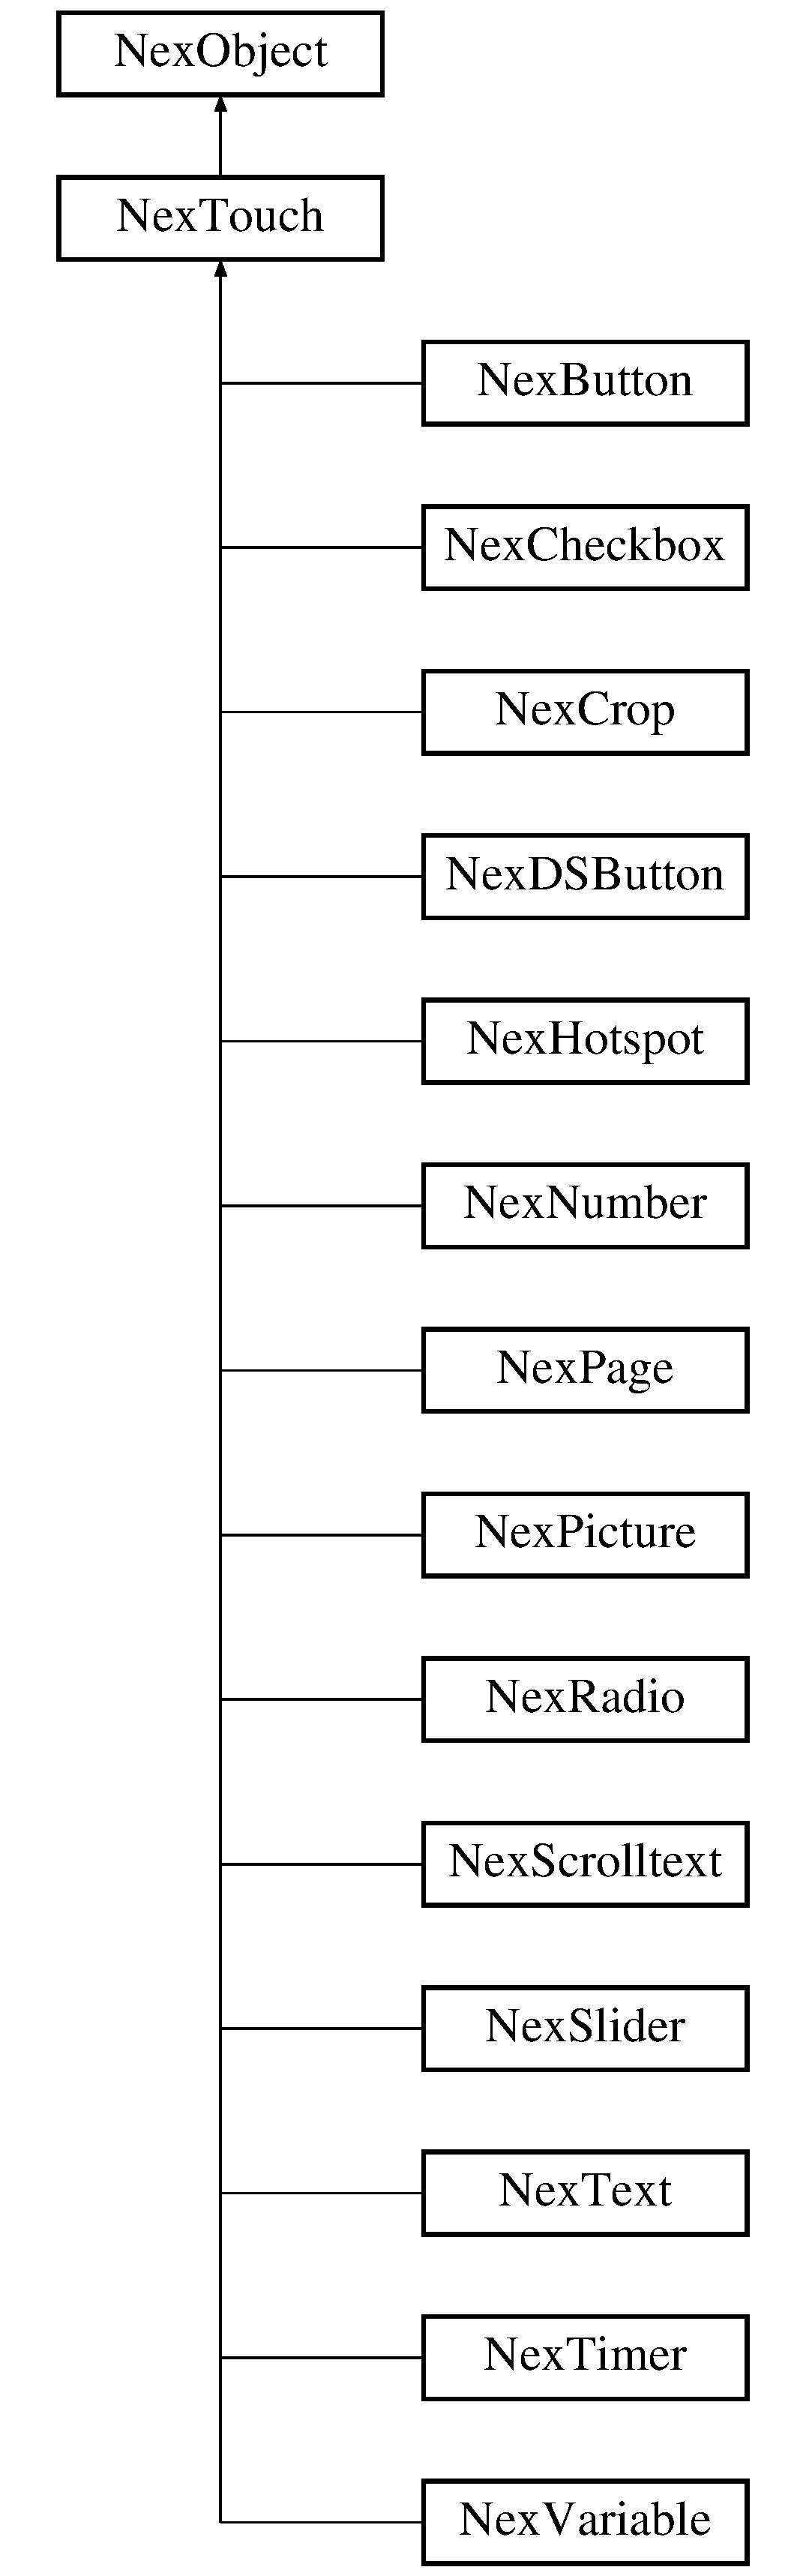
\includegraphics[height=12.000000cm]{class_nex_touch}
\end{center}
\end{figure}
\subsection*{Public Member Functions}
\begin{DoxyCompactItemize}
\item 
\hyperlink{class_nex_touch_a9e028e45e0d2d2cc39c8bf8d03dbb887}{Nex\+Touch} (uint8\+\_\+t pid, uint8\+\_\+t cid, const char $\ast$name)
\item 
void \hyperlink{class_nex_touch_a685a753aae5eb9fb9866a7807a310132}{attach\+Push} (\hyperlink{group___touch_event_ga162dea47b078e8878d10d6981a9dd0c6}{Nex\+Touch\+Event\+Cb} push, void $\ast$ptr=N\+U\+L\+L)
\item 
void \hyperlink{class_nex_touch_a2bc36096119534344c2bcd8021b93289}{detach\+Push} (void)
\item 
void \hyperlink{class_nex_touch_a4da1c4fcdfadb7eabfb9ccaba9ecad11}{attach\+Pop} (\hyperlink{group___touch_event_ga162dea47b078e8878d10d6981a9dd0c6}{Nex\+Touch\+Event\+Cb} pop, void $\ast$ptr=N\+U\+L\+L)
\item 
void \hyperlink{class_nex_touch_af656640c1078a553287a68bf792dd291}{detach\+Pop} (void)
\end{DoxyCompactItemize}
\subsection*{Static Public Member Functions}
\begin{DoxyCompactItemize}
\item 
\hypertarget{class_nex_touch_aa17cd9f742159ab61b60362b8d752b6f}{static void {\bfseries iterate} (\hyperlink{class_nex_touch}{Nex\+Touch} $\ast$$\ast$list, uint8\+\_\+t pid, uint8\+\_\+t cid, int32\+\_\+t event)}\label{class_nex_touch_aa17cd9f742159ab61b60362b8d752b6f}

\end{DoxyCompactItemize}
\subsection*{Additional Inherited Members}


\subsection{Detailed Description}
Father class of the components with touch events.

Derives from \hyperlink{class_nex_object}{Nex\+Object} and provides methods allowing user to attach (or detach) a callback function called when push(or pop) touch event occurs. 

\subsection{Constructor \& Destructor Documentation}
\hypertarget{class_nex_touch_a9e028e45e0d2d2cc39c8bf8d03dbb887}{\index{Nex\+Touch@{Nex\+Touch}!Nex\+Touch@{Nex\+Touch}}
\index{Nex\+Touch@{Nex\+Touch}!Nex\+Touch@{Nex\+Touch}}
\subsubsection[{Nex\+Touch}]{\setlength{\rightskip}{0pt plus 5cm}Nex\+Touch\+::\+Nex\+Touch (
\begin{DoxyParamCaption}
\item[{uint8\+\_\+t}]{pid, }
\item[{uint8\+\_\+t}]{cid, }
\item[{const char $\ast$}]{name}
\end{DoxyParamCaption}
)}}\label{class_nex_touch_a9e028e45e0d2d2cc39c8bf8d03dbb887}




Constructor.


\begin{DoxyParams}{Parameters}
{\em pid} & -\/ page id. \\
\hline
{\em cid} & -\/ component id. \\
\hline
{\em name} & -\/ pointer to an unique name in range of all components. \\
\hline
\end{DoxyParams}


\subsection{Member Function Documentation}
\hypertarget{class_nex_touch_a4da1c4fcdfadb7eabfb9ccaba9ecad11}{\index{Nex\+Touch@{Nex\+Touch}!attach\+Pop@{attach\+Pop}}
\index{attach\+Pop@{attach\+Pop}!Nex\+Touch@{Nex\+Touch}}
\subsubsection[{attach\+Pop}]{\setlength{\rightskip}{0pt plus 5cm}void Nex\+Touch\+::attach\+Pop (
\begin{DoxyParamCaption}
\item[{{\bf Nex\+Touch\+Event\+Cb}}]{pop, }
\item[{void $\ast$}]{ptr = {\ttfamily NULL}}
\end{DoxyParamCaption}
)}}\label{class_nex_touch_a4da1c4fcdfadb7eabfb9ccaba9ecad11}
Attach an callback function of pop touch event.


\begin{DoxyParams}{Parameters}
{\em pop} & -\/ callback called with ptr when a pop touch event occurs. \\
\hline
{\em ptr} & -\/ parameter passed into pop\mbox{[}default\+:N\+U\+L\+L\mbox{]}. \\
\hline
\end{DoxyParams}
\begin{DoxyReturn}{Returns}
none.
\end{DoxyReturn}
\begin{DoxyNote}{Note}
If calling this method multiply, the last call is valid. 
\end{DoxyNote}
\hypertarget{class_nex_touch_a685a753aae5eb9fb9866a7807a310132}{\index{Nex\+Touch@{Nex\+Touch}!attach\+Push@{attach\+Push}}
\index{attach\+Push@{attach\+Push}!Nex\+Touch@{Nex\+Touch}}
\subsubsection[{attach\+Push}]{\setlength{\rightskip}{0pt plus 5cm}void Nex\+Touch\+::attach\+Push (
\begin{DoxyParamCaption}
\item[{{\bf Nex\+Touch\+Event\+Cb}}]{push, }
\item[{void $\ast$}]{ptr = {\ttfamily NULL}}
\end{DoxyParamCaption}
)}}\label{class_nex_touch_a685a753aae5eb9fb9866a7807a310132}
Attach an callback function of push touch event.


\begin{DoxyParams}{Parameters}
{\em push} & -\/ callback called with ptr when a push touch event occurs. \\
\hline
{\em ptr} & -\/ parameter passed into push\mbox{[}default\+:N\+U\+L\+L\mbox{]}. \\
\hline
\end{DoxyParams}
\begin{DoxyReturn}{Returns}
none.
\end{DoxyReturn}
\begin{DoxyNote}{Note}
If calling this method multiply, the last call is valid. 
\end{DoxyNote}
\hypertarget{class_nex_touch_af656640c1078a553287a68bf792dd291}{\index{Nex\+Touch@{Nex\+Touch}!detach\+Pop@{detach\+Pop}}
\index{detach\+Pop@{detach\+Pop}!Nex\+Touch@{Nex\+Touch}}
\subsubsection[{detach\+Pop}]{\setlength{\rightskip}{0pt plus 5cm}void Nex\+Touch\+::detach\+Pop (
\begin{DoxyParamCaption}
\item[{void}]{}
\end{DoxyParamCaption}
)}}\label{class_nex_touch_af656640c1078a553287a68bf792dd291}
Detach an callback function.

\begin{DoxyReturn}{Returns}
none. 
\end{DoxyReturn}
\hypertarget{class_nex_touch_a2bc36096119534344c2bcd8021b93289}{\index{Nex\+Touch@{Nex\+Touch}!detach\+Push@{detach\+Push}}
\index{detach\+Push@{detach\+Push}!Nex\+Touch@{Nex\+Touch}}
\subsubsection[{detach\+Push}]{\setlength{\rightskip}{0pt plus 5cm}void Nex\+Touch\+::detach\+Push (
\begin{DoxyParamCaption}
\item[{void}]{}
\end{DoxyParamCaption}
)}}\label{class_nex_touch_a2bc36096119534344c2bcd8021b93289}
Detach an callback function.

\begin{DoxyReturn}{Returns}
none. 
\end{DoxyReturn}


The documentation for this class was generated from the following files\+:\begin{DoxyCompactItemize}
\item 
\hyperlink{_nex_touch_8h}{Nex\+Touch.\+h}\item 
\hyperlink{_nex_touch_8cpp}{Nex\+Touch.\+cpp}\end{DoxyCompactItemize}

\hypertarget{class_nex_upload}{\section{Nex\+Upload Class Reference}
\label{class_nex_upload}\index{Nex\+Upload@{Nex\+Upload}}
}


{\ttfamily \#include $<$Nex\+Upload.\+h$>$}

\subsection*{Public Member Functions}
\begin{DoxyCompactItemize}
\item 
\hyperlink{class_nex_upload_a017c25b02bc9a674ab5beb447a3511a0}{Nex\+Upload} (const char $\ast$file\+\_\+name, const uint8\+\_\+t S\+D\+\_\+chip\+\_\+select, uint32\+\_\+t download\+\_\+baudrate)
\item 
\hyperlink{class_nex_upload_a97d6aeee29cfdeb1ec4dcec8d5a58396}{Nex\+Upload} (const String file\+\_\+\+Name, const uint8\+\_\+t S\+D\+\_\+chip\+\_\+select, uint32\+\_\+t download\+\_\+baudrate)
\item 
\hyperlink{class_nex_upload_a26ccc2285435b6b573fa5c4b661c080a}{$\sim$\+Nex\+Upload} ()
\item 
\hypertarget{class_nex_upload_a42d3a6e05ba61b2590ea34687cfdb72a}{void {\bfseries upload} ()}\label{class_nex_upload_a42d3a6e05ba61b2590ea34687cfdb72a}

\end{DoxyCompactItemize}


\subsection{Detailed Description}
Provides the A\+P\+I for nextion to download the ftf file. 

\subsection{Constructor \& Destructor Documentation}
\hypertarget{class_nex_upload_a017c25b02bc9a674ab5beb447a3511a0}{\index{Nex\+Upload@{Nex\+Upload}!Nex\+Upload@{Nex\+Upload}}
\index{Nex\+Upload@{Nex\+Upload}!Nex\+Upload@{Nex\+Upload}}
\subsubsection[{Nex\+Upload}]{\setlength{\rightskip}{0pt plus 5cm}Nex\+Upload\+::\+Nex\+Upload (
\begin{DoxyParamCaption}
\item[{const char $\ast$}]{file\+\_\+name, }
\item[{const uint8\+\_\+t}]{S\+D\+\_\+chip\+\_\+select, }
\item[{uint32\+\_\+t}]{download\+\_\+baudrate}
\end{DoxyParamCaption}
)}}\label{class_nex_upload_a017c25b02bc9a674ab5beb447a3511a0}
Constructor.


\begin{DoxyParams}{Parameters}
{\em file\+\_\+name} & -\/ tft file name. \\
\hline
{\em S\+D\+\_\+chip\+\_\+select} & -\/ sd chip select pin. \\
\hline
{\em download\+\_\+baudrate} & -\/ set download baudrate. \\
\hline
\end{DoxyParams}
\hypertarget{class_nex_upload_a97d6aeee29cfdeb1ec4dcec8d5a58396}{\index{Nex\+Upload@{Nex\+Upload}!Nex\+Upload@{Nex\+Upload}}
\index{Nex\+Upload@{Nex\+Upload}!Nex\+Upload@{Nex\+Upload}}
\subsubsection[{Nex\+Upload}]{\setlength{\rightskip}{0pt plus 5cm}Nex\+Upload\+::\+Nex\+Upload (
\begin{DoxyParamCaption}
\item[{const String}]{file\+\_\+\+Name, }
\item[{const uint8\+\_\+t}]{S\+D\+\_\+chip\+\_\+select, }
\item[{uint32\+\_\+t}]{download\+\_\+baudrate}
\end{DoxyParamCaption}
)}}\label{class_nex_upload_a97d6aeee29cfdeb1ec4dcec8d5a58396}
Constructor.


\begin{DoxyParams}{Parameters}
{\em file\+\_\+\+Name} & -\/ tft file name. \\
\hline
{\em S\+D\+\_\+chip\+\_\+select} & -\/ sd chip select pin. \\
\hline
{\em download\+\_\+baudrate} & -\/ set download baudrate. \\
\hline
\end{DoxyParams}
\hypertarget{class_nex_upload_a26ccc2285435b6b573fa5c4b661c080a}{\index{Nex\+Upload@{Nex\+Upload}!````~Nex\+Upload@{$\sim$\+Nex\+Upload}}
\index{````~Nex\+Upload@{$\sim$\+Nex\+Upload}!Nex\+Upload@{Nex\+Upload}}
\subsubsection[{$\sim$\+Nex\+Upload}]{\setlength{\rightskip}{0pt plus 5cm}Nex\+Upload\+::$\sim$\+Nex\+Upload (
\begin{DoxyParamCaption}
{}
\end{DoxyParamCaption}
)\hspace{0.3cm}{\ttfamily [inline]}}}\label{class_nex_upload_a26ccc2285435b6b573fa5c4b661c080a}
destructor. 

The documentation for this class was generated from the following files\+:\begin{DoxyCompactItemize}
\item 
\hyperlink{_nex_upload_8h}{Nex\+Upload.\+h}\item 
\hyperlink{_nex_upload_8cpp}{Nex\+Upload.\+cpp}\end{DoxyCompactItemize}

\hypertarget{class_nex_variable}{\section{Nex\+Variable Class Reference}
\label{class_nex_variable}\index{Nex\+Variable@{Nex\+Variable}}
}


{\ttfamily \#include $<$Nex\+Variable.\+h$>$}

Inheritance diagram for Nex\+Variable\+:\begin{figure}[H]
\begin{center}
\leavevmode
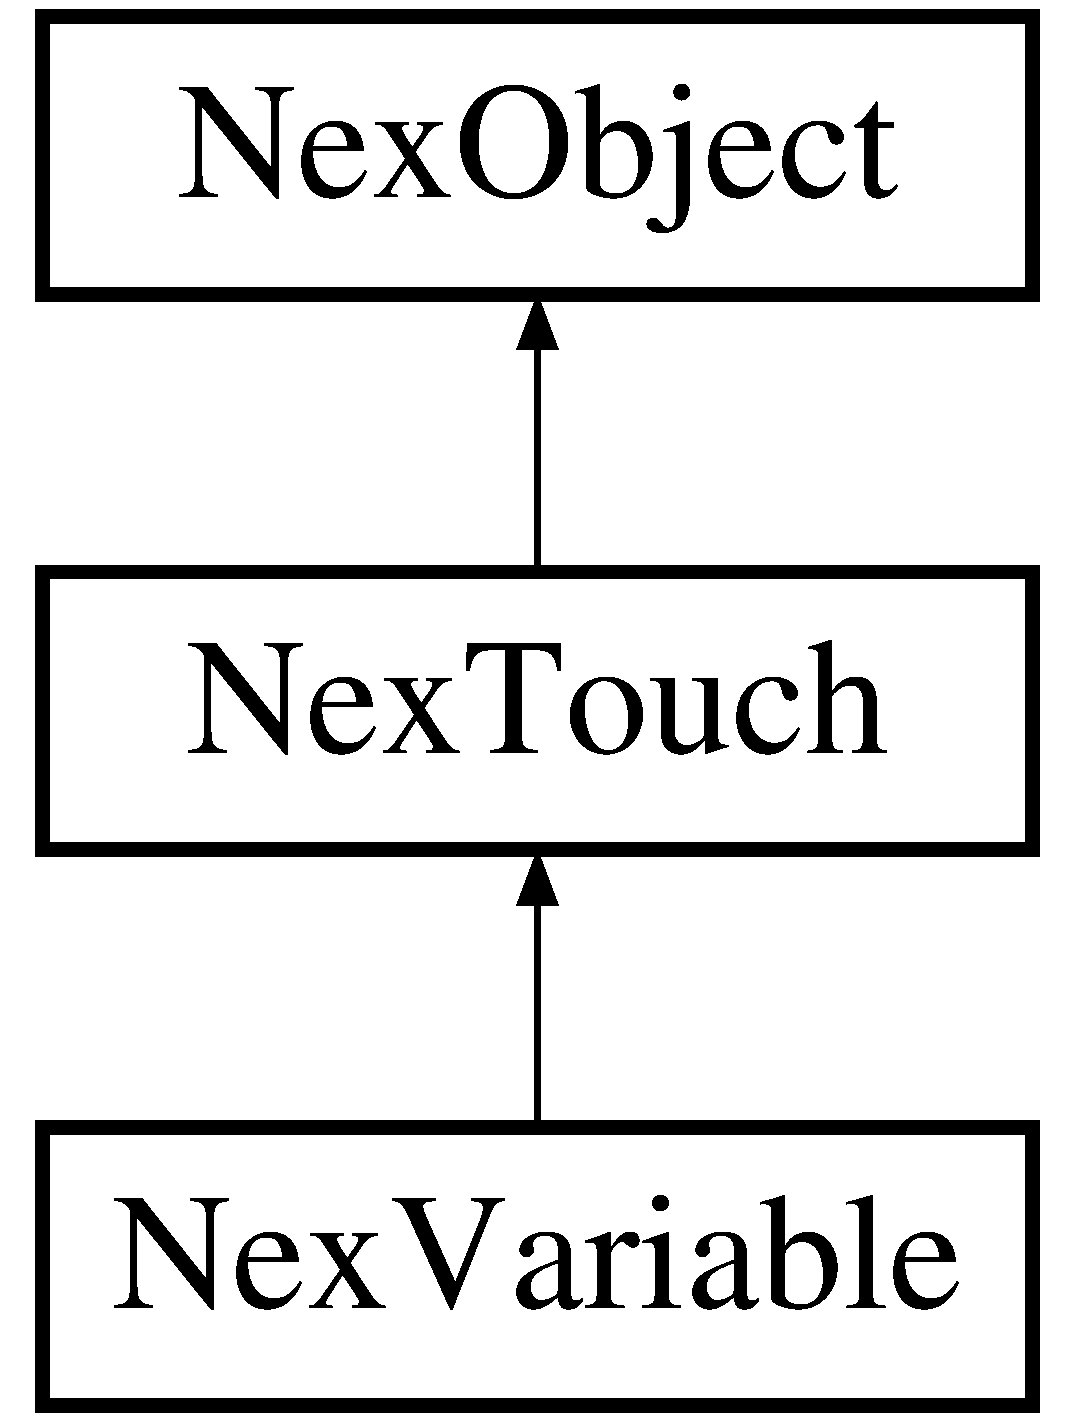
\includegraphics[height=3.000000cm]{class_nex_variable}
\end{center}
\end{figure}
\subsection*{Public Member Functions}
\begin{DoxyCompactItemize}
\item 
\hyperlink{class_nex_variable_a7d36d19e14c991872fb1547f3ced09b2}{Nex\+Variable} (uint8\+\_\+t pid, uint8\+\_\+t cid, const char $\ast$name)
\item 
uint32\+\_\+t \hyperlink{class_nex_variable_ab4d12f14dcff3f6930a2bdf5e1f3d259}{get\+Text} (char $\ast$buffer, uint32\+\_\+t len)
\item 
bool \hyperlink{class_nex_variable_aab59ac44eb0804664a03c09932be70eb}{set\+Text} (const char $\ast$buffer)
\item 
uint32\+\_\+t \hyperlink{class_nex_variable_aff06d16d022876c749d3e30f020b1557}{get\+Value} (uint32\+\_\+t $\ast$number)
\item 
bool \hyperlink{class_nex_variable_a9da9d4a74f09e1787e4e4562da1e4833}{set\+Value} (uint32\+\_\+t number)
\end{DoxyCompactItemize}
\subsection*{Additional Inherited Members}


\subsection{Detailed Description}
\hyperlink{class_nex_button}{Nex\+Button} component.

Commonly, you want to do something after push and pop it. It is recommanded that only call \hyperlink{class_nex_touch_a4da1c4fcdfadb7eabfb9ccaba9ecad11}{Nex\+Touch\+::attach\+Pop} to satisfy your purpose.

\begin{DoxyWarning}{Warning}
Please do not call \hyperlink{class_nex_touch_a685a753aae5eb9fb9866a7807a310132}{Nex\+Touch\+::attach\+Push} on this component, even though you can. 
\end{DoxyWarning}


\subsection{Constructor \& Destructor Documentation}
\hypertarget{class_nex_variable_a7d36d19e14c991872fb1547f3ced09b2}{\index{Nex\+Variable@{Nex\+Variable}!Nex\+Variable@{Nex\+Variable}}
\index{Nex\+Variable@{Nex\+Variable}!Nex\+Variable@{Nex\+Variable}}
\subsubsection[{Nex\+Variable}]{\setlength{\rightskip}{0pt plus 5cm}Nex\+Variable\+::\+Nex\+Variable (
\begin{DoxyParamCaption}
\item[{uint8\+\_\+t}]{pid, }
\item[{uint8\+\_\+t}]{cid, }
\item[{const char $\ast$}]{name}
\end{DoxyParamCaption}
)}}\label{class_nex_variable_a7d36d19e14c991872fb1547f3ced09b2}




Constructor.


\begin{DoxyParams}{Parameters}
{\em pid} & -\/ page id. \\
\hline
{\em cid} & -\/ component id. \\
\hline
{\em name} & -\/ pointer to an unique name in range of all components. \\
\hline
\end{DoxyParams}


\subsection{Member Function Documentation}
\hypertarget{class_nex_variable_ab4d12f14dcff3f6930a2bdf5e1f3d259}{\index{Nex\+Variable@{Nex\+Variable}!get\+Text@{get\+Text}}
\index{get\+Text@{get\+Text}!Nex\+Variable@{Nex\+Variable}}
\subsubsection[{get\+Text}]{\setlength{\rightskip}{0pt plus 5cm}uint32\+\_\+t Nex\+Variable\+::get\+Text (
\begin{DoxyParamCaption}
\item[{char $\ast$}]{buffer, }
\item[{uint32\+\_\+t}]{len}
\end{DoxyParamCaption}
)}}\label{class_nex_variable_ab4d12f14dcff3f6930a2bdf5e1f3d259}
Get text attribute of component.


\begin{DoxyParams}{Parameters}
{\em buffer} & -\/ buffer storing text returned. \\
\hline
{\em len} & -\/ length of buffer. \\
\hline
\end{DoxyParams}
\begin{DoxyReturn}{Returns}
The real length of text returned. 
\end{DoxyReturn}
\hypertarget{class_nex_variable_aff06d16d022876c749d3e30f020b1557}{\index{Nex\+Variable@{Nex\+Variable}!get\+Value@{get\+Value}}
\index{get\+Value@{get\+Value}!Nex\+Variable@{Nex\+Variable}}
\subsubsection[{get\+Value}]{\setlength{\rightskip}{0pt plus 5cm}uint32\+\_\+t Nex\+Variable\+::get\+Value (
\begin{DoxyParamCaption}
\item[{uint32\+\_\+t $\ast$}]{number}
\end{DoxyParamCaption}
)}}\label{class_nex_variable_aff06d16d022876c749d3e30f020b1557}
Get val attribute of component


\begin{DoxyParams}{Parameters}
{\em number} & -\/ buffer storing data retur \\
\hline
\end{DoxyParams}
\begin{DoxyReturn}{Returns}
the length of the data 
\end{DoxyReturn}
\hypertarget{class_nex_variable_aab59ac44eb0804664a03c09932be70eb}{\index{Nex\+Variable@{Nex\+Variable}!set\+Text@{set\+Text}}
\index{set\+Text@{set\+Text}!Nex\+Variable@{Nex\+Variable}}
\subsubsection[{set\+Text}]{\setlength{\rightskip}{0pt plus 5cm}bool Nex\+Variable\+::set\+Text (
\begin{DoxyParamCaption}
\item[{const char $\ast$}]{buffer}
\end{DoxyParamCaption}
)}}\label{class_nex_variable_aab59ac44eb0804664a03c09932be70eb}
Set text attribute of component.


\begin{DoxyParams}{Parameters}
{\em buffer} & -\/ text buffer terminated with '\textbackslash{}0'. \\
\hline
\end{DoxyParams}
\begin{DoxyReturn}{Returns}
true if success, false for failure. 
\end{DoxyReturn}
\hypertarget{class_nex_variable_a9da9d4a74f09e1787e4e4562da1e4833}{\index{Nex\+Variable@{Nex\+Variable}!set\+Value@{set\+Value}}
\index{set\+Value@{set\+Value}!Nex\+Variable@{Nex\+Variable}}
\subsubsection[{set\+Value}]{\setlength{\rightskip}{0pt plus 5cm}bool Nex\+Variable\+::set\+Value (
\begin{DoxyParamCaption}
\item[{uint32\+\_\+t}]{number}
\end{DoxyParamCaption}
)}}\label{class_nex_variable_a9da9d4a74f09e1787e4e4562da1e4833}
Set val attribute of component


\begin{DoxyParams}{Parameters}
{\em number} & -\/ To set up the data \\
\hline
\end{DoxyParams}
\begin{DoxyReturn}{Returns}
true if success, false for failure 
\end{DoxyReturn}


The documentation for this class was generated from the following files\+:\begin{DoxyCompactItemize}
\item 
Nex\+Variable.\+h\item 
\hyperlink{_nex_variable_8cpp}{Nex\+Variable.\+cpp}\end{DoxyCompactItemize}

\hypertarget{class_nex_waveform}{\section{Nex\+Waveform Class Reference}
\label{class_nex_waveform}\index{Nex\+Waveform@{Nex\+Waveform}}
}


{\ttfamily \#include $<$Nex\+Waveform.\+h$>$}

Inheritance diagram for Nex\+Waveform\+:\begin{figure}[H]
\begin{center}
\leavevmode
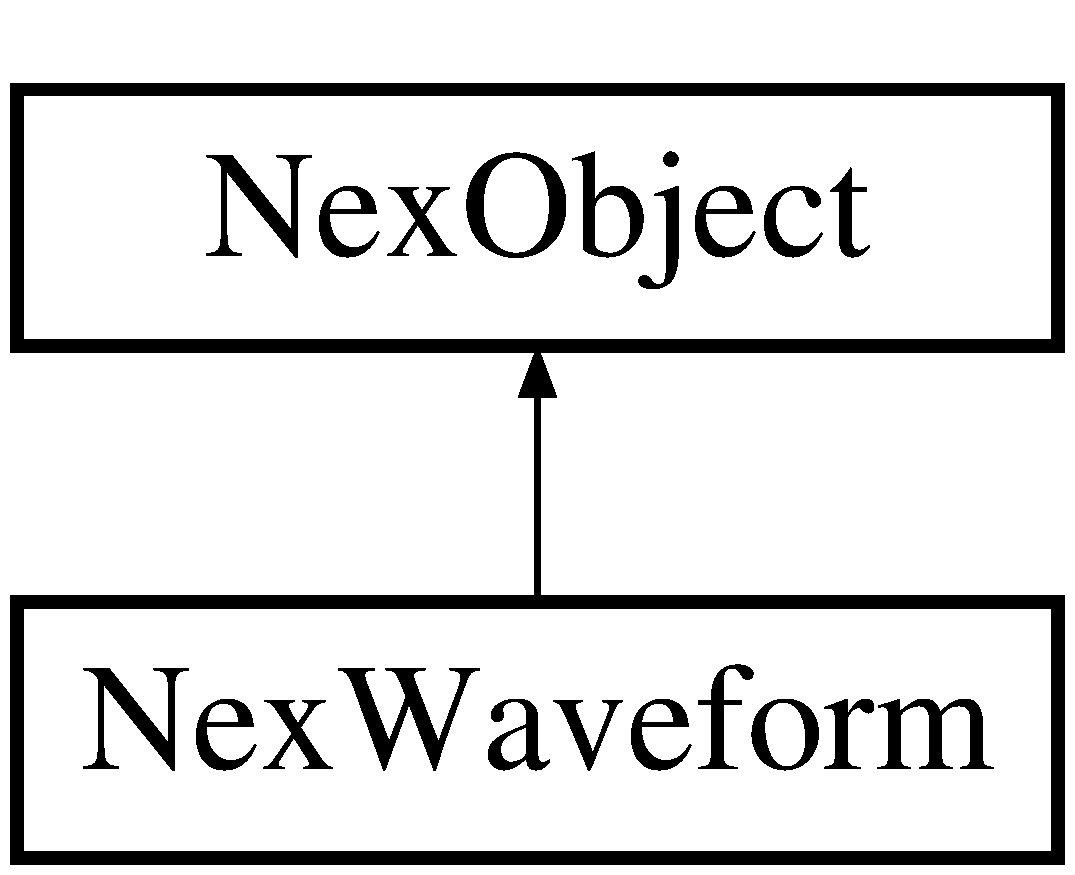
\includegraphics[height=2.000000cm]{class_nex_waveform}
\end{center}
\end{figure}
\subsection*{Public Member Functions}
\begin{DoxyCompactItemize}
\item 
\hyperlink{class_nex_waveform_a4f18ca5050823e874d526141c8595514}{Nex\+Waveform} (uint8\+\_\+t pid, uint8\+\_\+t cid, const char $\ast$name)
\item 
bool \hyperlink{class_nex_waveform_a5b04ea7397b784947b845e2a03fc77e4}{add\+Value} (uint8\+\_\+t ch, uint8\+\_\+t number)
\item 
uint32\+\_\+t \hyperlink{class_nex_waveform_a66cec3c4d0d1a769dbf50c8092cc01d1}{Get\+\_\+background\+\_\+color\+\_\+bco} (uint32\+\_\+t $\ast$number)
\item 
bool \hyperlink{class_nex_waveform_aefec5eb25ee698c8c940c9190d60b696}{Set\+\_\+background\+\_\+color\+\_\+bco} (uint32\+\_\+t number)
\item 
uint32\+\_\+t \hyperlink{class_nex_waveform_ac5a6622e9004600f24b12e60ebb6b984}{Get\+\_\+grid\+\_\+color\+\_\+gdc} (uint32\+\_\+t $\ast$number)
\item 
bool \hyperlink{class_nex_waveform_ab396211f736824a0210446e68dc3edf4}{Set\+\_\+grid\+\_\+color\+\_\+gdc} (uint32\+\_\+t number)
\item 
uint32\+\_\+t \hyperlink{class_nex_waveform_ad5c4968c81d4941a08841cbaf217c631}{Get\+\_\+grid\+\_\+width\+\_\+gdw} (uint32\+\_\+t $\ast$number)
\item 
bool \hyperlink{class_nex_waveform_a41cb6d8b1ff6c309d1c4e8a1f73304fe}{Set\+\_\+grid\+\_\+width\+\_\+gdw} (uint32\+\_\+t number)
\item 
uint32\+\_\+t \hyperlink{class_nex_waveform_a87f6baf5a7a9c52f54281865e757d9a3}{Get\+\_\+grid\+\_\+height\+\_\+gdh} (uint32\+\_\+t $\ast$number)
\item 
bool \hyperlink{class_nex_waveform_a85e776a5347c22efd9abe9bb8cfdbddb}{Set\+\_\+grid\+\_\+height\+\_\+gdh} (uint32\+\_\+t number)
\item 
uint32\+\_\+t \hyperlink{class_nex_waveform_a09e36144f65c73b21edcfd5caff8a914}{Get\+\_\+channel\+\_\+0\+\_\+color\+\_\+pco0} (uint32\+\_\+t $\ast$number)
\item 
bool \hyperlink{class_nex_waveform_ade323e0eae3b5058a76245e5ac97b037}{Set\+\_\+channel\+\_\+0\+\_\+color\+\_\+pco0} (uint32\+\_\+t number)
\end{DoxyCompactItemize}
\subsection*{Additional Inherited Members}


\subsection{Detailed Description}
\hyperlink{class_nex_waveform}{Nex\+Waveform} component. 

\subsection{Constructor \& Destructor Documentation}
\hypertarget{class_nex_waveform_a4f18ca5050823e874d526141c8595514}{\index{Nex\+Waveform@{Nex\+Waveform}!Nex\+Waveform@{Nex\+Waveform}}
\index{Nex\+Waveform@{Nex\+Waveform}!Nex\+Waveform@{Nex\+Waveform}}
\subsubsection[{Nex\+Waveform}]{\setlength{\rightskip}{0pt plus 5cm}Nex\+Waveform\+::\+Nex\+Waveform (
\begin{DoxyParamCaption}
\item[{uint8\+\_\+t}]{pid, }
\item[{uint8\+\_\+t}]{cid, }
\item[{const char $\ast$}]{name}
\end{DoxyParamCaption}
)}}\label{class_nex_waveform_a4f18ca5050823e874d526141c8595514}




Constructor.


\begin{DoxyParams}{Parameters}
{\em pid} & -\/ page id. \\
\hline
{\em cid} & -\/ component id. \\
\hline
{\em name} & -\/ pointer to an unique name in range of all components. \\
\hline
\end{DoxyParams}


\subsection{Member Function Documentation}
\hypertarget{class_nex_waveform_a5b04ea7397b784947b845e2a03fc77e4}{\index{Nex\+Waveform@{Nex\+Waveform}!add\+Value@{add\+Value}}
\index{add\+Value@{add\+Value}!Nex\+Waveform@{Nex\+Waveform}}
\subsubsection[{add\+Value}]{\setlength{\rightskip}{0pt plus 5cm}bool Nex\+Waveform\+::add\+Value (
\begin{DoxyParamCaption}
\item[{uint8\+\_\+t}]{ch, }
\item[{uint8\+\_\+t}]{number}
\end{DoxyParamCaption}
)}}\label{class_nex_waveform_a5b04ea7397b784947b845e2a03fc77e4}
Add value to show.


\begin{DoxyParams}{Parameters}
{\em ch} & -\/ channel of waveform(0-\/3). \\
\hline
{\em number} & -\/ the value of waveform.\\
\hline
\end{DoxyParams}

\begin{DoxyRetVals}{Return values}
{\em true} & -\/ success. \\
\hline
{\em false} & -\/ failed. \\
\hline
\end{DoxyRetVals}
\hypertarget{class_nex_waveform_a66cec3c4d0d1a769dbf50c8092cc01d1}{\index{Nex\+Waveform@{Nex\+Waveform}!Get\+\_\+background\+\_\+color\+\_\+bco@{Get\+\_\+background\+\_\+color\+\_\+bco}}
\index{Get\+\_\+background\+\_\+color\+\_\+bco@{Get\+\_\+background\+\_\+color\+\_\+bco}!Nex\+Waveform@{Nex\+Waveform}}
\subsubsection[{Get\+\_\+background\+\_\+color\+\_\+bco}]{\setlength{\rightskip}{0pt plus 5cm}uint32\+\_\+t Nex\+Waveform\+::\+Get\+\_\+background\+\_\+color\+\_\+bco (
\begin{DoxyParamCaption}
\item[{uint32\+\_\+t $\ast$}]{number}
\end{DoxyParamCaption}
)}}\label{class_nex_waveform_a66cec3c4d0d1a769dbf50c8092cc01d1}
Get bco attribute of component


\begin{DoxyParams}{Parameters}
{\em number} & -\/ buffer storing data retur \\
\hline
\end{DoxyParams}
\begin{DoxyReturn}{Returns}
the length of the data 
\end{DoxyReturn}
\hypertarget{class_nex_waveform_a09e36144f65c73b21edcfd5caff8a914}{\index{Nex\+Waveform@{Nex\+Waveform}!Get\+\_\+channel\+\_\+0\+\_\+color\+\_\+pco0@{Get\+\_\+channel\+\_\+0\+\_\+color\+\_\+pco0}}
\index{Get\+\_\+channel\+\_\+0\+\_\+color\+\_\+pco0@{Get\+\_\+channel\+\_\+0\+\_\+color\+\_\+pco0}!Nex\+Waveform@{Nex\+Waveform}}
\subsubsection[{Get\+\_\+channel\+\_\+0\+\_\+color\+\_\+pco0}]{\setlength{\rightskip}{0pt plus 5cm}uint32\+\_\+t Nex\+Waveform\+::\+Get\+\_\+channel\+\_\+0\+\_\+color\+\_\+pco0 (
\begin{DoxyParamCaption}
\item[{uint32\+\_\+t $\ast$}]{number}
\end{DoxyParamCaption}
)}}\label{class_nex_waveform_a09e36144f65c73b21edcfd5caff8a914}
Get pco0 attribute of component


\begin{DoxyParams}{Parameters}
{\em number} & -\/ buffer storing data retur \\
\hline
\end{DoxyParams}
\begin{DoxyReturn}{Returns}
the length of the data 
\end{DoxyReturn}
\hypertarget{class_nex_waveform_ac5a6622e9004600f24b12e60ebb6b984}{\index{Nex\+Waveform@{Nex\+Waveform}!Get\+\_\+grid\+\_\+color\+\_\+gdc@{Get\+\_\+grid\+\_\+color\+\_\+gdc}}
\index{Get\+\_\+grid\+\_\+color\+\_\+gdc@{Get\+\_\+grid\+\_\+color\+\_\+gdc}!Nex\+Waveform@{Nex\+Waveform}}
\subsubsection[{Get\+\_\+grid\+\_\+color\+\_\+gdc}]{\setlength{\rightskip}{0pt plus 5cm}uint32\+\_\+t Nex\+Waveform\+::\+Get\+\_\+grid\+\_\+color\+\_\+gdc (
\begin{DoxyParamCaption}
\item[{uint32\+\_\+t $\ast$}]{number}
\end{DoxyParamCaption}
)}}\label{class_nex_waveform_ac5a6622e9004600f24b12e60ebb6b984}
Get gdc attribute of component


\begin{DoxyParams}{Parameters}
{\em number} & -\/ buffer storing data retur \\
\hline
\end{DoxyParams}
\begin{DoxyReturn}{Returns}
the length of the data 
\end{DoxyReturn}
\hypertarget{class_nex_waveform_a87f6baf5a7a9c52f54281865e757d9a3}{\index{Nex\+Waveform@{Nex\+Waveform}!Get\+\_\+grid\+\_\+height\+\_\+gdh@{Get\+\_\+grid\+\_\+height\+\_\+gdh}}
\index{Get\+\_\+grid\+\_\+height\+\_\+gdh@{Get\+\_\+grid\+\_\+height\+\_\+gdh}!Nex\+Waveform@{Nex\+Waveform}}
\subsubsection[{Get\+\_\+grid\+\_\+height\+\_\+gdh}]{\setlength{\rightskip}{0pt plus 5cm}uint32\+\_\+t Nex\+Waveform\+::\+Get\+\_\+grid\+\_\+height\+\_\+gdh (
\begin{DoxyParamCaption}
\item[{uint32\+\_\+t $\ast$}]{number}
\end{DoxyParamCaption}
)}}\label{class_nex_waveform_a87f6baf5a7a9c52f54281865e757d9a3}
Get gdh attribute of component


\begin{DoxyParams}{Parameters}
{\em number} & -\/ buffer storing data retur \\
\hline
\end{DoxyParams}
\begin{DoxyReturn}{Returns}
the length of the data 
\end{DoxyReturn}
\hypertarget{class_nex_waveform_ad5c4968c81d4941a08841cbaf217c631}{\index{Nex\+Waveform@{Nex\+Waveform}!Get\+\_\+grid\+\_\+width\+\_\+gdw@{Get\+\_\+grid\+\_\+width\+\_\+gdw}}
\index{Get\+\_\+grid\+\_\+width\+\_\+gdw@{Get\+\_\+grid\+\_\+width\+\_\+gdw}!Nex\+Waveform@{Nex\+Waveform}}
\subsubsection[{Get\+\_\+grid\+\_\+width\+\_\+gdw}]{\setlength{\rightskip}{0pt plus 5cm}uint32\+\_\+t Nex\+Waveform\+::\+Get\+\_\+grid\+\_\+width\+\_\+gdw (
\begin{DoxyParamCaption}
\item[{uint32\+\_\+t $\ast$}]{number}
\end{DoxyParamCaption}
)}}\label{class_nex_waveform_ad5c4968c81d4941a08841cbaf217c631}
Get gdw attribute of component


\begin{DoxyParams}{Parameters}
{\em number} & -\/ buffer storing data retur \\
\hline
\end{DoxyParams}
\begin{DoxyReturn}{Returns}
the length of the data 
\end{DoxyReturn}
\hypertarget{class_nex_waveform_aefec5eb25ee698c8c940c9190d60b696}{\index{Nex\+Waveform@{Nex\+Waveform}!Set\+\_\+background\+\_\+color\+\_\+bco@{Set\+\_\+background\+\_\+color\+\_\+bco}}
\index{Set\+\_\+background\+\_\+color\+\_\+bco@{Set\+\_\+background\+\_\+color\+\_\+bco}!Nex\+Waveform@{Nex\+Waveform}}
\subsubsection[{Set\+\_\+background\+\_\+color\+\_\+bco}]{\setlength{\rightskip}{0pt plus 5cm}bool Nex\+Waveform\+::\+Set\+\_\+background\+\_\+color\+\_\+bco (
\begin{DoxyParamCaption}
\item[{uint32\+\_\+t}]{number}
\end{DoxyParamCaption}
)}}\label{class_nex_waveform_aefec5eb25ee698c8c940c9190d60b696}
Set bco attribute of component


\begin{DoxyParams}{Parameters}
{\em number} & -\/ To set up the data \\
\hline
\end{DoxyParams}
\begin{DoxyReturn}{Returns}
true if success, false for failure 
\end{DoxyReturn}
\hypertarget{class_nex_waveform_ade323e0eae3b5058a76245e5ac97b037}{\index{Nex\+Waveform@{Nex\+Waveform}!Set\+\_\+channel\+\_\+0\+\_\+color\+\_\+pco0@{Set\+\_\+channel\+\_\+0\+\_\+color\+\_\+pco0}}
\index{Set\+\_\+channel\+\_\+0\+\_\+color\+\_\+pco0@{Set\+\_\+channel\+\_\+0\+\_\+color\+\_\+pco0}!Nex\+Waveform@{Nex\+Waveform}}
\subsubsection[{Set\+\_\+channel\+\_\+0\+\_\+color\+\_\+pco0}]{\setlength{\rightskip}{0pt plus 5cm}bool Nex\+Waveform\+::\+Set\+\_\+channel\+\_\+0\+\_\+color\+\_\+pco0 (
\begin{DoxyParamCaption}
\item[{uint32\+\_\+t}]{number}
\end{DoxyParamCaption}
)}}\label{class_nex_waveform_ade323e0eae3b5058a76245e5ac97b037}
Set pco0 attribute of component


\begin{DoxyParams}{Parameters}
{\em number} & -\/ To set up the data \\
\hline
\end{DoxyParams}
\begin{DoxyReturn}{Returns}
true if success, false for failure 
\end{DoxyReturn}
\hypertarget{class_nex_waveform_ab396211f736824a0210446e68dc3edf4}{\index{Nex\+Waveform@{Nex\+Waveform}!Set\+\_\+grid\+\_\+color\+\_\+gdc@{Set\+\_\+grid\+\_\+color\+\_\+gdc}}
\index{Set\+\_\+grid\+\_\+color\+\_\+gdc@{Set\+\_\+grid\+\_\+color\+\_\+gdc}!Nex\+Waveform@{Nex\+Waveform}}
\subsubsection[{Set\+\_\+grid\+\_\+color\+\_\+gdc}]{\setlength{\rightskip}{0pt plus 5cm}bool Nex\+Waveform\+::\+Set\+\_\+grid\+\_\+color\+\_\+gdc (
\begin{DoxyParamCaption}
\item[{uint32\+\_\+t}]{number}
\end{DoxyParamCaption}
)}}\label{class_nex_waveform_ab396211f736824a0210446e68dc3edf4}
Set gdc attribute of component


\begin{DoxyParams}{Parameters}
{\em number} & -\/ To set up the data \\
\hline
\end{DoxyParams}
\begin{DoxyReturn}{Returns}
true if success, false for failure 
\end{DoxyReturn}
\hypertarget{class_nex_waveform_a85e776a5347c22efd9abe9bb8cfdbddb}{\index{Nex\+Waveform@{Nex\+Waveform}!Set\+\_\+grid\+\_\+height\+\_\+gdh@{Set\+\_\+grid\+\_\+height\+\_\+gdh}}
\index{Set\+\_\+grid\+\_\+height\+\_\+gdh@{Set\+\_\+grid\+\_\+height\+\_\+gdh}!Nex\+Waveform@{Nex\+Waveform}}
\subsubsection[{Set\+\_\+grid\+\_\+height\+\_\+gdh}]{\setlength{\rightskip}{0pt plus 5cm}bool Nex\+Waveform\+::\+Set\+\_\+grid\+\_\+height\+\_\+gdh (
\begin{DoxyParamCaption}
\item[{uint32\+\_\+t}]{number}
\end{DoxyParamCaption}
)}}\label{class_nex_waveform_a85e776a5347c22efd9abe9bb8cfdbddb}
Set gdh attribute of component


\begin{DoxyParams}{Parameters}
{\em number} & -\/ To set up the data \\
\hline
\end{DoxyParams}
\begin{DoxyReturn}{Returns}
true if success, false for failure 
\end{DoxyReturn}
\hypertarget{class_nex_waveform_a41cb6d8b1ff6c309d1c4e8a1f73304fe}{\index{Nex\+Waveform@{Nex\+Waveform}!Set\+\_\+grid\+\_\+width\+\_\+gdw@{Set\+\_\+grid\+\_\+width\+\_\+gdw}}
\index{Set\+\_\+grid\+\_\+width\+\_\+gdw@{Set\+\_\+grid\+\_\+width\+\_\+gdw}!Nex\+Waveform@{Nex\+Waveform}}
\subsubsection[{Set\+\_\+grid\+\_\+width\+\_\+gdw}]{\setlength{\rightskip}{0pt plus 5cm}bool Nex\+Waveform\+::\+Set\+\_\+grid\+\_\+width\+\_\+gdw (
\begin{DoxyParamCaption}
\item[{uint32\+\_\+t}]{number}
\end{DoxyParamCaption}
)}}\label{class_nex_waveform_a41cb6d8b1ff6c309d1c4e8a1f73304fe}
Set gdw attribute of component


\begin{DoxyParams}{Parameters}
{\em number} & -\/ To set up the data \\
\hline
\end{DoxyParams}
\begin{DoxyReturn}{Returns}
true if success, false for failure 
\end{DoxyReturn}


The documentation for this class was generated from the following files\+:\begin{DoxyCompactItemize}
\item 
\hyperlink{_nex_waveform_8h}{Nex\+Waveform.\+h}\item 
\hyperlink{_nex_waveform_8cpp}{Nex\+Waveform.\+cpp}\end{DoxyCompactItemize}

\chapter{File Documentation}
\hypertarget{doxygen_8h}{\section{doxygen.\+h File Reference}
\label{doxygen_8h}\index{doxygen.\+h@{doxygen.\+h}}
}


\subsection{Detailed Description}
Define modules in A\+P\+I doc.

\begin{DoxyAuthor}{Author}
Wu Pengfei (email\+:\href{mailto:pengfei.wu@itead.cc}{\tt pengfei.\+wu@itead.\+cc}) 
\end{DoxyAuthor}
\begin{DoxyDate}{Date}
2015/8/12 
\end{DoxyDate}
\begin{DoxyCopyright}{Copyright}
Copyright (C) 2013-\/2014 I\+T\+E\+A\+D Intelligent Systems Co., Ltd. ~\newline
This program is free software; you can redistribute it and/or modify it under the terms of the G\+N\+U General Public License as published by the Free Software Foundation; either version 2 of the License, or (at your option) any later version. 
\end{DoxyCopyright}

\hypertarget{_nex_button_8cpp}{\section{Nex\+Button.\+cpp File Reference}
\label{_nex_button_8cpp}\index{Nex\+Button.\+cpp@{Nex\+Button.\+cpp}}
}
{\ttfamily \#include \char`\"{}Nex\+Button.\+h\char`\"{}}\\*


\subsection{Detailed Description}
The implementation of class \hyperlink{class_nex_button}{Nex\+Button}.

\begin{DoxyAuthor}{Author}
Wu Pengfei (email\+:\href{mailto:pengfei.wu@itead.cc}{\tt pengfei.\+wu@itead.\+cc}) 
\end{DoxyAuthor}
\begin{DoxyDate}{Date}
2015/8/13 
\end{DoxyDate}
\begin{DoxyCopyright}{Copyright}
Copyright (C) 2014-\/2015 I\+T\+E\+A\+D Intelligent Systems Co., Ltd. ~\newline
This program is free software; you can redistribute it and/or modify it under the terms of the G\+N\+U General Public License as published by the Free Software Foundation; either version 2 of the License, or (at your option) any later version. 
\end{DoxyCopyright}

\hypertarget{_nex_button_8h}{\section{Nex\+Button.\+h File Reference}
\label{_nex_button_8h}\index{Nex\+Button.\+h@{Nex\+Button.\+h}}
}
{\ttfamily \#include \char`\"{}Nex\+Touch.\+h\char`\"{}}\\*
{\ttfamily \#include \char`\"{}Nex\+Hardware.\+h\char`\"{}}\\*
\subsection*{Classes}
\begin{DoxyCompactItemize}
\item 
class \hyperlink{class_nex_button}{Nex\+Button}
\end{DoxyCompactItemize}


\subsection{Detailed Description}
The definition of class \hyperlink{class_nex_button}{Nex\+Button}.

\begin{DoxyAuthor}{Author}
Wu Pengfei (email\+:\href{mailto:pengfei.wu@itead.cc}{\tt pengfei.\+wu@itead.\+cc}) 
\end{DoxyAuthor}
\begin{DoxyDate}{Date}
2015/8/13
\end{DoxyDate}
\begin{DoxyCopyright}{Copyright}
Copyright (C) 2014-\/2015 I\+T\+E\+A\+D Intelligent Systems Co., Ltd. ~\newline
This program is free software; you can redistribute it and/or modify it under the terms of the G\+N\+U General Public License as published by the Free Software Foundation; either version 2 of the License, or (at your option) any later version.
\end{DoxyCopyright}
The definition of class \hyperlink{class_nex_button}{Nex\+Button}.

\begin{DoxyAuthor}{Author}
huang xiaoming (email\+:\href{mailto:xiaoming.huang@itead.cc}{\tt xiaoming.\+huang@itead.\+cc}) 
\end{DoxyAuthor}
\begin{DoxyDate}{Date}
2016/9/13
\end{DoxyDate}
\begin{DoxyCopyright}{Copyright}
Copyright (C) 2014-\/2015 I\+T\+E\+A\+D Intelligent Systems Co., Ltd. ~\newline
This program is free software; you can redistribute it and/or modify it under the terms of the G\+N\+U General Public License as published by the Free Software Foundation; either version 2 of the License, or (at your option) any later version. 
\end{DoxyCopyright}

\hypertarget{_nex_checkbox_8cpp}{\section{Nex\+Checkbox.\+cpp File Reference}
\label{_nex_checkbox_8cpp}\index{Nex\+Checkbox.\+cpp@{Nex\+Checkbox.\+cpp}}
}
{\ttfamily \#include \char`\"{}Nex\+Checkbox.\+h\char`\"{}}\\*


\subsection{Detailed Description}
The implementation of class \hyperlink{class_nex_checkbox}{Nex\+Checkbox}.

\begin{DoxyAuthor}{Author}
huang xiaoming (email\+:\href{mailto:xiaoming.huang@itead.cc}{\tt xiaoming.\+huang@itead.\+cc}) 
\end{DoxyAuthor}
\begin{DoxyDate}{Date}
2016/9/13 
\end{DoxyDate}
\begin{DoxyCopyright}{Copyright}
Copyright (C) 2014-\/2015 I\+T\+E\+A\+D Intelligent Systems Co., Ltd. ~\newline
This program is free software; you can redistribute it and/or modify it under the terms of the G\+N\+U General Public License as published by the Free Software Foundation; either version 2 of the License, or (at your option) any later version. 
\end{DoxyCopyright}

\hypertarget{_nex_checkbox_8h}{\section{Nex\+Checkbox.\+h File Reference}
\label{_nex_checkbox_8h}\index{Nex\+Checkbox.\+h@{Nex\+Checkbox.\+h}}
}
{\ttfamily \#include \char`\"{}Nex\+Touch.\+h\char`\"{}}\\*
{\ttfamily \#include \char`\"{}Nex\+Hardware.\+h\char`\"{}}\\*
\subsection*{Classes}
\begin{DoxyCompactItemize}
\item 
class \hyperlink{class_nex_checkbox}{Nex\+Checkbox}
\end{DoxyCompactItemize}


\subsection{Detailed Description}
The definition of class \hyperlink{class_nex_checkbox}{Nex\+Checkbox}.

\begin{DoxyAuthor}{Author}
huang xiaoming (email\+:\href{mailto:xiaoming.huang@itead.cc}{\tt xiaoming.\+huang@itead.\+cc}) 
\end{DoxyAuthor}
\begin{DoxyDate}{Date}
2016/9/13
\end{DoxyDate}
\begin{DoxyCopyright}{Copyright}
Copyright (C) 2014-\/2015 I\+T\+E\+A\+D Intelligent Systems Co., Ltd. ~\newline
This program is free software; you can redistribute it and/or modify it under the terms of the G\+N\+U General Public License as published by the Free Software Foundation; either version 2 of the License, or (at your option) any later version. 
\end{DoxyCopyright}

\hypertarget{_nex_config_8h}{\section{Nex\+Config.\+h File Reference}
\label{_nex_config_8h}\index{Nex\+Config.\+h@{Nex\+Config.\+h}}
}
\subsection*{Macros}
\begin{DoxyCompactItemize}
\item 
\#define \hyperlink{group___configuration_ga9b3a5e4cc28fc65f02c9b197e8a4c955}{D\+E\+B\+U\+G\+\_\+\+S\+E\+R\+I\+A\+L\+\_\+\+E\+N\+A\+B\+L\+E}
\item 
\#define \hyperlink{group___configuration_ga9abc2a70f2ba1b5a4edc63e807ee172e}{db\+Serial}~Serial
\item 
\#define \hyperlink{group___configuration_ga2738b05a77cd5052e440af5b00b0ecbd}{nex\+Serial}~Serial2
\item 
\hypertarget{group___configuration_gaf018322c574c0f39d5feb76995cdf2d6}{\#define {\bfseries db\+Serial\+Print}(a)~db\+Serial.\+print(a)}\label{group___configuration_gaf018322c574c0f39d5feb76995cdf2d6}

\item 
\hypertarget{group___configuration_ga7792c838c043fae9a630823f1c328a30}{\#define {\bfseries db\+Serial\+Println}(a)~db\+Serial.\+println(a)}\label{group___configuration_ga7792c838c043fae9a630823f1c328a30}

\item 
\hypertarget{group___configuration_gabec12d271fea8fd82696961bc9339edf}{\#define {\bfseries db\+Serial\+Begin}(a)~db\+Serial.\+begin(a)}\label{group___configuration_gabec12d271fea8fd82696961bc9339edf}

\end{DoxyCompactItemize}


\subsection{Detailed Description}
Options for user can be found here.

\begin{DoxyAuthor}{Author}
Wu Pengfei (email\+:\href{mailto:pengfei.wu@itead.cc}{\tt pengfei.\+wu@itead.\+cc}) 
\end{DoxyAuthor}
\begin{DoxyDate}{Date}
2015/8/13 
\end{DoxyDate}
\begin{DoxyCopyright}{Copyright}
Copyright (C) 2014-\/2015 I\+T\+E\+A\+D Intelligent Systems Co., Ltd. ~\newline
This program is free software; you can redistribute it and/or modify it under the terms of the G\+N\+U General Public License as published by the Free Software Foundation; either version 2 of the License, or (at your option) any later version. 
\end{DoxyCopyright}

\hypertarget{_nex_crop_8cpp}{\section{Nex\+Crop.\+cpp File Reference}
\label{_nex_crop_8cpp}\index{Nex\+Crop.\+cpp@{Nex\+Crop.\+cpp}}
}
{\ttfamily \#include \char`\"{}Nex\+Crop.\+h\char`\"{}}\\*


\subsection{Detailed Description}
The implementation of class \hyperlink{class_nex_crop}{Nex\+Crop}.

\begin{DoxyAuthor}{Author}
Wu Pengfei (email\+:\href{mailto:pengfei.wu@itead.cc}{\tt pengfei.\+wu@itead.\+cc}) 
\end{DoxyAuthor}
\begin{DoxyDate}{Date}
2015/8/13 
\end{DoxyDate}
\begin{DoxyCopyright}{Copyright}
Copyright (C) 2014-\/2015 I\+T\+E\+A\+D Intelligent Systems Co., Ltd. ~\newline
This program is free software; you can redistribute it and/or modify it under the terms of the G\+N\+U General Public License as published by the Free Software Foundation; either version 2 of the License, or (at your option) any later version. 
\end{DoxyCopyright}

\hypertarget{_nex_crop_8h}{\section{Nex\+Crop.\+h File Reference}
\label{_nex_crop_8h}\index{Nex\+Crop.\+h@{Nex\+Crop.\+h}}
}
{\ttfamily \#include \char`\"{}Nex\+Touch.\+h\char`\"{}}\\*
{\ttfamily \#include \char`\"{}Nex\+Hardware.\+h\char`\"{}}\\*
\subsection*{Classes}
\begin{DoxyCompactItemize}
\item 
class \hyperlink{class_nex_crop}{Nex\+Crop}
\end{DoxyCompactItemize}


\subsection{Detailed Description}
The definition of class \hyperlink{class_nex_crop}{Nex\+Crop}.

\begin{DoxyAuthor}{Author}
Wu Pengfei (email\+:\href{mailto:pengfei.wu@itead.cc}{\tt pengfei.\+wu@itead.\+cc}) 
\end{DoxyAuthor}
\begin{DoxyDate}{Date}
2015/8/13
\end{DoxyDate}
\begin{DoxyCopyright}{Copyright}
Copyright (C) 2014-\/2015 I\+T\+E\+A\+D Intelligent Systems Co., Ltd. ~\newline
This program is free software; you can redistribute it and/or modify it under the terms of the G\+N\+U General Public License as published by the Free Software Foundation; either version 2 of the License, or (at your option) any later version. 
\end{DoxyCopyright}

\hypertarget{_nex_dual_state_button_8cpp}{\section{Nex\+Dual\+State\+Button.\+cpp File Reference}
\label{_nex_dual_state_button_8cpp}\index{Nex\+Dual\+State\+Button.\+cpp@{Nex\+Dual\+State\+Button.\+cpp}}
}
{\ttfamily \#include \char`\"{}Nex\+Dual\+State\+Button.\+h\char`\"{}}\\*


\subsection{Detailed Description}
The implementation of class \hyperlink{class_nex_d_s_button}{Nex\+D\+S\+Button}.

\begin{DoxyAuthor}{Author}
huang xianming (email\+:\href{mailto:xianming.huang@itead.cc}{\tt xianming.\+huang@itead.\+cc}) 
\end{DoxyAuthor}
\begin{DoxyDate}{Date}
2015/11/11 
\end{DoxyDate}
\begin{DoxyCopyright}{Copyright}
Copyright (C) 2014-\/2015 I\+T\+E\+A\+D Intelligent Systems Co., Ltd. ~\newline
This program is free software; you can redistribute it and/or modify it under the terms of the G\+N\+U General Public License as published by the Free Software Foundation; either version 2 of the License, or (at your option) any later version. 
\end{DoxyCopyright}

\hypertarget{_nex_dual_state_button_8h}{\section{Nex\+Dual\+State\+Button.\+h File Reference}
\label{_nex_dual_state_button_8h}\index{Nex\+Dual\+State\+Button.\+h@{Nex\+Dual\+State\+Button.\+h}}
}
{\ttfamily \#include \char`\"{}Nex\+Touch.\+h\char`\"{}}\\*
{\ttfamily \#include \char`\"{}Nex\+Hardware.\+h\char`\"{}}\\*
\subsection*{Classes}
\begin{DoxyCompactItemize}
\item 
class \hyperlink{class_nex_d_s_button}{Nex\+D\+S\+Button}
\end{DoxyCompactItemize}


\subsection{Detailed Description}
The definition of class \hyperlink{class_nex_d_s_button}{Nex\+D\+S\+Button}.

\begin{DoxyAuthor}{Author}
huang xianming (email\+:\href{mailto:xianming.huang@itead.cc}{\tt xianming.\+huang@itead.\+cc}) 
\end{DoxyAuthor}
\begin{DoxyDate}{Date}
2015/11/11
\end{DoxyDate}
\begin{DoxyCopyright}{Copyright}
Copyright (C) 2014-\/2015 I\+T\+E\+A\+D Intelligent Systems Co., Ltd. ~\newline
This program is free software; you can redistribute it and/or modify it under the terms of the G\+N\+U General Public License as published by the Free Software Foundation; either version 2 of the License, or (at your option) any later version. 
\end{DoxyCopyright}

\hypertarget{_nex_gauge_8cpp}{\section{Nex\+Gauge.\+cpp File Reference}
\label{_nex_gauge_8cpp}\index{Nex\+Gauge.\+cpp@{Nex\+Gauge.\+cpp}}
}
{\ttfamily \#include \char`\"{}Nex\+Gauge.\+h\char`\"{}}\\*


\subsection{Detailed Description}
The implementation of class \hyperlink{class_nex_gauge}{Nex\+Gauge}.

\begin{DoxyAuthor}{Author}
Wu Pengfei (email\+:\href{mailto:pengfei.wu@itead.cc}{\tt pengfei.\+wu@itead.\+cc}) 
\end{DoxyAuthor}
\begin{DoxyDate}{Date}
2015/8/13 
\end{DoxyDate}
\begin{DoxyCopyright}{Copyright}
Copyright (C) 2014-\/2015 I\+T\+E\+A\+D Intelligent Systems Co., Ltd. ~\newline
This program is free software; you can redistribute it and/or modify it under the terms of the G\+N\+U General Public License as published by the Free Software Foundation; either version 2 of the License, or (at your option) any later version. 
\end{DoxyCopyright}

\hypertarget{_nex_gauge_8h}{\section{Nex\+Gauge.\+h File Reference}
\label{_nex_gauge_8h}\index{Nex\+Gauge.\+h@{Nex\+Gauge.\+h}}
}
{\ttfamily \#include \char`\"{}Nex\+Touch.\+h\char`\"{}}\\*
{\ttfamily \#include \char`\"{}Nex\+Hardware.\+h\char`\"{}}\\*
\subsection*{Classes}
\begin{DoxyCompactItemize}
\item 
class \hyperlink{class_nex_gauge}{Nex\+Gauge}
\end{DoxyCompactItemize}


\subsection{Detailed Description}
The definition of class \hyperlink{class_nex_gauge}{Nex\+Gauge}.

\begin{DoxyAuthor}{Author}
Wu Pengfei (email\+:\href{mailto:pengfei.wu@itead.cc}{\tt pengfei.\+wu@itead.\+cc}) 
\end{DoxyAuthor}
\begin{DoxyDate}{Date}
2015/8/13
\end{DoxyDate}
\begin{DoxyCopyright}{Copyright}
Copyright (C) 2014-\/2015 I\+T\+E\+A\+D Intelligent Systems Co., Ltd. ~\newline
This program is free software; you can redistribute it and/or modify it under the terms of the G\+N\+U General Public License as published by the Free Software Foundation; either version 2 of the License, or (at your option) any later version. 
\end{DoxyCopyright}

\hypertarget{_nex_gpio_8cpp}{\section{Nex\+Gpio.\+cpp File Reference}
\label{_nex_gpio_8cpp}\index{Nex\+Gpio.\+cpp@{Nex\+Gpio.\+cpp}}
}
{\ttfamily \#include \char`\"{}Nex\+Gpio.\+h\char`\"{}}\\*


\subsection{Detailed Description}
The implementation of class \hyperlink{class_nex_gpio}{Nex\+Gpio}.

\begin{DoxyAuthor}{Author}
Wu Pengfei (email\+:\href{mailto:pengfei.wu@itead.cc}{\tt pengfei.\+wu@itead.\+cc}) 
\end{DoxyAuthor}
\begin{DoxyDate}{Date}
2015/8/13 
\end{DoxyDate}
\begin{DoxyCopyright}{Copyright}
Copyright (C) 2014-\/2015 I\+T\+E\+A\+D Intelligent Systems Co., Ltd. ~\newline
This program is free software; you can redistribute it and/or modify it under the terms of the G\+N\+U General Public License as published by the Free Software Foundation; either version 2 of the License, or (at your option) any later version. 
\end{DoxyCopyright}

\hypertarget{_nex_hardware_8cpp}{\section{Nex\+Hardware.\+cpp File Reference}
\label{_nex_hardware_8cpp}\index{Nex\+Hardware.\+cpp@{Nex\+Hardware.\+cpp}}
}
{\ttfamily \#include \char`\"{}Nex\+Hardware.\+h\char`\"{}}\\*
\subsection*{Macros}
\begin{DoxyCompactItemize}
\item 
\hypertarget{_nex_hardware_8cpp_ae3edc1700fdd59bc9d11a5ead7d2b7bf}{\#define {\bfseries N\+E\+X\+\_\+\+R\+E\+T\+\_\+\+C\+M\+D\+\_\+\+F\+I\+N\+I\+S\+H\+E\+D}~(0x01)}\label{_nex_hardware_8cpp_ae3edc1700fdd59bc9d11a5ead7d2b7bf}

\item 
\hypertarget{_nex_hardware_8cpp_a97ae92ee182304b936dfa6047dbf74dd}{\#define {\bfseries N\+E\+X\+\_\+\+R\+E\+T\+\_\+\+E\+V\+E\+N\+T\+\_\+\+L\+A\+U\+N\+C\+H\+E\+D}~(0x88)}\label{_nex_hardware_8cpp_a97ae92ee182304b936dfa6047dbf74dd}

\item 
\hypertarget{_nex_hardware_8cpp_a82ed72ae453aceb87a028c8852fa8fb5}{\#define {\bfseries N\+E\+X\+\_\+\+R\+E\+T\+\_\+\+E\+V\+E\+N\+T\+\_\+\+U\+P\+G\+R\+A\+D\+E\+D}~(0x89)}\label{_nex_hardware_8cpp_a82ed72ae453aceb87a028c8852fa8fb5}

\item 
\hypertarget{_nex_hardware_8cpp_a35fd18c4bac38480ee0245b52ee4ea77}{\#define {\bfseries N\+E\+X\+\_\+\+R\+E\+T\+\_\+\+E\+V\+E\+N\+T\+\_\+\+T\+O\+U\+C\+H\+\_\+\+H\+E\+A\+D}~(0x65)}\label{_nex_hardware_8cpp_a35fd18c4bac38480ee0245b52ee4ea77}

\item 
\hypertarget{_nex_hardware_8cpp_a3bee97cbefe18e5722460ad3a956efe3}{\#define {\bfseries N\+E\+X\+\_\+\+R\+E\+T\+\_\+\+E\+V\+E\+N\+T\+\_\+\+P\+O\+S\+I\+T\+I\+O\+N\+\_\+\+H\+E\+A\+D}~(0x67)}\label{_nex_hardware_8cpp_a3bee97cbefe18e5722460ad3a956efe3}

\item 
\hypertarget{_nex_hardware_8cpp_ad71409f4588b5daebfb34e1c9f5f5f27}{\#define {\bfseries N\+E\+X\+\_\+\+R\+E\+T\+\_\+\+E\+V\+E\+N\+T\+\_\+\+S\+L\+E\+E\+P\+\_\+\+P\+O\+S\+I\+T\+I\+O\+N\+\_\+\+H\+E\+A\+D}~(0x68)}\label{_nex_hardware_8cpp_ad71409f4588b5daebfb34e1c9f5f5f27}

\item 
\hypertarget{_nex_hardware_8cpp_a8ecaa6008b80a4bbed8be6a523508814}{\#define {\bfseries N\+E\+X\+\_\+\+R\+E\+T\+\_\+\+C\+U\+R\+R\+E\+N\+T\+\_\+\+P\+A\+G\+E\+\_\+\+I\+D\+\_\+\+H\+E\+A\+D}~(0x66)}\label{_nex_hardware_8cpp_a8ecaa6008b80a4bbed8be6a523508814}

\item 
\hypertarget{_nex_hardware_8cpp_ad393b486073a63b083b94e0926ce755b}{\#define {\bfseries N\+E\+X\+\_\+\+R\+E\+T\+\_\+\+S\+T\+R\+I\+N\+G\+\_\+\+H\+E\+A\+D}~(0x70)}\label{_nex_hardware_8cpp_ad393b486073a63b083b94e0926ce755b}

\item 
\hypertarget{_nex_hardware_8cpp_a753a02ecda0a2cfed5b448dfb2bd9032}{\#define {\bfseries N\+E\+X\+\_\+\+R\+E\+T\+\_\+\+N\+U\+M\+B\+E\+R\+\_\+\+H\+E\+A\+D}~(0x71)}\label{_nex_hardware_8cpp_a753a02ecda0a2cfed5b448dfb2bd9032}

\item 
\hypertarget{_nex_hardware_8cpp_a09b3fd43e3232a8df9dfa2606183db60}{\#define {\bfseries N\+E\+X\+\_\+\+R\+E\+T\+\_\+\+I\+N\+V\+A\+L\+I\+D\+\_\+\+C\+M\+D}~(0x00)}\label{_nex_hardware_8cpp_a09b3fd43e3232a8df9dfa2606183db60}

\item 
\hypertarget{_nex_hardware_8cpp_a4efe404424b8f1316f84c57ad293406c}{\#define {\bfseries N\+E\+X\+\_\+\+R\+E\+T\+\_\+\+I\+N\+V\+A\+L\+I\+D\+\_\+\+C\+O\+M\+P\+O\+N\+E\+N\+T\+\_\+\+I\+D}~(0x02)}\label{_nex_hardware_8cpp_a4efe404424b8f1316f84c57ad293406c}

\item 
\hypertarget{_nex_hardware_8cpp_a9d13ad0362b7ff8876f190e9d01454b8}{\#define {\bfseries N\+E\+X\+\_\+\+R\+E\+T\+\_\+\+I\+N\+V\+A\+L\+I\+D\+\_\+\+P\+A\+G\+E\+\_\+\+I\+D}~(0x03)}\label{_nex_hardware_8cpp_a9d13ad0362b7ff8876f190e9d01454b8}

\item 
\hypertarget{_nex_hardware_8cpp_a28f4c61d70816f56b19218370db65dd0}{\#define {\bfseries N\+E\+X\+\_\+\+R\+E\+T\+\_\+\+I\+N\+V\+A\+L\+I\+D\+\_\+\+P\+I\+C\+T\+U\+R\+E\+\_\+\+I\+D}~(0x04)}\label{_nex_hardware_8cpp_a28f4c61d70816f56b19218370db65dd0}

\item 
\hypertarget{_nex_hardware_8cpp_a3d21e14aca88ed8864740ab9c9b22fdd}{\#define {\bfseries N\+E\+X\+\_\+\+R\+E\+T\+\_\+\+I\+N\+V\+A\+L\+I\+D\+\_\+\+F\+O\+N\+T\+\_\+\+I\+D}~(0x05)}\label{_nex_hardware_8cpp_a3d21e14aca88ed8864740ab9c9b22fdd}

\item 
\hypertarget{_nex_hardware_8cpp_aafafcc0e09c7ad210c7bab9bc665c152}{\#define {\bfseries N\+E\+X\+\_\+\+R\+E\+T\+\_\+\+I\+N\+V\+A\+L\+I\+D\+\_\+\+B\+A\+U\+D}~(0x11)}\label{_nex_hardware_8cpp_aafafcc0e09c7ad210c7bab9bc665c152}

\item 
\hypertarget{_nex_hardware_8cpp_a01de24b149d483660f16993be96e4e34}{\#define {\bfseries N\+E\+X\+\_\+\+R\+E\+T\+\_\+\+I\+N\+V\+A\+L\+I\+D\+\_\+\+V\+A\+R\+I\+A\+B\+L\+E}~(0x1\+A)}\label{_nex_hardware_8cpp_a01de24b149d483660f16993be96e4e34}

\item 
\hypertarget{_nex_hardware_8cpp_aa0f5b36c29c3a5888c8fe91860bbef47}{\#define {\bfseries N\+E\+X\+\_\+\+R\+E\+T\+\_\+\+I\+N\+V\+A\+L\+I\+D\+\_\+\+O\+P\+E\+R\+A\+T\+I\+O\+N}~(0x1\+B)}\label{_nex_hardware_8cpp_aa0f5b36c29c3a5888c8fe91860bbef47}

\end{DoxyCompactItemize}
\subsection*{Functions}
\begin{DoxyCompactItemize}
\item 
\hypertarget{_nex_hardware_8cpp_ae26fbfe1541acac85ac10398be787852}{bool {\bfseries recv\+Ret\+Number} (uint32\+\_\+t $\ast$number, uint32\+\_\+t timeout)}\label{_nex_hardware_8cpp_ae26fbfe1541acac85ac10398be787852}

\item 
\hypertarget{_nex_hardware_8cpp_a6f894a77fe0b93a26137e1d790c335fb}{uint16\+\_\+t {\bfseries recv\+Ret\+String} (char $\ast$buffer, uint16\+\_\+t len, uint32\+\_\+t timeout)}\label{_nex_hardware_8cpp_a6f894a77fe0b93a26137e1d790c335fb}

\item 
\hypertarget{_nex_hardware_8cpp_aa382dfd2890722f1891f4924d87f2f79}{void {\bfseries send\+Command} (const char $\ast$cmd)}\label{_nex_hardware_8cpp_aa382dfd2890722f1891f4924d87f2f79}

\item 
\hypertarget{_nex_hardware_8cpp_a7fdd8b9f8bd1ea31e38af8d854c3c63f}{bool {\bfseries recv\+Ret\+Command\+Finished} (uint32\+\_\+t timeout)}\label{_nex_hardware_8cpp_a7fdd8b9f8bd1ea31e38af8d854c3c63f}

\item 
bool \hyperlink{group___core_a_p_i_gab09ddba6b72334d30ae091a7b038d790}{nex\+Init} (void)
\item 
void \hyperlink{group___core_a_p_i_ga91c549e696b0ca035cf18901e6a50d5a}{nex\+Loop} (\hyperlink{class_nex_touch}{Nex\+Touch} $\ast$nex\+\_\+listen\+\_\+list\mbox{[}$\,$\mbox{]})
\end{DoxyCompactItemize}


\subsection{Detailed Description}
The implementation of base A\+P\+I for using Nextion.

\begin{DoxyAuthor}{Author}
Wu Pengfei (email\+:\href{mailto:pengfei.wu@itead.cc}{\tt pengfei.\+wu@itead.\+cc}) 
\end{DoxyAuthor}
\begin{DoxyDate}{Date}
2015/8/11 
\end{DoxyDate}
\begin{DoxyCopyright}{Copyright}
Copyright (C) 2014-\/2015 I\+T\+E\+A\+D Intelligent Systems Co., Ltd. ~\newline
This program is free software; you can redistribute it and/or modify it under the terms of the G\+N\+U General Public License as published by the Free Software Foundation; either version 2 of the License, or (at your option) any later version. 
\end{DoxyCopyright}

\hypertarget{_nex_hardware_8h}{\section{Nex\+Hardware.\+h File Reference}
\label{_nex_hardware_8h}\index{Nex\+Hardware.\+h@{Nex\+Hardware.\+h}}
}
{\ttfamily \#include $<$Arduino.\+h$>$}\\*
{\ttfamily \#include \char`\"{}Nex\+Config.\+h\char`\"{}}\\*
{\ttfamily \#include \char`\"{}Nex\+Touch.\+h\char`\"{}}\\*
\subsection*{Functions}
\begin{DoxyCompactItemize}
\item 
bool \hyperlink{group___core_a_p_i_gab09ddba6b72334d30ae091a7b038d790}{nex\+Init} (void)
\item 
void \hyperlink{group___core_a_p_i_ga91c549e696b0ca035cf18901e6a50d5a}{nex\+Loop} (\hyperlink{class_nex_touch}{Nex\+Touch} $\ast$nex\+\_\+listen\+\_\+list\mbox{[}$\,$\mbox{]})
\item 
\hypertarget{_nex_hardware_8h_abf17ad67ff76ea33805be435460c7848}{bool {\bfseries recv\+Ret\+Number} (uint32\+\_\+t $\ast$number, uint32\+\_\+t timeout=100)}\label{_nex_hardware_8h_abf17ad67ff76ea33805be435460c7848}

\item 
\hypertarget{_nex_hardware_8h_a96e44dd6c8d1eb261046c51e0bd029c2}{uint16\+\_\+t {\bfseries recv\+Ret\+String} (char $\ast$buffer, uint16\+\_\+t len, uint32\+\_\+t timeout=100)}\label{_nex_hardware_8h_a96e44dd6c8d1eb261046c51e0bd029c2}

\item 
\hypertarget{_nex_hardware_8h_aa382dfd2890722f1891f4924d87f2f79}{void {\bfseries send\+Command} (const char $\ast$cmd)}\label{_nex_hardware_8h_aa382dfd2890722f1891f4924d87f2f79}

\item 
\hypertarget{_nex_hardware_8h_ac750b0217e885b937e0f8ad31e0a2657}{bool {\bfseries recv\+Ret\+Command\+Finished} (uint32\+\_\+t timeout=100)}\label{_nex_hardware_8h_ac750b0217e885b937e0f8ad31e0a2657}

\end{DoxyCompactItemize}


\subsection{Detailed Description}
The definition of base A\+P\+I for using Nextion.

\begin{DoxyAuthor}{Author}
Wu Pengfei (email\+:\href{mailto:pengfei.wu@itead.cc}{\tt pengfei.\+wu@itead.\+cc}) 
\end{DoxyAuthor}
\begin{DoxyDate}{Date}
2015/8/11 
\end{DoxyDate}
\begin{DoxyCopyright}{Copyright}
Copyright (C) 2014-\/2015 I\+T\+E\+A\+D Intelligent Systems Co., Ltd. ~\newline
This program is free software; you can redistribute it and/or modify it under the terms of the G\+N\+U General Public License as published by the Free Software Foundation; either version 2 of the License, or (at your option) any later version. 
\end{DoxyCopyright}

\hypertarget{_nex_hotspot_8cpp}{\section{Nex\+Hotspot.\+cpp File Reference}
\label{_nex_hotspot_8cpp}\index{Nex\+Hotspot.\+cpp@{Nex\+Hotspot.\+cpp}}
}
{\ttfamily \#include \char`\"{}Nex\+Hotspot.\+h\char`\"{}}\\*


\subsection{Detailed Description}
The implementation of class \hyperlink{class_nex_hotspot}{Nex\+Hotspot}.

\begin{DoxyAuthor}{Author}
Wu Pengfei (email\+:\href{mailto:pengfei.wu@itead.cc}{\tt pengfei.\+wu@itead.\+cc}) 
\end{DoxyAuthor}
\begin{DoxyDate}{Date}
2015/8/13 
\end{DoxyDate}
\begin{DoxyCopyright}{Copyright}
Copyright (C) 2014-\/2015 I\+T\+E\+A\+D Intelligent Systems Co., Ltd. ~\newline
This program is free software; you can redistribute it and/or modify it under the terms of the G\+N\+U General Public License as published by the Free Software Foundation; either version 2 of the License, or (at your option) any later version. 
\end{DoxyCopyright}

\hypertarget{_nex_hotspot_8h}{\section{Nex\+Hotspot.\+h File Reference}
\label{_nex_hotspot_8h}\index{Nex\+Hotspot.\+h@{Nex\+Hotspot.\+h}}
}
{\ttfamily \#include \char`\"{}Nex\+Touch.\+h\char`\"{}}\\*
{\ttfamily \#include \char`\"{}Nex\+Hardware.\+h\char`\"{}}\\*
\subsection*{Classes}
\begin{DoxyCompactItemize}
\item 
class \hyperlink{class_nex_hotspot}{Nex\+Hotspot}
\end{DoxyCompactItemize}


\subsection{Detailed Description}
The definition of class \hyperlink{class_nex_hotspot}{Nex\+Hotspot}.

\begin{DoxyAuthor}{Author}
Wu Pengfei (email\+:\href{mailto:pengfei.wu@itead.cc}{\tt pengfei.\+wu@itead.\+cc}) 
\end{DoxyAuthor}
\begin{DoxyDate}{Date}
2015/8/13
\end{DoxyDate}
\begin{DoxyCopyright}{Copyright}
Copyright (C) 2014-\/2015 I\+T\+E\+A\+D Intelligent Systems Co., Ltd. ~\newline
This program is free software; you can redistribute it and/or modify it under the terms of the G\+N\+U General Public License as published by the Free Software Foundation; either version 2 of the License, or (at your option) any later version. 
\end{DoxyCopyright}

\hypertarget{_nex_number_8cpp}{\section{Nex\+Number.\+cpp File Reference}
\label{_nex_number_8cpp}\index{Nex\+Number.\+cpp@{Nex\+Number.\+cpp}}
}
{\ttfamily \#include \char`\"{}Nex\+Number.\+h\char`\"{}}\\*


\subsection{Detailed Description}
The implementation of class \hyperlink{class_nex_number}{Nex\+Number}.

\begin{DoxyAuthor}{Author}
huang xianming (email\+:\href{mailto:xianming.huang@itead.cc}{\tt xianming.\+huang@itead.\+cc}) 
\end{DoxyAuthor}
\begin{DoxyDate}{Date}
2015/8/13 
\end{DoxyDate}
\begin{DoxyCopyright}{Copyright}
Copyright (C) 2014-\/2015 I\+T\+E\+A\+D Intelligent Systems Co., Ltd. ~\newline
This program is free software; you can redistribute it and/or modify it under the terms of the G\+N\+U General Public License as published by the Free Software Foundation; either version 2 of the License, or (at your option) any later version. 
\end{DoxyCopyright}

\hypertarget{_nex_number_8h}{\section{Nex\+Number.\+h File Reference}
\label{_nex_number_8h}\index{Nex\+Number.\+h@{Nex\+Number.\+h}}
}
{\ttfamily \#include \char`\"{}Nex\+Touch.\+h\char`\"{}}\\*
{\ttfamily \#include \char`\"{}Nex\+Hardware.\+h\char`\"{}}\\*
\subsection*{Classes}
\begin{DoxyCompactItemize}
\item 
class \hyperlink{class_nex_number}{Nex\+Number}
\end{DoxyCompactItemize}


\subsection{Detailed Description}
The definition of class \hyperlink{class_nex_number}{Nex\+Number}.

\begin{DoxyAuthor}{Author}
Wu Pengfei (email\+:\href{mailto:pengfei.wu@itead.cc}{\tt pengfei.\+wu@itead.\+cc}) 
\end{DoxyAuthor}
\begin{DoxyDate}{Date}
2015/8/13
\end{DoxyDate}
\begin{DoxyCopyright}{Copyright}
Copyright (C) 2014-\/2015 I\+T\+E\+A\+D Intelligent Systems Co., Ltd. ~\newline
This program is free software; you can redistribute it and/or modify it under the terms of the G\+N\+U General Public License as published by the Free Software Foundation; either version 2 of the License, or (at your option) any later version. 
\end{DoxyCopyright}

\hypertarget{_nex_object_8cpp}{\section{Nex\+Object.\+cpp File Reference}
\label{_nex_object_8cpp}\index{Nex\+Object.\+cpp@{Nex\+Object.\+cpp}}
}
{\ttfamily \#include \char`\"{}Nex\+Object.\+h\char`\"{}}\\*


\subsection{Detailed Description}
The implementation of class \hyperlink{class_nex_object}{Nex\+Object}.

\begin{DoxyAuthor}{Author}
Wu Pengfei (email\+:\href{mailto:pengfei.wu@itead.cc}{\tt pengfei.\+wu@itead.\+cc}) 
\end{DoxyAuthor}
\begin{DoxyDate}{Date}
2015/8/13 
\end{DoxyDate}
\begin{DoxyCopyright}{Copyright}
Copyright (C) 2014-\/2015 I\+T\+E\+A\+D Intelligent Systems Co., Ltd. ~\newline
This program is free software; you can redistribute it and/or modify it under the terms of the G\+N\+U General Public License as published by the Free Software Foundation; either version 2 of the License, or (at your option) any later version. 
\end{DoxyCopyright}

\hypertarget{_nex_object_8h}{\section{Nex\+Object.\+h File Reference}
\label{_nex_object_8h}\index{Nex\+Object.\+h@{Nex\+Object.\+h}}
}
{\ttfamily \#include $<$Arduino.\+h$>$}\\*
{\ttfamily \#include \char`\"{}Nex\+Config.\+h\char`\"{}}\\*
\subsection*{Classes}
\begin{DoxyCompactItemize}
\item 
class \hyperlink{class_nex_object}{Nex\+Object}
\end{DoxyCompactItemize}


\subsection{Detailed Description}
The definition of class \hyperlink{class_nex_object}{Nex\+Object}.

\begin{DoxyAuthor}{Author}
Wu Pengfei (email\+:\href{mailto:pengfei.wu@itead.cc}{\tt pengfei.\+wu@itead.\+cc}) 
\end{DoxyAuthor}
\begin{DoxyDate}{Date}
2015/8/13
\end{DoxyDate}
\begin{DoxyCopyright}{Copyright}
Copyright (C) 2014-\/2015 I\+T\+E\+A\+D Intelligent Systems Co., Ltd. ~\newline
This program is free software; you can redistribute it and/or modify it under the terms of the G\+N\+U General Public License as published by the Free Software Foundation; either version 2 of the License, or (at your option) any later version. 
\end{DoxyCopyright}

\hypertarget{_nex_page_8cpp}{\section{Nex\+Page.\+cpp File Reference}
\label{_nex_page_8cpp}\index{Nex\+Page.\+cpp@{Nex\+Page.\+cpp}}
}
{\ttfamily \#include \char`\"{}Nex\+Page.\+h\char`\"{}}\\*


\subsection{Detailed Description}
The implementation of class \hyperlink{class_nex_page}{Nex\+Page}.

\begin{DoxyAuthor}{Author}
Wu Pengfei (email\+:\href{mailto:pengfei.wu@itead.cc}{\tt pengfei.\+wu@itead.\+cc}) 
\end{DoxyAuthor}
\begin{DoxyDate}{Date}
2015/8/13 
\end{DoxyDate}
\begin{DoxyCopyright}{Copyright}
Copyright (C) 2014-\/2015 I\+T\+E\+A\+D Intelligent Systems Co., Ltd. ~\newline
This program is free software; you can redistribute it and/or modify it under the terms of the G\+N\+U General Public License as published by the Free Software Foundation; either version 2 of the License, or (at your option) any later version. 
\end{DoxyCopyright}

\hypertarget{_nex_page_8h}{\section{Nex\+Page.\+h File Reference}
\label{_nex_page_8h}\index{Nex\+Page.\+h@{Nex\+Page.\+h}}
}
{\ttfamily \#include \char`\"{}Nex\+Touch.\+h\char`\"{}}\\*
{\ttfamily \#include \char`\"{}Nex\+Hardware.\+h\char`\"{}}\\*
\subsection*{Classes}
\begin{DoxyCompactItemize}
\item 
class \hyperlink{class_nex_page}{Nex\+Page}
\end{DoxyCompactItemize}


\subsection{Detailed Description}
The definition of class \hyperlink{class_nex_page}{Nex\+Page}.

\begin{DoxyAuthor}{Author}
Wu Pengfei (email\+:\href{mailto:pengfei.wu@itead.cc}{\tt pengfei.\+wu@itead.\+cc}) 
\end{DoxyAuthor}
\begin{DoxyDate}{Date}
2015/8/13
\end{DoxyDate}
\begin{DoxyCopyright}{Copyright}
Copyright (C) 2014-\/2015 I\+T\+E\+A\+D Intelligent Systems Co., Ltd. ~\newline
This program is free software; you can redistribute it and/or modify it under the terms of the G\+N\+U General Public License as published by the Free Software Foundation; either version 2 of the License, or (at your option) any later version. 
\end{DoxyCopyright}

\hypertarget{_nex_picture_8cpp}{\section{Nex\+Picture.\+cpp File Reference}
\label{_nex_picture_8cpp}\index{Nex\+Picture.\+cpp@{Nex\+Picture.\+cpp}}
}
{\ttfamily \#include \char`\"{}Nex\+Picture.\+h\char`\"{}}\\*


\subsection{Detailed Description}
The implementation of class \hyperlink{class_nex_picture}{Nex\+Picture}.

\begin{DoxyAuthor}{Author}
Wu Pengfei (email\+:\href{mailto:pengfei.wu@itead.cc}{\tt pengfei.\+wu@itead.\+cc}) 
\end{DoxyAuthor}
\begin{DoxyDate}{Date}
2015/8/13 
\end{DoxyDate}
\begin{DoxyCopyright}{Copyright}
Copyright (C) 2014-\/2015 I\+T\+E\+A\+D Intelligent Systems Co., Ltd. ~\newline
This program is free software; you can redistribute it and/or modify it under the terms of the G\+N\+U General Public License as published by the Free Software Foundation; either version 2 of the License, or (at your option) any later version. 
\end{DoxyCopyright}

\hypertarget{_nex_picture_8h}{\section{Nex\+Picture.\+h File Reference}
\label{_nex_picture_8h}\index{Nex\+Picture.\+h@{Nex\+Picture.\+h}}
}
{\ttfamily \#include \char`\"{}Nex\+Touch.\+h\char`\"{}}\\*
{\ttfamily \#include \char`\"{}Nex\+Hardware.\+h\char`\"{}}\\*
\subsection*{Classes}
\begin{DoxyCompactItemize}
\item 
class \hyperlink{class_nex_picture}{Nex\+Picture}
\end{DoxyCompactItemize}


\subsection{Detailed Description}
The definition of class \hyperlink{class_nex_picture}{Nex\+Picture}.

\begin{DoxyAuthor}{Author}
Wu Pengfei (email\+:\href{mailto:pengfei.wu@itead.cc}{\tt pengfei.\+wu@itead.\+cc}) 
\end{DoxyAuthor}
\begin{DoxyDate}{Date}
2015/8/13
\end{DoxyDate}
\begin{DoxyCopyright}{Copyright}
Copyright (C) 2014-\/2015 I\+T\+E\+A\+D Intelligent Systems Co., Ltd. ~\newline
This program is free software; you can redistribute it and/or modify it under the terms of the G\+N\+U General Public License as published by the Free Software Foundation; either version 2 of the License, or (at your option) any later version. 
\end{DoxyCopyright}

\hypertarget{_nex_progress_bar_8cpp}{\section{Nex\+Progress\+Bar.\+cpp File Reference}
\label{_nex_progress_bar_8cpp}\index{Nex\+Progress\+Bar.\+cpp@{Nex\+Progress\+Bar.\+cpp}}
}
{\ttfamily \#include \char`\"{}Nex\+Progress\+Bar.\+h\char`\"{}}\\*


\subsection{Detailed Description}
The implementation of class \hyperlink{class_nex_progress_bar}{Nex\+Progress\+Bar}.

\begin{DoxyAuthor}{Author}
Wu Pengfei (email\+:\href{mailto:pengfei.wu@itead.cc}{\tt pengfei.\+wu@itead.\+cc}) 
\end{DoxyAuthor}
\begin{DoxyDate}{Date}
2015/8/13 
\end{DoxyDate}
\begin{DoxyCopyright}{Copyright}
Copyright (C) 2014-\/2015 I\+T\+E\+A\+D Intelligent Systems Co., Ltd. ~\newline
This program is free software; you can redistribute it and/or modify it under the terms of the G\+N\+U General Public License as published by the Free Software Foundation; either version 2 of the License, or (at your option) any later version. 
\end{DoxyCopyright}

\hypertarget{_nex_progress_bar_8h}{\section{Nex\+Progress\+Bar.\+h File Reference}
\label{_nex_progress_bar_8h}\index{Nex\+Progress\+Bar.\+h@{Nex\+Progress\+Bar.\+h}}
}
{\ttfamily \#include \char`\"{}Nex\+Touch.\+h\char`\"{}}\\*
{\ttfamily \#include \char`\"{}Nex\+Hardware.\+h\char`\"{}}\\*
\subsection*{Classes}
\begin{DoxyCompactItemize}
\item 
class \hyperlink{class_nex_progress_bar}{Nex\+Progress\+Bar}
\end{DoxyCompactItemize}


\subsection{Detailed Description}
The definition of class \hyperlink{class_nex_progress_bar}{Nex\+Progress\+Bar}.

\begin{DoxyAuthor}{Author}
Wu Pengfei (email\+:\href{mailto:pengfei.wu@itead.cc}{\tt pengfei.\+wu@itead.\+cc}) 
\end{DoxyAuthor}
\begin{DoxyDate}{Date}
2015/8/13
\end{DoxyDate}
\begin{DoxyCopyright}{Copyright}
Copyright (C) 2014-\/2015 I\+T\+E\+A\+D Intelligent Systems Co., Ltd. ~\newline
This program is free software; you can redistribute it and/or modify it under the terms of the G\+N\+U General Public License as published by the Free Software Foundation; either version 2 of the License, or (at your option) any later version. 
\end{DoxyCopyright}

\hypertarget{_nex_radio_8cpp}{\section{Nex\+Radio.\+cpp File Reference}
\label{_nex_radio_8cpp}\index{Nex\+Radio.\+cpp@{Nex\+Radio.\+cpp}}
}
{\ttfamily \#include \char`\"{}Nex\+Radio.\+h\char`\"{}}\\*


\subsection{Detailed Description}
The implementation of class \hyperlink{class_nex_radio}{Nex\+Radio}.

\begin{DoxyAuthor}{Author}
huang xiaoming (email\+:\href{mailto:xiaoming.huang@itead.cc}{\tt xiaoming.\+huang@itead.\+cc}) 
\end{DoxyAuthor}
\begin{DoxyDate}{Date}
2016/9/13 
\end{DoxyDate}
\begin{DoxyCopyright}{Copyright}
Copyright (C) 2014-\/2015 I\+T\+E\+A\+D Intelligent Systems Co., Ltd. ~\newline
This program is free software; you can redistribute it and/or modify it under the terms of the G\+N\+U General Public License as published by the Free Software Foundation; either version 2 of the License, or (at your option) any later version. 
\end{DoxyCopyright}

\hypertarget{_nex_radio_8h}{\section{Nex\+Radio.\+h File Reference}
\label{_nex_radio_8h}\index{Nex\+Radio.\+h@{Nex\+Radio.\+h}}
}
{\ttfamily \#include \char`\"{}Nex\+Touch.\+h\char`\"{}}\\*
{\ttfamily \#include \char`\"{}Nex\+Hardware.\+h\char`\"{}}\\*
\subsection*{Classes}
\begin{DoxyCompactItemize}
\item 
class \hyperlink{class_nex_radio}{Nex\+Radio}
\end{DoxyCompactItemize}


\subsection{Detailed Description}
The definition of class \hyperlink{class_nex_radio}{Nex\+Radio}.

\begin{DoxyAuthor}{Author}
huang xiaoming (email\+:\href{mailto:xiaoming.huang@itead.cc}{\tt xiaoming.\+huang@itead.\+cc}) 
\end{DoxyAuthor}
\begin{DoxyDate}{Date}
2016/9/13
\end{DoxyDate}
\begin{DoxyCopyright}{Copyright}
Copyright (C) 2014-\/2015 I\+T\+E\+A\+D Intelligent Systems Co., Ltd. ~\newline
This program is free software; you can redistribute it and/or modify it under the terms of the G\+N\+U General Public License as published by the Free Software Foundation; either version 2 of the License, or (at your option) any later version. 
\end{DoxyCopyright}

\hypertarget{_nex_rtc_8cpp}{\section{Nex\+Rtc.\+cpp File Reference}
\label{_nex_rtc_8cpp}\index{Nex\+Rtc.\+cpp@{Nex\+Rtc.\+cpp}}
}
{\ttfamily \#include \char`\"{}Nex\+Rtc.\+h\char`\"{}}\\*


\subsection{Detailed Description}
The implementation of class \hyperlink{class_nex_rtc}{Nex\+Rtc}.

\begin{DoxyAuthor}{Author}
Wu Pengfei (email\+:\href{mailto:pengfei.wu@itead.cc}{\tt pengfei.\+wu@itead.\+cc}) 
\end{DoxyAuthor}
\begin{DoxyDate}{Date}
2015/8/13 
\end{DoxyDate}
\begin{DoxyCopyright}{Copyright}
Copyright (C) 2014-\/2015 I\+T\+E\+A\+D Intelligent Systems Co., Ltd. ~\newline
This program is free software; you can redistribute it and/or modify it under the terms of the G\+N\+U General Public License as published by the Free Software Foundation; either version 2 of the License, or (at your option) any later version. 
\end{DoxyCopyright}

\hypertarget{_nex_scrolltext_8cpp}{\section{Nex\+Scrolltext.\+cpp File Reference}
\label{_nex_scrolltext_8cpp}\index{Nex\+Scrolltext.\+cpp@{Nex\+Scrolltext.\+cpp}}
}
{\ttfamily \#include \char`\"{}Nex\+Scrolltext.\+h\char`\"{}}\\*


\subsection{Detailed Description}
The implementation of class \hyperlink{class_nex_scrolltext}{Nex\+Scrolltext}.

\begin{DoxyAuthor}{Author}
Wu Pengfei (email\+:\href{mailto:pengfei.wu@itead.cc}{\tt pengfei.\+wu@itead.\+cc}) 
\end{DoxyAuthor}
\begin{DoxyDate}{Date}
2015/8/13 
\end{DoxyDate}
\begin{DoxyCopyright}{Copyright}
Copyright (C) 2014-\/2015 I\+T\+E\+A\+D Intelligent Systems Co., Ltd. ~\newline
This program is free software; you can redistribute it and/or modify it under the terms of the G\+N\+U General Public License as published by the Free Software Foundation; either version 2 of the License, or (at your option) any later version. 
\end{DoxyCopyright}

\hypertarget{_nex_scrolltext_8h}{\section{Nex\+Scrolltext.\+h File Reference}
\label{_nex_scrolltext_8h}\index{Nex\+Scrolltext.\+h@{Nex\+Scrolltext.\+h}}
}
{\ttfamily \#include \char`\"{}Nex\+Touch.\+h\char`\"{}}\\*
{\ttfamily \#include \char`\"{}Nex\+Hardware.\+h\char`\"{}}\\*
\subsection*{Classes}
\begin{DoxyCompactItemize}
\item 
class \hyperlink{class_nex_scrolltext}{Nex\+Scrolltext}
\end{DoxyCompactItemize}


\subsection{Detailed Description}
The definition of class \hyperlink{class_nex_scrolltext}{Nex\+Scrolltext}.

\begin{DoxyAuthor}{Author}
Wu Pengfei (email\+:\href{mailto:pengfei.wu@itead.cc}{\tt pengfei.\+wu@itead.\+cc}) 
\end{DoxyAuthor}
\begin{DoxyDate}{Date}
2015/8/13
\end{DoxyDate}
\begin{DoxyCopyright}{Copyright}
Copyright (C) 2014-\/2015 I\+T\+E\+A\+D Intelligent Systems Co., Ltd. ~\newline
This program is free software; you can redistribute it and/or modify it under the terms of the G\+N\+U General Public License as published by the Free Software Foundation; either version 2 of the License, or (at your option) any later version. 
\end{DoxyCopyright}

\hypertarget{_nex_slider_8cpp}{\section{Nex\+Slider.\+cpp File Reference}
\label{_nex_slider_8cpp}\index{Nex\+Slider.\+cpp@{Nex\+Slider.\+cpp}}
}
{\ttfamily \#include \char`\"{}Nex\+Slider.\+h\char`\"{}}\\*


\subsection{Detailed Description}
The implementation of class \hyperlink{class_nex_slider}{Nex\+Slider}.

\begin{DoxyAuthor}{Author}
Wu Pengfei (email\+:\href{mailto:pengfei.wu@itead.cc}{\tt pengfei.\+wu@itead.\+cc}) 
\end{DoxyAuthor}
\begin{DoxyDate}{Date}
2015/8/13 
\end{DoxyDate}
\begin{DoxyCopyright}{Copyright}
Copyright (C) 2014-\/2015 I\+T\+E\+A\+D Intelligent Systems Co., Ltd. ~\newline
This program is free software; you can redistribute it and/or modify it under the terms of the G\+N\+U General Public License as published by the Free Software Foundation; either version 2 of the License, or (at your option) any later version. 
\end{DoxyCopyright}

\hypertarget{_nex_slider_8h}{\section{Nex\+Slider.\+h File Reference}
\label{_nex_slider_8h}\index{Nex\+Slider.\+h@{Nex\+Slider.\+h}}
}
{\ttfamily \#include \char`\"{}Nex\+Touch.\+h\char`\"{}}\\*
{\ttfamily \#include \char`\"{}Nex\+Hardware.\+h\char`\"{}}\\*
\subsection*{Classes}
\begin{DoxyCompactItemize}
\item 
class \hyperlink{class_nex_slider}{Nex\+Slider}
\end{DoxyCompactItemize}


\subsection{Detailed Description}
The definition of class \hyperlink{class_nex_slider}{Nex\+Slider}.

\begin{DoxyAuthor}{Author}
Wu Pengfei (email\+:\href{mailto:pengfei.wu@itead.cc}{\tt pengfei.\+wu@itead.\+cc}) 
\end{DoxyAuthor}
\begin{DoxyDate}{Date}
2015/8/13
\end{DoxyDate}
\begin{DoxyCopyright}{Copyright}
Copyright (C) 2014-\/2015 I\+T\+E\+A\+D Intelligent Systems Co., Ltd. ~\newline
This program is free software; you can redistribute it and/or modify it under the terms of the G\+N\+U General Public License as published by the Free Software Foundation; either version 2 of the License, or (at your option) any later version. 
\end{DoxyCopyright}

\hypertarget{_nex_text_8cpp}{\section{Nex\+Text.\+cpp File Reference}
\label{_nex_text_8cpp}\index{Nex\+Text.\+cpp@{Nex\+Text.\+cpp}}
}
{\ttfamily \#include \char`\"{}Nex\+Text.\+h\char`\"{}}\\*


\subsection{Detailed Description}
The implementation of class \hyperlink{class_nex_text}{Nex\+Text}.

\begin{DoxyAuthor}{Author}
Wu Pengfei (email\+:\href{mailto:pengfei.wu@itead.cc}{\tt pengfei.\+wu@itead.\+cc}) 
\end{DoxyAuthor}
\begin{DoxyDate}{Date}
2015/8/13 
\end{DoxyDate}
\begin{DoxyCopyright}{Copyright}
Copyright (C) 2014-\/2015 I\+T\+E\+A\+D Intelligent Systems Co., Ltd. ~\newline
This program is free software; you can redistribute it and/or modify it under the terms of the G\+N\+U General Public License as published by the Free Software Foundation; either version 2 of the License, or (at your option) any later version. 
\end{DoxyCopyright}

\hypertarget{_nex_text_8h}{\section{Nex\+Text.\+h File Reference}
\label{_nex_text_8h}\index{Nex\+Text.\+h@{Nex\+Text.\+h}}
}
{\ttfamily \#include \char`\"{}Nex\+Touch.\+h\char`\"{}}\\*
{\ttfamily \#include \char`\"{}Nex\+Hardware.\+h\char`\"{}}\\*
\subsection*{Classes}
\begin{DoxyCompactItemize}
\item 
class \hyperlink{class_nex_text}{Nex\+Text}
\end{DoxyCompactItemize}


\subsection{Detailed Description}
The definition of class \hyperlink{class_nex_text}{Nex\+Text}.

\begin{DoxyAuthor}{Author}
Wu Pengfei (email\+:\href{mailto:pengfei.wu@itead.cc}{\tt pengfei.\+wu@itead.\+cc}) 
\end{DoxyAuthor}
\begin{DoxyDate}{Date}
2015/8/13
\end{DoxyDate}
\begin{DoxyCopyright}{Copyright}
Copyright (C) 2014-\/2015 I\+T\+E\+A\+D Intelligent Systems Co., Ltd. ~\newline
This program is free software; you can redistribute it and/or modify it under the terms of the G\+N\+U General Public License as published by the Free Software Foundation; either version 2 of the License, or (at your option) any later version. 
\end{DoxyCopyright}

\hypertarget{_nex_timer_8cpp}{\section{Nex\+Timer.\+cpp File Reference}
\label{_nex_timer_8cpp}\index{Nex\+Timer.\+cpp@{Nex\+Timer.\+cpp}}
}
{\ttfamily \#include \char`\"{}Nex\+Timer.\+h\char`\"{}}\\*


\subsection{Detailed Description}
The implementation of class \hyperlink{class_nex_timer}{Nex\+Timer}.

\begin{DoxyAuthor}{Author}
huang xianming (email\+:\href{mailto:xianming.huang@itead.cc}{\tt xianming.\+huang@itead.\+cc}) 
\end{DoxyAuthor}
\begin{DoxyDate}{Date}
2015/8/26 
\end{DoxyDate}
\begin{DoxyCopyright}{Copyright}
Copyright (C) 2014-\/2015 I\+T\+E\+A\+D Intelligent Systems Co., Ltd. ~\newline
This program is free software; you can redistribute it and/or modify it under the terms of the G\+N\+U General Public License as published by the Free Software Foundation; either version 2 of the License, or (at your option) any later version. 
\end{DoxyCopyright}

\hypertarget{_nex_timer_8h}{\section{Nex\+Timer.\+h File Reference}
\label{_nex_timer_8h}\index{Nex\+Timer.\+h@{Nex\+Timer.\+h}}
}
{\ttfamily \#include \char`\"{}Nex\+Touch.\+h\char`\"{}}\\*
{\ttfamily \#include \char`\"{}Nex\+Hardware.\+h\char`\"{}}\\*
\subsection*{Classes}
\begin{DoxyCompactItemize}
\item 
class \hyperlink{class_nex_timer}{Nex\+Timer}
\end{DoxyCompactItemize}


\subsection{Detailed Description}
The definition of class \hyperlink{class_nex_timer}{Nex\+Timer}.

\begin{DoxyAuthor}{Author}
huang xianming (email\+:\href{mailto:xianming.huang@itead.cc}{\tt xianming.\+huang@itead.\+cc}) 
\end{DoxyAuthor}
\begin{DoxyDate}{Date}
2015/8/26
\end{DoxyDate}
\begin{DoxyCopyright}{Copyright}
Copyright (C) 2014-\/2015 I\+T\+E\+A\+D Intelligent Systems Co., Ltd. ~\newline
This program is free software; you can redistribute it and/or modify it under the terms of the G\+N\+U General Public License as published by the Free Software Foundation; either version 2 of the License, or (at your option) any later version. 
\end{DoxyCopyright}

\hypertarget{_nextion_8h}{\section{Nextion.\+h File Reference}
\label{_nextion_8h}\index{Nextion.\+h@{Nextion.\+h}}
}
{\ttfamily \#include \char`\"{}Arduino.\+h\char`\"{}}\\*
{\ttfamily \#include \char`\"{}Nex\+Config.\+h\char`\"{}}\\*
{\ttfamily \#include \char`\"{}Nex\+Touch.\+h\char`\"{}}\\*
{\ttfamily \#include \char`\"{}Nex\+Hardware.\+h\char`\"{}}\\*
{\ttfamily \#include \char`\"{}Nex\+Button.\+h\char`\"{}}\\*
{\ttfamily \#include \char`\"{}Nex\+Crop.\+h\char`\"{}}\\*
{\ttfamily \#include \char`\"{}Nex\+Gauge.\+h\char`\"{}}\\*
{\ttfamily \#include \char`\"{}Nex\+Hotspot.\+h\char`\"{}}\\*
{\ttfamily \#include \char`\"{}Nex\+Page.\+h\char`\"{}}\\*
{\ttfamily \#include \char`\"{}Nex\+Picture.\+h\char`\"{}}\\*
{\ttfamily \#include \char`\"{}Nex\+Progress\+Bar.\+h\char`\"{}}\\*
{\ttfamily \#include \char`\"{}Nex\+Slider.\+h\char`\"{}}\\*
{\ttfamily \#include \char`\"{}Nex\+Text.\+h\char`\"{}}\\*
{\ttfamily \#include \char`\"{}Nex\+Waveform.\+h\char`\"{}}\\*
{\ttfamily \#include \char`\"{}Nex\+Timer.\+h\char`\"{}}\\*
{\ttfamily \#include \char`\"{}Nex\+Number.\+h\char`\"{}}\\*
{\ttfamily \#include \char`\"{}Nex\+Dual\+State\+Button.\+h\char`\"{}}\\*
{\ttfamily \#include \char`\"{}Nex\+Variable.\+h\char`\"{}}\\*
{\ttfamily \#include \char`\"{}Nex\+Checkbox.\+h\char`\"{}}\\*
{\ttfamily \#include \char`\"{}Nex\+Radio.\+h\char`\"{}}\\*
{\ttfamily \#include \char`\"{}Nex\+Scrolltext.\+h\char`\"{}}\\*
{\ttfamily \#include \char`\"{}Nex\+Gpio.\+h\char`\"{}}\\*
{\ttfamily \#include \char`\"{}Nex\+Rtc.\+h\char`\"{}}\\*


\subsection{Detailed Description}
The header file including all other header files provided by this library.

Every example sketch should include this file.

\begin{DoxyAuthor}{Author}
Wu Pengfei (email\+:\href{mailto:pengfei.wu@itead.cc}{\tt pengfei.\+wu@itead.\+cc}) 
\end{DoxyAuthor}
\begin{DoxyDate}{Date}
2015/8/12 
\end{DoxyDate}
\begin{DoxyCopyright}{Copyright}
Copyright (C) 2014-\/2015 I\+T\+E\+A\+D Intelligent Systems Co., Ltd. ~\newline
This program is free software; you can redistribute it and/or modify it under the terms of the G\+N\+U General Public License as published by the Free Software Foundation; either version 2 of the License, or (at your option) any later version. 
\end{DoxyCopyright}

\hypertarget{_nex_touch_8cpp}{\section{Nex\+Touch.\+cpp File Reference}
\label{_nex_touch_8cpp}\index{Nex\+Touch.\+cpp@{Nex\+Touch.\+cpp}}
}
{\ttfamily \#include \char`\"{}Nex\+Touch.\+h\char`\"{}}\\*


\subsection{Detailed Description}
The implementation of class \hyperlink{class_nex_touch}{Nex\+Touch}.

\begin{DoxyAuthor}{Author}
Wu Pengfei (email\+:\href{mailto:pengfei.wu@itead.cc}{\tt pengfei.\+wu@itead.\+cc}) 
\end{DoxyAuthor}
\begin{DoxyDate}{Date}
2015/8/13 
\end{DoxyDate}
\begin{DoxyCopyright}{Copyright}
Copyright (C) 2014-\/2015 I\+T\+E\+A\+D Intelligent Systems Co., Ltd. ~\newline
This program is free software; you can redistribute it and/or modify it under the terms of the G\+N\+U General Public License as published by the Free Software Foundation; either version 2 of the License, or (at your option) any later version. 
\end{DoxyCopyright}

\hypertarget{_nex_touch_8h}{\section{Nex\+Touch.\+h File Reference}
\label{_nex_touch_8h}\index{Nex\+Touch.\+h@{Nex\+Touch.\+h}}
}
{\ttfamily \#include $<$Arduino.\+h$>$}\\*
{\ttfamily \#include \char`\"{}Nex\+Config.\+h\char`\"{}}\\*
{\ttfamily \#include \char`\"{}Nex\+Object.\+h\char`\"{}}\\*
\subsection*{Classes}
\begin{DoxyCompactItemize}
\item 
class \hyperlink{class_nex_touch}{Nex\+Touch}
\end{DoxyCompactItemize}
\subsection*{Macros}
\begin{DoxyCompactItemize}
\item 
\#define \hyperlink{group___touch_event_ga748c37a9bbe04ddc680fe1686154fefb}{N\+E\+X\+\_\+\+E\+V\+E\+N\+T\+\_\+\+P\+U\+S\+H}~(0x01)
\item 
\#define \hyperlink{group___touch_event_ga5db3d99f88ac878875ca47713b7a54b6}{N\+E\+X\+\_\+\+E\+V\+E\+N\+T\+\_\+\+P\+O\+P}~(0x00)
\end{DoxyCompactItemize}
\subsection*{Typedefs}
\begin{DoxyCompactItemize}
\item 
typedef void($\ast$ \hyperlink{group___touch_event_ga162dea47b078e8878d10d6981a9dd0c6}{Nex\+Touch\+Event\+Cb} )(void $\ast$ptr)
\end{DoxyCompactItemize}


\subsection{Detailed Description}
The definition of class \hyperlink{class_nex_touch}{Nex\+Touch}.

\begin{DoxyAuthor}{Author}
Wu Pengfei (email\+:\href{mailto:pengfei.wu@itead.cc}{\tt pengfei.\+wu@itead.\+cc}) 
\end{DoxyAuthor}
\begin{DoxyDate}{Date}
2015/8/13
\end{DoxyDate}
\begin{DoxyCopyright}{Copyright}
Copyright (C) 2014-\/2015 I\+T\+E\+A\+D Intelligent Systems Co., Ltd. ~\newline
This program is free software; you can redistribute it and/or modify it under the terms of the G\+N\+U General Public License as published by the Free Software Foundation; either version 2 of the License, or (at your option) any later version. 
\end{DoxyCopyright}

\hypertarget{_nex_upload_8cpp}{\section{Nex\+Upload.\+cpp File Reference}
\label{_nex_upload_8cpp}\index{Nex\+Upload.\+cpp@{Nex\+Upload.\+cpp}}
}
{\ttfamily \#include \char`\"{}Nex\+Upload.\+h\char`\"{}}\\*
{\ttfamily \#include $<$Software\+Serial.\+h$>$}\\*
\subsection*{Macros}
\begin{DoxyCompactItemize}
\item 
\hypertarget{_nex_upload_8cpp_af018322c574c0f39d5feb76995cdf2d6}{\#define {\bfseries db\+Serial\+Print}(a)~db\+Serial.\+print(a)}\label{_nex_upload_8cpp_af018322c574c0f39d5feb76995cdf2d6}

\item 
\hypertarget{_nex_upload_8cpp_a7792c838c043fae9a630823f1c328a30}{\#define {\bfseries db\+Serial\+Println}(a)~db\+Serial.\+println(a)}\label{_nex_upload_8cpp_a7792c838c043fae9a630823f1c328a30}

\item 
\hypertarget{_nex_upload_8cpp_abec12d271fea8fd82696961bc9339edf}{\#define {\bfseries db\+Serial\+Begin}(a)~db\+Serial.\+begin(a)}\label{_nex_upload_8cpp_abec12d271fea8fd82696961bc9339edf}

\end{DoxyCompactItemize}


\subsection{Detailed Description}
The implementation of download tft file for nextion.

\begin{DoxyAuthor}{Author}
Chen Zengpeng (email\+:\href{mailto:zengpeng.chen@itead.cc}{\tt zengpeng.\+chen@itead.\+cc}) 
\end{DoxyAuthor}
\begin{DoxyDate}{Date}
2016/3/29 
\end{DoxyDate}
\begin{DoxyCopyright}{Copyright}
Copyright (C) 2014-\/2015 I\+T\+E\+A\+D Intelligent Systems Co., Ltd. ~\newline
This program is free software; you can redistribute it and/or modify it under the terms of the G\+N\+U General Public License as published by the Free Software Foundation; either version 2 of the License, or (at your option) any later version. 
\end{DoxyCopyright}

\hypertarget{_nex_upload_8h}{\section{Nex\+Upload.\+h File Reference}
\label{_nex_upload_8h}\index{Nex\+Upload.\+h@{Nex\+Upload.\+h}}
}
{\ttfamily \#include $<$Arduino.\+h$>$}\\*
{\ttfamily \#include $<$S\+P\+I.\+h$>$}\\*
{\ttfamily \#include $<$S\+D.\+h$>$}\\*
{\ttfamily \#include \char`\"{}Nex\+Hardware.\+h\char`\"{}}\\*
\subsection*{Classes}
\begin{DoxyCompactItemize}
\item 
class \hyperlink{class_nex_upload}{Nex\+Upload}
\end{DoxyCompactItemize}


\subsection{Detailed Description}
The definition of class \hyperlink{class_nex_upload}{Nex\+Upload}.

\begin{DoxyAuthor}{Author}
Chen Zengpeng (email\+:\href{mailto:zengpeng.chen@itead.cc}{\tt zengpeng.\+chen@itead.\+cc}) 
\end{DoxyAuthor}
\begin{DoxyDate}{Date}
2016/3/29
\end{DoxyDate}
\begin{DoxyCopyright}{Copyright}
Copyright (C) 2014-\/2015 I\+T\+E\+A\+D Intelligent Systems Co., Ltd. ~\newline
This program is free software; you can redistribute it and/or modify it under the terms of the G\+N\+U General Public License as published by the Free Software Foundation; either version 2 of the License, or (at your option) any later version. 
\end{DoxyCopyright}

\hypertarget{_nex_variable_8cpp}{\section{Nex\+Variable.\+cpp File Reference}
\label{_nex_variable_8cpp}\index{Nex\+Variable.\+cpp@{Nex\+Variable.\+cpp}}
}
{\ttfamily \#include \char`\"{}Nex\+Variable.\+h\char`\"{}}\\*


\subsection{Detailed Description}
The implementation of class \hyperlink{class_nex_text}{Nex\+Text}.

\begin{DoxyAuthor}{Author}
huang xiaoming (email\+:\href{mailto:xiaoming.huang@itead.cc}{\tt xiaoming.\+huang@itead.\+cc}) 
\end{DoxyAuthor}
\begin{DoxyDate}{Date}
2016/9/13 
\end{DoxyDate}
\begin{DoxyCopyright}{Copyright}
Copyright (C) 2014-\/2015 I\+T\+E\+A\+D Intelligent Systems Co., Ltd. ~\newline
This program is free software; you can redistribute it and/or modify it under the terms of the G\+N\+U General Public License as published by the Free Software Foundation; either version 2 of the License, or (at your option) any later version. 
\end{DoxyCopyright}

\hypertarget{_nex_waveform_8cpp}{\section{Nex\+Waveform.\+cpp File Reference}
\label{_nex_waveform_8cpp}\index{Nex\+Waveform.\+cpp@{Nex\+Waveform.\+cpp}}
}
{\ttfamily \#include \char`\"{}Nex\+Waveform.\+h\char`\"{}}\\*


\subsection{Detailed Description}
The implementation of class \hyperlink{class_nex_waveform}{Nex\+Waveform}.

\begin{DoxyAuthor}{Author}
Wu Pengfei (email\+:\href{mailto:pengfei.wu@itead.cc}{\tt pengfei.\+wu@itead.\+cc}) 
\end{DoxyAuthor}
\begin{DoxyDate}{Date}
2015/8/13 
\end{DoxyDate}
\begin{DoxyCopyright}{Copyright}
Copyright (C) 2014-\/2015 I\+T\+E\+A\+D Intelligent Systems Co., Ltd. ~\newline
This program is free software; you can redistribute it and/or modify it under the terms of the G\+N\+U General Public License as published by the Free Software Foundation; either version 2 of the License, or (at your option) any later version. 
\end{DoxyCopyright}

\hypertarget{_nex_waveform_8h}{\section{Nex\+Waveform.\+h File Reference}
\label{_nex_waveform_8h}\index{Nex\+Waveform.\+h@{Nex\+Waveform.\+h}}
}
{\ttfamily \#include \char`\"{}Nex\+Touch.\+h\char`\"{}}\\*
{\ttfamily \#include \char`\"{}Nex\+Hardware.\+h\char`\"{}}\\*
\subsection*{Classes}
\begin{DoxyCompactItemize}
\item 
class \hyperlink{class_nex_waveform}{Nex\+Waveform}
\end{DoxyCompactItemize}


\subsection{Detailed Description}
The definition of class \hyperlink{class_nex_waveform}{Nex\+Waveform}.

\begin{DoxyAuthor}{Author}
Wu Pengfei (email\+:\href{mailto:pengfei.wu@itead.cc}{\tt pengfei.\+wu@itead.\+cc}) 
\end{DoxyAuthor}
\begin{DoxyDate}{Date}
2015/8/13
\end{DoxyDate}
\begin{DoxyCopyright}{Copyright}
Copyright (C) 2014-\/2015 I\+T\+E\+A\+D Intelligent Systems Co., Ltd. ~\newline
This program is free software; you can redistribute it and/or modify it under the terms of the G\+N\+U General Public License as published by the Free Software Foundation; either version 2 of the License, or (at your option) any later version. 
\end{DoxyCopyright}

%--- End generated contents ---

% Index
\newpage
\phantomsection
\addcontentsline{toc}{chapter}{Index}
\printindex

\end{document}
